\PassOptionsToPackage{unicode=true}{hyperref} % options for packages loaded elsewhere
\PassOptionsToPackage{hyphens}{url}
%
\documentclass[]{book}
\usepackage{lmodern}
\usepackage{amssymb,amsmath}
\usepackage{ifxetex,ifluatex}
\usepackage{fixltx2e} % provides \textsubscript
\ifnum 0\ifxetex 1\fi\ifluatex 1\fi=0 % if pdftex
  \usepackage[T1]{fontenc}
  \usepackage[utf8]{inputenc}
  \usepackage{textcomp} % provides euro and other symbols
\else % if luatex or xelatex
  \usepackage{unicode-math}
  \defaultfontfeatures{Ligatures=TeX,Scale=MatchLowercase}
\fi
% use upquote if available, for straight quotes in verbatim environments
\IfFileExists{upquote.sty}{\usepackage{upquote}}{}
% use microtype if available
\IfFileExists{microtype.sty}{%
\usepackage[]{microtype}
\UseMicrotypeSet[protrusion]{basicmath} % disable protrusion for tt fonts
}{}
\IfFileExists{parskip.sty}{%
\usepackage{parskip}
}{% else
\setlength{\parindent}{0pt}
\setlength{\parskip}{6pt plus 2pt minus 1pt}
}
\usepackage{hyperref}
\hypersetup{
            pdftitle={Supplemental Material: Valley Crossing Diagnostics},
            pdfauthor={Jose Guadalupe Hernandez},
            pdfborder={0 0 0},
            breaklinks=true}
\urlstyle{same}  % don't use monospace font for urls
\usepackage{color}
\usepackage{fancyvrb}
\newcommand{\VerbBar}{|}
\newcommand{\VERB}{\Verb[commandchars=\\\{\}]}
\DefineVerbatimEnvironment{Highlighting}{Verbatim}{commandchars=\\\{\}}
% Add ',fontsize=\small' for more characters per line
\usepackage{framed}
\definecolor{shadecolor}{RGB}{248,248,248}
\newenvironment{Shaded}{\begin{snugshade}}{\end{snugshade}}
\newcommand{\AlertTok}[1]{\textcolor[rgb]{0.94,0.16,0.16}{#1}}
\newcommand{\AnnotationTok}[1]{\textcolor[rgb]{0.56,0.35,0.01}{\textbf{\textit{#1}}}}
\newcommand{\AttributeTok}[1]{\textcolor[rgb]{0.77,0.63,0.00}{#1}}
\newcommand{\BaseNTok}[1]{\textcolor[rgb]{0.00,0.00,0.81}{#1}}
\newcommand{\BuiltInTok}[1]{#1}
\newcommand{\CharTok}[1]{\textcolor[rgb]{0.31,0.60,0.02}{#1}}
\newcommand{\CommentTok}[1]{\textcolor[rgb]{0.56,0.35,0.01}{\textit{#1}}}
\newcommand{\CommentVarTok}[1]{\textcolor[rgb]{0.56,0.35,0.01}{\textbf{\textit{#1}}}}
\newcommand{\ConstantTok}[1]{\textcolor[rgb]{0.00,0.00,0.00}{#1}}
\newcommand{\ControlFlowTok}[1]{\textcolor[rgb]{0.13,0.29,0.53}{\textbf{#1}}}
\newcommand{\DataTypeTok}[1]{\textcolor[rgb]{0.13,0.29,0.53}{#1}}
\newcommand{\DecValTok}[1]{\textcolor[rgb]{0.00,0.00,0.81}{#1}}
\newcommand{\DocumentationTok}[1]{\textcolor[rgb]{0.56,0.35,0.01}{\textbf{\textit{#1}}}}
\newcommand{\ErrorTok}[1]{\textcolor[rgb]{0.64,0.00,0.00}{\textbf{#1}}}
\newcommand{\ExtensionTok}[1]{#1}
\newcommand{\FloatTok}[1]{\textcolor[rgb]{0.00,0.00,0.81}{#1}}
\newcommand{\FunctionTok}[1]{\textcolor[rgb]{0.00,0.00,0.00}{#1}}
\newcommand{\ImportTok}[1]{#1}
\newcommand{\InformationTok}[1]{\textcolor[rgb]{0.56,0.35,0.01}{\textbf{\textit{#1}}}}
\newcommand{\KeywordTok}[1]{\textcolor[rgb]{0.13,0.29,0.53}{\textbf{#1}}}
\newcommand{\NormalTok}[1]{#1}
\newcommand{\OperatorTok}[1]{\textcolor[rgb]{0.81,0.36,0.00}{\textbf{#1}}}
\newcommand{\OtherTok}[1]{\textcolor[rgb]{0.56,0.35,0.01}{#1}}
\newcommand{\PreprocessorTok}[1]{\textcolor[rgb]{0.56,0.35,0.01}{\textit{#1}}}
\newcommand{\RegionMarkerTok}[1]{#1}
\newcommand{\SpecialCharTok}[1]{\textcolor[rgb]{0.00,0.00,0.00}{#1}}
\newcommand{\SpecialStringTok}[1]{\textcolor[rgb]{0.31,0.60,0.02}{#1}}
\newcommand{\StringTok}[1]{\textcolor[rgb]{0.31,0.60,0.02}{#1}}
\newcommand{\VariableTok}[1]{\textcolor[rgb]{0.00,0.00,0.00}{#1}}
\newcommand{\VerbatimStringTok}[1]{\textcolor[rgb]{0.31,0.60,0.02}{#1}}
\newcommand{\WarningTok}[1]{\textcolor[rgb]{0.56,0.35,0.01}{\textbf{\textit{#1}}}}
\usepackage{longtable,booktabs}
% Fix footnotes in tables (requires footnote package)
\IfFileExists{footnote.sty}{\usepackage{footnote}\makesavenoteenv{longtable}}{}
\usepackage{graphicx,grffile}
\makeatletter
\def\maxwidth{\ifdim\Gin@nat@width>\linewidth\linewidth\else\Gin@nat@width\fi}
\def\maxheight{\ifdim\Gin@nat@height>\textheight\textheight\else\Gin@nat@height\fi}
\makeatother
% Scale images if necessary, so that they will not overflow the page
% margins by default, and it is still possible to overwrite the defaults
% using explicit options in \includegraphics[width, height, ...]{}
\setkeys{Gin}{width=\maxwidth,height=\maxheight,keepaspectratio}
\setlength{\emergencystretch}{3em}  % prevent overfull lines
\providecommand{\tightlist}{%
  \setlength{\itemsep}{0pt}\setlength{\parskip}{0pt}}
\setcounter{secnumdepth}{5}
% Redefines (sub)paragraphs to behave more like sections
\ifx\paragraph\undefined\else
\let\oldparagraph\paragraph
\renewcommand{\paragraph}[1]{\oldparagraph{#1}\mbox{}}
\fi
\ifx\subparagraph\undefined\else
\let\oldsubparagraph\subparagraph
\renewcommand{\subparagraph}[1]{\oldsubparagraph{#1}\mbox{}}
\fi

% set default figure placement to htbp
\makeatletter
\def\fps@figure{htbp}
\makeatother

\usepackage[]{natbib}
\bibliographystyle{apalike}

\title{Supplemental Material: Valley Crossing Diagnostics}
\author{Jose Guadalupe Hernandez}
\date{2023-08-01}

\begin{document}
\maketitle

{
\setcounter{tocdepth}{1}
\tableofcontents
}
\hypertarget{introduction}{%
\chapter{Introduction}\label{introduction}}

This is the supplemental material for experiments with diagnostics and integrated valleys.

\hypertarget{about-our-supplemental-material}{%
\section{About our supplemental material}\label{about-our-supplemental-material}}

This supplemental material is hosted on \href{https://github.com}{GitHub} using GitHub pages.
The source code and configuration files used to generate this supplemental material can be found in \href{https://github.com/jgh9094/ECJ-2023-Suite-Of-Diagnostic-Metrics-For-Characterizing-Selection-Schemes}{this GitHub repository}.
We compiled our data analyses and supplemental documentation into this nifty web-accessible book using \href{https://bookdown.org/}{bookdown}.

Our supplemental material includes the following paper figures and statistics:

\begin{itemize}
\tightlist
\item
  Exploitation rate results (Section \ref{exploitation-rate-results})
\item
  Ordered exploitation results (Section \ref{ordered-exploitation-results})
\item
  Contradictory objectives results (Section \ref{contradictory-objectives-results})
\item
  Multi-path exploration results (Section \ref{multi-path-exploration-results})
\end{itemize}

\hypertarget{contributing-authors}{%
\section{Contributing authors}\label{contributing-authors}}

\begin{itemize}
\tightlist
\item
  \href{https://jgh9094.github.io/}{Jose Guadalupe Hernandez}
\item
  \href{https://lalejini.com}{Alexander Lalejini}
\item
  \href{http://ofria.com}{Charles Ofria}
\end{itemize}

\hypertarget{computer-setup}{%
\section{Computer Setup}\label{computer-setup}}

These analyses were conducted in the following computing environment:

\begin{Shaded}
\begin{Highlighting}[]
\KeywordTok{print}\NormalTok{(version)}
\end{Highlighting}
\end{Shaded}

\begin{verbatim}
##                _                           
## platform       x86_64-pc-linux-gnu         
## arch           x86_64                      
## os             linux-gnu                   
## system         x86_64, linux-gnu           
## status                                     
## major          4                           
## minor          3.1                         
## year           2023                        
## month          06                          
## day            16                          
## svn rev        84548                       
## language       R                           
## version.string R version 4.3.1 (2023-06-16)
## nickname       Beagle Scouts
\end{verbatim}

\hypertarget{experimental-setup}{%
\section{Experimental setup}\label{experimental-setup}}

Setting up required variables variables.

\begin{Shaded}
\begin{Highlighting}[]
\CommentTok{# libraries we are using}
\KeywordTok{library}\NormalTok{(ggplot2)}
\KeywordTok{library}\NormalTok{(cowplot)}
\KeywordTok{library}\NormalTok{(dplyr)}
\end{Highlighting}
\end{Shaded}

\begin{verbatim}
## 
## Attaching package: 'dplyr'
\end{verbatim}

\begin{verbatim}
## The following objects are masked from 'package:stats':
## 
##     filter, lag
\end{verbatim}

\begin{verbatim}
## The following objects are masked from 'package:base':
## 
##     intersect, setdiff, setequal, union
\end{verbatim}

\begin{Shaded}
\begin{Highlighting}[]
\KeywordTok{library}\NormalTok{(PupillometryR)}
\end{Highlighting}
\end{Shaded}

\begin{verbatim}
## Loading required package: rlang
\end{verbatim}

\begin{Shaded}
\begin{Highlighting}[]
\CommentTok{# data diractory for gh-pages}
\NormalTok{DATA_DIR =}\StringTok{ '/opt/ECJ-2023-Suite-Of-Diagnostic-Metrics-For-Characterizing-Selection-Schemes/DATA/MVC_DIAGNOSTICS/'}

\CommentTok{# data diractory for local testing}
\CommentTok{# DATA_DIR = 'C:/Users/jgh9094/Desktop/Research/Projects/SelectionDiagnostics/ECJ-2023-Suite-Of-Diagnostic-Metrics-For-Characterizing-Selection-Schemes/DATA/MVC_DIAGNOSTICS/'}

\CommentTok{# graph variables}
\NormalTok{SHAPE =}\StringTok{ }\KeywordTok{c}\NormalTok{(}\DecValTok{5}\NormalTok{,}\DecValTok{3}\NormalTok{,}\DecValTok{1}\NormalTok{,}\DecValTok{2}\NormalTok{,}\DecValTok{6}\NormalTok{,}\DecValTok{0}\NormalTok{,}\DecValTok{4}\NormalTok{,}\DecValTok{20}\NormalTok{,}\DecValTok{1}\NormalTok{)}
\NormalTok{cb_palette <-}\StringTok{ }\KeywordTok{c}\NormalTok{(}\StringTok{'#332288'}\NormalTok{,}\StringTok{'#88CCEE'}\NormalTok{,}\StringTok{'#EE7733'}\NormalTok{,}\StringTok{'#EE3377'}\NormalTok{,}\StringTok{'#117733'}\NormalTok{,}\StringTok{'#882255'}\NormalTok{,}\StringTok{'#44AA99'}\NormalTok{,}\StringTok{'#CCBB44'}\NormalTok{, }\StringTok{'#000000'}\NormalTok{)}
\NormalTok{TSIZE =}\StringTok{ }\DecValTok{26}
\NormalTok{p_theme <-}\StringTok{ }\KeywordTok{theme}\NormalTok{(}
  \DataTypeTok{text =} \KeywordTok{element_text}\NormalTok{(}\DataTypeTok{size =} \DecValTok{28}\NormalTok{),}
  \DataTypeTok{plot.title =} \KeywordTok{element_text}\NormalTok{( }\DataTypeTok{face =} \StringTok{"bold"}\NormalTok{, }\DataTypeTok{size =} \DecValTok{22}\NormalTok{, }\DataTypeTok{hjust=}\FloatTok{0.5}\NormalTok{),}
  \DataTypeTok{panel.border =} \KeywordTok{element_blank}\NormalTok{(),}
  \DataTypeTok{panel.grid.minor =} \KeywordTok{element_blank}\NormalTok{(),}
  \DataTypeTok{legend.title=}\KeywordTok{element_text}\NormalTok{(}\DataTypeTok{size=}\DecValTok{22}\NormalTok{),}
  \DataTypeTok{legend.text=}\KeywordTok{element_text}\NormalTok{(}\DataTypeTok{size=}\DecValTok{23}\NormalTok{),}
  \DataTypeTok{axis.title =} \KeywordTok{element_text}\NormalTok{(}\DataTypeTok{size=}\DecValTok{23}\NormalTok{),}
  \DataTypeTok{axis.text =} \KeywordTok{element_text}\NormalTok{(}\DataTypeTok{size=}\DecValTok{22}\NormalTok{),}
  \DataTypeTok{legend.position=}\StringTok{"bottom"}\NormalTok{,}
  \DataTypeTok{panel.background =} \KeywordTok{element_rect}\NormalTok{(}\DataTypeTok{fill =} \StringTok{"#f1f2f5"}\NormalTok{,}
                                  \DataTypeTok{colour =} \StringTok{"white"}\NormalTok{,}
                                  \DataTypeTok{size =} \FloatTok{0.5}\NormalTok{, }\DataTypeTok{linetype =} \StringTok{"solid"}\NormalTok{)}
\NormalTok{)}
\end{Highlighting}
\end{Shaded}

\begin{verbatim}
## Warning: The `size` argument of `element_rect()` is deprecated as of ggplot2 3.4.0.
## i Please use the `linewidth` argument instead.
## This warning is displayed once every 8 hours.
## Call `lifecycle::last_lifecycle_warnings()` to see where this warning was
## generated.
\end{verbatim}

\begin{Shaded}
\begin{Highlighting}[]
\CommentTok{# default variables}
\NormalTok{REPLICATES =}\StringTok{ }\DecValTok{50}
\NormalTok{DIMENSIONALITY =}\StringTok{ }\DecValTok{100}
\NormalTok{GENERATIONS =}\StringTok{ }\DecValTok{50000}

\CommentTok{# selection scheme related stuff}
\NormalTok{ACRO =}\StringTok{ }\KeywordTok{c}\NormalTok{(}\StringTok{'tru'}\NormalTok{,}\StringTok{'tor'}\NormalTok{,}\StringTok{'lex'}\NormalTok{,}\StringTok{'gfs'}\NormalTok{,}\StringTok{'pfs'}\NormalTok{,}\StringTok{'nds'}\NormalTok{,}\StringTok{'nov'}\NormalTok{,}\StringTok{'ran'}\NormalTok{)}
\NormalTok{NAMES =}\StringTok{ }\KeywordTok{c}\NormalTok{(}\StringTok{'Truncation (tru)'}\NormalTok{,}\StringTok{'Tournament (tor)'}\NormalTok{,}\StringTok{'Lexicase (lex)'}\NormalTok{, }\StringTok{'Genotypic Fitness Sharing (gfs)'}\NormalTok{,}\StringTok{'Phenotypic Fitness Sharing (pfs)'}\NormalTok{,}\StringTok{'Nondominated Sorting (nds)'}\NormalTok{,}\StringTok{'Novelty Search (nov)'}\NormalTok{,}\StringTok{'Random (ran)'}\NormalTok{)}

\CommentTok{# valley crossing comparisons}
\NormalTok{mvc_col =}\StringTok{ }\KeywordTok{c}\NormalTok{(}\StringTok{'#1A85FF'}\NormalTok{,}\StringTok{'#D41159'}\NormalTok{)}
\end{Highlighting}
\end{Shaded}

\hypertarget{exploitation-rate-results}{%
\chapter{Exploitation rate results}\label{exploitation-rate-results}}

Here we present the results for \textbf{best performances} found by each selection scheme on the exploitation rate diagnostic with valley crossing integrated.
50 replicates are conducted for each scheme explored.

\hypertarget{analysis-dependencies}{%
\section{Analysis dependencies}\label{analysis-dependencies}}

\begin{Shaded}
\begin{Highlighting}[]
\KeywordTok{library}\NormalTok{(ggplot2)}
\KeywordTok{library}\NormalTok{(cowplot)}
\KeywordTok{library}\NormalTok{(dplyr)}
\KeywordTok{library}\NormalTok{(PupillometryR)}
\end{Highlighting}
\end{Shaded}

\hypertarget{data-setup}{%
\section{Data setup}\label{data-setup}}

\begin{Shaded}
\begin{Highlighting}[]
\NormalTok{DIR =}\StringTok{ }\KeywordTok{paste}\NormalTok{(DATA_DIR,}\StringTok{'EXPLOITATION_RATE/'}\NormalTok{, }\DataTypeTok{sep =} \StringTok{""}\NormalTok{, }\DataTypeTok{collapse =} \OtherTok{NULL}\NormalTok{)}
\NormalTok{over_time_df <-}\StringTok{ }\KeywordTok{read.csv}\NormalTok{(}\KeywordTok{paste}\NormalTok{(DIR,}\StringTok{'over-time.csv'}\NormalTok{, }\DataTypeTok{sep =} \StringTok{""}\NormalTok{, }\DataTypeTok{collapse =} \OtherTok{NULL}\NormalTok{), }\DataTypeTok{header =} \OtherTok{TRUE}\NormalTok{, }\DataTypeTok{stringsAsFactors =} \OtherTok{FALSE}\NormalTok{)}
\NormalTok{over_time_df}\OperatorTok{$}\NormalTok{scheme <-}\StringTok{ }\KeywordTok{factor}\NormalTok{(over_time_df}\OperatorTok{$}\NormalTok{scheme, }\DataTypeTok{levels =}\NormalTok{ NAMES)}

\NormalTok{best_df <-}\StringTok{ }\KeywordTok{read.csv}\NormalTok{(}\KeywordTok{paste}\NormalTok{(DIR,}\StringTok{'best.csv'}\NormalTok{, }\DataTypeTok{sep =} \StringTok{""}\NormalTok{, }\DataTypeTok{collapse =} \OtherTok{NULL}\NormalTok{), }\DataTypeTok{header =} \OtherTok{TRUE}\NormalTok{, }\DataTypeTok{stringsAsFactors =} \OtherTok{FALSE}\NormalTok{)}
\NormalTok{best_df}\OperatorTok{$}\NormalTok{acro <-}\StringTok{ }\KeywordTok{factor}\NormalTok{(best_df}\OperatorTok{$}\NormalTok{acro, }\DataTypeTok{levels =}\NormalTok{ ACRO)}
\end{Highlighting}
\end{Shaded}

\hypertarget{performance-over-time}{%
\section{Performance over time}\label{performance-over-time}}

Best performance in a population over time.
Data points on the graph is the average performance across 50 replicates every 2000 generations.
Shading comes from the best and worse performance across 50 replicates.

\begin{Shaded}
\begin{Highlighting}[]
\NormalTok{lines =}\StringTok{ }\NormalTok{over_time_df }\OperatorTok
\StringTok{  }\KeywordTok{group_by}\NormalTok{(scheme, gen) }\OperatorTok
\StringTok{  }\NormalTok{dplyr}\OperatorTok{::}\KeywordTok{summarise}\NormalTok{(}
    \DataTypeTok{min =} \KeywordTok{min}\NormalTok{(pop_fit_max) }\OperatorTok{/}\StringTok{ }\NormalTok{DIMENSIONALITY,}
    \DataTypeTok{mean =} \KeywordTok{mean}\NormalTok{(pop_fit_max) }\OperatorTok{/}\StringTok{ }\NormalTok{DIMENSIONALITY,}
    \DataTypeTok{max =} \KeywordTok{max}\NormalTok{(pop_fit_max) }\OperatorTok{/}\StringTok{ }\NormalTok{DIMENSIONALITY}
\NormalTok{  )}
\end{Highlighting}
\end{Shaded}

\begin{verbatim}
## `summarise()` has grouped output by 'scheme'. You can override using the
## `.groups` argument.
\end{verbatim}

\begin{Shaded}
\begin{Highlighting}[]
\NormalTok{over_time_plot =}\StringTok{ }\KeywordTok{ggplot}\NormalTok{(lines, }\KeywordTok{aes}\NormalTok{(}\DataTypeTok{x=}\NormalTok{gen, }\DataTypeTok{y=}\NormalTok{mean, }\DataTypeTok{group =}\NormalTok{ scheme, }\DataTypeTok{fill =}\NormalTok{ scheme, }\DataTypeTok{color =}\NormalTok{ scheme, }\DataTypeTok{shape =}\NormalTok{ scheme)) }\OperatorTok{+}
\StringTok{  }\KeywordTok{geom_ribbon}\NormalTok{(}\KeywordTok{aes}\NormalTok{(}\DataTypeTok{ymin =}\NormalTok{ min, }\DataTypeTok{ymax =}\NormalTok{ max), }\DataTypeTok{alpha =} \FloatTok{0.1}\NormalTok{) }\OperatorTok{+}
\StringTok{  }\KeywordTok{geom_line}\NormalTok{(}\DataTypeTok{size =} \FloatTok{0.5}\NormalTok{) }\OperatorTok{+}
\StringTok{  }\KeywordTok{geom_point}\NormalTok{(}\DataTypeTok{data =} \KeywordTok{filter}\NormalTok{(lines, gen }\OperatorTok\StringTok{ }\DecValTok{2000} \OperatorTok{==}\StringTok{ }\DecValTok{0} \OperatorTok{&}\StringTok{ }\NormalTok{gen }\OperatorTok{!=}\StringTok{ }\DecValTok{0}\NormalTok{), }\DataTypeTok{size =} \FloatTok{1.5}\NormalTok{, }\DataTypeTok{stroke =} \FloatTok{2.0}\NormalTok{, }\DataTypeTok{alpha =} \FloatTok{1.0}\NormalTok{) }\OperatorTok{+}
\StringTok{  }\KeywordTok{scale_y_continuous}\NormalTok{(}
    \DataTypeTok{name=}\StringTok{"Average trait score"}\NormalTok{,}
    \DataTypeTok{limits=}\KeywordTok{c}\NormalTok{(}\DecValTok{0}\NormalTok{, }\DecValTok{50}\NormalTok{),}
    \DataTypeTok{breaks=}\KeywordTok{seq}\NormalTok{(}\DecValTok{0}\NormalTok{,}\DecValTok{50}\NormalTok{, }\DecValTok{10}\NormalTok{),}
    \DataTypeTok{labels=}\KeywordTok{c}\NormalTok{(}\StringTok{"0"}\NormalTok{, }\StringTok{"10"}\NormalTok{, }\StringTok{"20"}\NormalTok{, }\StringTok{"30"}\NormalTok{, }\StringTok{"40"}\NormalTok{, }\StringTok{"50"}\NormalTok{)}
\NormalTok{  ) }\OperatorTok{+}
\StringTok{  }\KeywordTok{scale_x_continuous}\NormalTok{(}
    \DataTypeTok{name=}\StringTok{"Generations"}\NormalTok{,}
    \DataTypeTok{limits=}\KeywordTok{c}\NormalTok{(}\DecValTok{0}\NormalTok{, }\DecValTok{50000}\NormalTok{),}
    \DataTypeTok{breaks=}\KeywordTok{c}\NormalTok{(}\DecValTok{0}\NormalTok{, }\DecValTok{10000}\NormalTok{, }\DecValTok{20000}\NormalTok{, }\DecValTok{30000}\NormalTok{, }\DecValTok{40000}\NormalTok{, }\DecValTok{50000}\NormalTok{),}
    \DataTypeTok{labels=}\KeywordTok{c}\NormalTok{(}\StringTok{"0e+4"}\NormalTok{, }\StringTok{"1e+4"}\NormalTok{, }\StringTok{"2e+4"}\NormalTok{, }\StringTok{"3e+4"}\NormalTok{, }\StringTok{"4e+4"}\NormalTok{, }\StringTok{"5e+4"}\NormalTok{)}

\NormalTok{  ) }\OperatorTok{+}
\StringTok{  }\KeywordTok{scale_shape_manual}\NormalTok{(}\DataTypeTok{values=}\NormalTok{SHAPE)}\OperatorTok{+}
\StringTok{  }\KeywordTok{scale_colour_manual}\NormalTok{(}\DataTypeTok{values =}\NormalTok{ cb_palette) }\OperatorTok{+}
\StringTok{  }\KeywordTok{scale_fill_manual}\NormalTok{(}\DataTypeTok{values =}\NormalTok{ cb_palette) }\OperatorTok{+}
\StringTok{  }\KeywordTok{ggtitle}\NormalTok{(}\StringTok{'Performance over time'}\NormalTok{)}\OperatorTok{+}
\StringTok{  }\NormalTok{p_theme }\OperatorTok{+}\StringTok{ }\KeywordTok{theme}\NormalTok{(}\DataTypeTok{legend.title=}\KeywordTok{element_blank}\NormalTok{(),}\DataTypeTok{legend.text=}\KeywordTok{element_text}\NormalTok{(}\DataTypeTok{size=}\DecValTok{12}\NormalTok{)) }\OperatorTok{+}
\StringTok{  }\KeywordTok{guides}\NormalTok{(}
    \DataTypeTok{shape=}\KeywordTok{guide_legend}\NormalTok{(}\DataTypeTok{ncol=}\DecValTok{2}\NormalTok{, }\DataTypeTok{title.position =} \StringTok{"bottom"}\NormalTok{),}
    \DataTypeTok{color=}\KeywordTok{guide_legend}\NormalTok{(}\DataTypeTok{ncol=}\DecValTok{2}\NormalTok{, }\DataTypeTok{title.position =} \StringTok{"bottom"}\NormalTok{),}
    \DataTypeTok{fill=}\KeywordTok{guide_legend}\NormalTok{(}\DataTypeTok{ncol=}\DecValTok{2}\NormalTok{, }\DataTypeTok{title.position =} \StringTok{"bottom"}\NormalTok{)}
\NormalTok{  )}

\NormalTok{over_time_plot}
\end{Highlighting}
\end{Shaded}

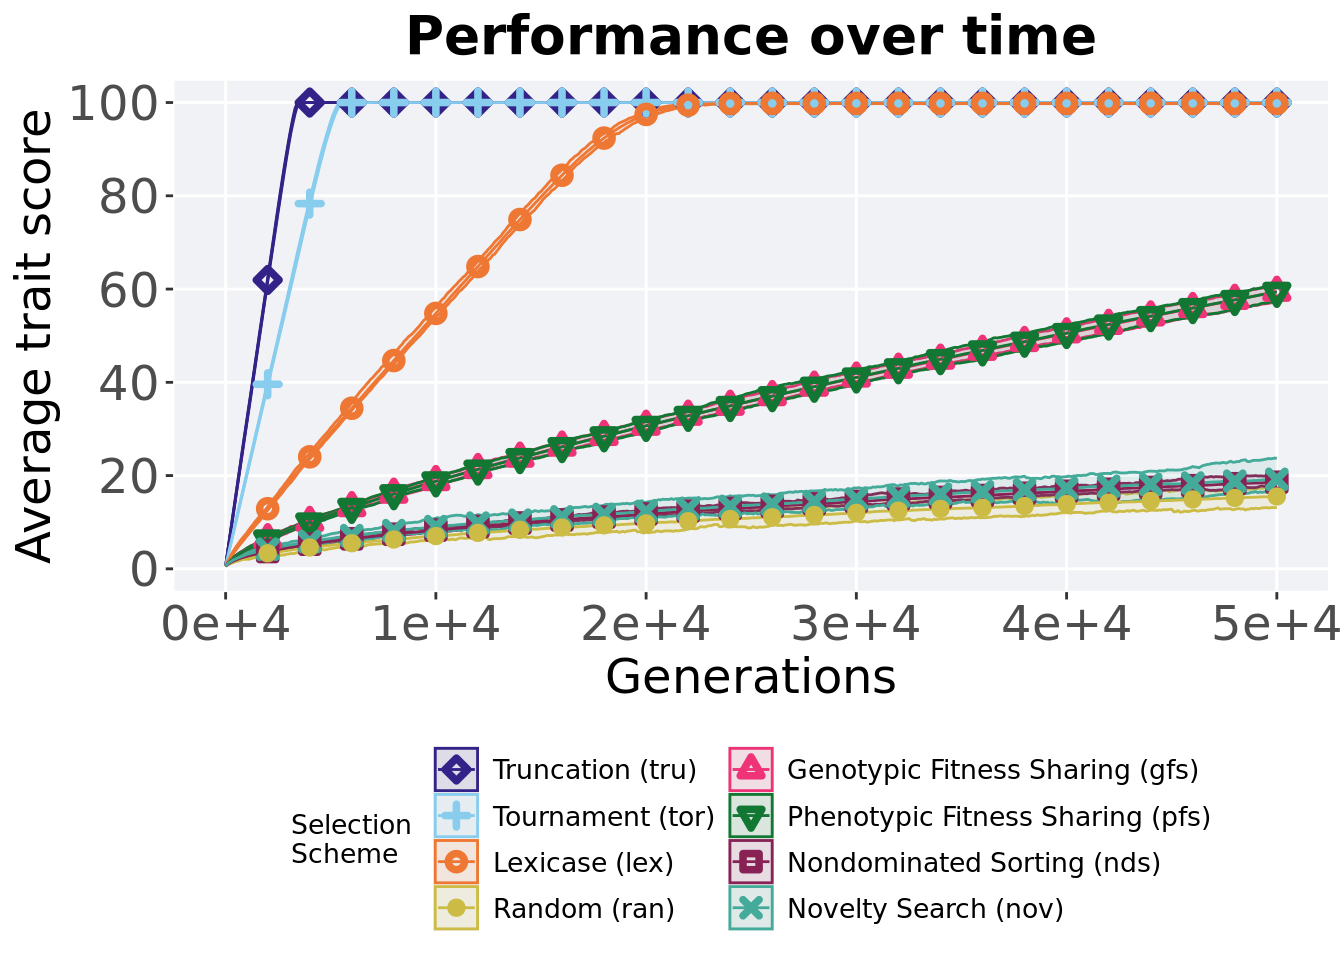
\includegraphics{mvc-diagnostics_files/figure-latex/exp-per-ot-1.pdf}

\hypertarget{best-performance-throughout}{%
\section{Best performance throughout}\label{best-performance-throughout}}

Best performance reached throughout 50,000 generations in a population.

\begin{Shaded}
\begin{Highlighting}[]
\NormalTok{plot =}\StringTok{ }\KeywordTok{filter}\NormalTok{(best_df, var }\OperatorTok{==}\StringTok{ 'pop_fit_max'}\NormalTok{) }\OperatorTok
\StringTok{  }\KeywordTok{ggplot}\NormalTok{(., }\KeywordTok{aes}\NormalTok{(}\DataTypeTok{x =}\NormalTok{ acro, }\DataTypeTok{y =}\NormalTok{ val }\OperatorTok{/}\StringTok{ }\NormalTok{DIMENSIONALITY, }\DataTypeTok{color =}\NormalTok{ acro, }\DataTypeTok{fill =}\NormalTok{ acro, }\DataTypeTok{shape =}\NormalTok{ acro)) }\OperatorTok{+}
\StringTok{  }\KeywordTok{geom_flat_violin}\NormalTok{(}\DataTypeTok{position =} \KeywordTok{position_nudge}\NormalTok{(}\DataTypeTok{x =} \FloatTok{.09}\NormalTok{, }\DataTypeTok{y =} \DecValTok{0}\NormalTok{), }\DataTypeTok{scale =} \StringTok{'width'}\NormalTok{, }\DataTypeTok{alpha =} \FloatTok{0.2}\NormalTok{, }\DataTypeTok{width =} \FloatTok{1.5}\NormalTok{) }\OperatorTok{+}
\StringTok{  }\KeywordTok{geom_boxplot}\NormalTok{(}\DataTypeTok{color =} \StringTok{'black'}\NormalTok{, }\DataTypeTok{width =} \FloatTok{.07}\NormalTok{, }\DataTypeTok{outlier.shape =} \OtherTok{NA}\NormalTok{, }\DataTypeTok{alpha =} \FloatTok{0.0}\NormalTok{, }\DataTypeTok{size =} \FloatTok{1.0}\NormalTok{, }\DataTypeTok{position =} \KeywordTok{position_nudge}\NormalTok{(}\DataTypeTok{x =} \FloatTok{.15}\NormalTok{, }\DataTypeTok{y =} \DecValTok{0}\NormalTok{)) }\OperatorTok{+}
\StringTok{  }\KeywordTok{geom_point}\NormalTok{(}\DataTypeTok{position =} \KeywordTok{position_jitter}\NormalTok{(}\DataTypeTok{width =} \FloatTok{.02}\NormalTok{), }\DataTypeTok{size =} \FloatTok{2.0}\NormalTok{, }\DataTypeTok{alpha =} \FloatTok{1.0}\NormalTok{) }\OperatorTok{+}
\StringTok{  }\KeywordTok{scale_y_continuous}\NormalTok{(}
    \DataTypeTok{name=}\StringTok{"Average trait score"}\NormalTok{,}
    \DataTypeTok{limits=}\KeywordTok{c}\NormalTok{(}\DecValTok{0}\NormalTok{, }\DecValTok{50}\NormalTok{),}
    \DataTypeTok{breaks=}\KeywordTok{seq}\NormalTok{(}\DecValTok{0}\NormalTok{,}\DecValTok{50}\NormalTok{, }\DecValTok{10}\NormalTok{),}
    \DataTypeTok{labels=}\KeywordTok{c}\NormalTok{(}\StringTok{"0"}\NormalTok{, }\StringTok{"10"}\NormalTok{, }\StringTok{"20"}\NormalTok{, }\StringTok{"30"}\NormalTok{, }\StringTok{"40"}\NormalTok{, }\StringTok{"50"}\NormalTok{)}
\NormalTok{  ) }\OperatorTok{+}
\StringTok{  }\KeywordTok{scale_x_discrete}\NormalTok{(}
    \DataTypeTok{name=}\StringTok{"Scheme"}
\NormalTok{  )}\OperatorTok{+}
\StringTok{  }\KeywordTok{scale_shape_manual}\NormalTok{(}\DataTypeTok{values=}\NormalTok{SHAPE)}\OperatorTok{+}
\StringTok{  }\KeywordTok{scale_colour_manual}\NormalTok{(}\DataTypeTok{values =}\NormalTok{ cb_palette, ) }\OperatorTok{+}
\StringTok{  }\KeywordTok{scale_fill_manual}\NormalTok{(}\DataTypeTok{values =}\NormalTok{ cb_palette) }\OperatorTok{+}
\StringTok{  }\KeywordTok{ggtitle}\NormalTok{(}\StringTok{'Best performance throughout'}\NormalTok{)}\OperatorTok{+}
\StringTok{  }\NormalTok{p_theme }\OperatorTok{+}\StringTok{ }\KeywordTok{theme}\NormalTok{(}\DataTypeTok{legend.title=}\KeywordTok{element_blank}\NormalTok{())}

\KeywordTok{plot_grid}\NormalTok{(}
\NormalTok{  plot }\OperatorTok{+}
\StringTok{    }\KeywordTok{theme}\NormalTok{(}\DataTypeTok{legend.position=}\StringTok{"none"}\NormalTok{),}
\NormalTok{  legend,}
  \DataTypeTok{nrow=}\DecValTok{2}\NormalTok{,}
  \DataTypeTok{rel_heights =} \KeywordTok{c}\NormalTok{(}\DecValTok{3}\NormalTok{,}\DecValTok{1}\NormalTok{)}
\NormalTok{)}
\end{Highlighting}
\end{Shaded}

\begin{verbatim}
## Warning: Using the `size` aesthetic with geom_polygon was deprecated in ggplot2 3.4.0.
## i Please use the `linewidth` aesthetic instead.
## This warning is displayed once every 8 hours.
## Call `lifecycle::last_lifecycle_warnings()` to see where this warning was
## generated.
\end{verbatim}

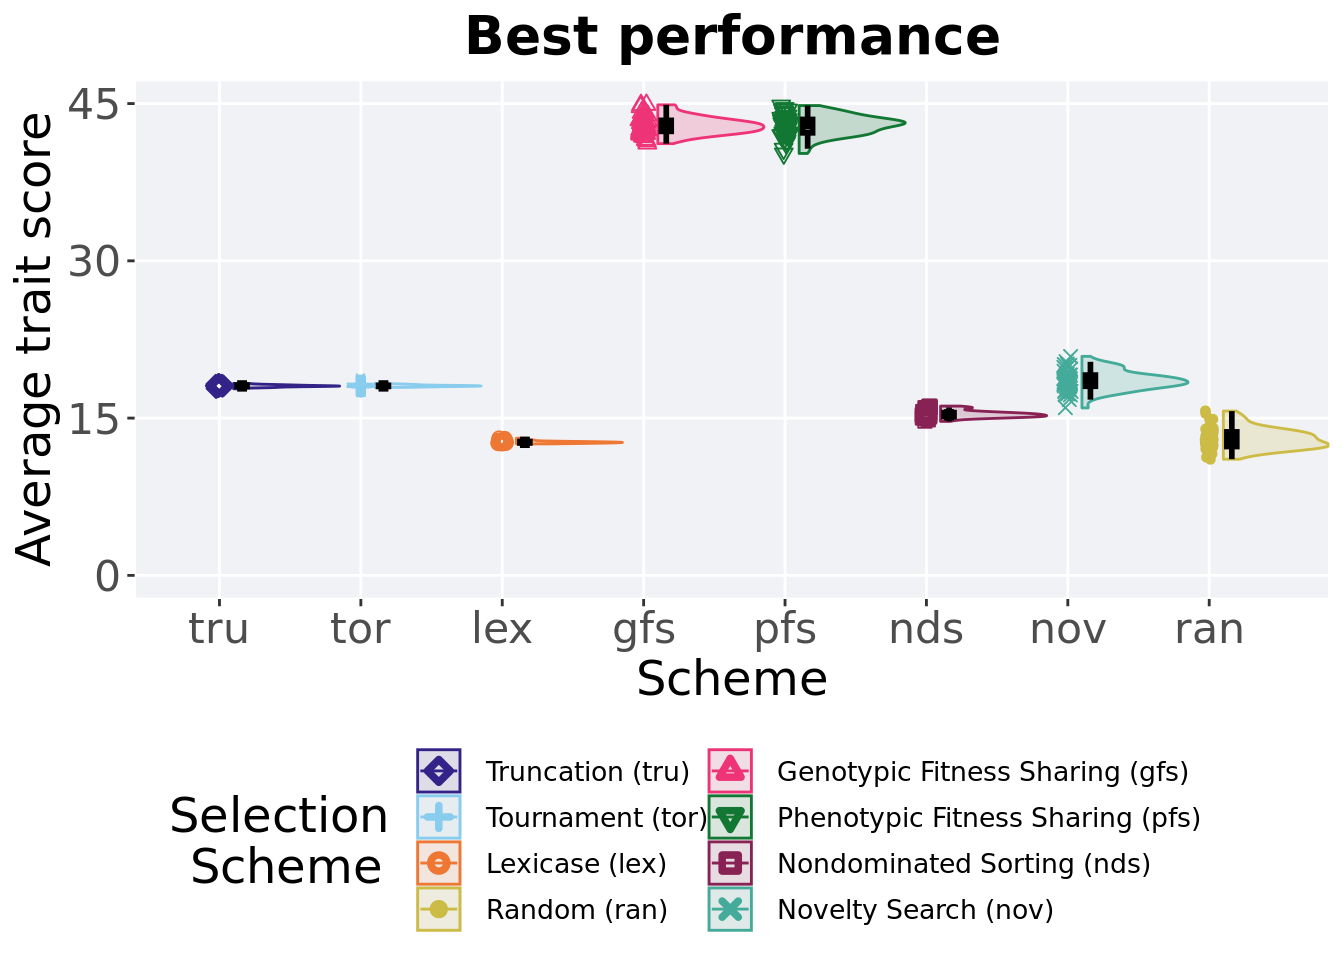
\includegraphics{mvc-diagnostics_files/figure-latex/exp-per-bst-1.pdf}

\hypertarget{stats}{%
\subsection{Stats}\label{stats}}

Summary statistics for the best performance.

\begin{Shaded}
\begin{Highlighting}[]
\NormalTok{performance =}\StringTok{ }\KeywordTok{filter}\NormalTok{(best_df, var }\OperatorTok{==}\StringTok{ 'pop_fit_max'}\NormalTok{)}
\NormalTok{performance}\OperatorTok{$}\NormalTok{acro =}\StringTok{ }\KeywordTok{factor}\NormalTok{(performance}\OperatorTok{$}\NormalTok{acro, }\DataTypeTok{levels =} \KeywordTok{c}\NormalTok{(}\StringTok{'gfs'}\NormalTok{,}\StringTok{'pfs'}\NormalTok{,}\StringTok{'tru'}\NormalTok{,}\StringTok{'tor'}\NormalTok{,}\StringTok{'nov'}\NormalTok{,}\StringTok{'nds'}\NormalTok{,}\StringTok{'ran'}\NormalTok{,}\StringTok{'lex'}\NormalTok{))}
\NormalTok{performance }\OperatorTok
\StringTok{  }\KeywordTok{group_by}\NormalTok{(acro) }\OperatorTok
\StringTok{  }\NormalTok{dplyr}\OperatorTok{::}\KeywordTok{summarise}\NormalTok{(}
    \DataTypeTok{count =} \KeywordTok{n}\NormalTok{(),}
    \DataTypeTok{na_cnt =} \KeywordTok{sum}\NormalTok{(}\KeywordTok{is.na}\NormalTok{(val)),}
    \DataTypeTok{min =} \KeywordTok{min}\NormalTok{(val }\OperatorTok{/}\StringTok{ }\NormalTok{DIMENSIONALITY, }\DataTypeTok{na.rm =} \OtherTok{TRUE}\NormalTok{),}
    \DataTypeTok{median =} \KeywordTok{median}\NormalTok{(val }\OperatorTok{/}\StringTok{ }\NormalTok{DIMENSIONALITY, }\DataTypeTok{na.rm =} \OtherTok{TRUE}\NormalTok{),}
    \DataTypeTok{mean =} \KeywordTok{mean}\NormalTok{(val }\OperatorTok{/}\StringTok{ }\NormalTok{DIMENSIONALITY, }\DataTypeTok{na.rm =} \OtherTok{TRUE}\NormalTok{),}
    \DataTypeTok{max =} \KeywordTok{max}\NormalTok{(val }\OperatorTok{/}\StringTok{ }\NormalTok{DIMENSIONALITY, }\DataTypeTok{na.rm =} \OtherTok{TRUE}\NormalTok{),}
    \DataTypeTok{IQR =} \KeywordTok{IQR}\NormalTok{(val }\OperatorTok{/}\StringTok{ }\NormalTok{DIMENSIONALITY, }\DataTypeTok{na.rm =} \OtherTok{TRUE}\NormalTok{)}
\NormalTok{  )}
\end{Highlighting}
\end{Shaded}

\begin{verbatim}
## # A tibble: 8 x 8
##   acro  count na_cnt   min median  mean   max   IQR
##   <fct> <int>  <int> <dbl>  <dbl> <dbl> <dbl> <dbl>
## 1 gfs      50      0  41.0   43.2  43.2  45.2 0.923
## 2 pfs      50      0  41.2   43.0  42.9  45.6 1.17 
## 3 tru      50      0  17.8   18.1  18.0  18.3 0.140
## 4 tor      50      0  17.9   18.1  18.1  18.3 0.150
## 5 nov      50      0  16.4   18.8  18.7  20.4 1.51 
## 6 nds      50      0  14.8   15.3  15.4  16.6 0.418
## 7 ran      50      0  11.0   13.2  13.1  15.2 0.900
## 8 lex      50      0  12.5   12.7  12.7  13.0 0.154
\end{verbatim}

Kruskal--Wallis test illustrates evidence of statistical differences.

\begin{Shaded}
\begin{Highlighting}[]
\KeywordTok{kruskal.test}\NormalTok{(val }\OperatorTok{~}\StringTok{ }\NormalTok{acro, }\DataTypeTok{data =}\NormalTok{ performance)}
\end{Highlighting}
\end{Shaded}

\begin{verbatim}
## 
##  Kruskal-Wallis rank sum test
## 
## data:  val by acro
## Kruskal-Wallis chi-squared = 367.97, df = 7, p-value < 2.2e-16
\end{verbatim}

Results for post-hoc Wilcoxon rank-sum test with a Bonferroni correction.

\begin{Shaded}
\begin{Highlighting}[]
\KeywordTok{pairwise.wilcox.test}\NormalTok{(}\DataTypeTok{x =}\NormalTok{ performance}\OperatorTok{$}\NormalTok{val, }\DataTypeTok{g =}\NormalTok{ performance}\OperatorTok{$}\NormalTok{acro, }\DataTypeTok{p.adjust.method =} \StringTok{"bonferroni"}\NormalTok{,}
                     \DataTypeTok{paired =} \OtherTok{FALSE}\NormalTok{, }\DataTypeTok{conf.int =} \OtherTok{FALSE}\NormalTok{, }\DataTypeTok{alternative =} \StringTok{'l'}\NormalTok{)}
\end{Highlighting}
\end{Shaded}

\begin{verbatim}
## 
##  Pairwise comparisons using Wilcoxon rank sum test with continuity correction 
## 
## data:  performance$val and performance$acro 
## 
##     gfs     pfs     tru     tor     nov     nds     ran   
## pfs 0.4845  -       -       -       -       -       -     
## tru < 2e-16 < 2e-16 -       -       -       -       -     
## tor < 2e-16 < 2e-16 1.0000  -       -       -       -     
## nov < 2e-16 < 2e-16 1.0000  1.0000  -       -       -     
## nds < 2e-16 < 2e-16 < 2e-16 < 2e-16 < 2e-16 -       -     
## ran < 2e-16 < 2e-16 < 2e-16 < 2e-16 < 2e-16 2.9e-16 -     
## lex < 2e-16 < 2e-16 < 2e-16 < 2e-16 < 2e-16 < 2e-16 0.0035
## 
## P value adjustment method: bonferroni
\end{verbatim}

\hypertarget{performance-interval-comparison}{%
\section{Performance interval comparison}\label{performance-interval-comparison}}

Here we compare the best performance found in the population at generation 40,000 \& 50,000 for all selection schemes.

\begin{Shaded}
\begin{Highlighting}[]
\NormalTok{interval_df =}\StringTok{ }\KeywordTok{filter}\NormalTok{(}\KeywordTok{filter}\NormalTok{(over_time_df, (gen }\OperatorTok{==}\StringTok{ }\DecValTok{50000} \OperatorTok{|}\StringTok{ }\NormalTok{gen }\OperatorTok{==}\StringTok{ }\DecValTok{40000}\NormalTok{)))}
\NormalTok{interval_df}\OperatorTok{$}\NormalTok{Generation <-}\StringTok{ }\KeywordTok{factor}\NormalTok{(interval_df}\OperatorTok{$}\NormalTok{gen, }\DataTypeTok{levels =} \KeywordTok{c}\NormalTok{(}\DecValTok{40000}\NormalTok{,}\DecValTok{50000}\NormalTok{))}
\NormalTok{interval_df}\OperatorTok{$}\NormalTok{acro <-}\StringTok{ }\KeywordTok{factor}\NormalTok{(interval_df}\OperatorTok{$}\NormalTok{acro, }\DataTypeTok{levels =}\NormalTok{ ACRO)}

\KeywordTok{ggplot}\NormalTok{(interval_df, }\KeywordTok{aes}\NormalTok{(}\DataTypeTok{x=}\NormalTok{acro, }\DataTypeTok{y=}\NormalTok{pop_fit_max}\OperatorTok{/}\NormalTok{DIMENSIONALITY,}\DataTypeTok{fill=}\NormalTok{Generation,}\DataTypeTok{color=}\NormalTok{Generation,}\DataTypeTok{shape=}\NormalTok{Generation)) }\OperatorTok{+}
\StringTok{  }\KeywordTok{geom_boxplot}\NormalTok{(}\DataTypeTok{width =} \FloatTok{.3}\NormalTok{, }\DataTypeTok{outlier.shape =} \OtherTok{NA}\NormalTok{, }\DataTypeTok{alpha =} \FloatTok{0.0}\NormalTok{) }\OperatorTok{+}
\StringTok{    }\KeywordTok{geom_point}\NormalTok{(}\DataTypeTok{size =} \FloatTok{1.0}\NormalTok{, }\DataTypeTok{alpha =} \FloatTok{1.0}\NormalTok{, }\DataTypeTok{position=}\KeywordTok{position_dodge}\NormalTok{(}\DataTypeTok{width=}\FloatTok{1.0}\NormalTok{)) }\OperatorTok{+}
\StringTok{    }\KeywordTok{scale_y_continuous}\NormalTok{(}
      \DataTypeTok{name=}\StringTok{"Average trait score"}\NormalTok{,}
      \DataTypeTok{limits=}\KeywordTok{c}\NormalTok{(}\DecValTok{0}\NormalTok{, }\DecValTok{50}\NormalTok{),}
      \DataTypeTok{breaks=}\KeywordTok{seq}\NormalTok{(}\DecValTok{0}\NormalTok{,}\DecValTok{50}\NormalTok{, }\DecValTok{10}\NormalTok{),}
      \DataTypeTok{labels=}\KeywordTok{c}\NormalTok{(}\StringTok{"0"}\NormalTok{,}\StringTok{"10"}\NormalTok{, }\StringTok{"20"}\NormalTok{, }\StringTok{"30"}\NormalTok{, }\StringTok{"40"}\NormalTok{, }\StringTok{"50"}\NormalTok{)}
\NormalTok{    ) }\OperatorTok{+}
\StringTok{    }\KeywordTok{scale_x_discrete}\NormalTok{(}
      \DataTypeTok{name=}\StringTok{"Scheme"}
\NormalTok{    ) }\OperatorTok{+}
\StringTok{  }\KeywordTok{scale_shape_manual}\NormalTok{(}\DataTypeTok{values=}\NormalTok{SHAPE)}\OperatorTok{+}
\StringTok{  }\KeywordTok{scale_colour_manual}\NormalTok{(}\DataTypeTok{values =}\NormalTok{ mvc_col, ) }\OperatorTok{+}
\StringTok{  }\KeywordTok{scale_fill_manual}\NormalTok{(}\DataTypeTok{values =}\NormalTok{ mvc_col) }\OperatorTok{+}
\StringTok{  }\KeywordTok{ggtitle}\NormalTok{(}\StringTok{'Performance comparisons'}\NormalTok{)}\OperatorTok{+}
\StringTok{  }\NormalTok{p_theme}
\end{Highlighting}
\end{Shaded}

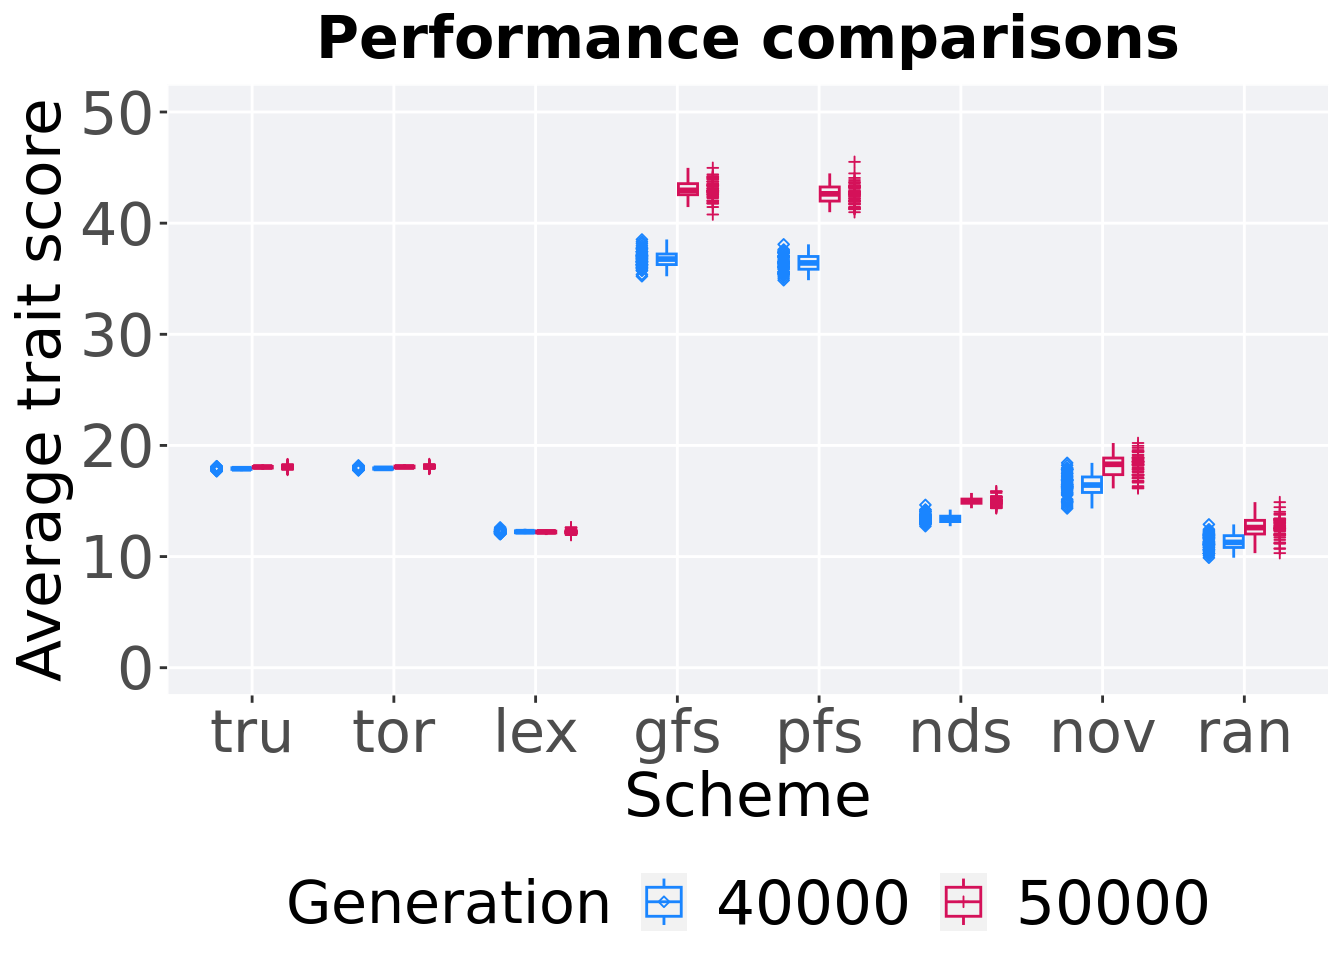
\includegraphics{mvc-diagnostics_files/figure-latex/exp-per-cmp-1.pdf}

\hypertarget{stats-by-interval-comparisons}{%
\subsection{Stats by interval comparisons}\label{stats-by-interval-comparisons}}

Here we present statistical analysis between the performances found at different generation intervals.

\hypertarget{truncation}{%
\subsubsection{Truncation}\label{truncation}}

Plot for comparing performances at interval 40,000 \& 50,000.

\begin{Shaded}
\begin{Highlighting}[]
\KeywordTok{filter}\NormalTok{(interval_df, acro }\OperatorTok{==}\StringTok{ 'tru'}\NormalTok{) }\OperatorTok
\KeywordTok{ggplot}\NormalTok{(., }\KeywordTok{aes}\NormalTok{(}\DataTypeTok{x=}\NormalTok{Generation, }\DataTypeTok{y=}\NormalTok{pop_fit_max}\OperatorTok{/}\NormalTok{DIMENSIONALITY,}\DataTypeTok{fill=}\NormalTok{Generation,}\DataTypeTok{color=}\NormalTok{Generation,}\DataTypeTok{shape=}\NormalTok{Generation)) }\OperatorTok{+}
\StringTok{  }\KeywordTok{geom_flat_violin}\NormalTok{(}\DataTypeTok{position =} \KeywordTok{position_nudge}\NormalTok{(}\DataTypeTok{x =} \FloatTok{.09}\NormalTok{, }\DataTypeTok{y =} \DecValTok{0}\NormalTok{), }\DataTypeTok{scale =} \StringTok{'width'}\NormalTok{, }\DataTypeTok{alpha =} \FloatTok{0.2}\NormalTok{, }\DataTypeTok{width =} \FloatTok{1.5}\NormalTok{) }\OperatorTok{+}
\StringTok{  }\KeywordTok{geom_boxplot}\NormalTok{(}\DataTypeTok{color =} \StringTok{'black'}\NormalTok{, }\DataTypeTok{width =} \FloatTok{.07}\NormalTok{, }\DataTypeTok{outlier.shape =} \OtherTok{NA}\NormalTok{, }\DataTypeTok{alpha =} \FloatTok{0.0}\NormalTok{, }\DataTypeTok{size =} \FloatTok{1.0}\NormalTok{, }\DataTypeTok{position =} \KeywordTok{position_nudge}\NormalTok{(}\DataTypeTok{x =} \FloatTok{.15}\NormalTok{, }\DataTypeTok{y =} \DecValTok{0}\NormalTok{)) }\OperatorTok{+}
\StringTok{  }\KeywordTok{geom_point}\NormalTok{(}\DataTypeTok{position =} \KeywordTok{position_jitter}\NormalTok{(}\DataTypeTok{width =} \FloatTok{.02}\NormalTok{), }\DataTypeTok{size =} \FloatTok{2.0}\NormalTok{, }\DataTypeTok{alpha =} \FloatTok{1.0}\NormalTok{) }\OperatorTok{+}
\StringTok{    }\KeywordTok{scale_y_continuous}\NormalTok{(}
      \DataTypeTok{name=}\StringTok{"Average trait score"}\NormalTok{,}
\NormalTok{    ) }\OperatorTok{+}
\StringTok{    }\KeywordTok{scale_x_discrete}\NormalTok{(}
      \DataTypeTok{name=}\StringTok{"Generation"}
\NormalTok{    ) }\OperatorTok{+}
\StringTok{  }\KeywordTok{scale_shape_manual}\NormalTok{(}\DataTypeTok{values=}\KeywordTok{c}\NormalTok{(}\DecValTok{16}\NormalTok{,}\DecValTok{16}\NormalTok{))}\OperatorTok{+}
\StringTok{  }\KeywordTok{scale_colour_manual}\NormalTok{(}\DataTypeTok{values =}\NormalTok{ mvc_col, ) }\OperatorTok{+}
\StringTok{  }\KeywordTok{scale_fill_manual}\NormalTok{(}\DataTypeTok{values =}\NormalTok{ mvc_col) }\OperatorTok{+}
\StringTok{  }\KeywordTok{ggtitle}\NormalTok{(}\StringTok{'Performance comparisons'}\NormalTok{)}\OperatorTok{+}
\StringTok{  }\NormalTok{p_theme }\OperatorTok{+}\StringTok{ }\KeywordTok{theme}\NormalTok{(}\DataTypeTok{legend.position=}\StringTok{"none"}\NormalTok{)}
\end{Highlighting}
\end{Shaded}

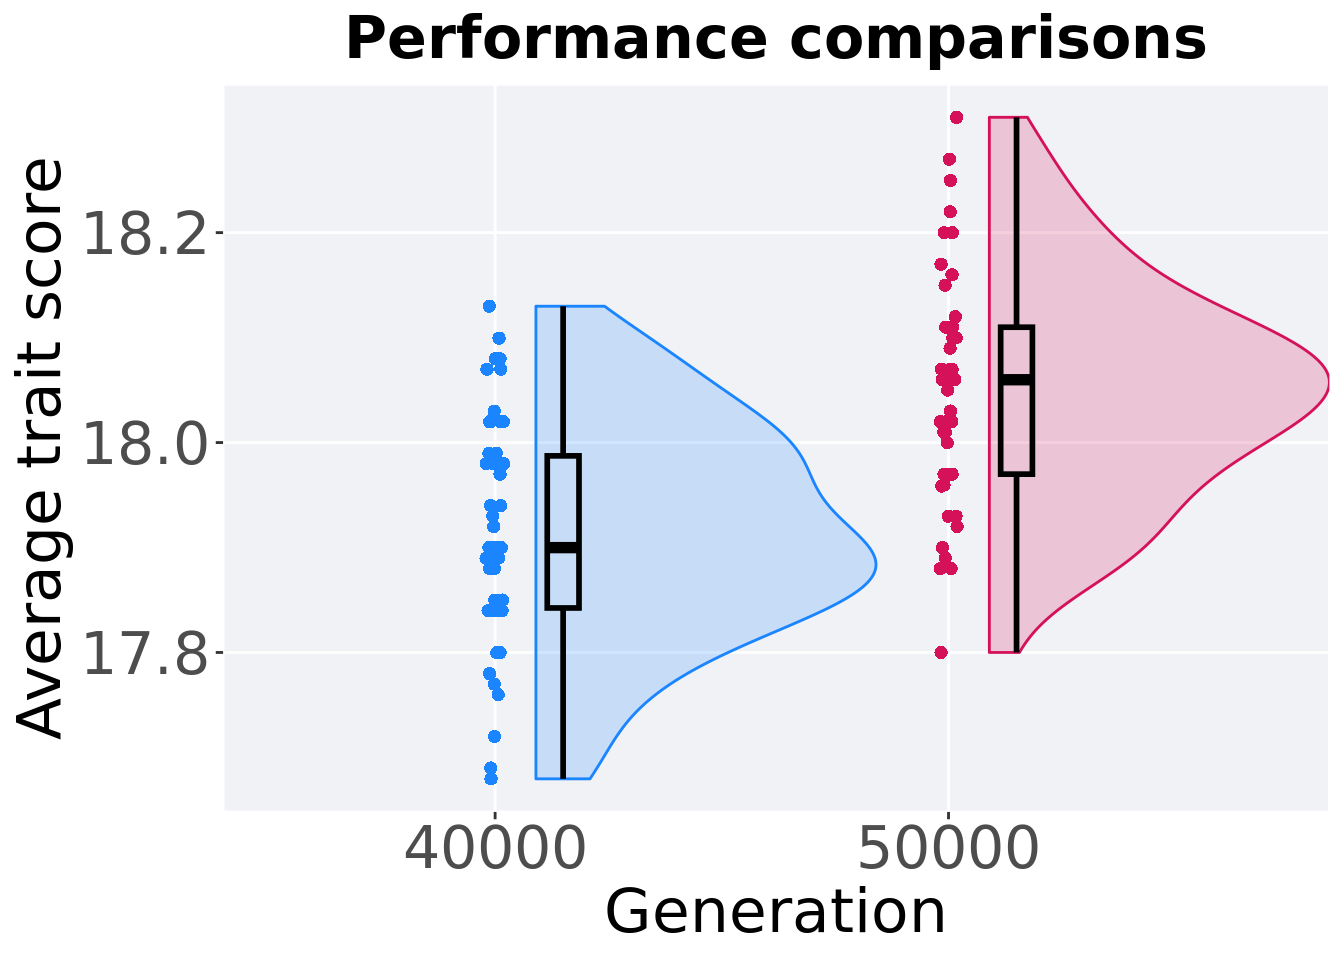
\includegraphics{mvc-diagnostics_files/figure-latex/exp-per-cmp-plt-tru-1.pdf}

Summary statistics for the best performance.

\begin{Shaded}
\begin{Highlighting}[]
\KeywordTok{filter}\NormalTok{(interval_df, acro }\OperatorTok{==}\StringTok{ 'tru'}\NormalTok{) }\OperatorTok
\StringTok{  }\KeywordTok{group_by}\NormalTok{(Generation) }\OperatorTok
\StringTok{  }\NormalTok{dplyr}\OperatorTok{::}\KeywordTok{summarise}\NormalTok{(}
    \DataTypeTok{count =} \KeywordTok{n}\NormalTok{(),}
    \DataTypeTok{na_cnt =} \KeywordTok{sum}\NormalTok{(}\KeywordTok{is.na}\NormalTok{(pop_fit_max)),}
    \DataTypeTok{min =} \KeywordTok{min}\NormalTok{(pop_fit_max }\OperatorTok{/}\StringTok{ }\NormalTok{DIMENSIONALITY, }\DataTypeTok{na.rm =} \OtherTok{TRUE}\NormalTok{),}
    \DataTypeTok{median =} \KeywordTok{median}\NormalTok{(pop_fit_max }\OperatorTok{/}\StringTok{ }\NormalTok{DIMENSIONALITY, }\DataTypeTok{na.rm =} \OtherTok{TRUE}\NormalTok{),}
    \DataTypeTok{mean =} \KeywordTok{mean}\NormalTok{(pop_fit_max }\OperatorTok{/}\StringTok{ }\NormalTok{DIMENSIONALITY, }\DataTypeTok{na.rm =} \OtherTok{TRUE}\NormalTok{),}
    \DataTypeTok{max =} \KeywordTok{max}\NormalTok{(pop_fit_max }\OperatorTok{/}\StringTok{ }\NormalTok{DIMENSIONALITY, }\DataTypeTok{na.rm =} \OtherTok{TRUE}\NormalTok{),}
    \DataTypeTok{IQR =} \KeywordTok{IQR}\NormalTok{(pop_fit_max }\OperatorTok{/}\StringTok{ }\NormalTok{DIMENSIONALITY, }\DataTypeTok{na.rm =} \OtherTok{TRUE}\NormalTok{)}
\NormalTok{  )}
\end{Highlighting}
\end{Shaded}

\begin{verbatim}
## # A tibble: 2 x 8
##   Generation count na_cnt   min median  mean   max   IQR
##   <fct>      <int>  <int> <dbl>  <dbl> <dbl> <dbl> <dbl>
## 1 40000         50      0  17.7   17.9  17.9  18.1 0.145
## 2 50000         50      0  17.8   18.1  18.0  18.3 0.140
\end{verbatim}

Results for post-hoc Wilcoxon rank-sum test.

\begin{Shaded}
\begin{Highlighting}[]
\KeywordTok{wilcox.test}\NormalTok{(}\DataTypeTok{x =} \KeywordTok{filter}\NormalTok{(interval_df, acro }\OperatorTok{==}\StringTok{ 'tru'} \OperatorTok{&}\StringTok{ }\NormalTok{Generation }\OperatorTok{==}\StringTok{ }\DecValTok{50000}\NormalTok{)}\OperatorTok{$}\NormalTok{pop_fit_max,}
            \DataTypeTok{y =} \KeywordTok{filter}\NormalTok{(interval_df, acro }\OperatorTok{==}\StringTok{ 'tru'} \OperatorTok{&}\StringTok{ }\NormalTok{Generation }\OperatorTok{==}\StringTok{ }\DecValTok{40000}\NormalTok{)}\OperatorTok{$}\NormalTok{pop_fit_max,}
            \DataTypeTok{alternative =} \StringTok{'g'}\NormalTok{)}
\end{Highlighting}
\end{Shaded}

\begin{verbatim}
## 
##  Wilcoxon rank sum test with continuity correction
## 
## data:  filter(interval_df, acro == "tru" & Generation == 50000)$pop_fit_max and filter(interval_df, acro == "tru" & Generation == 40000)$pop_fit_max
## W = 2013.5, p-value = 7.103e-08
## alternative hypothesis: true location shift is greater than 0
\end{verbatim}

\hypertarget{tournament}{%
\subsubsection{Tournament}\label{tournament}}

Plot for comparing performances at interval 40,000 \& 50,000.

\begin{Shaded}
\begin{Highlighting}[]
\KeywordTok{filter}\NormalTok{(interval_df, acro }\OperatorTok{==}\StringTok{ 'tor'}\NormalTok{) }\OperatorTok
\KeywordTok{ggplot}\NormalTok{(., }\KeywordTok{aes}\NormalTok{(}\DataTypeTok{x=}\NormalTok{Generation, }\DataTypeTok{y=}\NormalTok{pop_fit_max}\OperatorTok{/}\NormalTok{DIMENSIONALITY,}\DataTypeTok{fill=}\NormalTok{Generation,}\DataTypeTok{color=}\NormalTok{Generation,}\DataTypeTok{shape=}\NormalTok{Generation)) }\OperatorTok{+}
\StringTok{  }\KeywordTok{geom_flat_violin}\NormalTok{(}\DataTypeTok{position =} \KeywordTok{position_nudge}\NormalTok{(}\DataTypeTok{x =} \FloatTok{.09}\NormalTok{, }\DataTypeTok{y =} \DecValTok{0}\NormalTok{), }\DataTypeTok{scale =} \StringTok{'width'}\NormalTok{, }\DataTypeTok{alpha =} \FloatTok{0.2}\NormalTok{, }\DataTypeTok{width =} \FloatTok{1.5}\NormalTok{) }\OperatorTok{+}
\StringTok{  }\KeywordTok{geom_boxplot}\NormalTok{(}\DataTypeTok{color =} \StringTok{'black'}\NormalTok{, }\DataTypeTok{width =} \FloatTok{.07}\NormalTok{, }\DataTypeTok{outlier.shape =} \OtherTok{NA}\NormalTok{, }\DataTypeTok{alpha =} \FloatTok{0.0}\NormalTok{, }\DataTypeTok{size =} \FloatTok{1.0}\NormalTok{, }\DataTypeTok{position =} \KeywordTok{position_nudge}\NormalTok{(}\DataTypeTok{x =} \FloatTok{.15}\NormalTok{, }\DataTypeTok{y =} \DecValTok{0}\NormalTok{)) }\OperatorTok{+}
\StringTok{  }\KeywordTok{geom_point}\NormalTok{(}\DataTypeTok{position =} \KeywordTok{position_jitter}\NormalTok{(}\DataTypeTok{width =} \FloatTok{.02}\NormalTok{), }\DataTypeTok{size =} \FloatTok{2.0}\NormalTok{, }\DataTypeTok{alpha =} \FloatTok{1.0}\NormalTok{) }\OperatorTok{+}
\StringTok{    }\KeywordTok{scale_y_continuous}\NormalTok{(}
      \DataTypeTok{name=}\StringTok{"Average trait score"}\NormalTok{,}
\NormalTok{    ) }\OperatorTok{+}
\StringTok{    }\KeywordTok{scale_x_discrete}\NormalTok{(}
      \DataTypeTok{name=}\StringTok{"Generation"}
\NormalTok{    ) }\OperatorTok{+}
\StringTok{  }\KeywordTok{scale_shape_manual}\NormalTok{(}\DataTypeTok{values=}\KeywordTok{c}\NormalTok{(}\DecValTok{16}\NormalTok{,}\DecValTok{16}\NormalTok{))}\OperatorTok{+}
\StringTok{  }\KeywordTok{scale_colour_manual}\NormalTok{(}\DataTypeTok{values =}\NormalTok{ mvc_col, ) }\OperatorTok{+}
\StringTok{  }\KeywordTok{scale_fill_manual}\NormalTok{(}\DataTypeTok{values =}\NormalTok{ mvc_col) }\OperatorTok{+}
\StringTok{  }\KeywordTok{ggtitle}\NormalTok{(}\StringTok{'Performance comparisons'}\NormalTok{)}\OperatorTok{+}
\StringTok{  }\NormalTok{p_theme }\OperatorTok{+}\StringTok{ }\KeywordTok{theme}\NormalTok{(}\DataTypeTok{legend.position=}\StringTok{"none"}\NormalTok{)}
\end{Highlighting}
\end{Shaded}

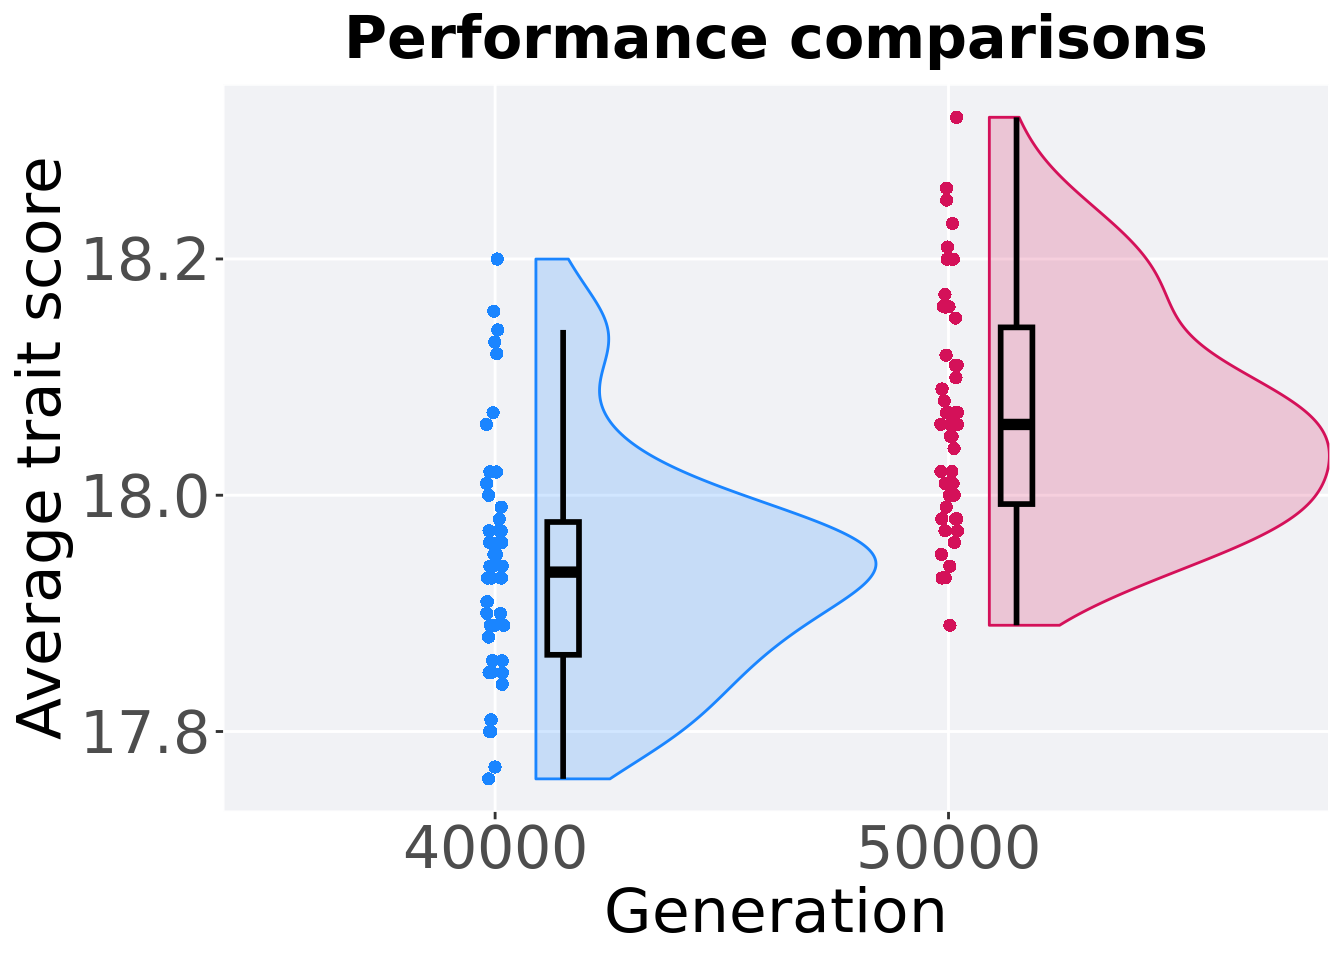
\includegraphics{mvc-diagnostics_files/figure-latex/exp-per-cmp-plt-tor-1.pdf}

Summary statistics for the best performance.

\begin{Shaded}
\begin{Highlighting}[]
\KeywordTok{filter}\NormalTok{(interval_df, acro }\OperatorTok{==}\StringTok{ 'tor'}\NormalTok{) }\OperatorTok
\StringTok{  }\KeywordTok{group_by}\NormalTok{(Generation) }\OperatorTok
\StringTok{  }\NormalTok{dplyr}\OperatorTok{::}\KeywordTok{summarise}\NormalTok{(}
    \DataTypeTok{count =} \KeywordTok{n}\NormalTok{(),}
    \DataTypeTok{na_cnt =} \KeywordTok{sum}\NormalTok{(}\KeywordTok{is.na}\NormalTok{(pop_fit_max)),}
    \DataTypeTok{min =} \KeywordTok{min}\NormalTok{(pop_fit_max }\OperatorTok{/}\StringTok{ }\NormalTok{DIMENSIONALITY, }\DataTypeTok{na.rm =} \OtherTok{TRUE}\NormalTok{),}
    \DataTypeTok{median =} \KeywordTok{median}\NormalTok{(pop_fit_max }\OperatorTok{/}\StringTok{ }\NormalTok{DIMENSIONALITY, }\DataTypeTok{na.rm =} \OtherTok{TRUE}\NormalTok{),}
    \DataTypeTok{mean =} \KeywordTok{mean}\NormalTok{(pop_fit_max }\OperatorTok{/}\StringTok{ }\NormalTok{DIMENSIONALITY, }\DataTypeTok{na.rm =} \OtherTok{TRUE}\NormalTok{),}
    \DataTypeTok{max =} \KeywordTok{max}\NormalTok{(pop_fit_max }\OperatorTok{/}\StringTok{ }\NormalTok{DIMENSIONALITY, }\DataTypeTok{na.rm =} \OtherTok{TRUE}\NormalTok{),}
    \DataTypeTok{IQR =} \KeywordTok{IQR}\NormalTok{(pop_fit_max }\OperatorTok{/}\StringTok{ }\NormalTok{DIMENSIONALITY, }\DataTypeTok{na.rm =} \OtherTok{TRUE}\NormalTok{)}
\NormalTok{  )}
\end{Highlighting}
\end{Shaded}

\begin{verbatim}
## # A tibble: 2 x 8
##   Generation count na_cnt   min median  mean   max   IQR
##   <fct>      <int>  <int> <dbl>  <dbl> <dbl> <dbl> <dbl>
## 1 40000         50      0  17.8   17.9  17.9  18.2 0.112
## 2 50000         50      0  17.9   18.1  18.1  18.3 0.150
\end{verbatim}

Results for post-hoc Wilcoxon rank-sum test.

\begin{Shaded}
\begin{Highlighting}[]
\KeywordTok{wilcox.test}\NormalTok{(}\DataTypeTok{x =} \KeywordTok{filter}\NormalTok{(interval_df, acro }\OperatorTok{==}\StringTok{ 'tor'} \OperatorTok{&}\StringTok{ }\NormalTok{Generation }\OperatorTok{==}\StringTok{ }\DecValTok{50000}\NormalTok{)}\OperatorTok{$}\NormalTok{pop_fit_max,}
            \DataTypeTok{y =} \KeywordTok{filter}\NormalTok{(interval_df, acro }\OperatorTok{==}\StringTok{ 'tor'} \OperatorTok{&}\StringTok{ }\NormalTok{Generation }\OperatorTok{==}\StringTok{ }\DecValTok{40000}\NormalTok{)}\OperatorTok{$}\NormalTok{pop_fit_max,}
            \DataTypeTok{alternative =} \StringTok{'g'}\NormalTok{)}
\end{Highlighting}
\end{Shaded}

\begin{verbatim}
## 
##  Wilcoxon rank sum test with continuity correction
## 
## data:  filter(interval_df, acro == "tor" & Generation == 50000)$pop_fit_max and filter(interval_df, acro == "tor" & Generation == 40000)$pop_fit_max
## W = 2095.5, p-value = 2.818e-09
## alternative hypothesis: true location shift is greater than 0
\end{verbatim}

\hypertarget{lexicase}{%
\subsubsection{Lexicase}\label{lexicase}}

Plot for comparing performances at interval 40,000 \& 50,000.

\begin{Shaded}
\begin{Highlighting}[]
\KeywordTok{filter}\NormalTok{(interval_df, acro }\OperatorTok{==}\StringTok{ 'lex'}\NormalTok{) }\OperatorTok
\KeywordTok{ggplot}\NormalTok{(., }\KeywordTok{aes}\NormalTok{(}\DataTypeTok{x=}\NormalTok{Generation, }\DataTypeTok{y=}\NormalTok{pop_fit_max}\OperatorTok{/}\NormalTok{DIMENSIONALITY,}\DataTypeTok{fill=}\NormalTok{Generation,}\DataTypeTok{color=}\NormalTok{Generation,}\DataTypeTok{shape=}\NormalTok{Generation)) }\OperatorTok{+}
\StringTok{  }\KeywordTok{geom_flat_violin}\NormalTok{(}\DataTypeTok{position =} \KeywordTok{position_nudge}\NormalTok{(}\DataTypeTok{x =} \FloatTok{.09}\NormalTok{, }\DataTypeTok{y =} \DecValTok{0}\NormalTok{), }\DataTypeTok{scale =} \StringTok{'width'}\NormalTok{, }\DataTypeTok{alpha =} \FloatTok{0.2}\NormalTok{, }\DataTypeTok{width =} \FloatTok{1.5}\NormalTok{) }\OperatorTok{+}
\StringTok{  }\KeywordTok{geom_boxplot}\NormalTok{(}\DataTypeTok{color =} \StringTok{'black'}\NormalTok{, }\DataTypeTok{width =} \FloatTok{.07}\NormalTok{, }\DataTypeTok{outlier.shape =} \OtherTok{NA}\NormalTok{, }\DataTypeTok{alpha =} \FloatTok{0.0}\NormalTok{, }\DataTypeTok{size =} \FloatTok{1.0}\NormalTok{, }\DataTypeTok{position =} \KeywordTok{position_nudge}\NormalTok{(}\DataTypeTok{x =} \FloatTok{.15}\NormalTok{, }\DataTypeTok{y =} \DecValTok{0}\NormalTok{)) }\OperatorTok{+}
\StringTok{  }\KeywordTok{geom_point}\NormalTok{(}\DataTypeTok{position =} \KeywordTok{position_jitter}\NormalTok{(}\DataTypeTok{width =} \FloatTok{.02}\NormalTok{), }\DataTypeTok{size =} \FloatTok{2.0}\NormalTok{, }\DataTypeTok{alpha =} \FloatTok{1.0}\NormalTok{) }\OperatorTok{+}
\StringTok{    }\KeywordTok{scale_y_continuous}\NormalTok{(}
      \DataTypeTok{name=}\StringTok{"Average trait score"}\NormalTok{,}
\NormalTok{    ) }\OperatorTok{+}
\StringTok{    }\KeywordTok{scale_x_discrete}\NormalTok{(}
      \DataTypeTok{name=}\StringTok{"Generation"}
\NormalTok{    ) }\OperatorTok{+}
\StringTok{  }\KeywordTok{scale_shape_manual}\NormalTok{(}\DataTypeTok{values=}\KeywordTok{c}\NormalTok{(}\DecValTok{16}\NormalTok{,}\DecValTok{16}\NormalTok{))}\OperatorTok{+}
\StringTok{  }\KeywordTok{scale_colour_manual}\NormalTok{(}\DataTypeTok{values =}\NormalTok{ mvc_col, ) }\OperatorTok{+}
\StringTok{  }\KeywordTok{scale_fill_manual}\NormalTok{(}\DataTypeTok{values =}\NormalTok{ mvc_col) }\OperatorTok{+}
\StringTok{  }\KeywordTok{ggtitle}\NormalTok{(}\StringTok{'Performance comparisons'}\NormalTok{)}\OperatorTok{+}
\StringTok{  }\NormalTok{p_theme }\OperatorTok{+}\StringTok{ }\KeywordTok{theme}\NormalTok{(}\DataTypeTok{legend.position=}\StringTok{"none"}\NormalTok{)}
\end{Highlighting}
\end{Shaded}

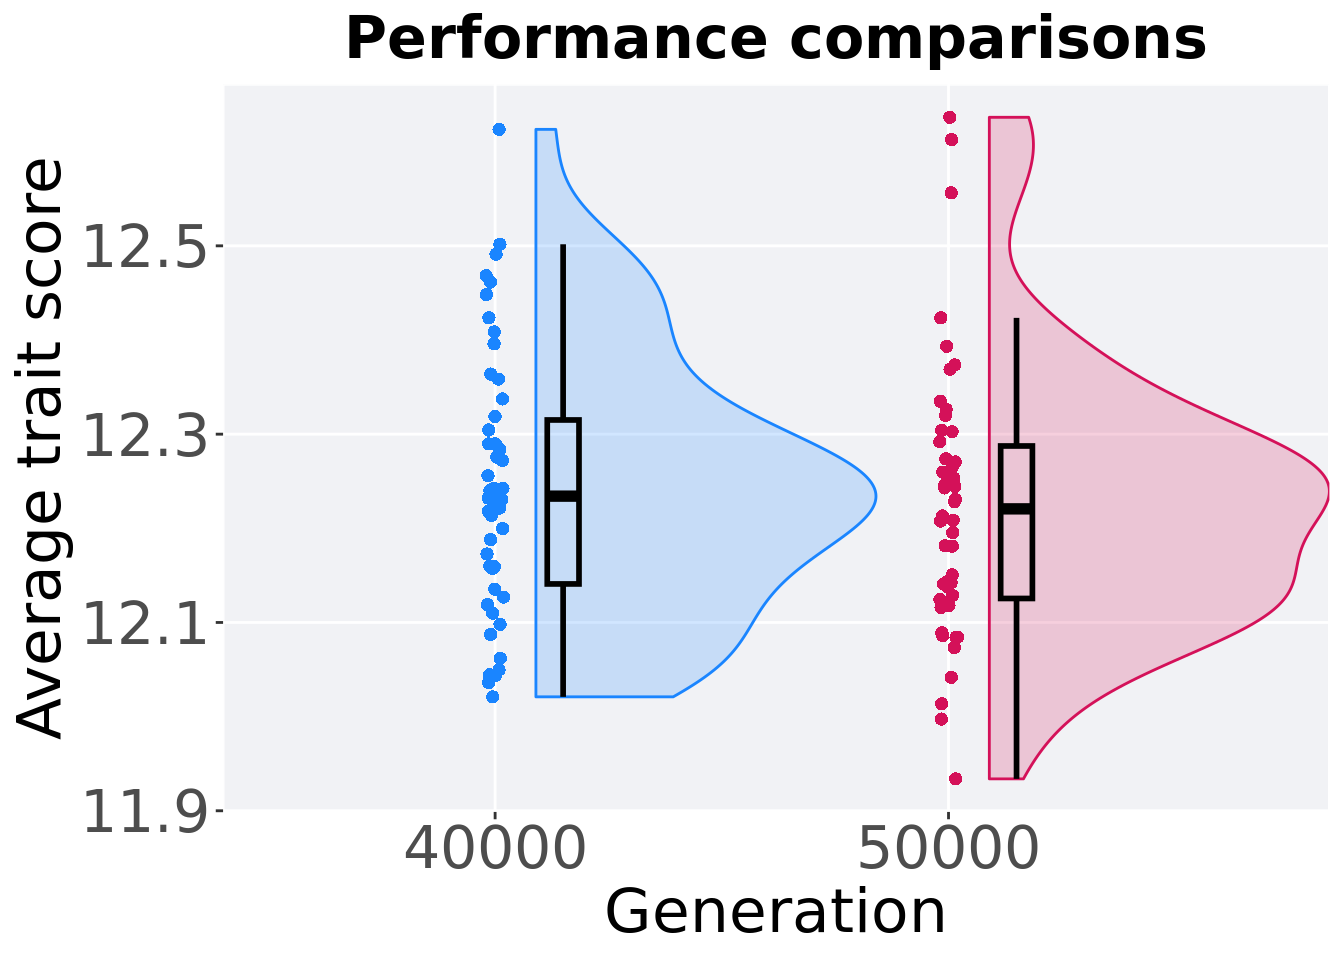
\includegraphics{mvc-diagnostics_files/figure-latex/exp-per-cmp-plt-lex-1.pdf}

Summary statistics for the best performance.

\begin{Shaded}
\begin{Highlighting}[]
\KeywordTok{filter}\NormalTok{(interval_df, acro }\OperatorTok{==}\StringTok{ 'lex'}\NormalTok{) }\OperatorTok
\StringTok{  }\KeywordTok{group_by}\NormalTok{(Generation) }\OperatorTok
\StringTok{  }\NormalTok{dplyr}\OperatorTok{::}\KeywordTok{summarise}\NormalTok{(}
    \DataTypeTok{count =} \KeywordTok{n}\NormalTok{(),}
    \DataTypeTok{na_cnt =} \KeywordTok{sum}\NormalTok{(}\KeywordTok{is.na}\NormalTok{(pop_fit_max)),}
    \DataTypeTok{min =} \KeywordTok{min}\NormalTok{(pop_fit_max }\OperatorTok{/}\StringTok{ }\NormalTok{DIMENSIONALITY, }\DataTypeTok{na.rm =} \OtherTok{TRUE}\NormalTok{),}
    \DataTypeTok{median =} \KeywordTok{median}\NormalTok{(pop_fit_max }\OperatorTok{/}\StringTok{ }\NormalTok{DIMENSIONALITY, }\DataTypeTok{na.rm =} \OtherTok{TRUE}\NormalTok{),}
    \DataTypeTok{mean =} \KeywordTok{mean}\NormalTok{(pop_fit_max }\OperatorTok{/}\StringTok{ }\NormalTok{DIMENSIONALITY, }\DataTypeTok{na.rm =} \OtherTok{TRUE}\NormalTok{),}
    \DataTypeTok{max =} \KeywordTok{max}\NormalTok{(pop_fit_max }\OperatorTok{/}\StringTok{ }\NormalTok{DIMENSIONALITY, }\DataTypeTok{na.rm =} \OtherTok{TRUE}\NormalTok{),}
    \DataTypeTok{IQR =} \KeywordTok{IQR}\NormalTok{(pop_fit_max }\OperatorTok{/}\StringTok{ }\NormalTok{DIMENSIONALITY, }\DataTypeTok{na.rm =} \OtherTok{TRUE}\NormalTok{)}
\NormalTok{  )}
\end{Highlighting}
\end{Shaded}

\begin{verbatim}
## # A tibble: 2 x 8
##   Generation count na_cnt   min median  mean   max   IQR
##   <fct>      <int>  <int> <dbl>  <dbl> <dbl> <dbl> <dbl>
## 1 40000         50      0  12.0   12.2  12.2  12.6 0.174
## 2 50000         50      0  11.9   12.2  12.2  12.6 0.162
\end{verbatim}

Results for post-hoc Wilcoxon rank-sum test.

\begin{Shaded}
\begin{Highlighting}[]
\KeywordTok{wilcox.test}\NormalTok{(}\DataTypeTok{x =} \KeywordTok{filter}\NormalTok{(interval_df, acro }\OperatorTok{==}\StringTok{ 'lex'} \OperatorTok{&}\StringTok{ }\NormalTok{Generation }\OperatorTok{==}\StringTok{ }\DecValTok{50000}\NormalTok{)}\OperatorTok{$}\NormalTok{pop_fit_max,}
            \DataTypeTok{y =} \KeywordTok{filter}\NormalTok{(interval_df, acro }\OperatorTok{==}\StringTok{ 'lex'} \OperatorTok{&}\StringTok{ }\NormalTok{Generation }\OperatorTok{==}\StringTok{ }\DecValTok{40000}\NormalTok{)}\OperatorTok{$}\NormalTok{pop_fit_max,}
            \DataTypeTok{alternative =} \StringTok{'t'}\NormalTok{)}
\end{Highlighting}
\end{Shaded}

\begin{verbatim}
## 
##  Wilcoxon rank sum test with continuity correction
## 
## data:  filter(interval_df, acro == "lex" & Generation == 50000)$pop_fit_max and filter(interval_df, acro == "lex" & Generation == 40000)$pop_fit_max
## W = 1155, p-value = 0.5147
## alternative hypothesis: true location shift is not equal to 0
\end{verbatim}

\hypertarget{genotypic-fitness-sharing}{%
\subsubsection{Genotypic fitness sharing}\label{genotypic-fitness-sharing}}

Plot for comparing performances at interval 40,000 \& 50,000.

\begin{Shaded}
\begin{Highlighting}[]
\KeywordTok{filter}\NormalTok{(interval_df, acro }\OperatorTok{==}\StringTok{ 'gfs'}\NormalTok{) }\OperatorTok
\KeywordTok{ggplot}\NormalTok{(., }\KeywordTok{aes}\NormalTok{(}\DataTypeTok{x=}\NormalTok{Generation, }\DataTypeTok{y=}\NormalTok{pop_fit_max}\OperatorTok{/}\NormalTok{DIMENSIONALITY,}\DataTypeTok{fill=}\NormalTok{Generation,}\DataTypeTok{color=}\NormalTok{Generation,}\DataTypeTok{shape=}\NormalTok{Generation)) }\OperatorTok{+}
\StringTok{  }\KeywordTok{geom_flat_violin}\NormalTok{(}\DataTypeTok{position =} \KeywordTok{position_nudge}\NormalTok{(}\DataTypeTok{x =} \FloatTok{.09}\NormalTok{, }\DataTypeTok{y =} \DecValTok{0}\NormalTok{), }\DataTypeTok{scale =} \StringTok{'width'}\NormalTok{, }\DataTypeTok{alpha =} \FloatTok{0.2}\NormalTok{, }\DataTypeTok{width =} \FloatTok{1.5}\NormalTok{) }\OperatorTok{+}
\StringTok{  }\KeywordTok{geom_boxplot}\NormalTok{(}\DataTypeTok{color =} \StringTok{'black'}\NormalTok{, }\DataTypeTok{width =} \FloatTok{.07}\NormalTok{, }\DataTypeTok{outlier.shape =} \OtherTok{NA}\NormalTok{, }\DataTypeTok{alpha =} \FloatTok{0.0}\NormalTok{, }\DataTypeTok{size =} \FloatTok{1.0}\NormalTok{, }\DataTypeTok{position =} \KeywordTok{position_nudge}\NormalTok{(}\DataTypeTok{x =} \FloatTok{.15}\NormalTok{, }\DataTypeTok{y =} \DecValTok{0}\NormalTok{)) }\OperatorTok{+}
\StringTok{  }\KeywordTok{geom_point}\NormalTok{(}\DataTypeTok{position =} \KeywordTok{position_jitter}\NormalTok{(}\DataTypeTok{width =} \FloatTok{.02}\NormalTok{), }\DataTypeTok{size =} \FloatTok{2.0}\NormalTok{, }\DataTypeTok{alpha =} \FloatTok{1.0}\NormalTok{) }\OperatorTok{+}
\StringTok{    }\KeywordTok{scale_y_continuous}\NormalTok{(}
      \DataTypeTok{name=}\StringTok{"Average trait score"}\NormalTok{,}
\NormalTok{    ) }\OperatorTok{+}
\StringTok{    }\KeywordTok{scale_x_discrete}\NormalTok{(}
      \DataTypeTok{name=}\StringTok{"Generation"}
\NormalTok{    ) }\OperatorTok{+}
\StringTok{  }\KeywordTok{scale_shape_manual}\NormalTok{(}\DataTypeTok{values=}\KeywordTok{c}\NormalTok{(}\DecValTok{16}\NormalTok{,}\DecValTok{16}\NormalTok{))}\OperatorTok{+}
\StringTok{  }\KeywordTok{scale_colour_manual}\NormalTok{(}\DataTypeTok{values =}\NormalTok{ mvc_col, ) }\OperatorTok{+}
\StringTok{  }\KeywordTok{scale_fill_manual}\NormalTok{(}\DataTypeTok{values =}\NormalTok{ mvc_col) }\OperatorTok{+}
\StringTok{  }\KeywordTok{ggtitle}\NormalTok{(}\StringTok{'Performance comparisons'}\NormalTok{)}\OperatorTok{+}
\StringTok{  }\NormalTok{p_theme }\OperatorTok{+}\StringTok{ }\KeywordTok{theme}\NormalTok{(}\DataTypeTok{legend.position=}\StringTok{"none"}\NormalTok{)}
\end{Highlighting}
\end{Shaded}

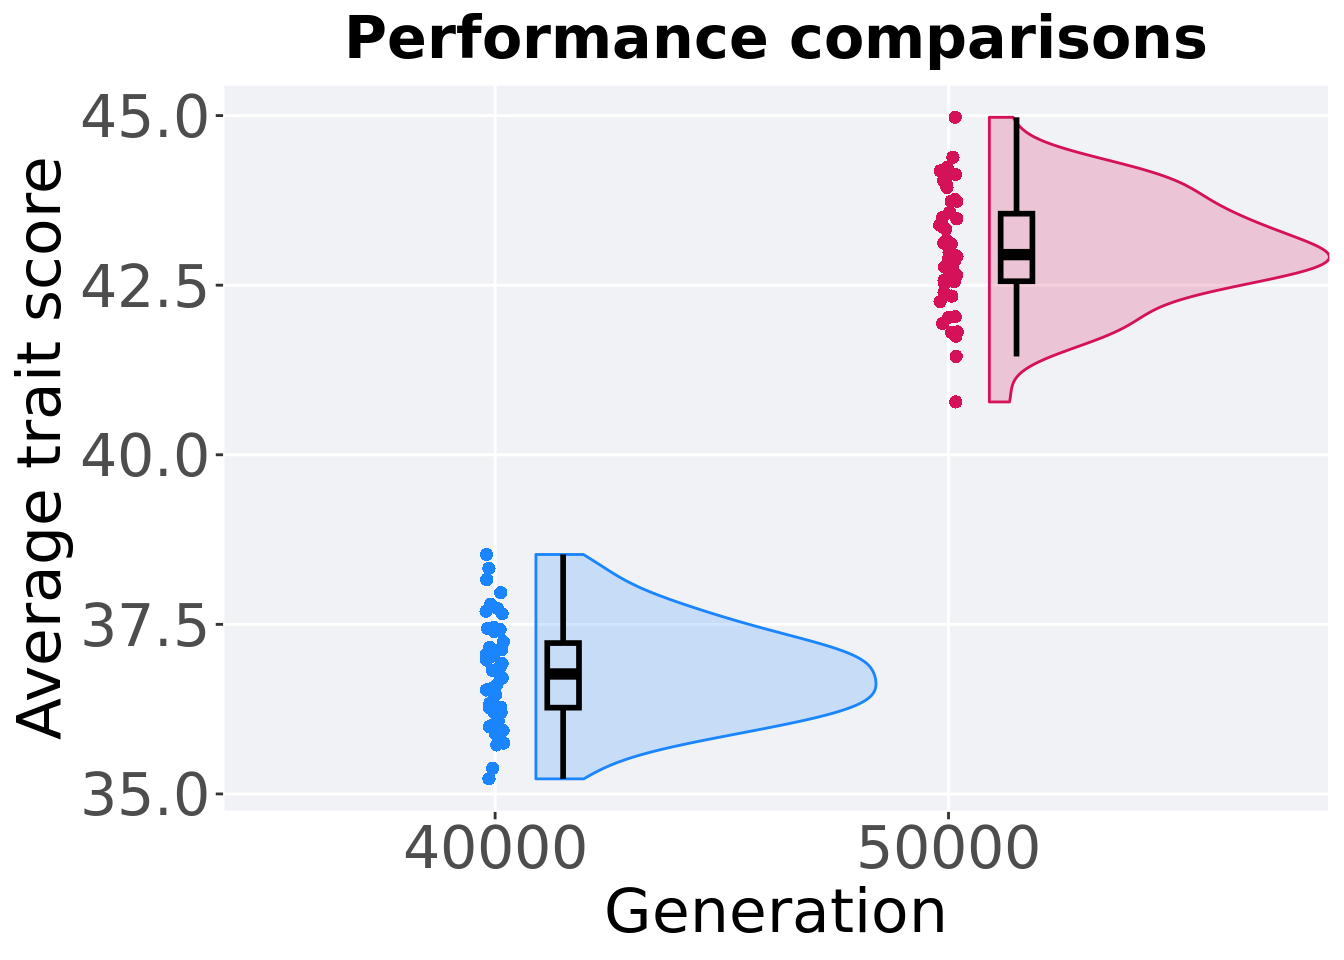
\includegraphics{mvc-diagnostics_files/figure-latex/exp-per-cmp-plt-gfs-1.pdf}

Summary statistics for the best performance.

\begin{Shaded}
\begin{Highlighting}[]
\KeywordTok{filter}\NormalTok{(interval_df, acro }\OperatorTok{==}\StringTok{ 'gfs'}\NormalTok{) }\OperatorTok
\StringTok{  }\KeywordTok{group_by}\NormalTok{(Generation) }\OperatorTok
\StringTok{  }\NormalTok{dplyr}\OperatorTok{::}\KeywordTok{summarise}\NormalTok{(}
    \DataTypeTok{count =} \KeywordTok{n}\NormalTok{(),}
    \DataTypeTok{na_cnt =} \KeywordTok{sum}\NormalTok{(}\KeywordTok{is.na}\NormalTok{(pop_fit_max)),}
    \DataTypeTok{min =} \KeywordTok{min}\NormalTok{(pop_fit_max }\OperatorTok{/}\StringTok{ }\NormalTok{DIMENSIONALITY, }\DataTypeTok{na.rm =} \OtherTok{TRUE}\NormalTok{),}
    \DataTypeTok{median =} \KeywordTok{median}\NormalTok{(pop_fit_max }\OperatorTok{/}\StringTok{ }\NormalTok{DIMENSIONALITY, }\DataTypeTok{na.rm =} \OtherTok{TRUE}\NormalTok{),}
    \DataTypeTok{mean =} \KeywordTok{mean}\NormalTok{(pop_fit_max }\OperatorTok{/}\StringTok{ }\NormalTok{DIMENSIONALITY, }\DataTypeTok{na.rm =} \OtherTok{TRUE}\NormalTok{),}
    \DataTypeTok{max =} \KeywordTok{max}\NormalTok{(pop_fit_max }\OperatorTok{/}\StringTok{ }\NormalTok{DIMENSIONALITY, }\DataTypeTok{na.rm =} \OtherTok{TRUE}\NormalTok{),}
    \DataTypeTok{IQR =} \KeywordTok{IQR}\NormalTok{(pop_fit_max }\OperatorTok{/}\StringTok{ }\NormalTok{DIMENSIONALITY, }\DataTypeTok{na.rm =} \OtherTok{TRUE}\NormalTok{)}
\NormalTok{  )}
\end{Highlighting}
\end{Shaded}

\begin{verbatim}
## # A tibble: 2 x 8
##   Generation count na_cnt   min median  mean   max   IQR
##   <fct>      <int>  <int> <dbl>  <dbl> <dbl> <dbl> <dbl>
## 1 40000         50      0  35.2   36.8  36.8  38.5 0.952
## 2 50000         50      0  40.8   43.0  43.0  45.0 0.996
\end{verbatim}

Results for post-hoc Wilcoxon rank-sum test.

\begin{Shaded}
\begin{Highlighting}[]
\KeywordTok{wilcox.test}\NormalTok{(}\DataTypeTok{x =} \KeywordTok{filter}\NormalTok{(interval_df, acro }\OperatorTok{==}\StringTok{ 'gfs'} \OperatorTok{&}\StringTok{ }\NormalTok{Generation }\OperatorTok{==}\StringTok{ }\DecValTok{50000}\NormalTok{)}\OperatorTok{$}\NormalTok{pop_fit_max,}
            \DataTypeTok{y =} \KeywordTok{filter}\NormalTok{(interval_df, acro }\OperatorTok{==}\StringTok{ 'gfs'} \OperatorTok{&}\StringTok{ }\NormalTok{Generation }\OperatorTok{==}\StringTok{ }\DecValTok{40000}\NormalTok{)}\OperatorTok{$}\NormalTok{pop_fit_max,}
            \DataTypeTok{alternative =} \StringTok{'g'}\NormalTok{)}
\end{Highlighting}
\end{Shaded}

\begin{verbatim}
## 
##  Wilcoxon rank sum test with continuity correction
## 
## data:  filter(interval_df, acro == "gfs" & Generation == 50000)$pop_fit_max and filter(interval_df, acro == "gfs" & Generation == 40000)$pop_fit_max
## W = 2500, p-value < 2.2e-16
## alternative hypothesis: true location shift is greater than 0
\end{verbatim}

\hypertarget{phenotypic-fitness-sharing}{%
\subsubsection{Phenotypic fitness sharing}\label{phenotypic-fitness-sharing}}

Plot for comparing performances at interval 40,000 \& 50,000.

\begin{Shaded}
\begin{Highlighting}[]
\KeywordTok{filter}\NormalTok{(interval_df, acro }\OperatorTok{==}\StringTok{ 'pfs'}\NormalTok{) }\OperatorTok
\KeywordTok{ggplot}\NormalTok{(., }\KeywordTok{aes}\NormalTok{(}\DataTypeTok{x=}\NormalTok{Generation, }\DataTypeTok{y=}\NormalTok{pop_fit_max}\OperatorTok{/}\NormalTok{DIMENSIONALITY,}\DataTypeTok{fill=}\NormalTok{Generation,}\DataTypeTok{color=}\NormalTok{Generation,}\DataTypeTok{shape=}\NormalTok{Generation)) }\OperatorTok{+}
\StringTok{  }\KeywordTok{geom_flat_violin}\NormalTok{(}\DataTypeTok{position =} \KeywordTok{position_nudge}\NormalTok{(}\DataTypeTok{x =} \FloatTok{.09}\NormalTok{, }\DataTypeTok{y =} \DecValTok{0}\NormalTok{), }\DataTypeTok{scale =} \StringTok{'width'}\NormalTok{, }\DataTypeTok{alpha =} \FloatTok{0.2}\NormalTok{, }\DataTypeTok{width =} \FloatTok{1.5}\NormalTok{) }\OperatorTok{+}
\StringTok{  }\KeywordTok{geom_boxplot}\NormalTok{(}\DataTypeTok{color =} \StringTok{'black'}\NormalTok{, }\DataTypeTok{width =} \FloatTok{.07}\NormalTok{, }\DataTypeTok{outlier.shape =} \OtherTok{NA}\NormalTok{, }\DataTypeTok{alpha =} \FloatTok{0.0}\NormalTok{, }\DataTypeTok{size =} \FloatTok{1.0}\NormalTok{, }\DataTypeTok{position =} \KeywordTok{position_nudge}\NormalTok{(}\DataTypeTok{x =} \FloatTok{.15}\NormalTok{, }\DataTypeTok{y =} \DecValTok{0}\NormalTok{)) }\OperatorTok{+}
\StringTok{  }\KeywordTok{geom_point}\NormalTok{(}\DataTypeTok{position =} \KeywordTok{position_jitter}\NormalTok{(}\DataTypeTok{width =} \FloatTok{.02}\NormalTok{), }\DataTypeTok{size =} \FloatTok{2.0}\NormalTok{, }\DataTypeTok{alpha =} \FloatTok{1.0}\NormalTok{) }\OperatorTok{+}
\StringTok{    }\KeywordTok{scale_y_continuous}\NormalTok{(}
      \DataTypeTok{name=}\StringTok{"Average trait score"}\NormalTok{,}
\NormalTok{    ) }\OperatorTok{+}
\StringTok{    }\KeywordTok{scale_x_discrete}\NormalTok{(}
      \DataTypeTok{name=}\StringTok{"Generation"}
\NormalTok{    ) }\OperatorTok{+}
\StringTok{  }\KeywordTok{scale_shape_manual}\NormalTok{(}\DataTypeTok{values=}\KeywordTok{c}\NormalTok{(}\DecValTok{16}\NormalTok{,}\DecValTok{16}\NormalTok{))}\OperatorTok{+}
\StringTok{  }\KeywordTok{scale_colour_manual}\NormalTok{(}\DataTypeTok{values =}\NormalTok{ mvc_col, ) }\OperatorTok{+}
\StringTok{  }\KeywordTok{scale_fill_manual}\NormalTok{(}\DataTypeTok{values =}\NormalTok{ mvc_col) }\OperatorTok{+}
\StringTok{  }\KeywordTok{ggtitle}\NormalTok{(}\StringTok{'Performance comparisons'}\NormalTok{)}\OperatorTok{+}
\StringTok{  }\NormalTok{p_theme }\OperatorTok{+}\StringTok{ }\KeywordTok{theme}\NormalTok{(}\DataTypeTok{legend.position=}\StringTok{"none"}\NormalTok{)}
\end{Highlighting}
\end{Shaded}

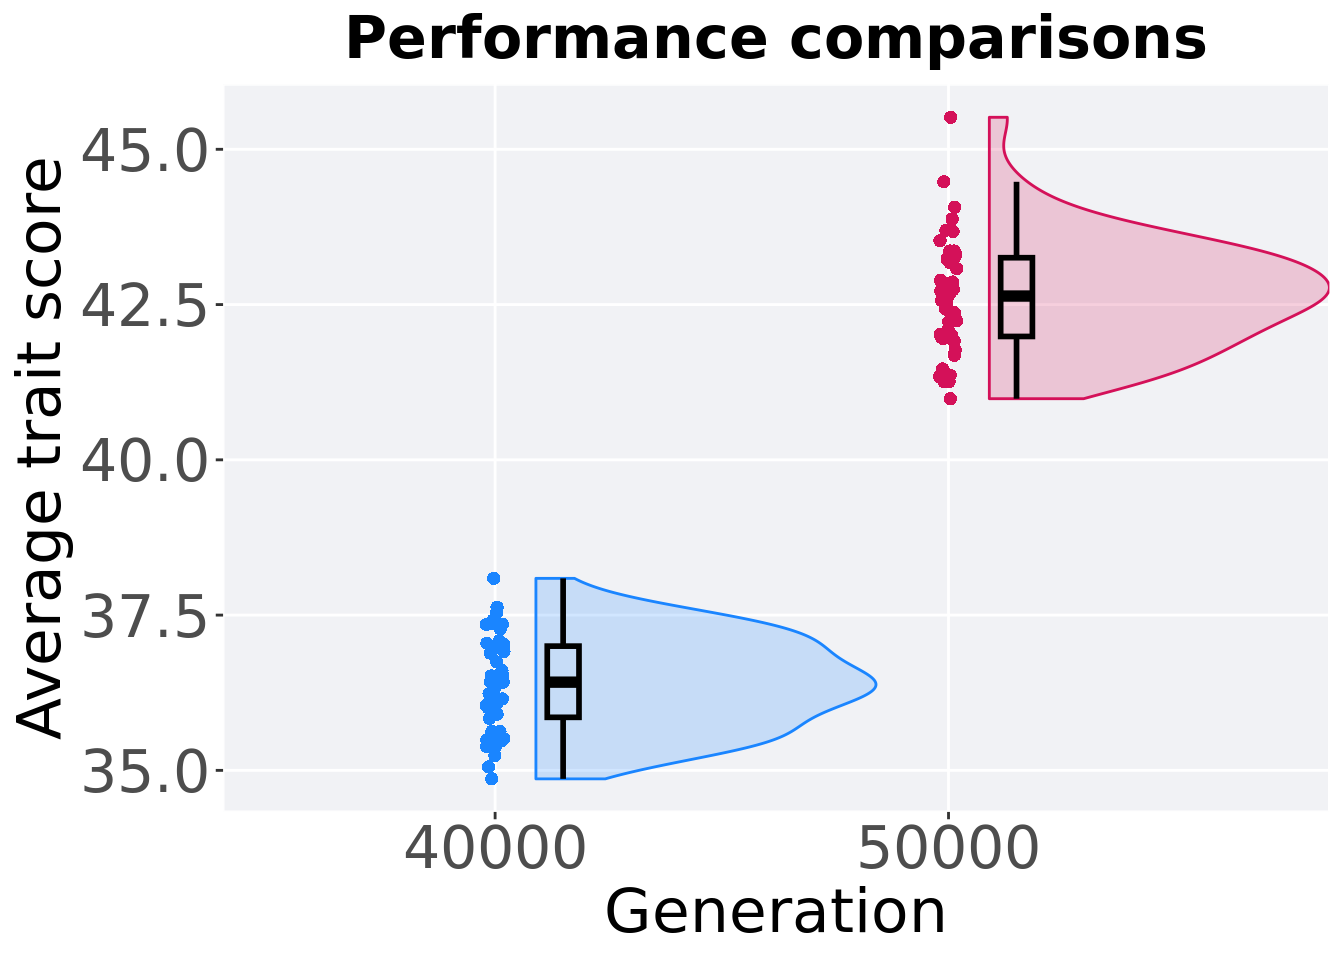
\includegraphics{mvc-diagnostics_files/figure-latex/exp-per-cmp-plt-pfs-1.pdf}

Summary statistics for the best performance.

\begin{Shaded}
\begin{Highlighting}[]
\KeywordTok{filter}\NormalTok{(interval_df, acro }\OperatorTok{==}\StringTok{ 'pfs'}\NormalTok{) }\OperatorTok
\StringTok{  }\KeywordTok{group_by}\NormalTok{(Generation) }\OperatorTok
\StringTok{  }\NormalTok{dplyr}\OperatorTok{::}\KeywordTok{summarise}\NormalTok{(}
    \DataTypeTok{count =} \KeywordTok{n}\NormalTok{(),}
    \DataTypeTok{na_cnt =} \KeywordTok{sum}\NormalTok{(}\KeywordTok{is.na}\NormalTok{(pop_fit_max)),}
    \DataTypeTok{min =} \KeywordTok{min}\NormalTok{(pop_fit_max }\OperatorTok{/}\StringTok{ }\NormalTok{DIMENSIONALITY, }\DataTypeTok{na.rm =} \OtherTok{TRUE}\NormalTok{),}
    \DataTypeTok{median =} \KeywordTok{median}\NormalTok{(pop_fit_max }\OperatorTok{/}\StringTok{ }\NormalTok{DIMENSIONALITY, }\DataTypeTok{na.rm =} \OtherTok{TRUE}\NormalTok{),}
    \DataTypeTok{mean =} \KeywordTok{mean}\NormalTok{(pop_fit_max }\OperatorTok{/}\StringTok{ }\NormalTok{DIMENSIONALITY, }\DataTypeTok{na.rm =} \OtherTok{TRUE}\NormalTok{),}
    \DataTypeTok{max =} \KeywordTok{max}\NormalTok{(pop_fit_max }\OperatorTok{/}\StringTok{ }\NormalTok{DIMENSIONALITY, }\DataTypeTok{na.rm =} \OtherTok{TRUE}\NormalTok{),}
    \DataTypeTok{IQR =} \KeywordTok{IQR}\NormalTok{(pop_fit_max }\OperatorTok{/}\StringTok{ }\NormalTok{DIMENSIONALITY, }\DataTypeTok{na.rm =} \OtherTok{TRUE}\NormalTok{)}
\NormalTok{  )}
\end{Highlighting}
\end{Shaded}

\begin{verbatim}
## # A tibble: 2 x 8
##   Generation count na_cnt   min median  mean   max   IQR
##   <fct>      <int>  <int> <dbl>  <dbl> <dbl> <dbl> <dbl>
## 1 40000         50      0  34.9   36.4  36.4  38.1  1.15
## 2 50000         50      0  41.0   42.6  42.6  45.5  1.27
\end{verbatim}

Results for post-hoc Wilcoxon rank-sum test.

\begin{Shaded}
\begin{Highlighting}[]
\KeywordTok{wilcox.test}\NormalTok{(}\DataTypeTok{x =} \KeywordTok{filter}\NormalTok{(interval_df, acro }\OperatorTok{==}\StringTok{ 'pfs'} \OperatorTok{&}\StringTok{ }\NormalTok{Generation }\OperatorTok{==}\StringTok{ }\DecValTok{50000}\NormalTok{)}\OperatorTok{$}\NormalTok{pop_fit_max,}
            \DataTypeTok{y =} \KeywordTok{filter}\NormalTok{(interval_df, acro }\OperatorTok{==}\StringTok{ 'pfs'} \OperatorTok{&}\StringTok{ }\NormalTok{Generation }\OperatorTok{==}\StringTok{ }\DecValTok{40000}\NormalTok{)}\OperatorTok{$}\NormalTok{pop_fit_max,}
            \DataTypeTok{alternative =} \StringTok{'g'}\NormalTok{)}
\end{Highlighting}
\end{Shaded}

\begin{verbatim}
## 
##  Wilcoxon rank sum test with continuity correction
## 
## data:  filter(interval_df, acro == "pfs" & Generation == 50000)$pop_fit_max and filter(interval_df, acro == "pfs" & Generation == 40000)$pop_fit_max
## W = 2500, p-value < 2.2e-16
## alternative hypothesis: true location shift is greater than 0
\end{verbatim}

\hypertarget{nondominated-sorting}{%
\subsubsection{Nondominated sorting}\label{nondominated-sorting}}

Plot for comparing performances at interval 40,000 \& 50,000.

\begin{Shaded}
\begin{Highlighting}[]
\KeywordTok{filter}\NormalTok{(interval_df, acro }\OperatorTok{==}\StringTok{ 'nds'}\NormalTok{) }\OperatorTok
\KeywordTok{ggplot}\NormalTok{(., }\KeywordTok{aes}\NormalTok{(}\DataTypeTok{x=}\NormalTok{Generation, }\DataTypeTok{y=}\NormalTok{pop_fit_max}\OperatorTok{/}\NormalTok{DIMENSIONALITY,}\DataTypeTok{fill=}\NormalTok{Generation,}\DataTypeTok{color=}\NormalTok{Generation,}\DataTypeTok{shape=}\NormalTok{Generation)) }\OperatorTok{+}
\StringTok{  }\KeywordTok{geom_flat_violin}\NormalTok{(}\DataTypeTok{position =} \KeywordTok{position_nudge}\NormalTok{(}\DataTypeTok{x =} \FloatTok{.09}\NormalTok{, }\DataTypeTok{y =} \DecValTok{0}\NormalTok{), }\DataTypeTok{scale =} \StringTok{'width'}\NormalTok{, }\DataTypeTok{alpha =} \FloatTok{0.2}\NormalTok{, }\DataTypeTok{width =} \FloatTok{1.5}\NormalTok{) }\OperatorTok{+}
\StringTok{  }\KeywordTok{geom_boxplot}\NormalTok{(}\DataTypeTok{color =} \StringTok{'black'}\NormalTok{, }\DataTypeTok{width =} \FloatTok{.07}\NormalTok{, }\DataTypeTok{outlier.shape =} \OtherTok{NA}\NormalTok{, }\DataTypeTok{alpha =} \FloatTok{0.0}\NormalTok{, }\DataTypeTok{size =} \FloatTok{1.0}\NormalTok{, }\DataTypeTok{position =} \KeywordTok{position_nudge}\NormalTok{(}\DataTypeTok{x =} \FloatTok{.15}\NormalTok{, }\DataTypeTok{y =} \DecValTok{0}\NormalTok{)) }\OperatorTok{+}
\StringTok{  }\KeywordTok{geom_point}\NormalTok{(}\DataTypeTok{position =} \KeywordTok{position_jitter}\NormalTok{(}\DataTypeTok{width =} \FloatTok{.02}\NormalTok{), }\DataTypeTok{size =} \FloatTok{2.0}\NormalTok{, }\DataTypeTok{alpha =} \FloatTok{1.0}\NormalTok{) }\OperatorTok{+}
\StringTok{    }\KeywordTok{scale_y_continuous}\NormalTok{(}
      \DataTypeTok{name=}\StringTok{"Average trait score"}\NormalTok{,}
\NormalTok{    ) }\OperatorTok{+}
\StringTok{    }\KeywordTok{scale_x_discrete}\NormalTok{(}
      \DataTypeTok{name=}\StringTok{"Generation"}
\NormalTok{    ) }\OperatorTok{+}
\StringTok{  }\KeywordTok{scale_shape_manual}\NormalTok{(}\DataTypeTok{values=}\KeywordTok{c}\NormalTok{(}\DecValTok{16}\NormalTok{,}\DecValTok{16}\NormalTok{))}\OperatorTok{+}
\StringTok{  }\KeywordTok{scale_colour_manual}\NormalTok{(}\DataTypeTok{values =}\NormalTok{ mvc_col, ) }\OperatorTok{+}
\StringTok{  }\KeywordTok{scale_fill_manual}\NormalTok{(}\DataTypeTok{values =}\NormalTok{ mvc_col) }\OperatorTok{+}
\StringTok{  }\KeywordTok{ggtitle}\NormalTok{(}\StringTok{'Performance comparisons'}\NormalTok{)}\OperatorTok{+}
\StringTok{  }\NormalTok{p_theme }\OperatorTok{+}\StringTok{ }\KeywordTok{theme}\NormalTok{(}\DataTypeTok{legend.position=}\StringTok{"none"}\NormalTok{)}
\end{Highlighting}
\end{Shaded}

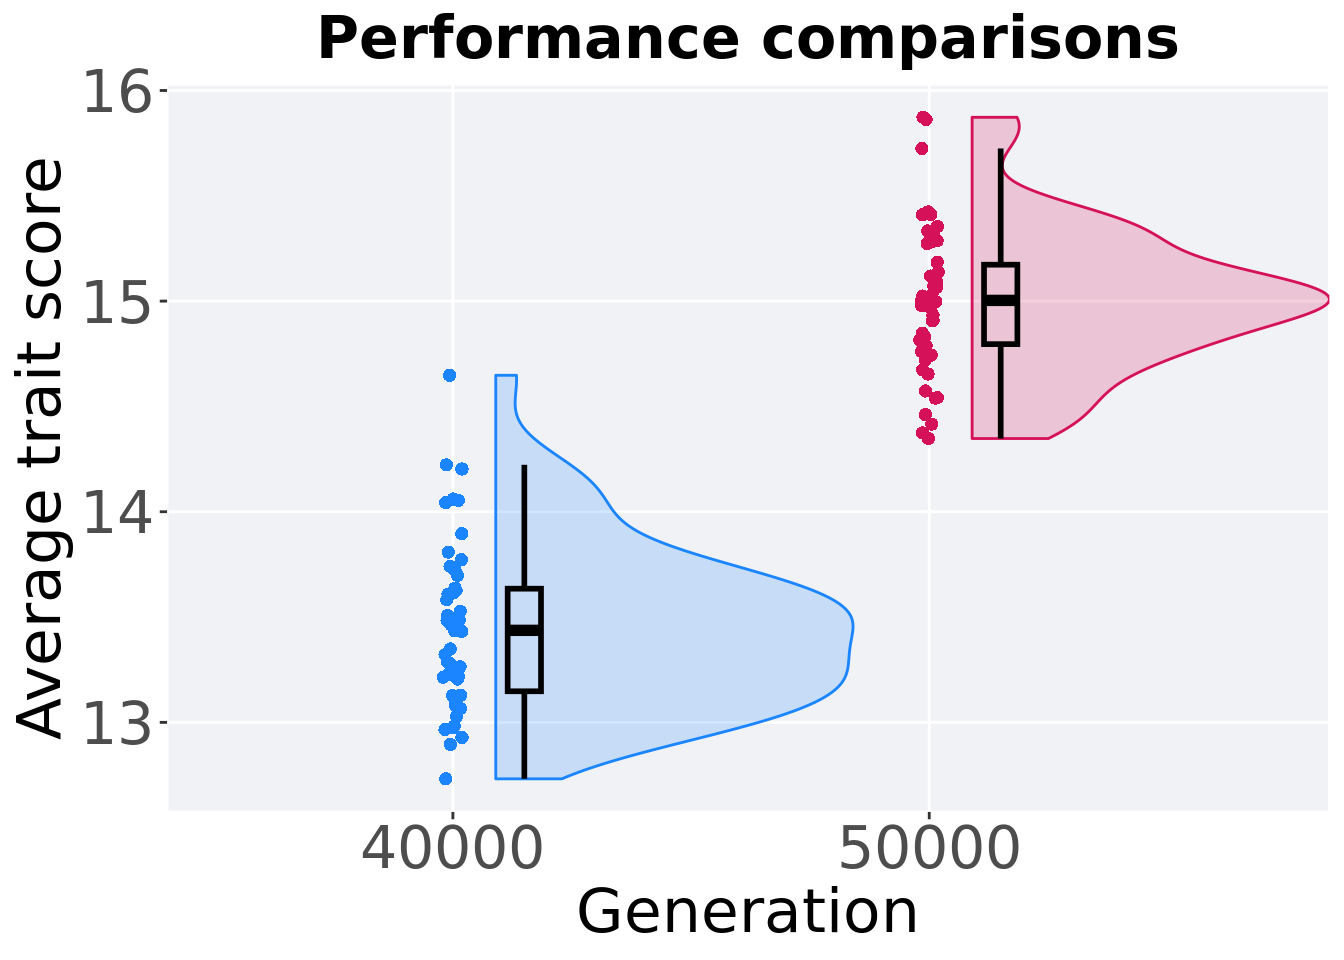
\includegraphics{mvc-diagnostics_files/figure-latex/exp-per-cmp-plt-nds-1.pdf}

Summary statistics for the best performance.

\begin{Shaded}
\begin{Highlighting}[]
\KeywordTok{filter}\NormalTok{(interval_df, acro }\OperatorTok{==}\StringTok{ 'nds'}\NormalTok{) }\OperatorTok
\StringTok{  }\KeywordTok{group_by}\NormalTok{(Generation) }\OperatorTok
\StringTok{  }\NormalTok{dplyr}\OperatorTok{::}\KeywordTok{summarise}\NormalTok{(}
    \DataTypeTok{count =} \KeywordTok{n}\NormalTok{(),}
    \DataTypeTok{na_cnt =} \KeywordTok{sum}\NormalTok{(}\KeywordTok{is.na}\NormalTok{(pop_fit_max)),}
    \DataTypeTok{min =} \KeywordTok{min}\NormalTok{(pop_fit_max }\OperatorTok{/}\StringTok{ }\NormalTok{DIMENSIONALITY, }\DataTypeTok{na.rm =} \OtherTok{TRUE}\NormalTok{),}
    \DataTypeTok{median =} \KeywordTok{median}\NormalTok{(pop_fit_max }\OperatorTok{/}\StringTok{ }\NormalTok{DIMENSIONALITY, }\DataTypeTok{na.rm =} \OtherTok{TRUE}\NormalTok{),}
    \DataTypeTok{mean =} \KeywordTok{mean}\NormalTok{(pop_fit_max }\OperatorTok{/}\StringTok{ }\NormalTok{DIMENSIONALITY, }\DataTypeTok{na.rm =} \OtherTok{TRUE}\NormalTok{),}
    \DataTypeTok{max =} \KeywordTok{max}\NormalTok{(pop_fit_max }\OperatorTok{/}\StringTok{ }\NormalTok{DIMENSIONALITY, }\DataTypeTok{na.rm =} \OtherTok{TRUE}\NormalTok{),}
    \DataTypeTok{IQR =} \KeywordTok{IQR}\NormalTok{(pop_fit_max }\OperatorTok{/}\StringTok{ }\NormalTok{DIMENSIONALITY, }\DataTypeTok{na.rm =} \OtherTok{TRUE}\NormalTok{)}
\NormalTok{  )}
\end{Highlighting}
\end{Shaded}

\begin{verbatim}
## # A tibble: 2 x 8
##   Generation count na_cnt   min median  mean   max   IQR
##   <fct>      <int>  <int> <dbl>  <dbl> <dbl> <dbl> <dbl>
## 1 40000         50      0  12.7   13.4  13.5  14.6 0.487
## 2 50000         50      0  14.3   15.0  15.0  15.9 0.377
\end{verbatim}

Results for post-hoc Wilcoxon rank-sum test.

\begin{Shaded}
\begin{Highlighting}[]
\KeywordTok{wilcox.test}\NormalTok{(}\DataTypeTok{x =} \KeywordTok{filter}\NormalTok{(interval_df, acro }\OperatorTok{==}\StringTok{ 'nds'} \OperatorTok{&}\StringTok{ }\NormalTok{Generation }\OperatorTok{==}\StringTok{ }\DecValTok{50000}\NormalTok{)}\OperatorTok{$}\NormalTok{pop_fit_max,}
            \DataTypeTok{y =} \KeywordTok{filter}\NormalTok{(interval_df, acro }\OperatorTok{==}\StringTok{ 'nds'} \OperatorTok{&}\StringTok{ }\NormalTok{Generation }\OperatorTok{==}\StringTok{ }\DecValTok{40000}\NormalTok{)}\OperatorTok{$}\NormalTok{pop_fit_max,}
            \DataTypeTok{alternative =} \StringTok{'g'}\NormalTok{)}
\end{Highlighting}
\end{Shaded}

\begin{verbatim}
## 
##  Wilcoxon rank sum test with continuity correction
## 
## data:  filter(interval_df, acro == "nds" & Generation == 50000)$pop_fit_max and filter(interval_df, acro == "nds" & Generation == 40000)$pop_fit_max
## W = 2493, p-value < 2.2e-16
## alternative hypothesis: true location shift is greater than 0
\end{verbatim}

\hypertarget{novelty-search}{%
\subsubsection{Novelty search}\label{novelty-search}}

Plot for comparing performances at interval 40,000 \& 50,000.

\begin{Shaded}
\begin{Highlighting}[]
\KeywordTok{filter}\NormalTok{(interval_df, acro }\OperatorTok{==}\StringTok{ 'nov'}\NormalTok{) }\OperatorTok
\KeywordTok{ggplot}\NormalTok{(., }\KeywordTok{aes}\NormalTok{(}\DataTypeTok{x=}\NormalTok{Generation, }\DataTypeTok{y=}\NormalTok{pop_fit_max}\OperatorTok{/}\NormalTok{DIMENSIONALITY,}\DataTypeTok{fill=}\NormalTok{Generation,}\DataTypeTok{color=}\NormalTok{Generation,}\DataTypeTok{shape=}\NormalTok{Generation)) }\OperatorTok{+}
\StringTok{  }\KeywordTok{geom_flat_violin}\NormalTok{(}\DataTypeTok{position =} \KeywordTok{position_nudge}\NormalTok{(}\DataTypeTok{x =} \FloatTok{.09}\NormalTok{, }\DataTypeTok{y =} \DecValTok{0}\NormalTok{), }\DataTypeTok{scale =} \StringTok{'width'}\NormalTok{, }\DataTypeTok{alpha =} \FloatTok{0.2}\NormalTok{, }\DataTypeTok{width =} \FloatTok{1.5}\NormalTok{) }\OperatorTok{+}
\StringTok{  }\KeywordTok{geom_boxplot}\NormalTok{(}\DataTypeTok{color =} \StringTok{'black'}\NormalTok{, }\DataTypeTok{width =} \FloatTok{.07}\NormalTok{, }\DataTypeTok{outlier.shape =} \OtherTok{NA}\NormalTok{, }\DataTypeTok{alpha =} \FloatTok{0.0}\NormalTok{, }\DataTypeTok{size =} \FloatTok{1.0}\NormalTok{, }\DataTypeTok{position =} \KeywordTok{position_nudge}\NormalTok{(}\DataTypeTok{x =} \FloatTok{.15}\NormalTok{, }\DataTypeTok{y =} \DecValTok{0}\NormalTok{)) }\OperatorTok{+}
\StringTok{  }\KeywordTok{geom_point}\NormalTok{(}\DataTypeTok{position =} \KeywordTok{position_jitter}\NormalTok{(}\DataTypeTok{width =} \FloatTok{.02}\NormalTok{), }\DataTypeTok{size =} \FloatTok{2.0}\NormalTok{, }\DataTypeTok{alpha =} \FloatTok{1.0}\NormalTok{) }\OperatorTok{+}
\StringTok{    }\KeywordTok{scale_y_continuous}\NormalTok{(}
      \DataTypeTok{name=}\StringTok{"Average trait score"}\NormalTok{,}
\NormalTok{    ) }\OperatorTok{+}
\StringTok{    }\KeywordTok{scale_x_discrete}\NormalTok{(}
      \DataTypeTok{name=}\StringTok{"Generation"}
\NormalTok{    ) }\OperatorTok{+}
\StringTok{  }\KeywordTok{scale_shape_manual}\NormalTok{(}\DataTypeTok{values=}\KeywordTok{c}\NormalTok{(}\DecValTok{16}\NormalTok{,}\DecValTok{16}\NormalTok{))}\OperatorTok{+}
\StringTok{  }\KeywordTok{scale_colour_manual}\NormalTok{(}\DataTypeTok{values =}\NormalTok{ mvc_col, ) }\OperatorTok{+}
\StringTok{  }\KeywordTok{scale_fill_manual}\NormalTok{(}\DataTypeTok{values =}\NormalTok{ mvc_col) }\OperatorTok{+}
\StringTok{  }\KeywordTok{ggtitle}\NormalTok{(}\StringTok{'Performance comparisons'}\NormalTok{)}\OperatorTok{+}
\StringTok{  }\NormalTok{p_theme }\OperatorTok{+}\StringTok{ }\KeywordTok{theme}\NormalTok{(}\DataTypeTok{legend.position=}\StringTok{"none"}\NormalTok{)}
\end{Highlighting}
\end{Shaded}

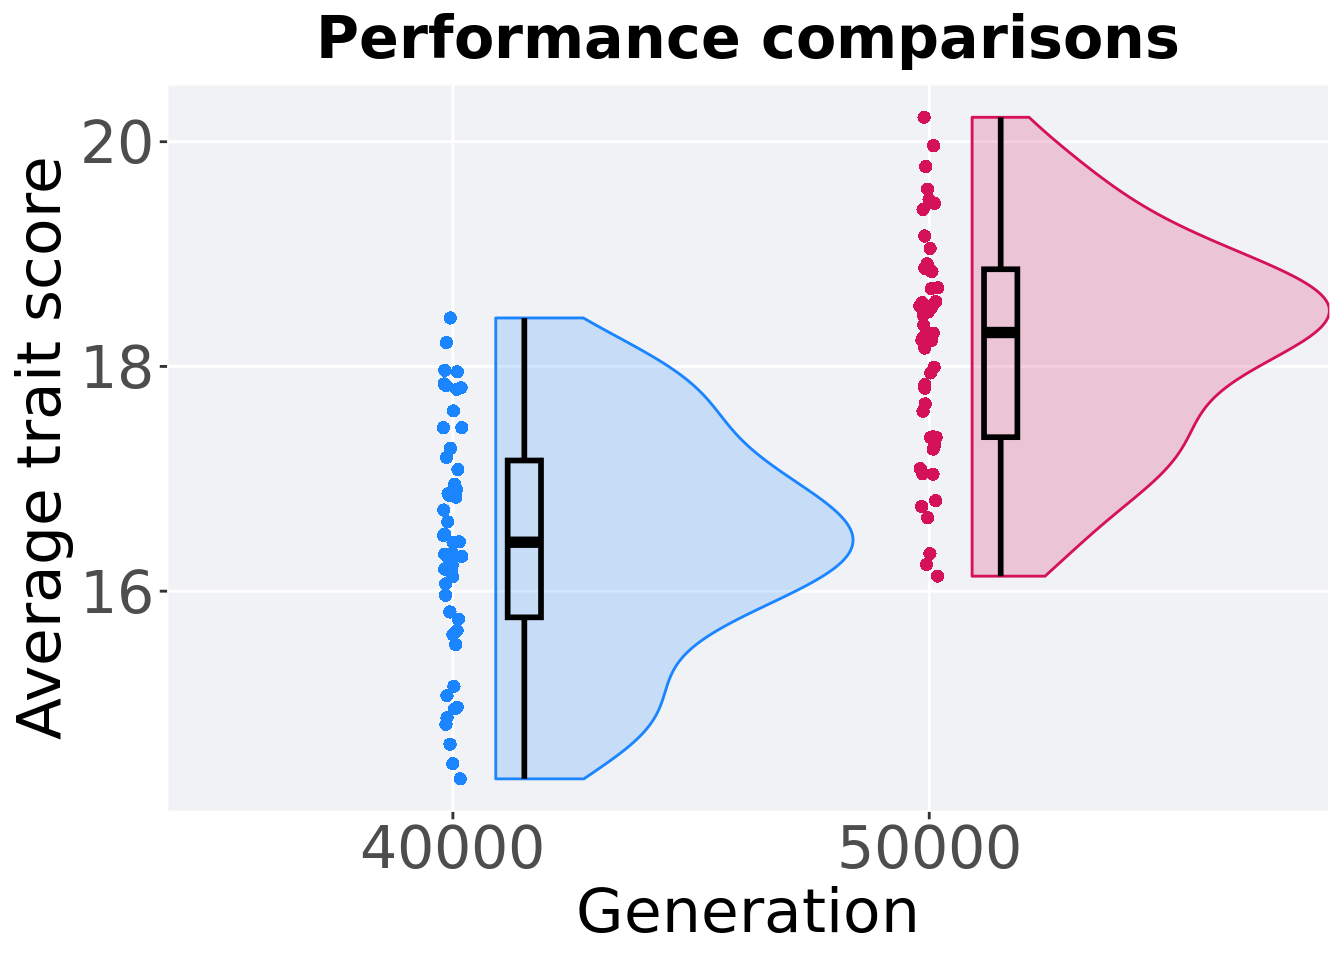
\includegraphics{mvc-diagnostics_files/figure-latex/exp-per-cmp-plt-nov-1.pdf}

Summary statistics for the best performance.

\begin{Shaded}
\begin{Highlighting}[]
\KeywordTok{filter}\NormalTok{(interval_df, acro }\OperatorTok{==}\StringTok{ 'nov'}\NormalTok{) }\OperatorTok
\StringTok{  }\KeywordTok{group_by}\NormalTok{(Generation) }\OperatorTok
\StringTok{  }\NormalTok{dplyr}\OperatorTok{::}\KeywordTok{summarise}\NormalTok{(}
    \DataTypeTok{count =} \KeywordTok{n}\NormalTok{(),}
    \DataTypeTok{na_cnt =} \KeywordTok{sum}\NormalTok{(}\KeywordTok{is.na}\NormalTok{(pop_fit_max)),}
    \DataTypeTok{min =} \KeywordTok{min}\NormalTok{(pop_fit_max }\OperatorTok{/}\StringTok{ }\NormalTok{DIMENSIONALITY, }\DataTypeTok{na.rm =} \OtherTok{TRUE}\NormalTok{),}
    \DataTypeTok{median =} \KeywordTok{median}\NormalTok{(pop_fit_max }\OperatorTok{/}\StringTok{ }\NormalTok{DIMENSIONALITY, }\DataTypeTok{na.rm =} \OtherTok{TRUE}\NormalTok{),}
    \DataTypeTok{mean =} \KeywordTok{mean}\NormalTok{(pop_fit_max }\OperatorTok{/}\StringTok{ }\NormalTok{DIMENSIONALITY, }\DataTypeTok{na.rm =} \OtherTok{TRUE}\NormalTok{),}
    \DataTypeTok{max =} \KeywordTok{max}\NormalTok{(pop_fit_max }\OperatorTok{/}\StringTok{ }\NormalTok{DIMENSIONALITY, }\DataTypeTok{na.rm =} \OtherTok{TRUE}\NormalTok{),}
    \DataTypeTok{IQR =} \KeywordTok{IQR}\NormalTok{(pop_fit_max }\OperatorTok{/}\StringTok{ }\NormalTok{DIMENSIONALITY, }\DataTypeTok{na.rm =} \OtherTok{TRUE}\NormalTok{)}
\NormalTok{  )}
\end{Highlighting}
\end{Shaded}

\begin{verbatim}
## # A tibble: 2 x 8
##   Generation count na_cnt   min median  mean   max   IQR
##   <fct>      <int>  <int> <dbl>  <dbl> <dbl> <dbl> <dbl>
## 1 40000         50      0  14.3   16.4  16.4  18.4  1.40
## 2 50000         50      0  16.1   18.3  18.2  20.2  1.49
\end{verbatim}

Results for post-hoc Wilcoxon rank-sum test.

\begin{Shaded}
\begin{Highlighting}[]
\KeywordTok{wilcox.test}\NormalTok{(}\DataTypeTok{x =} \KeywordTok{filter}\NormalTok{(interval_df, acro }\OperatorTok{==}\StringTok{ 'nov'} \OperatorTok{&}\StringTok{ }\NormalTok{Generation }\OperatorTok{==}\StringTok{ }\DecValTok{50000}\NormalTok{)}\OperatorTok{$}\NormalTok{pop_fit_max,}
            \DataTypeTok{y =} \KeywordTok{filter}\NormalTok{(interval_df, acro }\OperatorTok{==}\StringTok{ 'nov'} \OperatorTok{&}\StringTok{ }\NormalTok{Generation }\OperatorTok{==}\StringTok{ }\DecValTok{40000}\NormalTok{)}\OperatorTok{$}\NormalTok{pop_fit_max,}
            \DataTypeTok{alternative =} \StringTok{'g'}\NormalTok{)}
\end{Highlighting}
\end{Shaded}

\begin{verbatim}
## 
##  Wilcoxon rank sum test with continuity correction
## 
## data:  filter(interval_df, acro == "nov" & Generation == 50000)$pop_fit_max and filter(interval_df, acro == "nov" & Generation == 40000)$pop_fit_max
## W = 2209, p-value = 1.951e-11
## alternative hypothesis: true location shift is greater than 0
\end{verbatim}

\hypertarget{random}{%
\subsubsection{Random}\label{random}}

Plot for comparing performances at interval 40,000 \& 50,000.

\begin{Shaded}
\begin{Highlighting}[]
\KeywordTok{filter}\NormalTok{(interval_df, acro }\OperatorTok{==}\StringTok{ 'ran'}\NormalTok{) }\OperatorTok
\KeywordTok{ggplot}\NormalTok{(., }\KeywordTok{aes}\NormalTok{(}\DataTypeTok{x=}\NormalTok{Generation, }\DataTypeTok{y=}\NormalTok{pop_fit_max}\OperatorTok{/}\NormalTok{DIMENSIONALITY,}\DataTypeTok{fill=}\NormalTok{Generation,}\DataTypeTok{color=}\NormalTok{Generation,}\DataTypeTok{shape=}\NormalTok{Generation)) }\OperatorTok{+}
\StringTok{  }\KeywordTok{geom_flat_violin}\NormalTok{(}\DataTypeTok{position =} \KeywordTok{position_nudge}\NormalTok{(}\DataTypeTok{x =} \FloatTok{.09}\NormalTok{, }\DataTypeTok{y =} \DecValTok{0}\NormalTok{), }\DataTypeTok{scale =} \StringTok{'width'}\NormalTok{, }\DataTypeTok{alpha =} \FloatTok{0.2}\NormalTok{, }\DataTypeTok{width =} \FloatTok{1.5}\NormalTok{) }\OperatorTok{+}
\StringTok{  }\KeywordTok{geom_boxplot}\NormalTok{(}\DataTypeTok{color =} \StringTok{'black'}\NormalTok{, }\DataTypeTok{width =} \FloatTok{.07}\NormalTok{, }\DataTypeTok{outlier.shape =} \OtherTok{NA}\NormalTok{, }\DataTypeTok{alpha =} \FloatTok{0.0}\NormalTok{, }\DataTypeTok{size =} \FloatTok{1.0}\NormalTok{, }\DataTypeTok{position =} \KeywordTok{position_nudge}\NormalTok{(}\DataTypeTok{x =} \FloatTok{.15}\NormalTok{, }\DataTypeTok{y =} \DecValTok{0}\NormalTok{)) }\OperatorTok{+}
\StringTok{  }\KeywordTok{geom_point}\NormalTok{(}\DataTypeTok{position =} \KeywordTok{position_jitter}\NormalTok{(}\DataTypeTok{width =} \FloatTok{.02}\NormalTok{), }\DataTypeTok{size =} \FloatTok{2.0}\NormalTok{, }\DataTypeTok{alpha =} \FloatTok{1.0}\NormalTok{) }\OperatorTok{+}
\StringTok{    }\KeywordTok{scale_y_continuous}\NormalTok{(}
      \DataTypeTok{name=}\StringTok{"Average trait score"}\NormalTok{,}
\NormalTok{    ) }\OperatorTok{+}
\StringTok{    }\KeywordTok{scale_x_discrete}\NormalTok{(}
      \DataTypeTok{name=}\StringTok{"Generation"}
\NormalTok{    ) }\OperatorTok{+}
\StringTok{  }\KeywordTok{scale_shape_manual}\NormalTok{(}\DataTypeTok{values=}\KeywordTok{c}\NormalTok{(}\DecValTok{16}\NormalTok{,}\DecValTok{16}\NormalTok{))}\OperatorTok{+}
\StringTok{  }\KeywordTok{scale_colour_manual}\NormalTok{(}\DataTypeTok{values =}\NormalTok{ mvc_col, ) }\OperatorTok{+}
\StringTok{  }\KeywordTok{scale_fill_manual}\NormalTok{(}\DataTypeTok{values =}\NormalTok{ mvc_col) }\OperatorTok{+}
\StringTok{  }\KeywordTok{ggtitle}\NormalTok{(}\StringTok{'Performance comparisons'}\NormalTok{)}\OperatorTok{+}
\StringTok{  }\NormalTok{p_theme }\OperatorTok{+}\StringTok{ }\KeywordTok{theme}\NormalTok{(}\DataTypeTok{legend.position=}\StringTok{"none"}\NormalTok{)}
\end{Highlighting}
\end{Shaded}

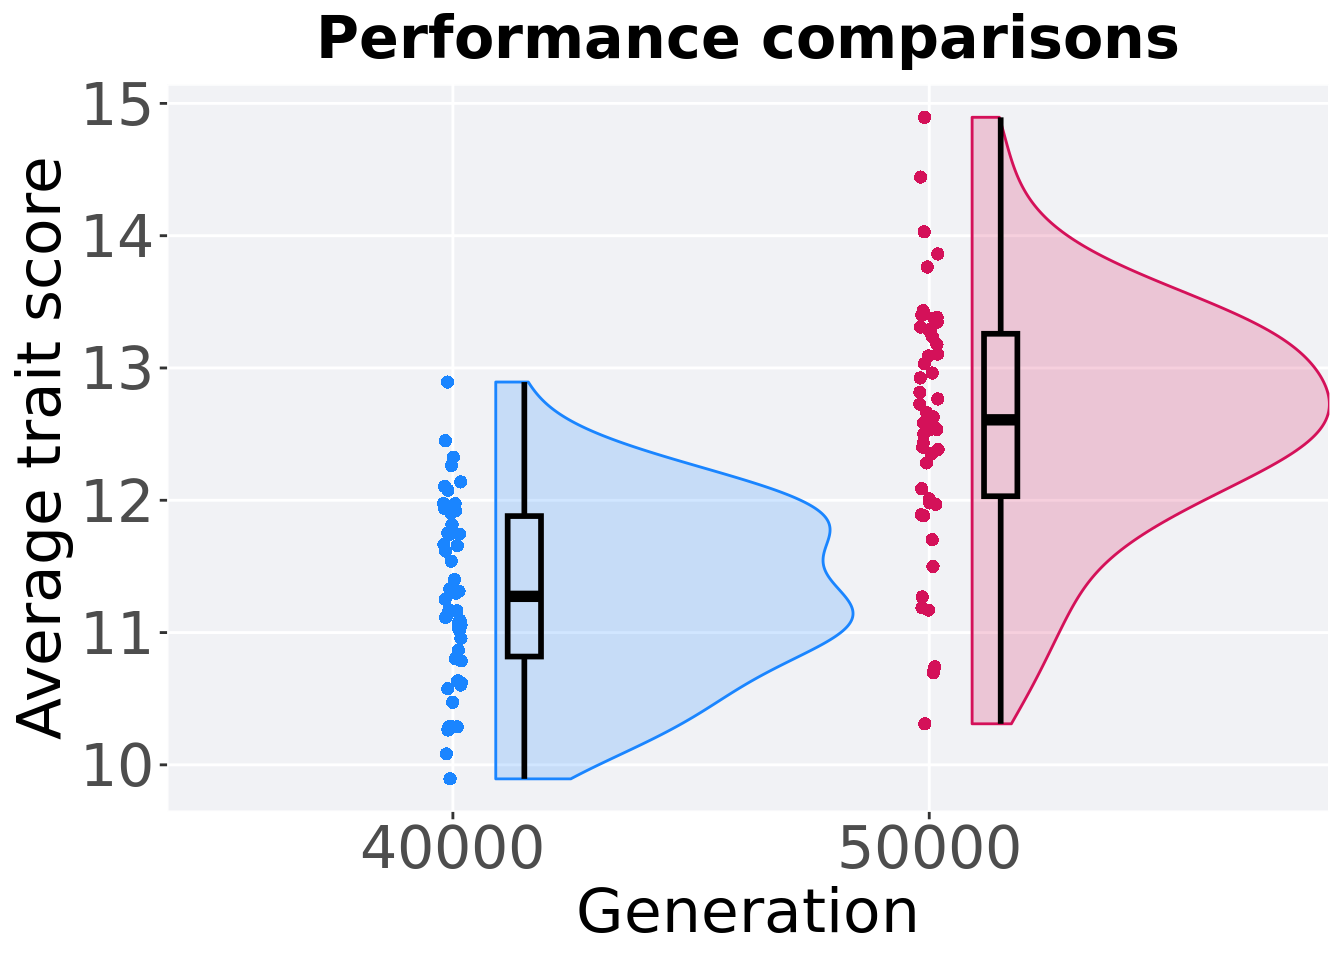
\includegraphics{mvc-diagnostics_files/figure-latex/exp-per-cmp-plt-ran-1.pdf}

Summary statistics for the best performance.

\begin{Shaded}
\begin{Highlighting}[]
\KeywordTok{filter}\NormalTok{(interval_df, acro }\OperatorTok{==}\StringTok{ 'ran'}\NormalTok{) }\OperatorTok
\StringTok{  }\KeywordTok{group_by}\NormalTok{(Generation) }\OperatorTok
\StringTok{  }\NormalTok{dplyr}\OperatorTok{::}\KeywordTok{summarise}\NormalTok{(}
    \DataTypeTok{count =} \KeywordTok{n}\NormalTok{(),}
    \DataTypeTok{na_cnt =} \KeywordTok{sum}\NormalTok{(}\KeywordTok{is.na}\NormalTok{(pop_fit_max)),}
    \DataTypeTok{min =} \KeywordTok{min}\NormalTok{(pop_fit_max }\OperatorTok{/}\StringTok{ }\NormalTok{DIMENSIONALITY, }\DataTypeTok{na.rm =} \OtherTok{TRUE}\NormalTok{),}
    \DataTypeTok{median =} \KeywordTok{median}\NormalTok{(pop_fit_max }\OperatorTok{/}\StringTok{ }\NormalTok{DIMENSIONALITY, }\DataTypeTok{na.rm =} \OtherTok{TRUE}\NormalTok{),}
    \DataTypeTok{mean =} \KeywordTok{mean}\NormalTok{(pop_fit_max }\OperatorTok{/}\StringTok{ }\NormalTok{DIMENSIONALITY, }\DataTypeTok{na.rm =} \OtherTok{TRUE}\NormalTok{),}
    \DataTypeTok{max =} \KeywordTok{max}\NormalTok{(pop_fit_max }\OperatorTok{/}\StringTok{ }\NormalTok{DIMENSIONALITY, }\DataTypeTok{na.rm =} \OtherTok{TRUE}\NormalTok{),}
    \DataTypeTok{IQR =} \KeywordTok{IQR}\NormalTok{(pop_fit_max }\OperatorTok{/}\StringTok{ }\NormalTok{DIMENSIONALITY, }\DataTypeTok{na.rm =} \OtherTok{TRUE}\NormalTok{)}
\NormalTok{  )}
\end{Highlighting}
\end{Shaded}

\begin{verbatim}
## # A tibble: 2 x 8
##   Generation count na_cnt   min median  mean   max   IQR
##   <fct>      <int>  <int> <dbl>  <dbl> <dbl> <dbl> <dbl>
## 1 40000         50      0  9.89   11.3  11.3  12.9  1.06
## 2 50000         50      0 10.3    12.6  12.6  14.9  1.23
\end{verbatim}

Results for post-hoc Wilcoxon rank-sum test.

\begin{Shaded}
\begin{Highlighting}[]
\KeywordTok{wilcox.test}\NormalTok{(}\DataTypeTok{x =} \KeywordTok{filter}\NormalTok{(interval_df, acro }\OperatorTok{==}\StringTok{ 'ran'} \OperatorTok{&}\StringTok{ }\NormalTok{Generation }\OperatorTok{==}\StringTok{ }\DecValTok{50000}\NormalTok{)}\OperatorTok{$}\NormalTok{pop_fit_max,}
            \DataTypeTok{y =} \KeywordTok{filter}\NormalTok{(interval_df, acro }\OperatorTok{==}\StringTok{ 'ran'} \OperatorTok{&}\StringTok{ }\NormalTok{Generation }\OperatorTok{==}\StringTok{ }\DecValTok{40000}\NormalTok{)}\OperatorTok{$}\NormalTok{pop_fit_max,}
            \DataTypeTok{alternative =} \StringTok{'g'}\NormalTok{)}
\end{Highlighting}
\end{Shaded}

\begin{verbatim}
## 
##  Wilcoxon rank sum test with continuity correction
## 
## data:  filter(interval_df, acro == "ran" & Generation == 50000)$pop_fit_max and filter(interval_df, acro == "ran" & Generation == 40000)$pop_fit_max
## W = 2185, p-value = 5.885e-11
## alternative hypothesis: true location shift is greater than 0
\end{verbatim}

\hypertarget{ordered-exploitation-results}{%
\chapter{Ordered exploitation results}\label{ordered-exploitation-results}}

Here we present the results for \textbf{best performances} found by each selection scheme on the ordered exploitation diagnostic with valley crossing integrated.
50 replicates are conducted for each scheme explored.

\hypertarget{analysis-dependencies-1}{%
\section{Analysis dependencies}\label{analysis-dependencies-1}}

\begin{Shaded}
\begin{Highlighting}[]
\KeywordTok{library}\NormalTok{(ggplot2)}
\KeywordTok{library}\NormalTok{(cowplot)}
\KeywordTok{library}\NormalTok{(dplyr)}
\KeywordTok{library}\NormalTok{(PupillometryR)}
\end{Highlighting}
\end{Shaded}

\hypertarget{data-setup-1}{%
\section{Data setup}\label{data-setup-1}}

\begin{Shaded}
\begin{Highlighting}[]
\NormalTok{DIR =}\StringTok{ }\KeywordTok{paste}\NormalTok{(DATA_DIR,}\StringTok{'ORDERED_EXPLOITATION/'}\NormalTok{, }\DataTypeTok{sep =} \StringTok{""}\NormalTok{, }\DataTypeTok{collapse =} \OtherTok{NULL}\NormalTok{)}
\NormalTok{over_time_df <-}\StringTok{ }\KeywordTok{read.csv}\NormalTok{(}\KeywordTok{paste}\NormalTok{(DIR,}\StringTok{'over-time.csv'}\NormalTok{, }\DataTypeTok{sep =} \StringTok{""}\NormalTok{, }\DataTypeTok{collapse =} \OtherTok{NULL}\NormalTok{), }\DataTypeTok{header =} \OtherTok{TRUE}\NormalTok{, }\DataTypeTok{stringsAsFactors =} \OtherTok{FALSE}\NormalTok{)}
\NormalTok{over_time_df}\OperatorTok{$}\NormalTok{scheme <-}\StringTok{ }\KeywordTok{factor}\NormalTok{(over_time_df}\OperatorTok{$}\NormalTok{scheme, }\DataTypeTok{levels =}\NormalTok{ NAMES)}

\NormalTok{best_df <-}\StringTok{ }\KeywordTok{read.csv}\NormalTok{(}\KeywordTok{paste}\NormalTok{(DIR,}\StringTok{'best.csv'}\NormalTok{, }\DataTypeTok{sep =} \StringTok{""}\NormalTok{, }\DataTypeTok{collapse =} \OtherTok{NULL}\NormalTok{), }\DataTypeTok{header =} \OtherTok{TRUE}\NormalTok{, }\DataTypeTok{stringsAsFactors =} \OtherTok{FALSE}\NormalTok{)}
\NormalTok{best_df}\OperatorTok{$}\NormalTok{acro <-}\StringTok{ }\KeywordTok{factor}\NormalTok{(best_df}\OperatorTok{$}\NormalTok{acro, }\DataTypeTok{levels =}\NormalTok{ ACRO)}
\end{Highlighting}
\end{Shaded}

\hypertarget{performance-over-time-1}{%
\section{Performance over time}\label{performance-over-time-1}}

Best performance in a population over time.
Data points on the graph is the average performance across 50 replicates every 2000 generations.
Shading comes from the best and worse performance across 50 replicates.

\begin{Shaded}
\begin{Highlighting}[]
\NormalTok{lines =}\StringTok{ }\NormalTok{over_time_df }\OperatorTok
\StringTok{  }\KeywordTok{group_by}\NormalTok{(scheme, gen) }\OperatorTok
\StringTok{  }\NormalTok{dplyr}\OperatorTok{::}\KeywordTok{summarise}\NormalTok{(}
    \DataTypeTok{min =} \KeywordTok{min}\NormalTok{(pop_fit_max) }\OperatorTok{/}\StringTok{ }\NormalTok{DIMENSIONALITY,}
    \DataTypeTok{mean =} \KeywordTok{mean}\NormalTok{(pop_fit_max) }\OperatorTok{/}\StringTok{ }\NormalTok{DIMENSIONALITY,}
    \DataTypeTok{max =} \KeywordTok{max}\NormalTok{(pop_fit_max) }\OperatorTok{/}\StringTok{ }\NormalTok{DIMENSIONALITY}
\NormalTok{  )}
\end{Highlighting}
\end{Shaded}

\begin{verbatim}
## `summarise()` has grouped output by 'scheme'. You can override using the
## `.groups` argument.
\end{verbatim}

\begin{Shaded}
\begin{Highlighting}[]
\NormalTok{over_time_plot =}\StringTok{ }\KeywordTok{ggplot}\NormalTok{(lines, }\KeywordTok{aes}\NormalTok{(}\DataTypeTok{x=}\NormalTok{gen, }\DataTypeTok{y=}\NormalTok{mean, }\DataTypeTok{group =}\NormalTok{ scheme, }\DataTypeTok{fill =}\NormalTok{ scheme, }\DataTypeTok{color =}\NormalTok{ scheme, }\DataTypeTok{shape =}\NormalTok{ scheme)) }\OperatorTok{+}
\StringTok{  }\KeywordTok{geom_ribbon}\NormalTok{(}\KeywordTok{aes}\NormalTok{(}\DataTypeTok{ymin =}\NormalTok{ min, }\DataTypeTok{ymax =}\NormalTok{ max), }\DataTypeTok{alpha =} \FloatTok{0.1}\NormalTok{) }\OperatorTok{+}
\StringTok{  }\KeywordTok{geom_line}\NormalTok{(}\DataTypeTok{size =} \FloatTok{0.5}\NormalTok{) }\OperatorTok{+}
\StringTok{  }\KeywordTok{geom_point}\NormalTok{(}\DataTypeTok{data =} \KeywordTok{filter}\NormalTok{(lines, gen }\OperatorTok\StringTok{ }\DecValTok{2000} \OperatorTok{==}\StringTok{ }\DecValTok{0} \OperatorTok{&}\StringTok{ }\NormalTok{gen }\OperatorTok{!=}\StringTok{ }\DecValTok{0}\NormalTok{), }\DataTypeTok{size =} \FloatTok{1.5}\NormalTok{, }\DataTypeTok{stroke =} \FloatTok{2.0}\NormalTok{, }\DataTypeTok{alpha =} \FloatTok{1.0}\NormalTok{) }\OperatorTok{+}
\StringTok{  }\KeywordTok{scale_y_continuous}\NormalTok{(}
    \DataTypeTok{name=}\StringTok{"Average trait score"}\NormalTok{,}
    \DataTypeTok{limits=}\KeywordTok{c}\NormalTok{(}\DecValTok{0}\NormalTok{, }\DecValTok{15}\NormalTok{),}
\NormalTok{  ) }\OperatorTok{+}
\StringTok{  }\KeywordTok{scale_x_continuous}\NormalTok{(}
    \DataTypeTok{name=}\StringTok{"Generations"}\NormalTok{,}
    \DataTypeTok{limits=}\KeywordTok{c}\NormalTok{(}\DecValTok{0}\NormalTok{, }\DecValTok{50000}\NormalTok{),}
    \DataTypeTok{breaks=}\KeywordTok{c}\NormalTok{(}\DecValTok{0}\NormalTok{, }\DecValTok{10000}\NormalTok{, }\DecValTok{20000}\NormalTok{, }\DecValTok{30000}\NormalTok{, }\DecValTok{40000}\NormalTok{, }\DecValTok{50000}\NormalTok{),}
    \DataTypeTok{labels=}\KeywordTok{c}\NormalTok{(}\StringTok{"0e+4"}\NormalTok{, }\StringTok{"1e+4"}\NormalTok{, }\StringTok{"2e+4"}\NormalTok{, }\StringTok{"3e+4"}\NormalTok{, }\StringTok{"4e+4"}\NormalTok{, }\StringTok{"5e+4"}\NormalTok{)}

\NormalTok{  ) }\OperatorTok{+}
\StringTok{  }\KeywordTok{scale_shape_manual}\NormalTok{(}\DataTypeTok{values=}\NormalTok{SHAPE)}\OperatorTok{+}
\StringTok{  }\KeywordTok{scale_colour_manual}\NormalTok{(}\DataTypeTok{values =}\NormalTok{ cb_palette) }\OperatorTok{+}
\StringTok{  }\KeywordTok{scale_fill_manual}\NormalTok{(}\DataTypeTok{values =}\NormalTok{ cb_palette) }\OperatorTok{+}
\StringTok{  }\KeywordTok{ggtitle}\NormalTok{(}\StringTok{'Performance over time'}\NormalTok{)}\OperatorTok{+}
\StringTok{  }\NormalTok{p_theme }\OperatorTok{+}\StringTok{ }\KeywordTok{theme}\NormalTok{(}\DataTypeTok{legend.title=}\KeywordTok{element_blank}\NormalTok{(),}\DataTypeTok{legend.text=}\KeywordTok{element_text}\NormalTok{(}\DataTypeTok{size=}\DecValTok{12}\NormalTok{)) }\OperatorTok{+}
\StringTok{  }\KeywordTok{guides}\NormalTok{(}
    \DataTypeTok{shape=}\KeywordTok{guide_legend}\NormalTok{(}\DataTypeTok{ncol=}\DecValTok{2}\NormalTok{, }\DataTypeTok{title.position =} \StringTok{"bottom"}\NormalTok{),}
    \DataTypeTok{color=}\KeywordTok{guide_legend}\NormalTok{(}\DataTypeTok{ncol=}\DecValTok{2}\NormalTok{, }\DataTypeTok{title.position =} \StringTok{"bottom"}\NormalTok{),}
    \DataTypeTok{fill=}\KeywordTok{guide_legend}\NormalTok{(}\DataTypeTok{ncol=}\DecValTok{2}\NormalTok{, }\DataTypeTok{title.position =} \StringTok{"bottom"}\NormalTok{)}
\NormalTok{  )}

\NormalTok{over_time_plot}
\end{Highlighting}
\end{Shaded}

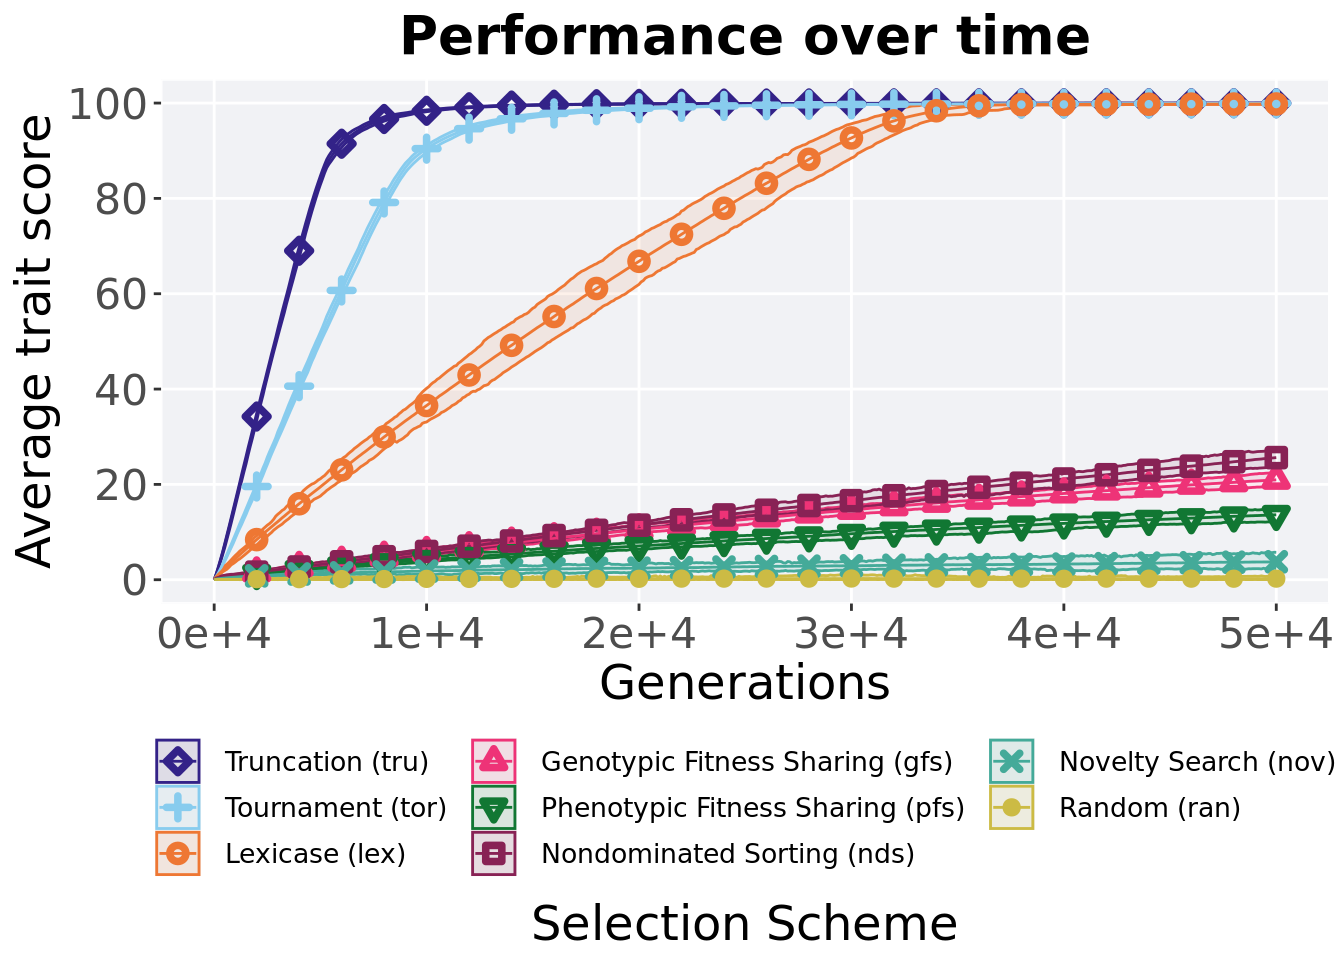
\includegraphics{mvc-diagnostics_files/figure-latex/ord-per-ot-1.pdf}

\hypertarget{best-performance-throughout-1}{%
\section{Best performance throughout}\label{best-performance-throughout-1}}

Best performance reached throughout 50,000 generations in a population.

\begin{Shaded}
\begin{Highlighting}[]
\NormalTok{plot =}\StringTok{ }\KeywordTok{filter}\NormalTok{(best_df, var }\OperatorTok{==}\StringTok{ 'pop_fit_max'}\NormalTok{) }\OperatorTok
\StringTok{  }\KeywordTok{ggplot}\NormalTok{(., }\KeywordTok{aes}\NormalTok{(}\DataTypeTok{x =}\NormalTok{ acro, }\DataTypeTok{y =}\NormalTok{ val }\OperatorTok{/}\StringTok{ }\NormalTok{DIMENSIONALITY, }\DataTypeTok{color =}\NormalTok{ acro, }\DataTypeTok{fill =}\NormalTok{ acro, }\DataTypeTok{shape =}\NormalTok{ acro)) }\OperatorTok{+}
\StringTok{  }\KeywordTok{geom_flat_violin}\NormalTok{(}\DataTypeTok{position =} \KeywordTok{position_nudge}\NormalTok{(}\DataTypeTok{x =} \FloatTok{.09}\NormalTok{, }\DataTypeTok{y =} \DecValTok{0}\NormalTok{), }\DataTypeTok{scale =} \StringTok{'width'}\NormalTok{, }\DataTypeTok{alpha =} \FloatTok{0.2}\NormalTok{, }\DataTypeTok{width =} \FloatTok{1.5}\NormalTok{) }\OperatorTok{+}
\StringTok{  }\KeywordTok{geom_boxplot}\NormalTok{(}\DataTypeTok{color =} \StringTok{'black'}\NormalTok{, }\DataTypeTok{width =} \FloatTok{.07}\NormalTok{, }\DataTypeTok{outlier.shape =} \OtherTok{NA}\NormalTok{, }\DataTypeTok{alpha =} \FloatTok{0.0}\NormalTok{, }\DataTypeTok{size =} \FloatTok{1.0}\NormalTok{, }\DataTypeTok{position =} \KeywordTok{position_nudge}\NormalTok{(}\DataTypeTok{x =} \FloatTok{.15}\NormalTok{, }\DataTypeTok{y =} \DecValTok{0}\NormalTok{)) }\OperatorTok{+}
\StringTok{  }\KeywordTok{geom_point}\NormalTok{(}\DataTypeTok{position =} \KeywordTok{position_jitter}\NormalTok{(}\DataTypeTok{width =} \FloatTok{.02}\NormalTok{), }\DataTypeTok{size =} \FloatTok{2.0}\NormalTok{, }\DataTypeTok{alpha =} \FloatTok{1.0}\NormalTok{) }\OperatorTok{+}
\StringTok{  }\KeywordTok{scale_y_continuous}\NormalTok{(}
    \DataTypeTok{name=}\StringTok{"Average trait score"}
\NormalTok{  ) }\OperatorTok{+}
\StringTok{  }\KeywordTok{scale_x_discrete}\NormalTok{(}
    \DataTypeTok{name=}\StringTok{"Scheme"}
\NormalTok{  )}\OperatorTok{+}
\StringTok{  }\KeywordTok{scale_shape_manual}\NormalTok{(}\DataTypeTok{values=}\NormalTok{SHAPE)}\OperatorTok{+}
\StringTok{  }\KeywordTok{scale_colour_manual}\NormalTok{(}\DataTypeTok{values =}\NormalTok{ cb_palette, ) }\OperatorTok{+}
\StringTok{  }\KeywordTok{scale_fill_manual}\NormalTok{(}\DataTypeTok{values =}\NormalTok{ cb_palette) }\OperatorTok{+}
\StringTok{  }\KeywordTok{ggtitle}\NormalTok{(}\StringTok{'Best performance throughout'}\NormalTok{)}\OperatorTok{+}
\StringTok{  }\NormalTok{p_theme }\OperatorTok{+}\StringTok{ }\KeywordTok{theme}\NormalTok{(}\DataTypeTok{legend.title=}\KeywordTok{element_blank}\NormalTok{())}

\KeywordTok{plot_grid}\NormalTok{(}
\NormalTok{  plot }\OperatorTok{+}
\StringTok{    }\KeywordTok{theme}\NormalTok{(}\DataTypeTok{legend.position=}\StringTok{"none"}\NormalTok{),}
\NormalTok{  legend,}
  \DataTypeTok{nrow=}\DecValTok{2}\NormalTok{,}
  \DataTypeTok{rel_heights =} \KeywordTok{c}\NormalTok{(}\DecValTok{3}\NormalTok{,}\DecValTok{1}\NormalTok{)}
\NormalTok{)}
\end{Highlighting}
\end{Shaded}

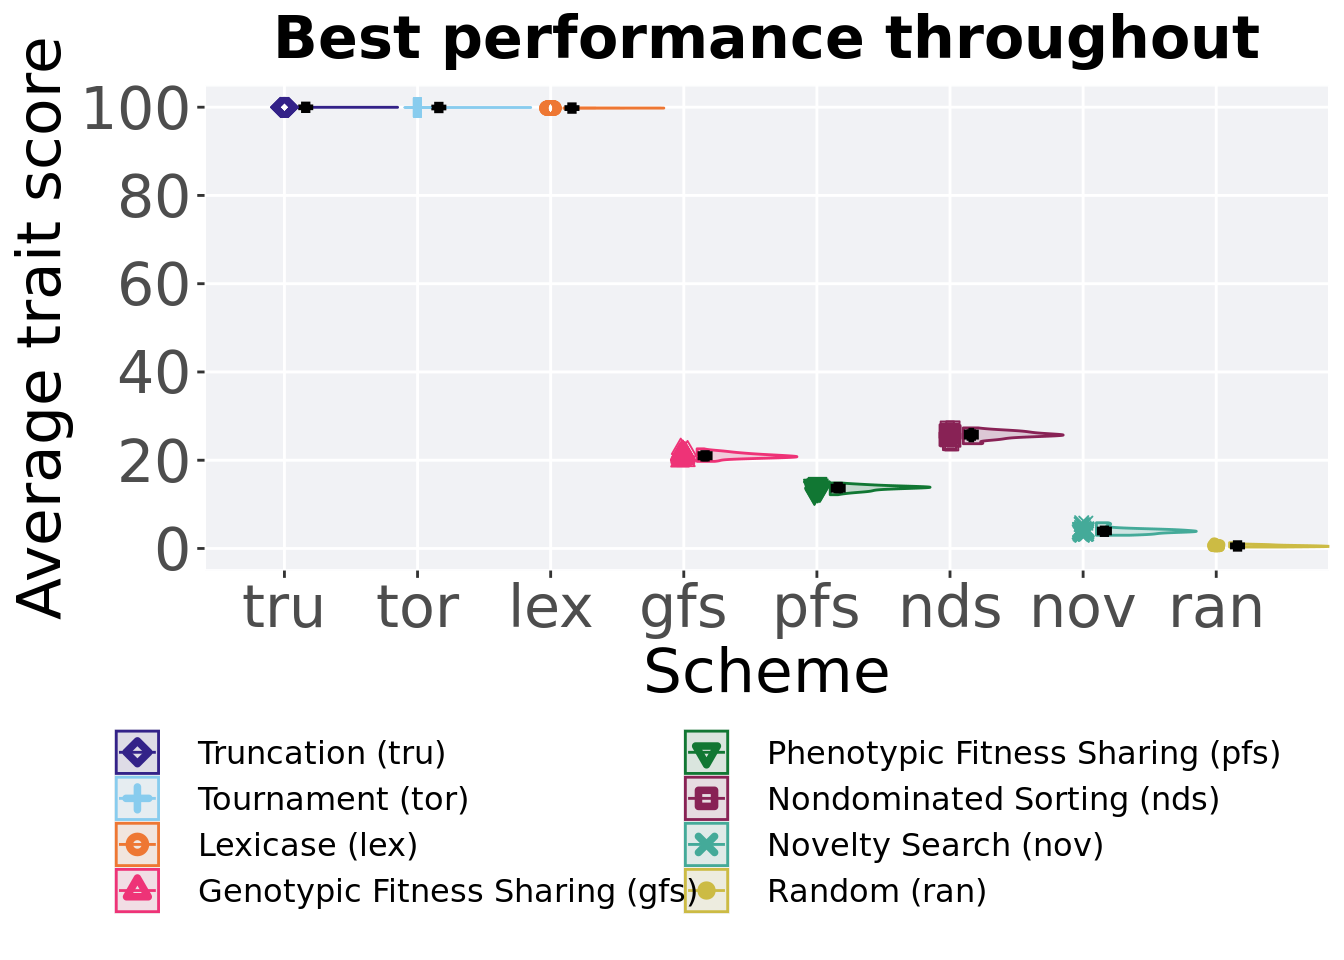
\includegraphics{mvc-diagnostics_files/figure-latex/ord-per-bst-1.pdf}

\hypertarget{stats-1}{%
\subsection{Stats}\label{stats-1}}

Summary statistics for the best performance.

\begin{Shaded}
\begin{Highlighting}[]
\NormalTok{performance =}\StringTok{ }\KeywordTok{filter}\NormalTok{(best_df, var }\OperatorTok{==}\StringTok{ 'pop_fit_max'}\NormalTok{)}
\NormalTok{performance}\OperatorTok{$}\NormalTok{acro =}\StringTok{ }\KeywordTok{factor}\NormalTok{(performance}\OperatorTok{$}\NormalTok{acro, }\DataTypeTok{levels =} \KeywordTok{c}\NormalTok{(}\StringTok{'gfs'}\NormalTok{,}\StringTok{'pfs'}\NormalTok{,}\StringTok{'tru'}\NormalTok{,}\StringTok{'tor'}\NormalTok{,}\StringTok{'lex'}\NormalTok{,}\StringTok{'nov'}\NormalTok{,}\StringTok{'nds'}\NormalTok{,}\StringTok{'ran'}\NormalTok{))}
\NormalTok{performance }\OperatorTok
\StringTok{  }\KeywordTok{group_by}\NormalTok{(acro) }\OperatorTok
\StringTok{  }\NormalTok{dplyr}\OperatorTok{::}\KeywordTok{summarise}\NormalTok{(}
    \DataTypeTok{count =} \KeywordTok{n}\NormalTok{(),}
    \DataTypeTok{na_cnt =} \KeywordTok{sum}\NormalTok{(}\KeywordTok{is.na}\NormalTok{(val)),}
    \DataTypeTok{min =} \KeywordTok{min}\NormalTok{(val }\OperatorTok{/}\StringTok{ }\NormalTok{DIMENSIONALITY, }\DataTypeTok{na.rm =} \OtherTok{TRUE}\NormalTok{),}
    \DataTypeTok{median =} \KeywordTok{median}\NormalTok{(val }\OperatorTok{/}\StringTok{ }\NormalTok{DIMENSIONALITY, }\DataTypeTok{na.rm =} \OtherTok{TRUE}\NormalTok{),}
    \DataTypeTok{mean =} \KeywordTok{mean}\NormalTok{(val }\OperatorTok{/}\StringTok{ }\NormalTok{DIMENSIONALITY, }\DataTypeTok{na.rm =} \OtherTok{TRUE}\NormalTok{),}
    \DataTypeTok{max =} \KeywordTok{max}\NormalTok{(val }\OperatorTok{/}\StringTok{ }\NormalTok{DIMENSIONALITY, }\DataTypeTok{na.rm =} \OtherTok{TRUE}\NormalTok{),}
    \DataTypeTok{IQR =} \KeywordTok{IQR}\NormalTok{(val }\OperatorTok{/}\StringTok{ }\NormalTok{DIMENSIONALITY, }\DataTypeTok{na.rm =} \OtherTok{TRUE}\NormalTok{)}
\NormalTok{  )}
\end{Highlighting}
\end{Shaded}

\begin{verbatim}
## # A tibble: 8 x 8
##   acro  count na_cnt    min median   mean   max   IQR
##   <fct> <int>  <int>  <dbl>  <dbl>  <dbl> <dbl> <dbl>
## 1 gfs      50      0 10.2   11.7   11.7   12.8  0.876
## 2 pfs      50      0 10.2   11.1   11.2   12.2  0.840
## 3 tru      50      0  6.07   8.35   8.23   8.72 0.166
## 4 tor      50      0  5.60   8.26   7.79   8.61 1.07 
## 5 lex      50      0  5.44   6.83   6.72   7.78 0.949
## 6 nov      50      0  2.84   3.70   3.74   4.89 0.555
## 7 nds      50      0  1.74   1.84   1.85   2.16 0.114
## 8 ran      50      0  0.192  0.552  0.570  1.50 0.269
\end{verbatim}

Kruskal--Wallis test illustrates evidence of statistical differences.

\begin{Shaded}
\begin{Highlighting}[]
\KeywordTok{kruskal.test}\NormalTok{(val }\OperatorTok{~}\StringTok{ }\NormalTok{acro, }\DataTypeTok{data =}\NormalTok{ performance)}
\end{Highlighting}
\end{Shaded}

\begin{verbatim}
## 
##  Kruskal-Wallis rank sum test
## 
## data:  val by acro
## Kruskal-Wallis chi-squared = 380.24, df = 7, p-value < 2.2e-16
\end{verbatim}

Results for post-hoc Wilcoxon rank-sum test with a Bonferroni correction.

\begin{Shaded}
\begin{Highlighting}[]
\KeywordTok{pairwise.wilcox.test}\NormalTok{(}\DataTypeTok{x =}\NormalTok{ performance}\OperatorTok{$}\NormalTok{val, }\DataTypeTok{g =}\NormalTok{ performance}\OperatorTok{$}\NormalTok{acro, }\DataTypeTok{p.adjust.method =} \StringTok{"bonferroni"}\NormalTok{,}
                     \DataTypeTok{paired =} \OtherTok{FALSE}\NormalTok{, }\DataTypeTok{conf.int =} \OtherTok{FALSE}\NormalTok{, }\DataTypeTok{alternative =} \StringTok{'l'}\NormalTok{)}
\end{Highlighting}
\end{Shaded}

\begin{verbatim}
## 
##  Pairwise comparisons using Wilcoxon rank sum test with continuity correction 
## 
## data:  performance$val and performance$acro 
## 
##     gfs     pfs     tru     tor     lex     nov     nds    
## pfs 0.00041 -       -       -       -       -       -      
## tru < 2e-16 < 2e-16 -       -       -       -       -      
## tor < 2e-16 < 2e-16 0.09539 -       -       -       -      
## lex < 2e-16 < 2e-16 2.1e-14 2.0e-07 -       -       -      
## nov < 2e-16 < 2e-16 < 2e-16 < 2e-16 < 2e-16 -       -      
## nds < 2e-16 < 2e-16 < 2e-16 < 2e-16 < 2e-16 < 2e-16 -      
## ran < 2e-16 < 2e-16 < 2e-16 < 2e-16 < 2e-16 < 2e-16 < 2e-16
## 
## P value adjustment method: bonferroni
\end{verbatim}

\hypertarget{performance-interval-comparison-1}{%
\section{Performance interval comparison}\label{performance-interval-comparison-1}}

Here we compare the best performance found in the population at generation 40,000 \& 50,000 for all selection schemes.

\begin{Shaded}
\begin{Highlighting}[]
\NormalTok{interval_df =}\StringTok{ }\KeywordTok{filter}\NormalTok{(}\KeywordTok{filter}\NormalTok{(over_time_df, (gen }\OperatorTok{==}\StringTok{ }\DecValTok{50000} \OperatorTok{|}\StringTok{ }\NormalTok{gen }\OperatorTok{==}\StringTok{ }\DecValTok{40000}\NormalTok{)))}
\NormalTok{interval_df}\OperatorTok{$}\NormalTok{Generation <-}\StringTok{ }\KeywordTok{factor}\NormalTok{(interval_df}\OperatorTok{$}\NormalTok{gen, }\DataTypeTok{levels =} \KeywordTok{c}\NormalTok{(}\DecValTok{40000}\NormalTok{,}\DecValTok{50000}\NormalTok{))}
\NormalTok{interval_df}\OperatorTok{$}\NormalTok{acro <-}\StringTok{ }\KeywordTok{factor}\NormalTok{(interval_df}\OperatorTok{$}\NormalTok{acro, }\DataTypeTok{levels =}\NormalTok{ ACRO)}

\KeywordTok{ggplot}\NormalTok{(interval_df, }\KeywordTok{aes}\NormalTok{(}\DataTypeTok{x=}\NormalTok{acro, }\DataTypeTok{y=}\NormalTok{pop_fit_max}\OperatorTok{/}\NormalTok{DIMENSIONALITY,}\DataTypeTok{fill=}\NormalTok{Generation,}\DataTypeTok{color=}\NormalTok{Generation,}\DataTypeTok{shape=}\NormalTok{Generation)) }\OperatorTok{+}
\StringTok{  }\KeywordTok{geom_boxplot}\NormalTok{(}\DataTypeTok{width =} \FloatTok{.3}\NormalTok{, }\DataTypeTok{outlier.shape =} \OtherTok{NA}\NormalTok{, }\DataTypeTok{alpha =} \FloatTok{0.0}\NormalTok{) }\OperatorTok{+}
\StringTok{  }\KeywordTok{geom_point}\NormalTok{(}\DataTypeTok{size =} \FloatTok{1.0}\NormalTok{, }\DataTypeTok{alpha =} \FloatTok{1.0}\NormalTok{, }\DataTypeTok{position=}\KeywordTok{position_dodge}\NormalTok{(}\DataTypeTok{width=}\FloatTok{1.0}\NormalTok{)) }\OperatorTok{+}
\StringTok{    }\KeywordTok{scale_y_continuous}\NormalTok{(}
      \DataTypeTok{name=}\StringTok{"Average trait score"}
\NormalTok{    ) }\OperatorTok{+}
\StringTok{    }\KeywordTok{scale_x_discrete}\NormalTok{(}
      \DataTypeTok{name=}\StringTok{"Scheme"}
\NormalTok{    ) }\OperatorTok{+}
\StringTok{  }\KeywordTok{scale_shape_manual}\NormalTok{(}\DataTypeTok{values=}\NormalTok{SHAPE)}\OperatorTok{+}
\StringTok{  }\KeywordTok{scale_colour_manual}\NormalTok{(}\DataTypeTok{values =}\NormalTok{ mvc_col, ) }\OperatorTok{+}
\StringTok{  }\KeywordTok{scale_fill_manual}\NormalTok{(}\DataTypeTok{values =}\NormalTok{ mvc_col) }\OperatorTok{+}
\StringTok{  }\KeywordTok{ggtitle}\NormalTok{(}\StringTok{'Performance comparisons'}\NormalTok{)}\OperatorTok{+}
\StringTok{  }\NormalTok{p_theme}
\end{Highlighting}
\end{Shaded}

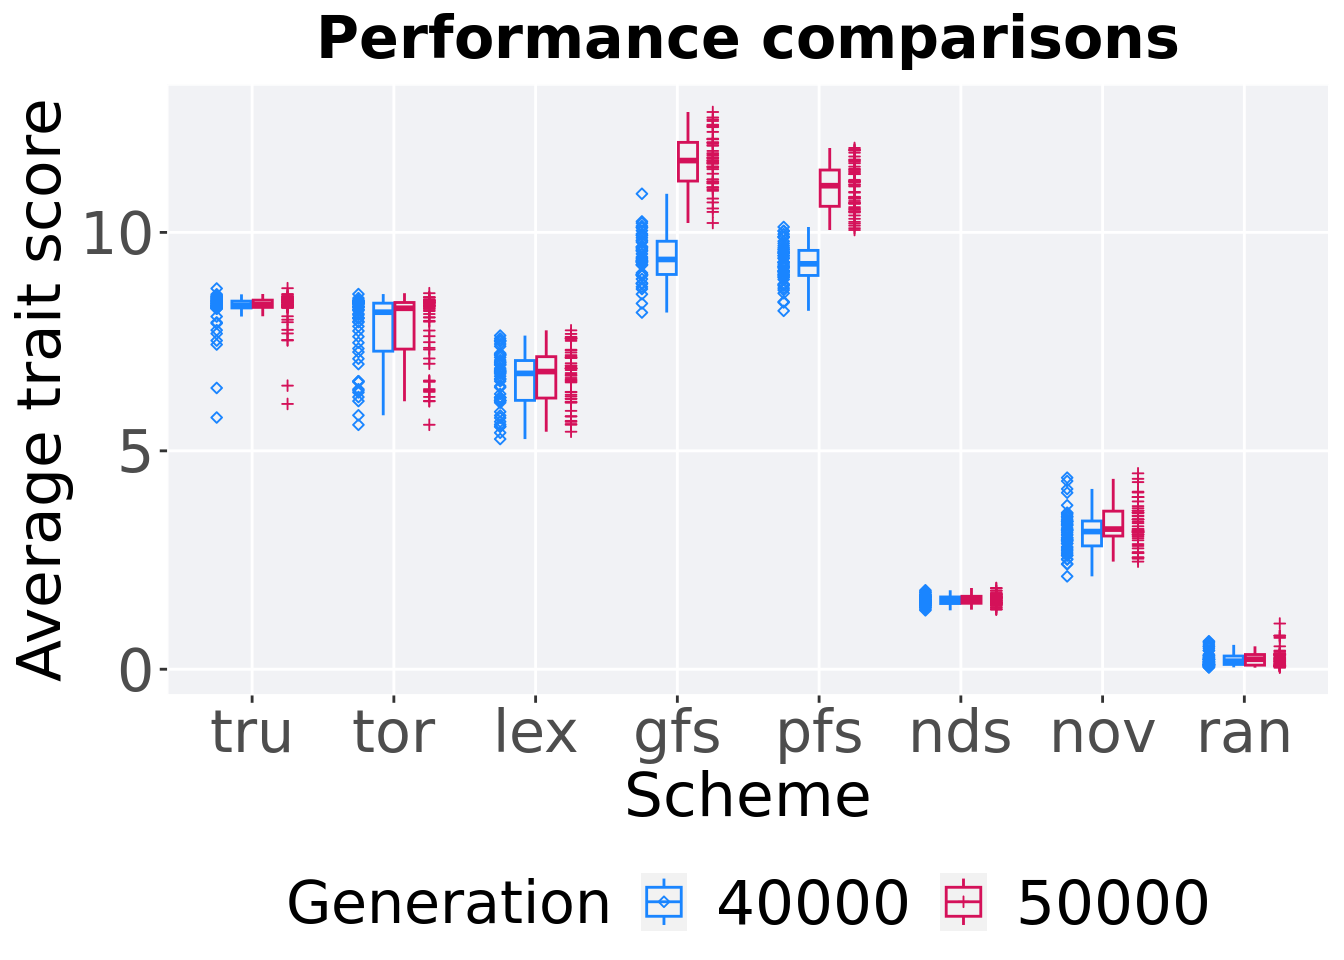
\includegraphics{mvc-diagnostics_files/figure-latex/ord-per-cmp-1.pdf}

\hypertarget{stats-by-interval-comparisons-1}{%
\subsection{Stats by interval comparisons}\label{stats-by-interval-comparisons-1}}

Here we present statistical analysis between the performances found at different generation intervals.

\hypertarget{truncation-1}{%
\subsubsection{Truncation}\label{truncation-1}}

Plot for comparing performances at interval 40,000 \& 50,000.

\begin{Shaded}
\begin{Highlighting}[]
\KeywordTok{filter}\NormalTok{(interval_df, acro }\OperatorTok{==}\StringTok{ 'tru'}\NormalTok{) }\OperatorTok
\KeywordTok{ggplot}\NormalTok{(., }\KeywordTok{aes}\NormalTok{(}\DataTypeTok{x=}\NormalTok{Generation, }\DataTypeTok{y=}\NormalTok{pop_fit_max}\OperatorTok{/}\NormalTok{DIMENSIONALITY,}\DataTypeTok{fill=}\NormalTok{Generation,}\DataTypeTok{color=}\NormalTok{Generation,}\DataTypeTok{shape=}\NormalTok{Generation)) }\OperatorTok{+}
\StringTok{  }\KeywordTok{geom_flat_violin}\NormalTok{(}\DataTypeTok{position =} \KeywordTok{position_nudge}\NormalTok{(}\DataTypeTok{x =} \FloatTok{.09}\NormalTok{, }\DataTypeTok{y =} \DecValTok{0}\NormalTok{), }\DataTypeTok{scale =} \StringTok{'width'}\NormalTok{, }\DataTypeTok{alpha =} \FloatTok{0.2}\NormalTok{, }\DataTypeTok{width =} \FloatTok{1.5}\NormalTok{) }\OperatorTok{+}
\StringTok{  }\KeywordTok{geom_boxplot}\NormalTok{(}\DataTypeTok{color =} \StringTok{'black'}\NormalTok{, }\DataTypeTok{width =} \FloatTok{.07}\NormalTok{, }\DataTypeTok{outlier.shape =} \OtherTok{NA}\NormalTok{, }\DataTypeTok{alpha =} \FloatTok{0.0}\NormalTok{, }\DataTypeTok{size =} \FloatTok{1.0}\NormalTok{, }\DataTypeTok{position =} \KeywordTok{position_nudge}\NormalTok{(}\DataTypeTok{x =} \FloatTok{.15}\NormalTok{, }\DataTypeTok{y =} \DecValTok{0}\NormalTok{)) }\OperatorTok{+}
\StringTok{  }\KeywordTok{geom_point}\NormalTok{(}\DataTypeTok{position =} \KeywordTok{position_jitter}\NormalTok{(}\DataTypeTok{width =} \FloatTok{.02}\NormalTok{), }\DataTypeTok{size =} \FloatTok{2.0}\NormalTok{, }\DataTypeTok{alpha =} \FloatTok{1.0}\NormalTok{) }\OperatorTok{+}
\StringTok{    }\KeywordTok{scale_y_continuous}\NormalTok{(}
      \DataTypeTok{name=}\StringTok{"Average trait score"}\NormalTok{,}
\NormalTok{    ) }\OperatorTok{+}
\StringTok{    }\KeywordTok{scale_x_discrete}\NormalTok{(}
      \DataTypeTok{name=}\StringTok{"Generation"}
\NormalTok{    ) }\OperatorTok{+}
\StringTok{  }\KeywordTok{scale_shape_manual}\NormalTok{(}\DataTypeTok{values=}\KeywordTok{c}\NormalTok{(}\DecValTok{16}\NormalTok{,}\DecValTok{16}\NormalTok{))}\OperatorTok{+}
\StringTok{  }\KeywordTok{scale_colour_manual}\NormalTok{(}\DataTypeTok{values =}\NormalTok{ mvc_col, ) }\OperatorTok{+}
\StringTok{  }\KeywordTok{scale_fill_manual}\NormalTok{(}\DataTypeTok{values =}\NormalTok{ mvc_col) }\OperatorTok{+}
\StringTok{  }\KeywordTok{ggtitle}\NormalTok{(}\StringTok{'Performance comparisons'}\NormalTok{)}\OperatorTok{+}
\StringTok{  }\NormalTok{p_theme }\OperatorTok{+}\StringTok{ }\KeywordTok{theme}\NormalTok{(}\DataTypeTok{legend.position=}\StringTok{"none"}\NormalTok{)}
\end{Highlighting}
\end{Shaded}

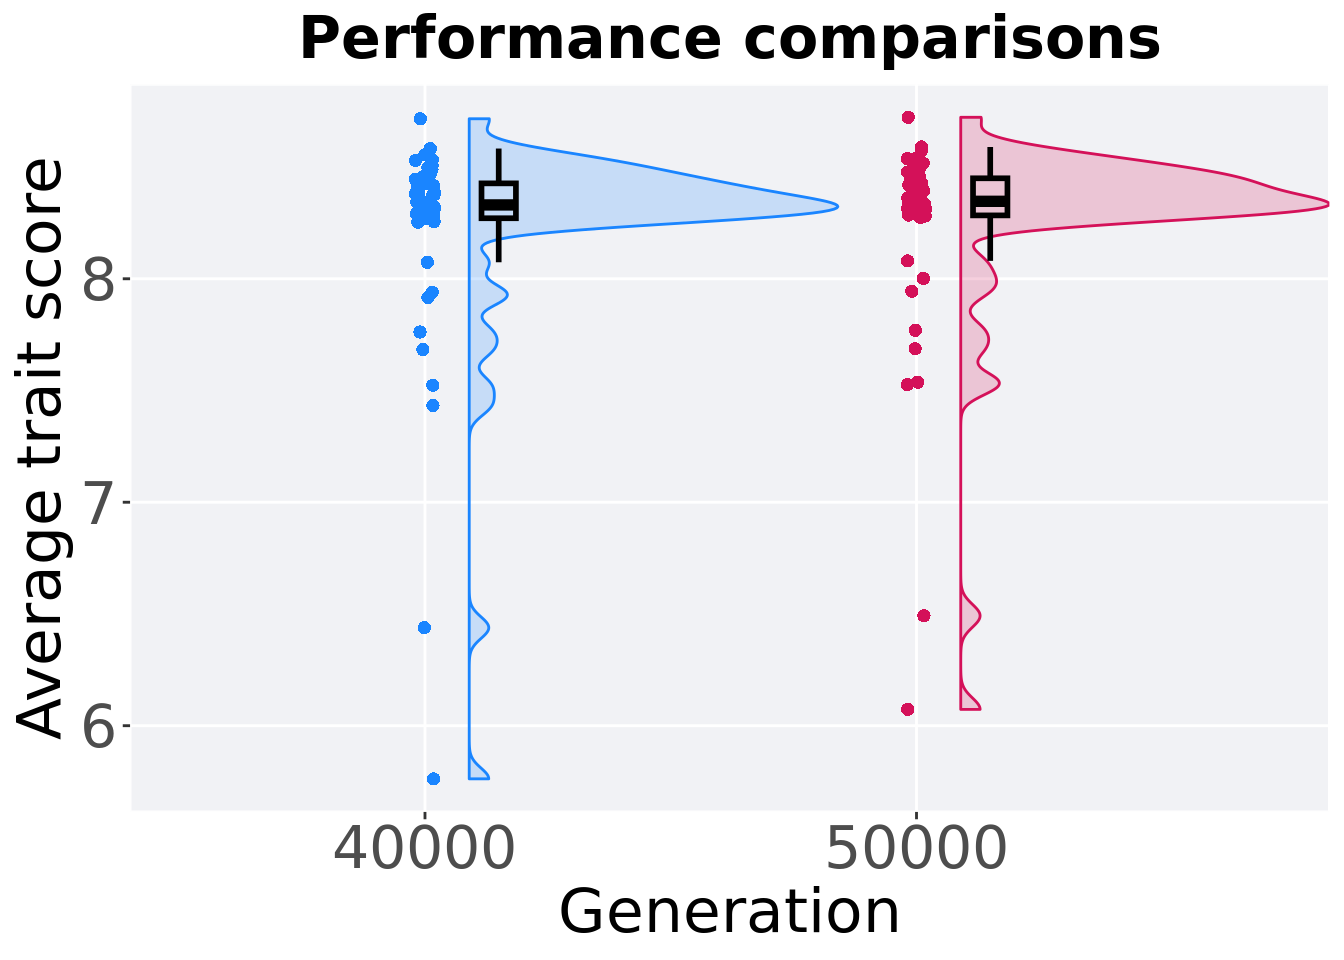
\includegraphics{mvc-diagnostics_files/figure-latex/ord-per-cmp-plt-tru-1.pdf}

Summary statistics for the best performance.

\begin{Shaded}
\begin{Highlighting}[]
\KeywordTok{filter}\NormalTok{(interval_df, acro }\OperatorTok{==}\StringTok{ 'tru'}\NormalTok{) }\OperatorTok
\StringTok{  }\KeywordTok{group_by}\NormalTok{(Generation) }\OperatorTok
\StringTok{  }\NormalTok{dplyr}\OperatorTok{::}\KeywordTok{summarise}\NormalTok{(}
    \DataTypeTok{count =} \KeywordTok{n}\NormalTok{(),}
    \DataTypeTok{na_cnt =} \KeywordTok{sum}\NormalTok{(}\KeywordTok{is.na}\NormalTok{(pop_fit_max)),}
    \DataTypeTok{min =} \KeywordTok{min}\NormalTok{(pop_fit_max }\OperatorTok{/}\StringTok{ }\NormalTok{DIMENSIONALITY, }\DataTypeTok{na.rm =} \OtherTok{TRUE}\NormalTok{),}
    \DataTypeTok{median =} \KeywordTok{median}\NormalTok{(pop_fit_max }\OperatorTok{/}\StringTok{ }\NormalTok{DIMENSIONALITY, }\DataTypeTok{na.rm =} \OtherTok{TRUE}\NormalTok{),}
    \DataTypeTok{mean =} \KeywordTok{mean}\NormalTok{(pop_fit_max }\OperatorTok{/}\StringTok{ }\NormalTok{DIMENSIONALITY, }\DataTypeTok{na.rm =} \OtherTok{TRUE}\NormalTok{),}
    \DataTypeTok{max =} \KeywordTok{max}\NormalTok{(pop_fit_max }\OperatorTok{/}\StringTok{ }\NormalTok{DIMENSIONALITY, }\DataTypeTok{na.rm =} \OtherTok{TRUE}\NormalTok{),}
    \DataTypeTok{IQR =} \KeywordTok{IQR}\NormalTok{(pop_fit_max }\OperatorTok{/}\StringTok{ }\NormalTok{DIMENSIONALITY, }\DataTypeTok{na.rm =} \OtherTok{TRUE}\NormalTok{)}
\NormalTok{  )}
\end{Highlighting}
\end{Shaded}

\begin{verbatim}
## # A tibble: 2 x 8
##   Generation count na_cnt   min median  mean   max   IQR
##   <fct>      <int>  <int> <dbl>  <dbl> <dbl> <dbl> <dbl>
## 1 40000         50      0  5.76   8.33  8.21  8.72 0.156
## 2 50000         50      0  6.07   8.35  8.23  8.72 0.166
\end{verbatim}

Results for post-hoc Wilcoxon rank-sum test.

\begin{Shaded}
\begin{Highlighting}[]
\KeywordTok{wilcox.test}\NormalTok{(}\DataTypeTok{x =} \KeywordTok{filter}\NormalTok{(interval_df, acro }\OperatorTok{==}\StringTok{ 'tru'} \OperatorTok{&}\StringTok{ }\NormalTok{Generation }\OperatorTok{==}\StringTok{ }\DecValTok{50000}\NormalTok{)}\OperatorTok{$}\NormalTok{pop_fit_max,}
            \DataTypeTok{y =} \KeywordTok{filter}\NormalTok{(interval_df, acro }\OperatorTok{==}\StringTok{ 'tru'} \OperatorTok{&}\StringTok{ }\NormalTok{Generation }\OperatorTok{==}\StringTok{ }\DecValTok{40000}\NormalTok{)}\OperatorTok{$}\NormalTok{pop_fit_max,}
            \DataTypeTok{alternative =} \StringTok{'t'}\NormalTok{)}
\end{Highlighting}
\end{Shaded}

\begin{verbatim}
## 
##  Wilcoxon rank sum test with continuity correction
## 
## data:  filter(interval_df, acro == "tru" & Generation == 50000)$pop_fit_max and filter(interval_df, acro == "tru" & Generation == 40000)$pop_fit_max
## W = 1351, p-value = 0.4884
## alternative hypothesis: true location shift is not equal to 0
\end{verbatim}

\hypertarget{tournament-1}{%
\subsubsection{Tournament}\label{tournament-1}}

Plot for comparing performances at interval 40,000 \& 50,000.

\begin{Shaded}
\begin{Highlighting}[]
\KeywordTok{filter}\NormalTok{(interval_df, acro }\OperatorTok{==}\StringTok{ 'tor'}\NormalTok{) }\OperatorTok
\KeywordTok{ggplot}\NormalTok{(., }\KeywordTok{aes}\NormalTok{(}\DataTypeTok{x=}\NormalTok{Generation, }\DataTypeTok{y=}\NormalTok{pop_fit_max}\OperatorTok{/}\NormalTok{DIMENSIONALITY,}\DataTypeTok{fill=}\NormalTok{Generation,}\DataTypeTok{color=}\NormalTok{Generation,}\DataTypeTok{shape=}\NormalTok{Generation)) }\OperatorTok{+}
\StringTok{  }\KeywordTok{geom_flat_violin}\NormalTok{(}\DataTypeTok{position =} \KeywordTok{position_nudge}\NormalTok{(}\DataTypeTok{x =} \FloatTok{.09}\NormalTok{, }\DataTypeTok{y =} \DecValTok{0}\NormalTok{), }\DataTypeTok{scale =} \StringTok{'width'}\NormalTok{, }\DataTypeTok{alpha =} \FloatTok{0.2}\NormalTok{, }\DataTypeTok{width =} \FloatTok{1.5}\NormalTok{) }\OperatorTok{+}
\StringTok{  }\KeywordTok{geom_boxplot}\NormalTok{(}\DataTypeTok{color =} \StringTok{'black'}\NormalTok{, }\DataTypeTok{width =} \FloatTok{.07}\NormalTok{, }\DataTypeTok{outlier.shape =} \OtherTok{NA}\NormalTok{, }\DataTypeTok{alpha =} \FloatTok{0.0}\NormalTok{, }\DataTypeTok{size =} \FloatTok{1.0}\NormalTok{, }\DataTypeTok{position =} \KeywordTok{position_nudge}\NormalTok{(}\DataTypeTok{x =} \FloatTok{.15}\NormalTok{, }\DataTypeTok{y =} \DecValTok{0}\NormalTok{)) }\OperatorTok{+}
\StringTok{  }\KeywordTok{geom_point}\NormalTok{(}\DataTypeTok{position =} \KeywordTok{position_jitter}\NormalTok{(}\DataTypeTok{width =} \FloatTok{.02}\NormalTok{), }\DataTypeTok{size =} \FloatTok{2.0}\NormalTok{, }\DataTypeTok{alpha =} \FloatTok{1.0}\NormalTok{) }\OperatorTok{+}
\StringTok{    }\KeywordTok{scale_y_continuous}\NormalTok{(}
      \DataTypeTok{name=}\StringTok{"Average trait score"}\NormalTok{,}
\NormalTok{    ) }\OperatorTok{+}
\StringTok{    }\KeywordTok{scale_x_discrete}\NormalTok{(}
      \DataTypeTok{name=}\StringTok{"Generation"}
\NormalTok{    ) }\OperatorTok{+}
\StringTok{  }\KeywordTok{scale_shape_manual}\NormalTok{(}\DataTypeTok{values=}\KeywordTok{c}\NormalTok{(}\DecValTok{16}\NormalTok{,}\DecValTok{16}\NormalTok{))}\OperatorTok{+}
\StringTok{  }\KeywordTok{scale_colour_manual}\NormalTok{(}\DataTypeTok{values =}\NormalTok{ mvc_col, ) }\OperatorTok{+}
\StringTok{  }\KeywordTok{scale_fill_manual}\NormalTok{(}\DataTypeTok{values =}\NormalTok{ mvc_col) }\OperatorTok{+}
\StringTok{  }\KeywordTok{ggtitle}\NormalTok{(}\StringTok{'Performance comparisons'}\NormalTok{)}\OperatorTok{+}
\StringTok{  }\NormalTok{p_theme }\OperatorTok{+}\StringTok{ }\KeywordTok{theme}\NormalTok{(}\DataTypeTok{legend.position=}\StringTok{"none"}\NormalTok{)}
\end{Highlighting}
\end{Shaded}

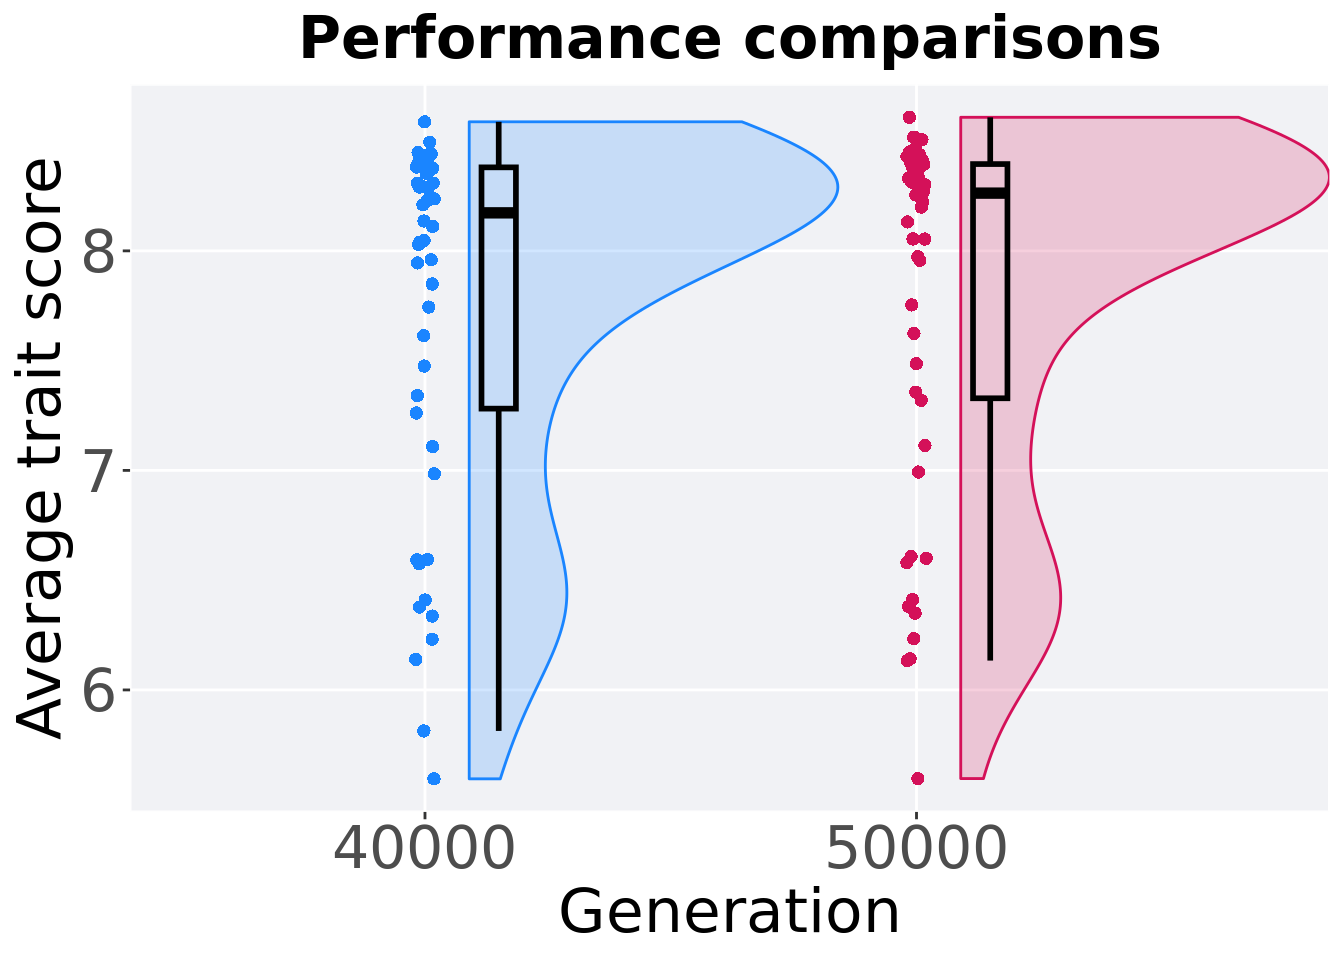
\includegraphics{mvc-diagnostics_files/figure-latex/ord-per-cmp-plt-tor-1.pdf}

Summary statistics for the best performance.

\begin{Shaded}
\begin{Highlighting}[]
\KeywordTok{filter}\NormalTok{(interval_df, acro }\OperatorTok{==}\StringTok{ 'tor'}\NormalTok{) }\OperatorTok
\StringTok{  }\KeywordTok{group_by}\NormalTok{(Generation) }\OperatorTok
\StringTok{  }\NormalTok{dplyr}\OperatorTok{::}\KeywordTok{summarise}\NormalTok{(}
    \DataTypeTok{count =} \KeywordTok{n}\NormalTok{(),}
    \DataTypeTok{na_cnt =} \KeywordTok{sum}\NormalTok{(}\KeywordTok{is.na}\NormalTok{(pop_fit_max)),}
    \DataTypeTok{min =} \KeywordTok{min}\NormalTok{(pop_fit_max }\OperatorTok{/}\StringTok{ }\NormalTok{DIMENSIONALITY, }\DataTypeTok{na.rm =} \OtherTok{TRUE}\NormalTok{),}
    \DataTypeTok{median =} \KeywordTok{median}\NormalTok{(pop_fit_max }\OperatorTok{/}\StringTok{ }\NormalTok{DIMENSIONALITY, }\DataTypeTok{na.rm =} \OtherTok{TRUE}\NormalTok{),}
    \DataTypeTok{mean =} \KeywordTok{mean}\NormalTok{(pop_fit_max }\OperatorTok{/}\StringTok{ }\NormalTok{DIMENSIONALITY, }\DataTypeTok{na.rm =} \OtherTok{TRUE}\NormalTok{),}
    \DataTypeTok{max =} \KeywordTok{max}\NormalTok{(pop_fit_max }\OperatorTok{/}\StringTok{ }\NormalTok{DIMENSIONALITY, }\DataTypeTok{na.rm =} \OtherTok{TRUE}\NormalTok{),}
    \DataTypeTok{IQR =} \KeywordTok{IQR}\NormalTok{(pop_fit_max }\OperatorTok{/}\StringTok{ }\NormalTok{DIMENSIONALITY, }\DataTypeTok{na.rm =} \OtherTok{TRUE}\NormalTok{)}
\NormalTok{  )}
\end{Highlighting}
\end{Shaded}

\begin{verbatim}
## # A tibble: 2 x 8
##   Generation count na_cnt   min median  mean   max   IQR
##   <fct>      <int>  <int> <dbl>  <dbl> <dbl> <dbl> <dbl>
## 1 40000         50      0  5.59   8.17  7.75  8.59  1.10
## 2 50000         50      0  5.60   8.26  7.79  8.61  1.07
\end{verbatim}

Results for post-hoc Wilcoxon rank-sum test.

\begin{Shaded}
\begin{Highlighting}[]
\KeywordTok{wilcox.test}\NormalTok{(}\DataTypeTok{x =} \KeywordTok{filter}\NormalTok{(interval_df, acro }\OperatorTok{==}\StringTok{ 'tor'} \OperatorTok{&}\StringTok{ }\NormalTok{Generation }\OperatorTok{==}\StringTok{ }\DecValTok{50000}\NormalTok{)}\OperatorTok{$}\NormalTok{pop_fit_max,}
            \DataTypeTok{y =} \KeywordTok{filter}\NormalTok{(interval_df, acro }\OperatorTok{==}\StringTok{ 'tor'} \OperatorTok{&}\StringTok{ }\NormalTok{Generation }\OperatorTok{==}\StringTok{ }\DecValTok{40000}\NormalTok{)}\OperatorTok{$}\NormalTok{pop_fit_max,}
            \DataTypeTok{alternative =} \StringTok{'t'}\NormalTok{)}
\end{Highlighting}
\end{Shaded}

\begin{verbatim}
## 
##  Wilcoxon rank sum test with continuity correction
## 
## data:  filter(interval_df, acro == "tor" & Generation == 50000)$pop_fit_max and filter(interval_df, acro == "tor" & Generation == 40000)$pop_fit_max
## W = 1343, p-value = 0.5237
## alternative hypothesis: true location shift is not equal to 0
\end{verbatim}

\hypertarget{lexicase-1}{%
\subsubsection{Lexicase}\label{lexicase-1}}

Plot for comparing performances at interval 40,000 \& 50,000.

\begin{Shaded}
\begin{Highlighting}[]
\KeywordTok{filter}\NormalTok{(interval_df, acro }\OperatorTok{==}\StringTok{ 'lex'}\NormalTok{) }\OperatorTok
\KeywordTok{ggplot}\NormalTok{(., }\KeywordTok{aes}\NormalTok{(}\DataTypeTok{x=}\NormalTok{Generation, }\DataTypeTok{y=}\NormalTok{pop_fit_max}\OperatorTok{/}\NormalTok{DIMENSIONALITY,}\DataTypeTok{fill=}\NormalTok{Generation,}\DataTypeTok{color=}\NormalTok{Generation,}\DataTypeTok{shape=}\NormalTok{Generation)) }\OperatorTok{+}
\StringTok{  }\KeywordTok{geom_flat_violin}\NormalTok{(}\DataTypeTok{position =} \KeywordTok{position_nudge}\NormalTok{(}\DataTypeTok{x =} \FloatTok{.09}\NormalTok{, }\DataTypeTok{y =} \DecValTok{0}\NormalTok{), }\DataTypeTok{scale =} \StringTok{'width'}\NormalTok{, }\DataTypeTok{alpha =} \FloatTok{0.2}\NormalTok{, }\DataTypeTok{width =} \FloatTok{1.5}\NormalTok{) }\OperatorTok{+}
\StringTok{  }\KeywordTok{geom_boxplot}\NormalTok{(}\DataTypeTok{color =} \StringTok{'black'}\NormalTok{, }\DataTypeTok{width =} \FloatTok{.07}\NormalTok{, }\DataTypeTok{outlier.shape =} \OtherTok{NA}\NormalTok{, }\DataTypeTok{alpha =} \FloatTok{0.0}\NormalTok{, }\DataTypeTok{size =} \FloatTok{1.0}\NormalTok{, }\DataTypeTok{position =} \KeywordTok{position_nudge}\NormalTok{(}\DataTypeTok{x =} \FloatTok{.15}\NormalTok{, }\DataTypeTok{y =} \DecValTok{0}\NormalTok{)) }\OperatorTok{+}
\StringTok{  }\KeywordTok{geom_point}\NormalTok{(}\DataTypeTok{position =} \KeywordTok{position_jitter}\NormalTok{(}\DataTypeTok{width =} \FloatTok{.02}\NormalTok{), }\DataTypeTok{size =} \FloatTok{2.0}\NormalTok{, }\DataTypeTok{alpha =} \FloatTok{1.0}\NormalTok{) }\OperatorTok{+}
\StringTok{    }\KeywordTok{scale_y_continuous}\NormalTok{(}
      \DataTypeTok{name=}\StringTok{"Average trait score"}\NormalTok{,}
\NormalTok{    ) }\OperatorTok{+}
\StringTok{    }\KeywordTok{scale_x_discrete}\NormalTok{(}
      \DataTypeTok{name=}\StringTok{"Generation"}
\NormalTok{    ) }\OperatorTok{+}
\StringTok{  }\KeywordTok{scale_shape_manual}\NormalTok{(}\DataTypeTok{values=}\KeywordTok{c}\NormalTok{(}\DecValTok{16}\NormalTok{,}\DecValTok{16}\NormalTok{))}\OperatorTok{+}
\StringTok{  }\KeywordTok{scale_colour_manual}\NormalTok{(}\DataTypeTok{values =}\NormalTok{ mvc_col, ) }\OperatorTok{+}
\StringTok{  }\KeywordTok{scale_fill_manual}\NormalTok{(}\DataTypeTok{values =}\NormalTok{ mvc_col) }\OperatorTok{+}
\StringTok{  }\KeywordTok{ggtitle}\NormalTok{(}\StringTok{'Performance comparisons'}\NormalTok{)}\OperatorTok{+}
\StringTok{  }\NormalTok{p_theme }\OperatorTok{+}\StringTok{ }\KeywordTok{theme}\NormalTok{(}\DataTypeTok{legend.position=}\StringTok{"none"}\NormalTok{)}
\end{Highlighting}
\end{Shaded}

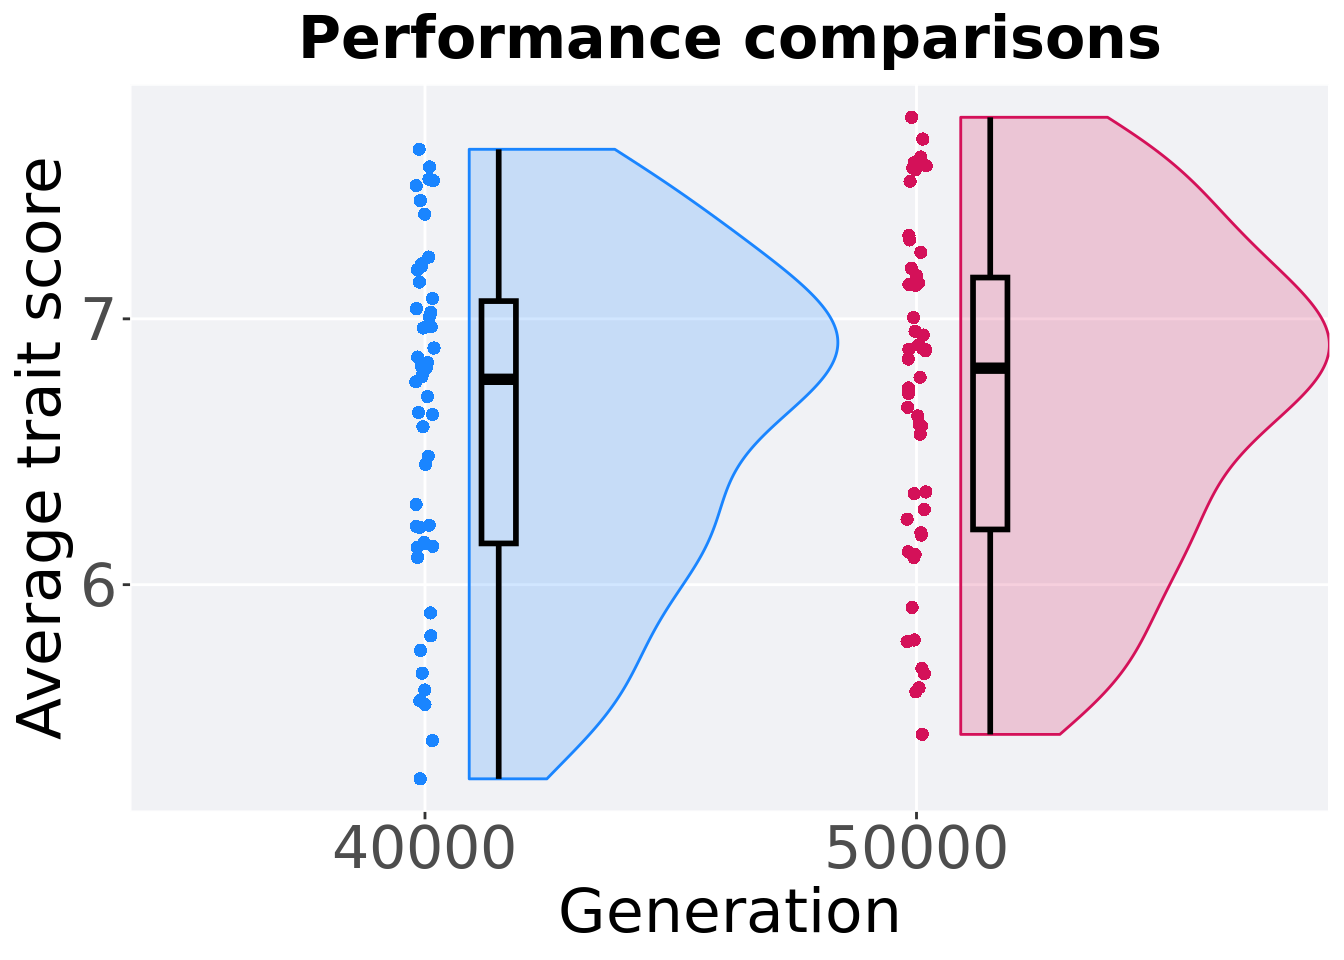
\includegraphics{mvc-diagnostics_files/figure-latex/ord-per-cmp-plt-lex-1.pdf}

Summary statistics for the best performance.

\begin{Shaded}
\begin{Highlighting}[]
\KeywordTok{filter}\NormalTok{(interval_df, acro }\OperatorTok{==}\StringTok{ 'lex'}\NormalTok{) }\OperatorTok
\StringTok{  }\KeywordTok{group_by}\NormalTok{(Generation) }\OperatorTok
\StringTok{  }\NormalTok{dplyr}\OperatorTok{::}\KeywordTok{summarise}\NormalTok{(}
    \DataTypeTok{count =} \KeywordTok{n}\NormalTok{(),}
    \DataTypeTok{na_cnt =} \KeywordTok{sum}\NormalTok{(}\KeywordTok{is.na}\NormalTok{(pop_fit_max)),}
    \DataTypeTok{min =} \KeywordTok{min}\NormalTok{(pop_fit_max }\OperatorTok{/}\StringTok{ }\NormalTok{DIMENSIONALITY, }\DataTypeTok{na.rm =} \OtherTok{TRUE}\NormalTok{),}
    \DataTypeTok{median =} \KeywordTok{median}\NormalTok{(pop_fit_max }\OperatorTok{/}\StringTok{ }\NormalTok{DIMENSIONALITY, }\DataTypeTok{na.rm =} \OtherTok{TRUE}\NormalTok{),}
    \DataTypeTok{mean =} \KeywordTok{mean}\NormalTok{(pop_fit_max }\OperatorTok{/}\StringTok{ }\NormalTok{DIMENSIONALITY, }\DataTypeTok{na.rm =} \OtherTok{TRUE}\NormalTok{),}
    \DataTypeTok{max =} \KeywordTok{max}\NormalTok{(pop_fit_max }\OperatorTok{/}\StringTok{ }\NormalTok{DIMENSIONALITY, }\DataTypeTok{na.rm =} \OtherTok{TRUE}\NormalTok{),}
    \DataTypeTok{IQR =} \KeywordTok{IQR}\NormalTok{(pop_fit_max }\OperatorTok{/}\StringTok{ }\NormalTok{DIMENSIONALITY, }\DataTypeTok{na.rm =} \OtherTok{TRUE}\NormalTok{)}
\NormalTok{  )}
\end{Highlighting}
\end{Shaded}

\begin{verbatim}
## # A tibble: 2 x 8
##   Generation count na_cnt   min median  mean   max   IQR
##   <fct>      <int>  <int> <dbl>  <dbl> <dbl> <dbl> <dbl>
## 1 40000         50      0  5.27   6.77  6.62  7.64 0.912
## 2 50000         50      0  5.44   6.81  6.71  7.76 0.948
\end{verbatim}

Results for post-hoc Wilcoxon rank-sum test.

\begin{Shaded}
\begin{Highlighting}[]
\KeywordTok{wilcox.test}\NormalTok{(}\DataTypeTok{x =} \KeywordTok{filter}\NormalTok{(interval_df, acro }\OperatorTok{==}\StringTok{ 'lex'} \OperatorTok{&}\StringTok{ }\NormalTok{Generation }\OperatorTok{==}\StringTok{ }\DecValTok{50000}\NormalTok{)}\OperatorTok{$}\NormalTok{pop_fit_max,}
            \DataTypeTok{y =} \KeywordTok{filter}\NormalTok{(interval_df, acro }\OperatorTok{==}\StringTok{ 'lex'} \OperatorTok{&}\StringTok{ }\NormalTok{Generation }\OperatorTok{==}\StringTok{ }\DecValTok{40000}\NormalTok{)}\OperatorTok{$}\NormalTok{pop_fit_max,}
            \DataTypeTok{alternative =} \StringTok{'t'}\NormalTok{)}
\end{Highlighting}
\end{Shaded}

\begin{verbatim}
## 
##  Wilcoxon rank sum test with continuity correction
## 
## data:  filter(interval_df, acro == "lex" & Generation == 50000)$pop_fit_max and filter(interval_df, acro == "lex" & Generation == 40000)$pop_fit_max
## W = 1346, p-value = 0.5103
## alternative hypothesis: true location shift is not equal to 0
\end{verbatim}

\hypertarget{genotypic-fitness-sharing-1}{%
\subsubsection{Genotypic fitness sharing}\label{genotypic-fitness-sharing-1}}

Plot for comparing performances at interval 40,000 \& 50,000.

\begin{Shaded}
\begin{Highlighting}[]
\KeywordTok{filter}\NormalTok{(interval_df, acro }\OperatorTok{==}\StringTok{ 'gfs'}\NormalTok{) }\OperatorTok
\KeywordTok{ggplot}\NormalTok{(., }\KeywordTok{aes}\NormalTok{(}\DataTypeTok{x=}\NormalTok{Generation, }\DataTypeTok{y=}\NormalTok{pop_fit_max}\OperatorTok{/}\NormalTok{DIMENSIONALITY,}\DataTypeTok{fill=}\NormalTok{Generation,}\DataTypeTok{color=}\NormalTok{Generation,}\DataTypeTok{shape=}\NormalTok{Generation)) }\OperatorTok{+}
\StringTok{  }\KeywordTok{geom_flat_violin}\NormalTok{(}\DataTypeTok{position =} \KeywordTok{position_nudge}\NormalTok{(}\DataTypeTok{x =} \FloatTok{.09}\NormalTok{, }\DataTypeTok{y =} \DecValTok{0}\NormalTok{), }\DataTypeTok{scale =} \StringTok{'width'}\NormalTok{, }\DataTypeTok{alpha =} \FloatTok{0.2}\NormalTok{, }\DataTypeTok{width =} \FloatTok{1.5}\NormalTok{) }\OperatorTok{+}
\StringTok{  }\KeywordTok{geom_boxplot}\NormalTok{(}\DataTypeTok{color =} \StringTok{'black'}\NormalTok{, }\DataTypeTok{width =} \FloatTok{.07}\NormalTok{, }\DataTypeTok{outlier.shape =} \OtherTok{NA}\NormalTok{, }\DataTypeTok{alpha =} \FloatTok{0.0}\NormalTok{, }\DataTypeTok{size =} \FloatTok{1.0}\NormalTok{, }\DataTypeTok{position =} \KeywordTok{position_nudge}\NormalTok{(}\DataTypeTok{x =} \FloatTok{.15}\NormalTok{, }\DataTypeTok{y =} \DecValTok{0}\NormalTok{)) }\OperatorTok{+}
\StringTok{  }\KeywordTok{geom_point}\NormalTok{(}\DataTypeTok{position =} \KeywordTok{position_jitter}\NormalTok{(}\DataTypeTok{width =} \FloatTok{.02}\NormalTok{), }\DataTypeTok{size =} \FloatTok{2.0}\NormalTok{, }\DataTypeTok{alpha =} \FloatTok{1.0}\NormalTok{) }\OperatorTok{+}
\StringTok{    }\KeywordTok{scale_y_continuous}\NormalTok{(}
      \DataTypeTok{name=}\StringTok{"Average trait score"}\NormalTok{,}
\NormalTok{    ) }\OperatorTok{+}
\StringTok{    }\KeywordTok{scale_x_discrete}\NormalTok{(}
      \DataTypeTok{name=}\StringTok{"Generation"}
\NormalTok{    ) }\OperatorTok{+}
\StringTok{  }\KeywordTok{scale_shape_manual}\NormalTok{(}\DataTypeTok{values=}\KeywordTok{c}\NormalTok{(}\DecValTok{16}\NormalTok{,}\DecValTok{16}\NormalTok{))}\OperatorTok{+}
\StringTok{  }\KeywordTok{scale_colour_manual}\NormalTok{(}\DataTypeTok{values =}\NormalTok{ mvc_col, ) }\OperatorTok{+}
\StringTok{  }\KeywordTok{scale_fill_manual}\NormalTok{(}\DataTypeTok{values =}\NormalTok{ mvc_col) }\OperatorTok{+}
\StringTok{  }\KeywordTok{ggtitle}\NormalTok{(}\StringTok{'Performance comparisons'}\NormalTok{)}\OperatorTok{+}
\StringTok{  }\NormalTok{p_theme }\OperatorTok{+}\StringTok{ }\KeywordTok{theme}\NormalTok{(}\DataTypeTok{legend.position=}\StringTok{"none"}\NormalTok{)}
\end{Highlighting}
\end{Shaded}

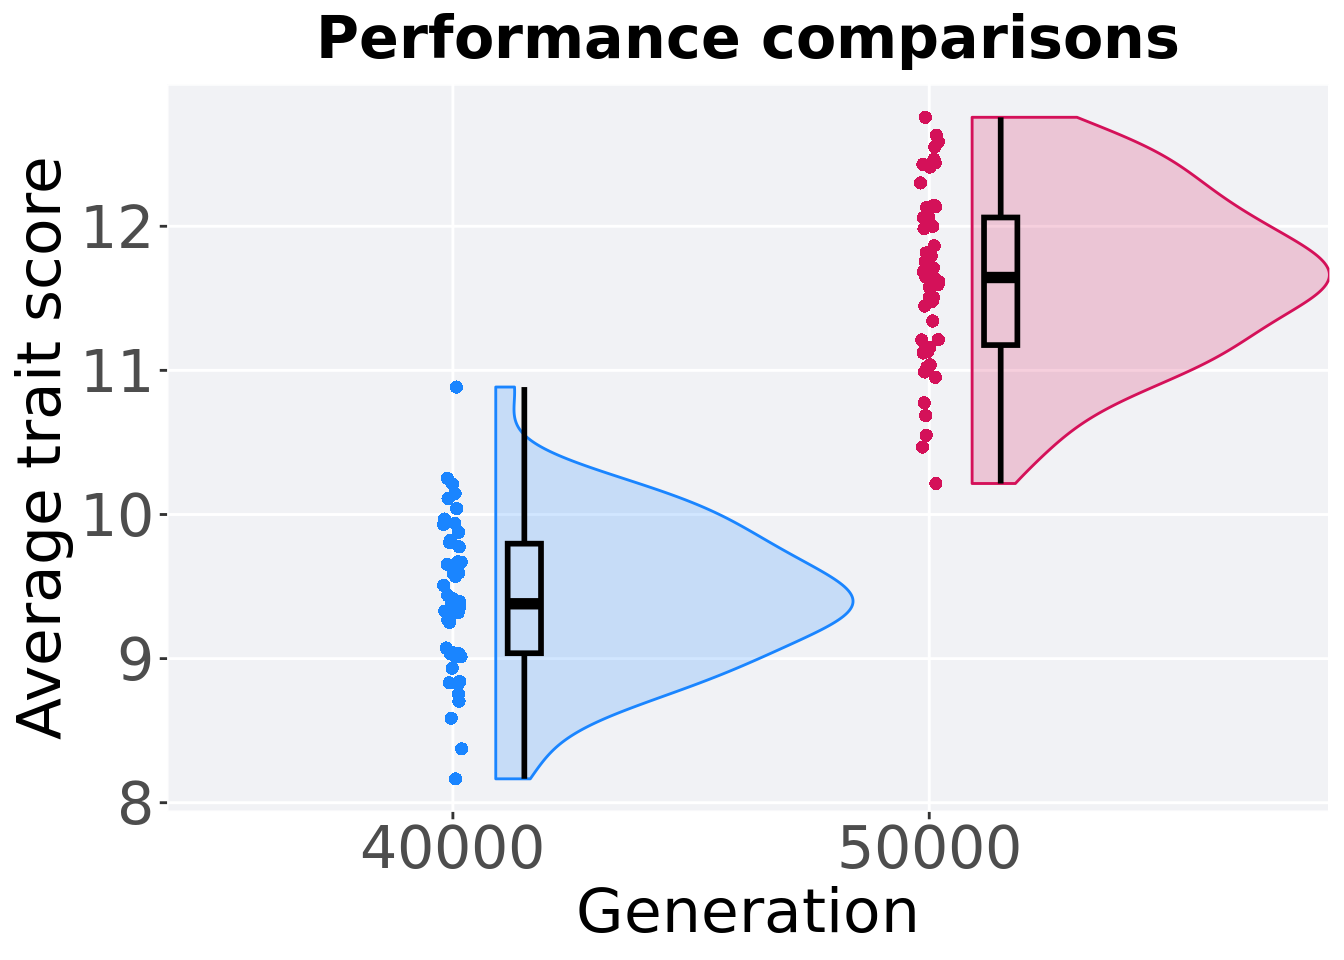
\includegraphics{mvc-diagnostics_files/figure-latex/ord-per-cmp-plt-gfs-1.pdf}

Summary statistics for the best performance.

\begin{Shaded}
\begin{Highlighting}[]
\KeywordTok{filter}\NormalTok{(interval_df, acro }\OperatorTok{==}\StringTok{ 'gfs'}\NormalTok{) }\OperatorTok
\StringTok{  }\KeywordTok{group_by}\NormalTok{(Generation) }\OperatorTok
\StringTok{  }\NormalTok{dplyr}\OperatorTok{::}\KeywordTok{summarise}\NormalTok{(}
    \DataTypeTok{count =} \KeywordTok{n}\NormalTok{(),}
    \DataTypeTok{na_cnt =} \KeywordTok{sum}\NormalTok{(}\KeywordTok{is.na}\NormalTok{(pop_fit_max)),}
    \DataTypeTok{min =} \KeywordTok{min}\NormalTok{(pop_fit_max }\OperatorTok{/}\StringTok{ }\NormalTok{DIMENSIONALITY, }\DataTypeTok{na.rm =} \OtherTok{TRUE}\NormalTok{),}
    \DataTypeTok{median =} \KeywordTok{median}\NormalTok{(pop_fit_max }\OperatorTok{/}\StringTok{ }\NormalTok{DIMENSIONALITY, }\DataTypeTok{na.rm =} \OtherTok{TRUE}\NormalTok{),}
    \DataTypeTok{mean =} \KeywordTok{mean}\NormalTok{(pop_fit_max }\OperatorTok{/}\StringTok{ }\NormalTok{DIMENSIONALITY, }\DataTypeTok{na.rm =} \OtherTok{TRUE}\NormalTok{),}
    \DataTypeTok{max =} \KeywordTok{max}\NormalTok{(pop_fit_max }\OperatorTok{/}\StringTok{ }\NormalTok{DIMENSIONALITY, }\DataTypeTok{na.rm =} \OtherTok{TRUE}\NormalTok{),}
    \DataTypeTok{IQR =} \KeywordTok{IQR}\NormalTok{(pop_fit_max }\OperatorTok{/}\StringTok{ }\NormalTok{DIMENSIONALITY, }\DataTypeTok{na.rm =} \OtherTok{TRUE}\NormalTok{)}
\NormalTok{  )}
\end{Highlighting}
\end{Shaded}

\begin{verbatim}
## # A tibble: 2 x 8
##   Generation count na_cnt   min median  mean   max   IQR
##   <fct>      <int>  <int> <dbl>  <dbl> <dbl> <dbl> <dbl>
## 1 40000         50      0  8.17   9.38  9.43  10.9 0.760
## 2 50000         50      0 10.2   11.6  11.6   12.8 0.885
\end{verbatim}

Results for post-hoc Wilcoxon rank-sum test.

\begin{Shaded}
\begin{Highlighting}[]
\KeywordTok{wilcox.test}\NormalTok{(}\DataTypeTok{x =} \KeywordTok{filter}\NormalTok{(interval_df, acro }\OperatorTok{==}\StringTok{ 'gfs'} \OperatorTok{&}\StringTok{ }\NormalTok{Generation }\OperatorTok{==}\StringTok{ }\DecValTok{50000}\NormalTok{)}\OperatorTok{$}\NormalTok{pop_fit_max,}
            \DataTypeTok{y =} \KeywordTok{filter}\NormalTok{(interval_df, acro }\OperatorTok{==}\StringTok{ 'gfs'} \OperatorTok{&}\StringTok{ }\NormalTok{Generation }\OperatorTok{==}\StringTok{ }\DecValTok{40000}\NormalTok{)}\OperatorTok{$}\NormalTok{pop_fit_max,}
            \DataTypeTok{alternative =} \StringTok{'g'}\NormalTok{)}
\end{Highlighting}
\end{Shaded}

\begin{verbatim}
## 
##  Wilcoxon rank sum test with continuity correction
## 
## data:  filter(interval_df, acro == "gfs" & Generation == 50000)$pop_fit_max and filter(interval_df, acro == "gfs" & Generation == 40000)$pop_fit_max
## W = 2494, p-value < 2.2e-16
## alternative hypothesis: true location shift is greater than 0
\end{verbatim}

\hypertarget{phenotypic-fitness-sharing-1}{%
\subsubsection{Phenotypic fitness sharing}\label{phenotypic-fitness-sharing-1}}

Plot for comparing performances at interval 40,000 \& 50,000.

\begin{Shaded}
\begin{Highlighting}[]
\KeywordTok{filter}\NormalTok{(interval_df, acro }\OperatorTok{==}\StringTok{ 'pfs'}\NormalTok{) }\OperatorTok
\KeywordTok{ggplot}\NormalTok{(., }\KeywordTok{aes}\NormalTok{(}\DataTypeTok{x=}\NormalTok{Generation, }\DataTypeTok{y=}\NormalTok{pop_fit_max}\OperatorTok{/}\NormalTok{DIMENSIONALITY,}\DataTypeTok{fill=}\NormalTok{Generation,}\DataTypeTok{color=}\NormalTok{Generation,}\DataTypeTok{shape=}\NormalTok{Generation)) }\OperatorTok{+}
\StringTok{  }\KeywordTok{geom_flat_violin}\NormalTok{(}\DataTypeTok{position =} \KeywordTok{position_nudge}\NormalTok{(}\DataTypeTok{x =} \FloatTok{.09}\NormalTok{, }\DataTypeTok{y =} \DecValTok{0}\NormalTok{), }\DataTypeTok{scale =} \StringTok{'width'}\NormalTok{, }\DataTypeTok{alpha =} \FloatTok{0.2}\NormalTok{, }\DataTypeTok{width =} \FloatTok{1.5}\NormalTok{) }\OperatorTok{+}
\StringTok{  }\KeywordTok{geom_boxplot}\NormalTok{(}\DataTypeTok{color =} \StringTok{'black'}\NormalTok{, }\DataTypeTok{width =} \FloatTok{.07}\NormalTok{, }\DataTypeTok{outlier.shape =} \OtherTok{NA}\NormalTok{, }\DataTypeTok{alpha =} \FloatTok{0.0}\NormalTok{, }\DataTypeTok{size =} \FloatTok{1.0}\NormalTok{, }\DataTypeTok{position =} \KeywordTok{position_nudge}\NormalTok{(}\DataTypeTok{x =} \FloatTok{.15}\NormalTok{, }\DataTypeTok{y =} \DecValTok{0}\NormalTok{)) }\OperatorTok{+}
\StringTok{  }\KeywordTok{geom_point}\NormalTok{(}\DataTypeTok{position =} \KeywordTok{position_jitter}\NormalTok{(}\DataTypeTok{width =} \FloatTok{.02}\NormalTok{), }\DataTypeTok{size =} \FloatTok{2.0}\NormalTok{, }\DataTypeTok{alpha =} \FloatTok{1.0}\NormalTok{) }\OperatorTok{+}
\StringTok{    }\KeywordTok{scale_y_continuous}\NormalTok{(}
      \DataTypeTok{name=}\StringTok{"Average trait score"}\NormalTok{,}
\NormalTok{    ) }\OperatorTok{+}
\StringTok{    }\KeywordTok{scale_x_discrete}\NormalTok{(}
      \DataTypeTok{name=}\StringTok{"Generation"}
\NormalTok{    ) }\OperatorTok{+}
\StringTok{  }\KeywordTok{scale_shape_manual}\NormalTok{(}\DataTypeTok{values=}\KeywordTok{c}\NormalTok{(}\DecValTok{16}\NormalTok{,}\DecValTok{16}\NormalTok{))}\OperatorTok{+}
\StringTok{  }\KeywordTok{scale_colour_manual}\NormalTok{(}\DataTypeTok{values =}\NormalTok{ mvc_col, ) }\OperatorTok{+}
\StringTok{  }\KeywordTok{scale_fill_manual}\NormalTok{(}\DataTypeTok{values =}\NormalTok{ mvc_col) }\OperatorTok{+}
\StringTok{  }\KeywordTok{ggtitle}\NormalTok{(}\StringTok{'Performance comparisons'}\NormalTok{)}\OperatorTok{+}
\StringTok{  }\NormalTok{p_theme }\OperatorTok{+}\StringTok{ }\KeywordTok{theme}\NormalTok{(}\DataTypeTok{legend.position=}\StringTok{"none"}\NormalTok{)}
\end{Highlighting}
\end{Shaded}

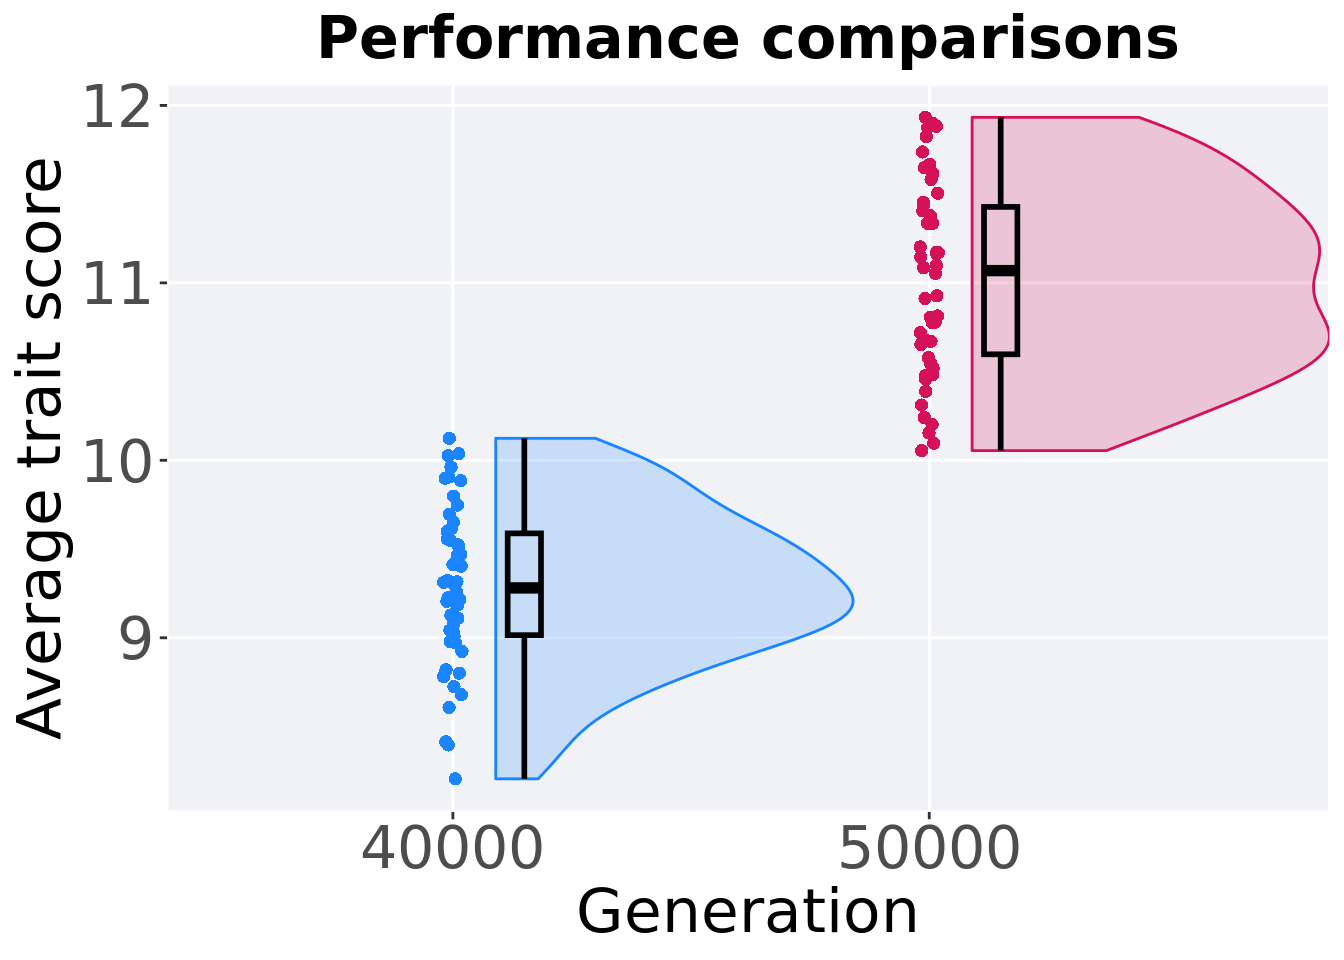
\includegraphics{mvc-diagnostics_files/figure-latex/ord-per-cmp-plt-pfs-1.pdf}

Summary statistics for the best performance.

\begin{Shaded}
\begin{Highlighting}[]
\KeywordTok{filter}\NormalTok{(interval_df, acro }\OperatorTok{==}\StringTok{ 'pfs'}\NormalTok{) }\OperatorTok
\StringTok{  }\KeywordTok{group_by}\NormalTok{(Generation) }\OperatorTok
\StringTok{  }\NormalTok{dplyr}\OperatorTok{::}\KeywordTok{summarise}\NormalTok{(}
    \DataTypeTok{count =} \KeywordTok{n}\NormalTok{(),}
    \DataTypeTok{na_cnt =} \KeywordTok{sum}\NormalTok{(}\KeywordTok{is.na}\NormalTok{(pop_fit_max)),}
    \DataTypeTok{min =} \KeywordTok{min}\NormalTok{(pop_fit_max }\OperatorTok{/}\StringTok{ }\NormalTok{DIMENSIONALITY, }\DataTypeTok{na.rm =} \OtherTok{TRUE}\NormalTok{),}
    \DataTypeTok{median =} \KeywordTok{median}\NormalTok{(pop_fit_max }\OperatorTok{/}\StringTok{ }\NormalTok{DIMENSIONALITY, }\DataTypeTok{na.rm =} \OtherTok{TRUE}\NormalTok{),}
    \DataTypeTok{mean =} \KeywordTok{mean}\NormalTok{(pop_fit_max }\OperatorTok{/}\StringTok{ }\NormalTok{DIMENSIONALITY, }\DataTypeTok{na.rm =} \OtherTok{TRUE}\NormalTok{),}
    \DataTypeTok{max =} \KeywordTok{max}\NormalTok{(pop_fit_max }\OperatorTok{/}\StringTok{ }\NormalTok{DIMENSIONALITY, }\DataTypeTok{na.rm =} \OtherTok{TRUE}\NormalTok{),}
    \DataTypeTok{IQR =} \KeywordTok{IQR}\NormalTok{(pop_fit_max }\OperatorTok{/}\StringTok{ }\NormalTok{DIMENSIONALITY, }\DataTypeTok{na.rm =} \OtherTok{TRUE}\NormalTok{)}
\NormalTok{  )}
\end{Highlighting}
\end{Shaded}

\begin{verbatim}
## # A tibble: 2 x 8
##   Generation count na_cnt   min median  mean   max   IQR
##   <fct>      <int>  <int> <dbl>  <dbl> <dbl> <dbl> <dbl>
## 1 40000         50      0  8.20   9.28  9.28  10.1 0.574
## 2 50000         50      0 10.1   11.1  11.0   11.9 0.831
\end{verbatim}

Results for post-hoc Wilcoxon rank-sum test.

\begin{Shaded}
\begin{Highlighting}[]
\KeywordTok{wilcox.test}\NormalTok{(}\DataTypeTok{x =} \KeywordTok{filter}\NormalTok{(interval_df, acro }\OperatorTok{==}\StringTok{ 'pfs'} \OperatorTok{&}\StringTok{ }\NormalTok{Generation }\OperatorTok{==}\StringTok{ }\DecValTok{50000}\NormalTok{)}\OperatorTok{$}\NormalTok{pop_fit_max,}
            \DataTypeTok{y =} \KeywordTok{filter}\NormalTok{(interval_df, acro }\OperatorTok{==}\StringTok{ 'pfs'} \OperatorTok{&}\StringTok{ }\NormalTok{Generation }\OperatorTok{==}\StringTok{ }\DecValTok{40000}\NormalTok{)}\OperatorTok{$}\NormalTok{pop_fit_max,}
            \DataTypeTok{alternative =} \StringTok{'g'}\NormalTok{)}
\end{Highlighting}
\end{Shaded}

\begin{verbatim}
## 
##  Wilcoxon rank sum test with continuity correction
## 
## data:  filter(interval_df, acro == "pfs" & Generation == 50000)$pop_fit_max and filter(interval_df, acro == "pfs" & Generation == 40000)$pop_fit_max
## W = 2498, p-value < 2.2e-16
## alternative hypothesis: true location shift is greater than 0
\end{verbatim}

\hypertarget{nondominated-sorting-1}{%
\subsubsection{Nondominated sorting}\label{nondominated-sorting-1}}

Plot for comparing performances at interval 40,000 \& 50,000.

\begin{Shaded}
\begin{Highlighting}[]
\KeywordTok{filter}\NormalTok{(interval_df, acro }\OperatorTok{==}\StringTok{ 'nds'}\NormalTok{) }\OperatorTok
\KeywordTok{ggplot}\NormalTok{(., }\KeywordTok{aes}\NormalTok{(}\DataTypeTok{x=}\NormalTok{Generation, }\DataTypeTok{y=}\NormalTok{pop_fit_max}\OperatorTok{/}\NormalTok{DIMENSIONALITY,}\DataTypeTok{fill=}\NormalTok{Generation,}\DataTypeTok{color=}\NormalTok{Generation,}\DataTypeTok{shape=}\NormalTok{Generation)) }\OperatorTok{+}
\StringTok{  }\KeywordTok{geom_flat_violin}\NormalTok{(}\DataTypeTok{position =} \KeywordTok{position_nudge}\NormalTok{(}\DataTypeTok{x =} \FloatTok{.09}\NormalTok{, }\DataTypeTok{y =} \DecValTok{0}\NormalTok{), }\DataTypeTok{scale =} \StringTok{'width'}\NormalTok{, }\DataTypeTok{alpha =} \FloatTok{0.2}\NormalTok{, }\DataTypeTok{width =} \FloatTok{1.5}\NormalTok{) }\OperatorTok{+}
\StringTok{  }\KeywordTok{geom_boxplot}\NormalTok{(}\DataTypeTok{color =} \StringTok{'black'}\NormalTok{, }\DataTypeTok{width =} \FloatTok{.07}\NormalTok{, }\DataTypeTok{outlier.shape =} \OtherTok{NA}\NormalTok{, }\DataTypeTok{alpha =} \FloatTok{0.0}\NormalTok{, }\DataTypeTok{size =} \FloatTok{1.0}\NormalTok{, }\DataTypeTok{position =} \KeywordTok{position_nudge}\NormalTok{(}\DataTypeTok{x =} \FloatTok{.15}\NormalTok{, }\DataTypeTok{y =} \DecValTok{0}\NormalTok{)) }\OperatorTok{+}
\StringTok{  }\KeywordTok{geom_point}\NormalTok{(}\DataTypeTok{position =} \KeywordTok{position_jitter}\NormalTok{(}\DataTypeTok{width =} \FloatTok{.02}\NormalTok{), }\DataTypeTok{size =} \FloatTok{2.0}\NormalTok{, }\DataTypeTok{alpha =} \FloatTok{1.0}\NormalTok{) }\OperatorTok{+}
\StringTok{    }\KeywordTok{scale_y_continuous}\NormalTok{(}
      \DataTypeTok{name=}\StringTok{"Average trait score"}\NormalTok{,}
\NormalTok{    ) }\OperatorTok{+}
\StringTok{    }\KeywordTok{scale_x_discrete}\NormalTok{(}
      \DataTypeTok{name=}\StringTok{"Generation"}
\NormalTok{    ) }\OperatorTok{+}
\StringTok{  }\KeywordTok{scale_shape_manual}\NormalTok{(}\DataTypeTok{values=}\KeywordTok{c}\NormalTok{(}\DecValTok{16}\NormalTok{,}\DecValTok{16}\NormalTok{))}\OperatorTok{+}
\StringTok{  }\KeywordTok{scale_colour_manual}\NormalTok{(}\DataTypeTok{values =}\NormalTok{ mvc_col, ) }\OperatorTok{+}
\StringTok{  }\KeywordTok{scale_fill_manual}\NormalTok{(}\DataTypeTok{values =}\NormalTok{ mvc_col) }\OperatorTok{+}
\StringTok{  }\KeywordTok{ggtitle}\NormalTok{(}\StringTok{'Performance comparisons'}\NormalTok{)}\OperatorTok{+}
\StringTok{  }\NormalTok{p_theme }\OperatorTok{+}\StringTok{ }\KeywordTok{theme}\NormalTok{(}\DataTypeTok{legend.position=}\StringTok{"none"}\NormalTok{)}
\end{Highlighting}
\end{Shaded}

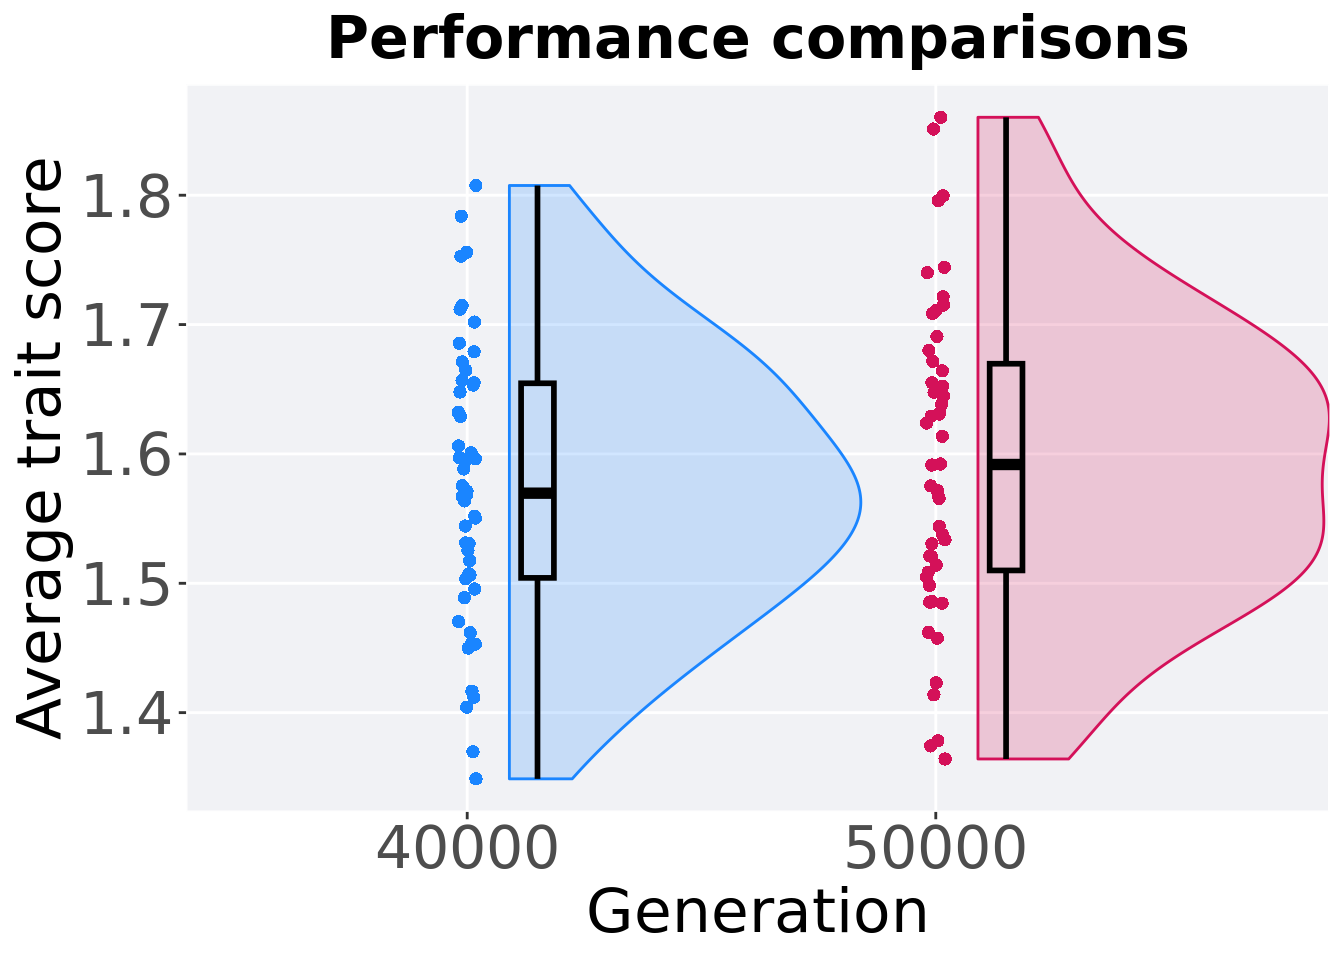
\includegraphics{mvc-diagnostics_files/figure-latex/ord-per-cmp-plt-nds-1.pdf}

Summary statistics for the best performance.

\begin{Shaded}
\begin{Highlighting}[]
\KeywordTok{filter}\NormalTok{(interval_df, acro }\OperatorTok{==}\StringTok{ 'nds'}\NormalTok{) }\OperatorTok
\StringTok{  }\KeywordTok{group_by}\NormalTok{(Generation) }\OperatorTok
\StringTok{  }\NormalTok{dplyr}\OperatorTok{::}\KeywordTok{summarise}\NormalTok{(}
    \DataTypeTok{count =} \KeywordTok{n}\NormalTok{(),}
    \DataTypeTok{na_cnt =} \KeywordTok{sum}\NormalTok{(}\KeywordTok{is.na}\NormalTok{(pop_fit_max)),}
    \DataTypeTok{min =} \KeywordTok{min}\NormalTok{(pop_fit_max }\OperatorTok{/}\StringTok{ }\NormalTok{DIMENSIONALITY, }\DataTypeTok{na.rm =} \OtherTok{TRUE}\NormalTok{),}
    \DataTypeTok{median =} \KeywordTok{median}\NormalTok{(pop_fit_max }\OperatorTok{/}\StringTok{ }\NormalTok{DIMENSIONALITY, }\DataTypeTok{na.rm =} \OtherTok{TRUE}\NormalTok{),}
    \DataTypeTok{mean =} \KeywordTok{mean}\NormalTok{(pop_fit_max }\OperatorTok{/}\StringTok{ }\NormalTok{DIMENSIONALITY, }\DataTypeTok{na.rm =} \OtherTok{TRUE}\NormalTok{),}
    \DataTypeTok{max =} \KeywordTok{max}\NormalTok{(pop_fit_max }\OperatorTok{/}\StringTok{ }\NormalTok{DIMENSIONALITY, }\DataTypeTok{na.rm =} \OtherTok{TRUE}\NormalTok{),}
    \DataTypeTok{IQR =} \KeywordTok{IQR}\NormalTok{(pop_fit_max }\OperatorTok{/}\StringTok{ }\NormalTok{DIMENSIONALITY, }\DataTypeTok{na.rm =} \OtherTok{TRUE}\NormalTok{)}
\NormalTok{  )}
\end{Highlighting}
\end{Shaded}

\begin{verbatim}
## # A tibble: 2 x 8
##   Generation count na_cnt   min median  mean   max   IQR
##   <fct>      <int>  <int> <dbl>  <dbl> <dbl> <dbl> <dbl>
## 1 40000         50      0  1.35   1.57  1.57  1.81 0.150
## 2 50000         50      0  1.36   1.59  1.59  1.86 0.160
\end{verbatim}

Results for post-hoc Wilcoxon rank-sum test.

\begin{Shaded}
\begin{Highlighting}[]
\KeywordTok{wilcox.test}\NormalTok{(}\DataTypeTok{x =} \KeywordTok{filter}\NormalTok{(interval_df, acro }\OperatorTok{==}\StringTok{ 'nds'} \OperatorTok{&}\StringTok{ }\NormalTok{Generation }\OperatorTok{==}\StringTok{ }\DecValTok{50000}\NormalTok{)}\OperatorTok{$}\NormalTok{pop_fit_max,}
            \DataTypeTok{y =} \KeywordTok{filter}\NormalTok{(interval_df, acro }\OperatorTok{==}\StringTok{ 'nds'} \OperatorTok{&}\StringTok{ }\NormalTok{Generation }\OperatorTok{==}\StringTok{ }\DecValTok{40000}\NormalTok{)}\OperatorTok{$}\NormalTok{pop_fit_max,}
            \DataTypeTok{alternative =} \StringTok{'t'}\NormalTok{)}
\end{Highlighting}
\end{Shaded}

\begin{verbatim}
## 
##  Wilcoxon rank sum test with continuity correction
## 
## data:  filter(interval_df, acro == "nds" & Generation == 50000)$pop_fit_max and filter(interval_df, acro == "nds" & Generation == 40000)$pop_fit_max
## W = 1359, p-value = 0.4545
## alternative hypothesis: true location shift is not equal to 0
\end{verbatim}

\hypertarget{novelty-search-1}{%
\subsubsection{Novelty search}\label{novelty-search-1}}

Plot for comparing performances at interval 40,000 \& 50,000.

\begin{Shaded}
\begin{Highlighting}[]
\KeywordTok{filter}\NormalTok{(interval_df, acro }\OperatorTok{==}\StringTok{ 'nov'}\NormalTok{) }\OperatorTok
\KeywordTok{ggplot}\NormalTok{(., }\KeywordTok{aes}\NormalTok{(}\DataTypeTok{x=}\NormalTok{Generation, }\DataTypeTok{y=}\NormalTok{pop_fit_max}\OperatorTok{/}\NormalTok{DIMENSIONALITY,}\DataTypeTok{fill=}\NormalTok{Generation,}\DataTypeTok{color=}\NormalTok{Generation,}\DataTypeTok{shape=}\NormalTok{Generation)) }\OperatorTok{+}
\StringTok{  }\KeywordTok{geom_flat_violin}\NormalTok{(}\DataTypeTok{position =} \KeywordTok{position_nudge}\NormalTok{(}\DataTypeTok{x =} \FloatTok{.09}\NormalTok{, }\DataTypeTok{y =} \DecValTok{0}\NormalTok{), }\DataTypeTok{scale =} \StringTok{'width'}\NormalTok{, }\DataTypeTok{alpha =} \FloatTok{0.2}\NormalTok{, }\DataTypeTok{width =} \FloatTok{1.5}\NormalTok{) }\OperatorTok{+}
\StringTok{  }\KeywordTok{geom_boxplot}\NormalTok{(}\DataTypeTok{color =} \StringTok{'black'}\NormalTok{, }\DataTypeTok{width =} \FloatTok{.07}\NormalTok{, }\DataTypeTok{outlier.shape =} \OtherTok{NA}\NormalTok{, }\DataTypeTok{alpha =} \FloatTok{0.0}\NormalTok{, }\DataTypeTok{size =} \FloatTok{1.0}\NormalTok{, }\DataTypeTok{position =} \KeywordTok{position_nudge}\NormalTok{(}\DataTypeTok{x =} \FloatTok{.15}\NormalTok{, }\DataTypeTok{y =} \DecValTok{0}\NormalTok{)) }\OperatorTok{+}
\StringTok{  }\KeywordTok{geom_point}\NormalTok{(}\DataTypeTok{position =} \KeywordTok{position_jitter}\NormalTok{(}\DataTypeTok{width =} \FloatTok{.02}\NormalTok{), }\DataTypeTok{size =} \FloatTok{2.0}\NormalTok{, }\DataTypeTok{alpha =} \FloatTok{1.0}\NormalTok{) }\OperatorTok{+}
\StringTok{    }\KeywordTok{scale_y_continuous}\NormalTok{(}
      \DataTypeTok{name=}\StringTok{"Average trait score"}\NormalTok{,}
\NormalTok{    ) }\OperatorTok{+}
\StringTok{    }\KeywordTok{scale_x_discrete}\NormalTok{(}
      \DataTypeTok{name=}\StringTok{"Generation"}
\NormalTok{    ) }\OperatorTok{+}
\StringTok{  }\KeywordTok{scale_shape_manual}\NormalTok{(}\DataTypeTok{values=}\KeywordTok{c}\NormalTok{(}\DecValTok{16}\NormalTok{,}\DecValTok{16}\NormalTok{))}\OperatorTok{+}
\StringTok{  }\KeywordTok{scale_colour_manual}\NormalTok{(}\DataTypeTok{values =}\NormalTok{ mvc_col, ) }\OperatorTok{+}
\StringTok{  }\KeywordTok{scale_fill_manual}\NormalTok{(}\DataTypeTok{values =}\NormalTok{ mvc_col) }\OperatorTok{+}
\StringTok{  }\KeywordTok{ggtitle}\NormalTok{(}\StringTok{'Performance comparisons'}\NormalTok{)}\OperatorTok{+}
\StringTok{  }\NormalTok{p_theme }\OperatorTok{+}\StringTok{ }\KeywordTok{theme}\NormalTok{(}\DataTypeTok{legend.position=}\StringTok{"none"}\NormalTok{)}
\end{Highlighting}
\end{Shaded}

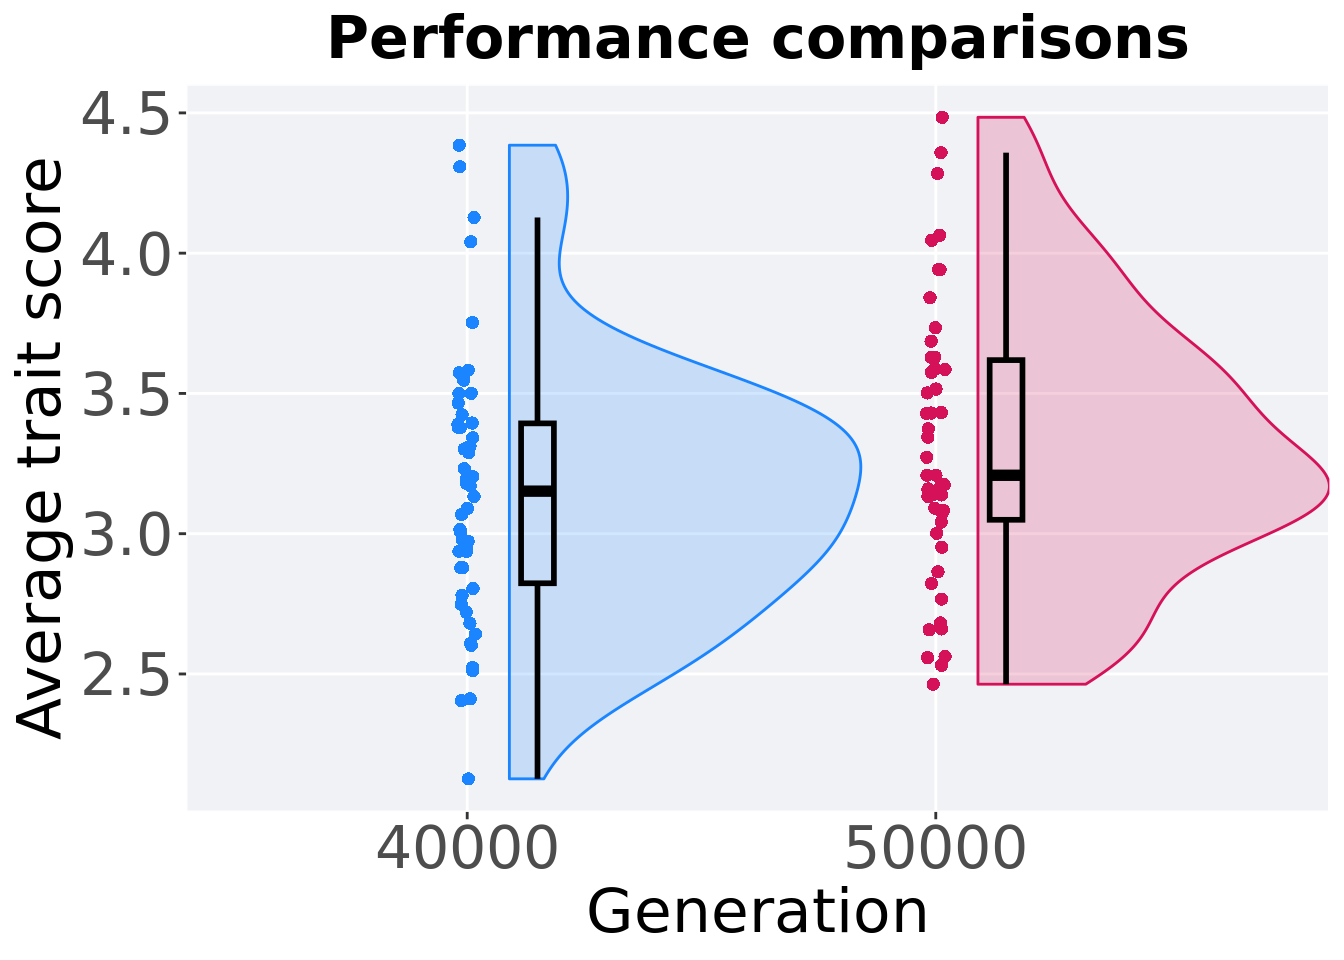
\includegraphics{mvc-diagnostics_files/figure-latex/ord-per-cmp-plt-nov-1.pdf}

Summary statistics for the best performance.

\begin{Shaded}
\begin{Highlighting}[]
\KeywordTok{filter}\NormalTok{(interval_df, acro }\OperatorTok{==}\StringTok{ 'nov'}\NormalTok{) }\OperatorTok
\StringTok{  }\KeywordTok{group_by}\NormalTok{(Generation) }\OperatorTok
\StringTok{  }\NormalTok{dplyr}\OperatorTok{::}\KeywordTok{summarise}\NormalTok{(}
    \DataTypeTok{count =} \KeywordTok{n}\NormalTok{(),}
    \DataTypeTok{na_cnt =} \KeywordTok{sum}\NormalTok{(}\KeywordTok{is.na}\NormalTok{(pop_fit_max)),}
    \DataTypeTok{min =} \KeywordTok{min}\NormalTok{(pop_fit_max }\OperatorTok{/}\StringTok{ }\NormalTok{DIMENSIONALITY, }\DataTypeTok{na.rm =} \OtherTok{TRUE}\NormalTok{),}
    \DataTypeTok{median =} \KeywordTok{median}\NormalTok{(pop_fit_max }\OperatorTok{/}\StringTok{ }\NormalTok{DIMENSIONALITY, }\DataTypeTok{na.rm =} \OtherTok{TRUE}\NormalTok{),}
    \DataTypeTok{mean =} \KeywordTok{mean}\NormalTok{(pop_fit_max }\OperatorTok{/}\StringTok{ }\NormalTok{DIMENSIONALITY, }\DataTypeTok{na.rm =} \OtherTok{TRUE}\NormalTok{),}
    \DataTypeTok{max =} \KeywordTok{max}\NormalTok{(pop_fit_max }\OperatorTok{/}\StringTok{ }\NormalTok{DIMENSIONALITY, }\DataTypeTok{na.rm =} \OtherTok{TRUE}\NormalTok{),}
    \DataTypeTok{IQR =} \KeywordTok{IQR}\NormalTok{(pop_fit_max }\OperatorTok{/}\StringTok{ }\NormalTok{DIMENSIONALITY, }\DataTypeTok{na.rm =} \OtherTok{TRUE}\NormalTok{)}
\NormalTok{  )}
\end{Highlighting}
\end{Shaded}

\begin{verbatim}
## # A tibble: 2 x 8
##   Generation count na_cnt   min median  mean   max   IQR
##   <fct>      <int>  <int> <dbl>  <dbl> <dbl> <dbl> <dbl>
## 1 40000         50      0  2.13   3.15  3.15  4.38 0.570
## 2 50000         50      0  2.46   3.21  3.32  4.48 0.569
\end{verbatim}

Results for post-hoc Wilcoxon rank-sum test.

\begin{Shaded}
\begin{Highlighting}[]
\KeywordTok{wilcox.test}\NormalTok{(}\DataTypeTok{x =} \KeywordTok{filter}\NormalTok{(interval_df, acro }\OperatorTok{==}\StringTok{ 'nov'} \OperatorTok{&}\StringTok{ }\NormalTok{Generation }\OperatorTok{==}\StringTok{ }\DecValTok{50000}\NormalTok{)}\OperatorTok{$}\NormalTok{pop_fit_max,}
            \DataTypeTok{y =} \KeywordTok{filter}\NormalTok{(interval_df, acro }\OperatorTok{==}\StringTok{ 'nov'} \OperatorTok{&}\StringTok{ }\NormalTok{Generation }\OperatorTok{==}\StringTok{ }\DecValTok{40000}\NormalTok{)}\OperatorTok{$}\NormalTok{pop_fit_max,}
            \DataTypeTok{alternative =} \StringTok{'t'}\NormalTok{)}
\end{Highlighting}
\end{Shaded}

\begin{verbatim}
## 
##  Wilcoxon rank sum test with continuity correction
## 
## data:  filter(interval_df, acro == "nov" & Generation == 50000)$pop_fit_max and filter(interval_df, acro == "nov" & Generation == 40000)$pop_fit_max
## W = 1506, p-value = 0.07818
## alternative hypothesis: true location shift is not equal to 0
\end{verbatim}

\hypertarget{random-1}{%
\subsubsection{Random}\label{random-1}}

Plot for comparing performances at interval 40,000 \& 50,000.

\begin{Shaded}
\begin{Highlighting}[]
\KeywordTok{filter}\NormalTok{(interval_df, acro }\OperatorTok{==}\StringTok{ 'ran'}\NormalTok{) }\OperatorTok
\KeywordTok{ggplot}\NormalTok{(., }\KeywordTok{aes}\NormalTok{(}\DataTypeTok{x=}\NormalTok{Generation, }\DataTypeTok{y=}\NormalTok{pop_fit_max}\OperatorTok{/}\NormalTok{DIMENSIONALITY,}\DataTypeTok{fill=}\NormalTok{Generation,}\DataTypeTok{color=}\NormalTok{Generation,}\DataTypeTok{shape=}\NormalTok{Generation)) }\OperatorTok{+}
\StringTok{  }\KeywordTok{geom_flat_violin}\NormalTok{(}\DataTypeTok{position =} \KeywordTok{position_nudge}\NormalTok{(}\DataTypeTok{x =} \FloatTok{.09}\NormalTok{, }\DataTypeTok{y =} \DecValTok{0}\NormalTok{), }\DataTypeTok{scale =} \StringTok{'width'}\NormalTok{, }\DataTypeTok{alpha =} \FloatTok{0.2}\NormalTok{, }\DataTypeTok{width =} \FloatTok{1.5}\NormalTok{) }\OperatorTok{+}
\StringTok{  }\KeywordTok{geom_boxplot}\NormalTok{(}\DataTypeTok{color =} \StringTok{'black'}\NormalTok{, }\DataTypeTok{width =} \FloatTok{.07}\NormalTok{, }\DataTypeTok{outlier.shape =} \OtherTok{NA}\NormalTok{, }\DataTypeTok{alpha =} \FloatTok{0.0}\NormalTok{, }\DataTypeTok{size =} \FloatTok{1.0}\NormalTok{, }\DataTypeTok{position =} \KeywordTok{position_nudge}\NormalTok{(}\DataTypeTok{x =} \FloatTok{.15}\NormalTok{, }\DataTypeTok{y =} \DecValTok{0}\NormalTok{)) }\OperatorTok{+}
\StringTok{  }\KeywordTok{geom_point}\NormalTok{(}\DataTypeTok{position =} \KeywordTok{position_jitter}\NormalTok{(}\DataTypeTok{width =} \FloatTok{.02}\NormalTok{), }\DataTypeTok{size =} \FloatTok{2.0}\NormalTok{, }\DataTypeTok{alpha =} \FloatTok{1.0}\NormalTok{) }\OperatorTok{+}
\StringTok{    }\KeywordTok{scale_y_continuous}\NormalTok{(}
      \DataTypeTok{name=}\StringTok{"Average trait score"}\NormalTok{,}
\NormalTok{    ) }\OperatorTok{+}
\StringTok{    }\KeywordTok{scale_x_discrete}\NormalTok{(}
      \DataTypeTok{name=}\StringTok{"Generation"}
\NormalTok{    ) }\OperatorTok{+}
\StringTok{  }\KeywordTok{scale_shape_manual}\NormalTok{(}\DataTypeTok{values=}\KeywordTok{c}\NormalTok{(}\DecValTok{16}\NormalTok{,}\DecValTok{16}\NormalTok{))}\OperatorTok{+}
\StringTok{  }\KeywordTok{scale_colour_manual}\NormalTok{(}\DataTypeTok{values =}\NormalTok{ mvc_col, ) }\OperatorTok{+}
\StringTok{  }\KeywordTok{scale_fill_manual}\NormalTok{(}\DataTypeTok{values =}\NormalTok{ mvc_col) }\OperatorTok{+}
\StringTok{  }\KeywordTok{ggtitle}\NormalTok{(}\StringTok{'Performance comparisons'}\NormalTok{)}\OperatorTok{+}
\StringTok{  }\NormalTok{p_theme }\OperatorTok{+}\StringTok{ }\KeywordTok{theme}\NormalTok{(}\DataTypeTok{legend.position=}\StringTok{"none"}\NormalTok{)}
\end{Highlighting}
\end{Shaded}

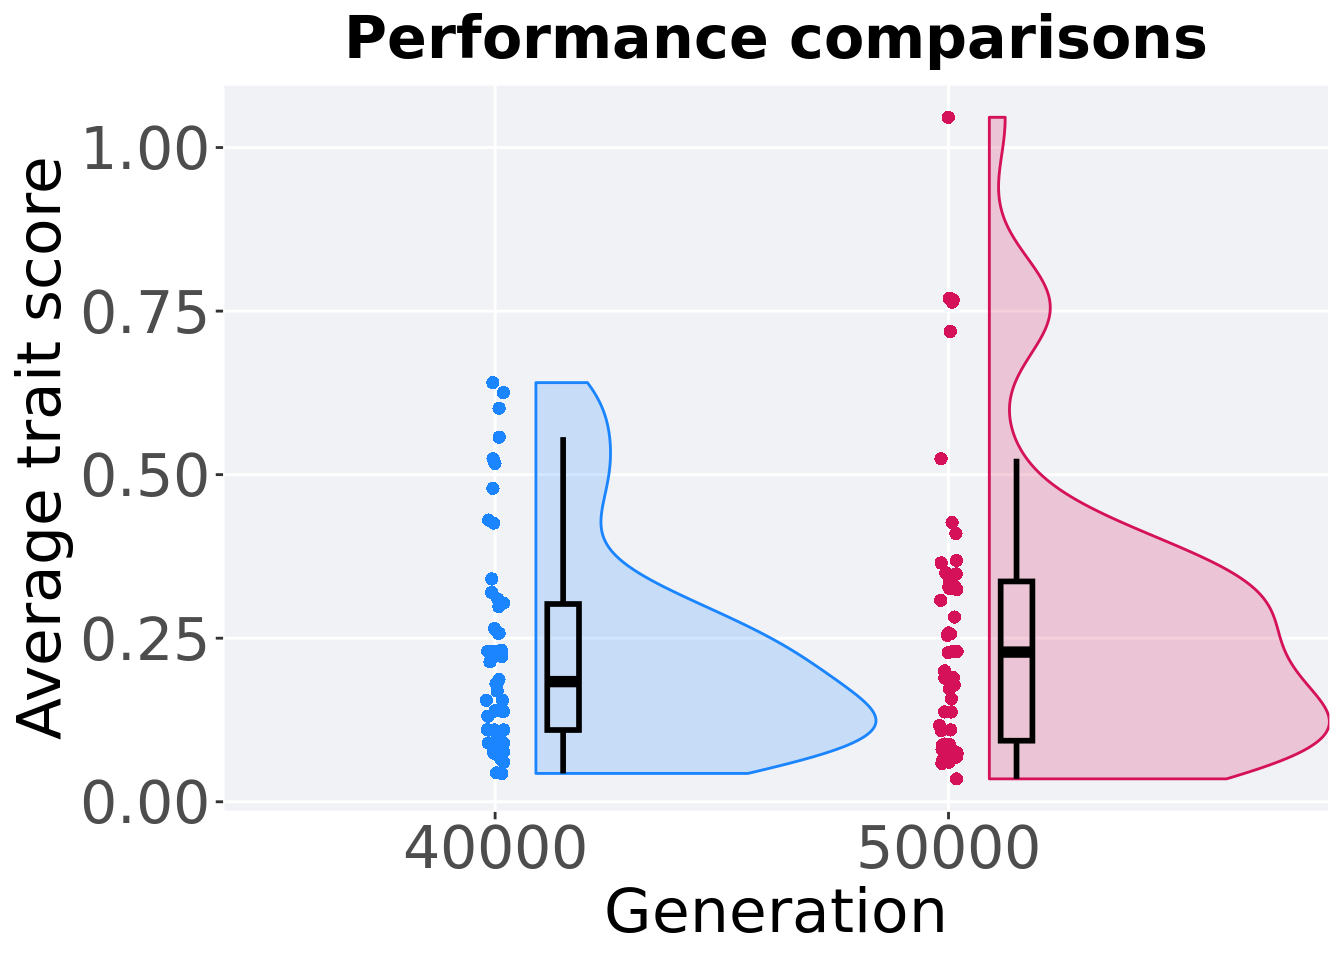
\includegraphics{mvc-diagnostics_files/figure-latex/ord-per-cmp-plt-ran-1.pdf}

Summary statistics for the best performance.

\begin{Shaded}
\begin{Highlighting}[]
\KeywordTok{filter}\NormalTok{(interval_df, acro }\OperatorTok{==}\StringTok{ 'ran'}\NormalTok{) }\OperatorTok
\StringTok{  }\KeywordTok{group_by}\NormalTok{(Generation) }\OperatorTok
\StringTok{  }\NormalTok{dplyr}\OperatorTok{::}\KeywordTok{summarise}\NormalTok{(}
    \DataTypeTok{count =} \KeywordTok{n}\NormalTok{(),}
    \DataTypeTok{na_cnt =} \KeywordTok{sum}\NormalTok{(}\KeywordTok{is.na}\NormalTok{(pop_fit_max)),}
    \DataTypeTok{min =} \KeywordTok{min}\NormalTok{(pop_fit_max }\OperatorTok{/}\StringTok{ }\NormalTok{DIMENSIONALITY, }\DataTypeTok{na.rm =} \OtherTok{TRUE}\NormalTok{),}
    \DataTypeTok{median =} \KeywordTok{median}\NormalTok{(pop_fit_max }\OperatorTok{/}\StringTok{ }\NormalTok{DIMENSIONALITY, }\DataTypeTok{na.rm =} \OtherTok{TRUE}\NormalTok{),}
    \DataTypeTok{mean =} \KeywordTok{mean}\NormalTok{(pop_fit_max }\OperatorTok{/}\StringTok{ }\NormalTok{DIMENSIONALITY, }\DataTypeTok{na.rm =} \OtherTok{TRUE}\NormalTok{),}
    \DataTypeTok{max =} \KeywordTok{max}\NormalTok{(pop_fit_max }\OperatorTok{/}\StringTok{ }\NormalTok{DIMENSIONALITY, }\DataTypeTok{na.rm =} \OtherTok{TRUE}\NormalTok{),}
    \DataTypeTok{IQR =} \KeywordTok{IQR}\NormalTok{(pop_fit_max }\OperatorTok{/}\StringTok{ }\NormalTok{DIMENSIONALITY, }\DataTypeTok{na.rm =} \OtherTok{TRUE}\NormalTok{)}
\NormalTok{  )}
\end{Highlighting}
\end{Shaded}

\begin{verbatim}
## # A tibble: 2 x 8
##   Generation count na_cnt    min median  mean   max   IQR
##   <fct>      <int>  <int>  <dbl>  <dbl> <dbl> <dbl> <dbl>
## 1 40000         50      0 0.0433  0.184 0.233 0.641 0.193
## 2 50000         50      0 0.0350  0.229 0.270 1.05  0.243
\end{verbatim}

Results for post-hoc Wilcoxon rank-sum test.

\begin{Shaded}
\begin{Highlighting}[]
\KeywordTok{wilcox.test}\NormalTok{(}\DataTypeTok{x =} \KeywordTok{filter}\NormalTok{(interval_df, acro }\OperatorTok{==}\StringTok{ 'ran'} \OperatorTok{&}\StringTok{ }\NormalTok{Generation }\OperatorTok{==}\StringTok{ }\DecValTok{50000}\NormalTok{)}\OperatorTok{$}\NormalTok{pop_fit_max,}
            \DataTypeTok{y =} \KeywordTok{filter}\NormalTok{(interval_df, acro }\OperatorTok{==}\StringTok{ 'ran'} \OperatorTok{&}\StringTok{ }\NormalTok{Generation }\OperatorTok{==}\StringTok{ }\DecValTok{40000}\NormalTok{)}\OperatorTok{$}\NormalTok{pop_fit_max,}
            \DataTypeTok{alternative =} \StringTok{'t'}\NormalTok{)}
\end{Highlighting}
\end{Shaded}

\begin{verbatim}
## 
##  Wilcoxon rank sum test with continuity correction
## 
## data:  filter(interval_df, acro == "ran" & Generation == 50000)$pop_fit_max and filter(interval_df, acro == "ran" & Generation == 40000)$pop_fit_max
## W = 1335, p-value = 0.5602
## alternative hypothesis: true location shift is not equal to 0
\end{verbatim}

\hypertarget{contradictory-objectives-results}{%
\chapter{Contradictory objectives results}\label{contradictory-objectives-results}}

Here we present the results for \textbf{activation gene coverage} and \textbf{satisfacotory trait coverage} found by each selection scheme on the contradictory objectives diagnostic with valley crossing integrated.
50 replicates are conducted for each scheme explored.

\hypertarget{analysis-dependencies-2}{%
\section{Analysis dependencies}\label{analysis-dependencies-2}}

\begin{Shaded}
\begin{Highlighting}[]
\KeywordTok{library}\NormalTok{(ggplot2)}
\KeywordTok{library}\NormalTok{(cowplot)}
\KeywordTok{library}\NormalTok{(dplyr)}
\KeywordTok{library}\NormalTok{(PupillometryR)}
\end{Highlighting}
\end{Shaded}

\hypertarget{data-setup-2}{%
\section{Data setup}\label{data-setup-2}}

\begin{Shaded}
\begin{Highlighting}[]
\NormalTok{DIR =}\StringTok{ }\KeywordTok{paste}\NormalTok{(DATA_DIR,}\StringTok{'CONTRADICTORY_OBJECTIVES/'}\NormalTok{, }\DataTypeTok{sep =} \StringTok{""}\NormalTok{, }\DataTypeTok{collapse =} \OtherTok{NULL}\NormalTok{)}
\NormalTok{over_time_df <-}\StringTok{ }\KeywordTok{read.csv}\NormalTok{(}\KeywordTok{paste}\NormalTok{(DIR,}\StringTok{'over-time.csv'}\NormalTok{, }\DataTypeTok{sep =} \StringTok{""}\NormalTok{, }\DataTypeTok{collapse =} \OtherTok{NULL}\NormalTok{), }\DataTypeTok{header =} \OtherTok{TRUE}\NormalTok{, }\DataTypeTok{stringsAsFactors =} \OtherTok{FALSE}\NormalTok{)}
\NormalTok{over_time_df}\OperatorTok{$}\NormalTok{uni_str_pos =}\StringTok{ }\NormalTok{over_time_df}\OperatorTok{$}\NormalTok{uni_str_pos }\OperatorTok{+}\StringTok{ }\NormalTok{over_time_df}\OperatorTok{$}\NormalTok{arc_acti_gene }\OperatorTok{-}\StringTok{ }\NormalTok{over_time_df}\OperatorTok{$}\NormalTok{overlap}
\NormalTok{over_time_df}\OperatorTok{$}\NormalTok{scheme <-}\StringTok{ }\KeywordTok{factor}\NormalTok{(over_time_df}\OperatorTok{$}\NormalTok{scheme, }\DataTypeTok{levels =}\NormalTok{ NAMES)}
\NormalTok{over_time_df}\OperatorTok{$}\NormalTok{acro <-}\StringTok{ }\KeywordTok{factor}\NormalTok{(over_time_df}\OperatorTok{$}\NormalTok{acro, }\DataTypeTok{levels =}\NormalTok{ ACRO)}

\NormalTok{best_df <-}\StringTok{ }\KeywordTok{read.csv}\NormalTok{(}\KeywordTok{paste}\NormalTok{(DIR,}\StringTok{'best.csv'}\NormalTok{, }\DataTypeTok{sep =} \StringTok{""}\NormalTok{, }\DataTypeTok{collapse =} \OtherTok{NULL}\NormalTok{), }\DataTypeTok{header =} \OtherTok{TRUE}\NormalTok{, }\DataTypeTok{stringsAsFactors =} \OtherTok{FALSE}\NormalTok{)}
\NormalTok{best_df}\OperatorTok{$}\NormalTok{acro <-}\StringTok{ }\KeywordTok{factor}\NormalTok{(best_df}\OperatorTok{$}\NormalTok{acro, }\DataTypeTok{levels =}\NormalTok{ ACRO)}
\end{Highlighting}
\end{Shaded}

\hypertarget{activation-gene-coverage-over-time}{%
\section{Activation gene coverage over time}\label{activation-gene-coverage-over-time}}

Activation gene coverage in a population over time.
Data points on the graph is the average activation gene coverage across 50 replicates every 2000 generations.
Shading comes from the best and worse coverage across 50 replicates.

\begin{Shaded}
\begin{Highlighting}[]
\NormalTok{lines =}\StringTok{ }\NormalTok{over_time_df }\OperatorTok
\StringTok{  }\KeywordTok{group_by}\NormalTok{(scheme, gen) }\OperatorTok
\StringTok{  }\NormalTok{dplyr}\OperatorTok{::}\KeywordTok{summarise}\NormalTok{(}
    \DataTypeTok{min =} \KeywordTok{min}\NormalTok{(uni_str_pos),}
    \DataTypeTok{mean =} \KeywordTok{mean}\NormalTok{(uni_str_pos),}
    \DataTypeTok{max =} \KeywordTok{max}\NormalTok{(uni_str_pos)}
\NormalTok{  )}
\end{Highlighting}
\end{Shaded}

\begin{verbatim}
## `summarise()` has grouped output by 'scheme'. You can override using the
## `.groups` argument.
\end{verbatim}

\begin{Shaded}
\begin{Highlighting}[]
\NormalTok{over_time_plot =}\StringTok{ }\KeywordTok{ggplot}\NormalTok{(lines, }\KeywordTok{aes}\NormalTok{(}\DataTypeTok{x=}\NormalTok{gen, }\DataTypeTok{y=}\NormalTok{mean, }\DataTypeTok{group =}\NormalTok{ scheme, }\DataTypeTok{fill =}\NormalTok{ scheme, }\DataTypeTok{color =}\NormalTok{ scheme, }\DataTypeTok{shape =}\NormalTok{ scheme)) }\OperatorTok{+}
\StringTok{  }\KeywordTok{geom_ribbon}\NormalTok{(}\KeywordTok{aes}\NormalTok{(}\DataTypeTok{ymin =}\NormalTok{ min, }\DataTypeTok{ymax =}\NormalTok{ max), }\DataTypeTok{alpha =} \FloatTok{0.1}\NormalTok{) }\OperatorTok{+}
\StringTok{  }\KeywordTok{geom_line}\NormalTok{(}\DataTypeTok{size =} \FloatTok{0.5}\NormalTok{) }\OperatorTok{+}
\StringTok{  }\KeywordTok{geom_point}\NormalTok{(}\DataTypeTok{data =} \KeywordTok{filter}\NormalTok{(lines, gen }\OperatorTok\StringTok{ }\DecValTok{2000} \OperatorTok{==}\StringTok{ }\DecValTok{0} \OperatorTok{&}\StringTok{ }\NormalTok{gen }\OperatorTok{!=}\StringTok{ }\DecValTok{0}\NormalTok{), }\DataTypeTok{size =} \FloatTok{1.5}\NormalTok{, }\DataTypeTok{stroke =} \FloatTok{2.0}\NormalTok{, }\DataTypeTok{alpha =} \FloatTok{1.0}\NormalTok{) }\OperatorTok{+}
\StringTok{  }\KeywordTok{scale_y_continuous}\NormalTok{(}
    \DataTypeTok{name=}\StringTok{"Coverage"}\NormalTok{,}
    \DataTypeTok{limits=}\KeywordTok{c}\NormalTok{(}\DecValTok{0}\NormalTok{, }\DecValTok{100}\NormalTok{),}
    \DataTypeTok{breaks=}\KeywordTok{seq}\NormalTok{(}\DecValTok{0}\NormalTok{,}\DecValTok{100}\NormalTok{, }\DecValTok{20}\NormalTok{),}
    \DataTypeTok{labels=}\KeywordTok{c}\NormalTok{(}\StringTok{"0"}\NormalTok{, }\StringTok{"20"}\NormalTok{, }\StringTok{"40"}\NormalTok{, }\StringTok{"60"}\NormalTok{, }\StringTok{"80"}\NormalTok{, }\StringTok{"100"}\NormalTok{)}
\NormalTok{  ) }\OperatorTok{+}
\StringTok{  }\KeywordTok{scale_x_continuous}\NormalTok{(}
    \DataTypeTok{name=}\StringTok{"Generations"}\NormalTok{,}
    \DataTypeTok{limits=}\KeywordTok{c}\NormalTok{(}\DecValTok{0}\NormalTok{, }\DecValTok{50000}\NormalTok{),}
    \DataTypeTok{breaks=}\KeywordTok{c}\NormalTok{(}\DecValTok{0}\NormalTok{, }\DecValTok{10000}\NormalTok{, }\DecValTok{20000}\NormalTok{, }\DecValTok{30000}\NormalTok{, }\DecValTok{40000}\NormalTok{, }\DecValTok{50000}\NormalTok{),}
    \DataTypeTok{labels=}\KeywordTok{c}\NormalTok{(}\StringTok{"0e+4"}\NormalTok{, }\StringTok{"1e+4"}\NormalTok{, }\StringTok{"2e+4"}\NormalTok{, }\StringTok{"3e+4"}\NormalTok{, }\StringTok{"4e+4"}\NormalTok{, }\StringTok{"5e+4"}\NormalTok{)}

\NormalTok{  ) }\OperatorTok{+}
\StringTok{  }\KeywordTok{scale_shape_manual}\NormalTok{(}\DataTypeTok{values=}\NormalTok{SHAPE)}\OperatorTok{+}
\StringTok{  }\KeywordTok{scale_colour_manual}\NormalTok{(}\DataTypeTok{values =}\NormalTok{ cb_palette) }\OperatorTok{+}
\StringTok{  }\KeywordTok{scale_fill_manual}\NormalTok{(}\DataTypeTok{values =}\NormalTok{ cb_palette) }\OperatorTok{+}
\StringTok{  }\KeywordTok{ggtitle}\NormalTok{(}\StringTok{'Activation gene coverage over time'}\NormalTok{)}\OperatorTok{+}
\StringTok{  }\NormalTok{p_theme }\OperatorTok{+}\StringTok{ }\KeywordTok{theme}\NormalTok{(}\DataTypeTok{legend.title=}\KeywordTok{element_blank}\NormalTok{(),}\DataTypeTok{legend.text=}\KeywordTok{element_text}\NormalTok{(}\DataTypeTok{size=}\DecValTok{12}\NormalTok{)) }\OperatorTok{+}
\StringTok{  }\KeywordTok{guides}\NormalTok{(}
    \DataTypeTok{shape=}\KeywordTok{guide_legend}\NormalTok{(}\DataTypeTok{ncol=}\DecValTok{2}\NormalTok{, }\DataTypeTok{title.position =} \StringTok{"bottom"}\NormalTok{),}
    \DataTypeTok{color=}\KeywordTok{guide_legend}\NormalTok{(}\DataTypeTok{ncol=}\DecValTok{2}\NormalTok{, }\DataTypeTok{title.position =} \StringTok{"bottom"}\NormalTok{),}
    \DataTypeTok{fill=}\KeywordTok{guide_legend}\NormalTok{(}\DataTypeTok{ncol=}\DecValTok{2}\NormalTok{, }\DataTypeTok{title.position =} \StringTok{"bottom"}\NormalTok{)}
\NormalTok{  )}

\NormalTok{over_time_plot}
\end{Highlighting}
\end{Shaded}

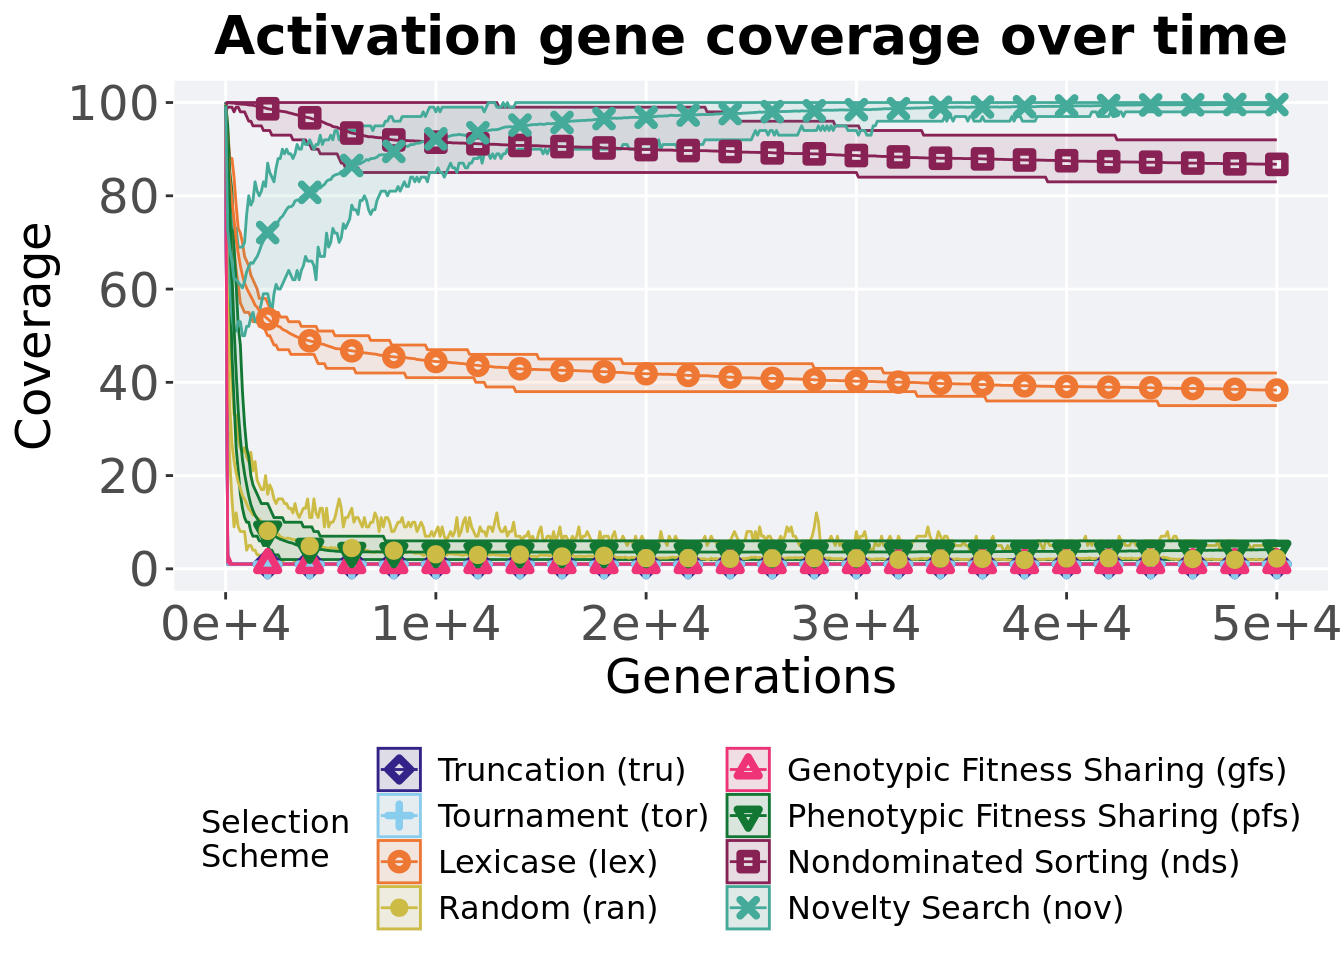
\includegraphics{mvc-diagnostics_files/figure-latex/con-act-ot-1.pdf}

\hypertarget{final-activation-gene-coverage}{%
\section{Final activation gene coverage}\label{final-activation-gene-coverage}}

Activation gene coverage found in the final population at 50,000 generations.

\begin{Shaded}
\begin{Highlighting}[]
\NormalTok{plot =}\StringTok{ }\KeywordTok{filter}\NormalTok{(over_time_df, gen }\OperatorTok{==}\StringTok{ }\DecValTok{50000}\NormalTok{) }\OperatorTok
\StringTok{  }\KeywordTok{ggplot}\NormalTok{(., }\KeywordTok{aes}\NormalTok{(}\DataTypeTok{x =}\NormalTok{ acro, }\DataTypeTok{y =}\NormalTok{ uni_str_pos, }\DataTypeTok{color =}\NormalTok{ acro, }\DataTypeTok{fill =}\NormalTok{ acro, }\DataTypeTok{shape =}\NormalTok{ acro)) }\OperatorTok{+}
\StringTok{  }\KeywordTok{geom_flat_violin}\NormalTok{(}\DataTypeTok{position =} \KeywordTok{position_nudge}\NormalTok{(}\DataTypeTok{x =} \FloatTok{.09}\NormalTok{, }\DataTypeTok{y =} \DecValTok{0}\NormalTok{), }\DataTypeTok{scale =} \StringTok{'width'}\NormalTok{, }\DataTypeTok{alpha =} \FloatTok{0.2}\NormalTok{, }\DataTypeTok{width =} \FloatTok{1.5}\NormalTok{) }\OperatorTok{+}
\StringTok{  }\KeywordTok{geom_boxplot}\NormalTok{(}\DataTypeTok{color =} \StringTok{'black'}\NormalTok{, }\DataTypeTok{width =} \FloatTok{.07}\NormalTok{, }\DataTypeTok{outlier.shape =} \OtherTok{NA}\NormalTok{, }\DataTypeTok{alpha =} \FloatTok{0.0}\NormalTok{, }\DataTypeTok{size =} \FloatTok{1.0}\NormalTok{, }\DataTypeTok{position =} \KeywordTok{position_nudge}\NormalTok{(}\DataTypeTok{x =} \FloatTok{.15}\NormalTok{, }\DataTypeTok{y =} \DecValTok{0}\NormalTok{)) }\OperatorTok{+}
\StringTok{  }\KeywordTok{geom_point}\NormalTok{(}\DataTypeTok{position =} \KeywordTok{position_jitter}\NormalTok{(}\DataTypeTok{width =} \FloatTok{0.01}\NormalTok{, }\DataTypeTok{height =} \FloatTok{0.1}\NormalTok{), }\DataTypeTok{size =} \FloatTok{2.0}\NormalTok{, }\DataTypeTok{alpha =} \FloatTok{1.0}\NormalTok{) }\OperatorTok{+}
\StringTok{  }\KeywordTok{scale_y_continuous}\NormalTok{(}
    \DataTypeTok{name=}\StringTok{"Coverage"}\NormalTok{,}
    \DataTypeTok{limits=}\KeywordTok{c}\NormalTok{(}\DecValTok{0}\NormalTok{, }\DecValTok{100}\NormalTok{),}
    \DataTypeTok{breaks=}\KeywordTok{seq}\NormalTok{(}\DecValTok{0}\NormalTok{,}\DecValTok{100}\NormalTok{, }\DecValTok{20}\NormalTok{),}
    \DataTypeTok{labels=}\KeywordTok{c}\NormalTok{(}\StringTok{"0"}\NormalTok{, }\StringTok{"20"}\NormalTok{, }\StringTok{"40"}\NormalTok{, }\StringTok{"60"}\NormalTok{, }\StringTok{"80"}\NormalTok{, }\StringTok{"100"}\NormalTok{)}
\NormalTok{  ) }\OperatorTok{+}
\StringTok{  }\KeywordTok{scale_x_discrete}\NormalTok{(}
    \DataTypeTok{name=}\StringTok{"Scheme"}
\NormalTok{  )}\OperatorTok{+}
\StringTok{  }\KeywordTok{scale_shape_manual}\NormalTok{(}\DataTypeTok{values=}\NormalTok{SHAPE)}\OperatorTok{+}
\StringTok{  }\KeywordTok{scale_colour_manual}\NormalTok{(}\DataTypeTok{values =}\NormalTok{ cb_palette, ) }\OperatorTok{+}
\StringTok{  }\KeywordTok{scale_fill_manual}\NormalTok{(}\DataTypeTok{values =}\NormalTok{ cb_palette) }\OperatorTok{+}
\StringTok{  }\KeywordTok{ggtitle}\NormalTok{(}\StringTok{'Final activation gene coverage'}\NormalTok{)}\OperatorTok{+}
\StringTok{  }\NormalTok{p_theme }\OperatorTok{+}\StringTok{ }\KeywordTok{theme}\NormalTok{(}\DataTypeTok{legend.title=}\KeywordTok{element_blank}\NormalTok{())}

\KeywordTok{plot_grid}\NormalTok{(}
\NormalTok{  plot }\OperatorTok{+}
\StringTok{    }\KeywordTok{theme}\NormalTok{(}\DataTypeTok{legend.position=}\StringTok{"none"}\NormalTok{),}
\NormalTok{  legend,}
  \DataTypeTok{nrow=}\DecValTok{2}\NormalTok{,}
  \DataTypeTok{rel_heights =} \KeywordTok{c}\NormalTok{(}\DecValTok{3}\NormalTok{,}\DecValTok{1}\NormalTok{)}
\NormalTok{)}
\end{Highlighting}
\end{Shaded}

\begin{verbatim}
## Warning: Removed 49 rows containing missing values (`geom_point()`).
\end{verbatim}

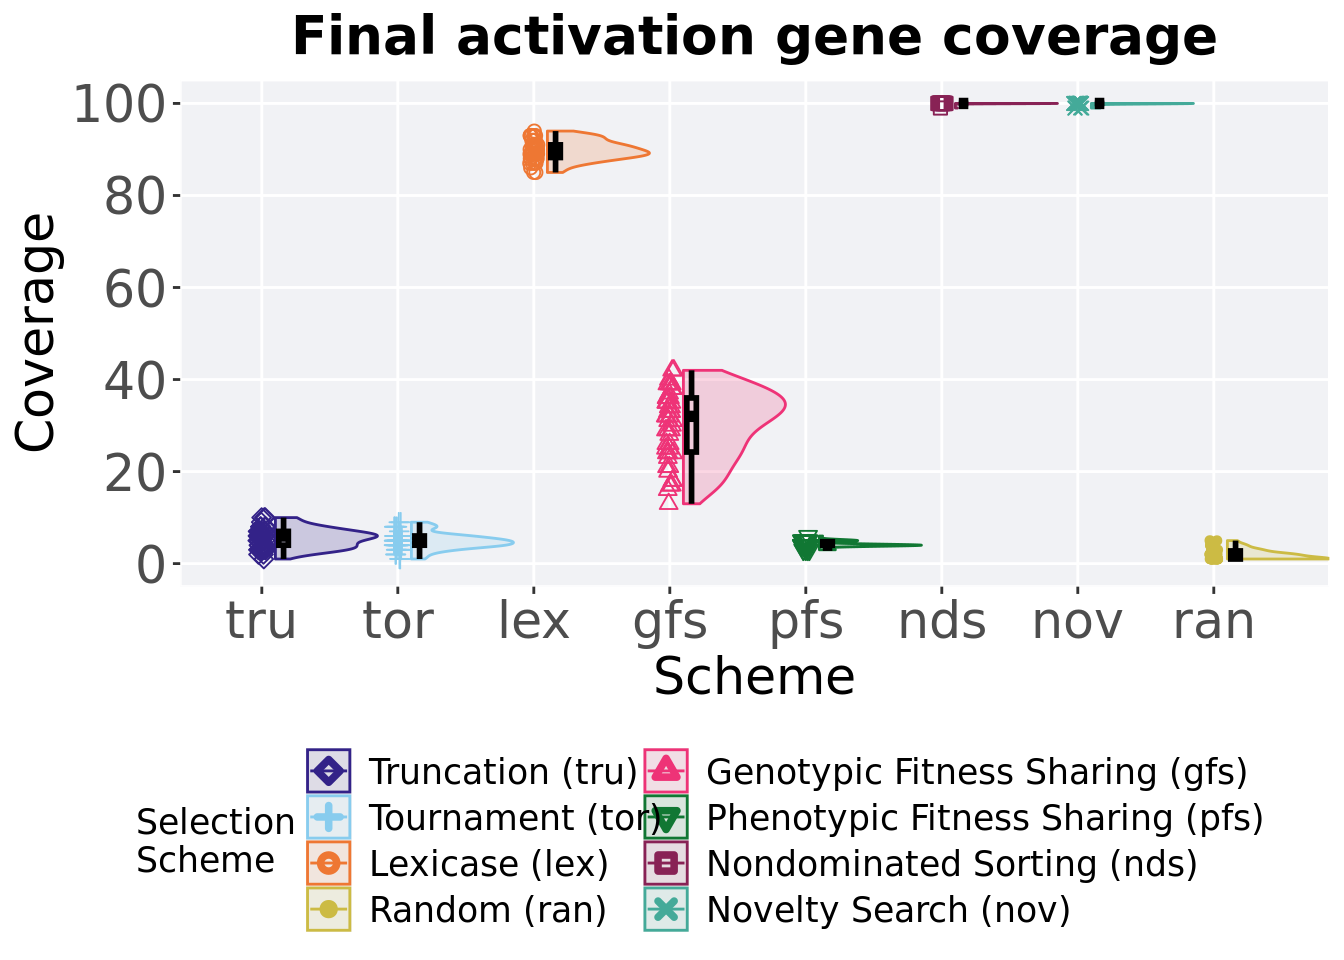
\includegraphics{mvc-diagnostics_files/figure-latex/con-act-end-1.pdf}

\hypertarget{stats-2}{%
\subsection{Stats}\label{stats-2}}

Summary statistics for the coverage found in the final population.

\begin{Shaded}
\begin{Highlighting}[]
\NormalTok{act_coverage =}\StringTok{ }\KeywordTok{filter}\NormalTok{(over_time_df, gen }\OperatorTok{==}\StringTok{ }\DecValTok{50000}\NormalTok{)}
\NormalTok{act_coverage}\OperatorTok{$}\NormalTok{acro =}\StringTok{ }\KeywordTok{factor}\NormalTok{(act_coverage}\OperatorTok{$}\NormalTok{acro, }\DataTypeTok{levels =} \KeywordTok{c}\NormalTok{(}\StringTok{'nov'}\NormalTok{,}\StringTok{'nds'}\NormalTok{,}\StringTok{'lex'}\NormalTok{,}\StringTok{'gfs'}\NormalTok{,}\StringTok{'tor'}\NormalTok{,}\StringTok{'tru'}\NormalTok{,}\StringTok{'pfs'}\NormalTok{,}\StringTok{'ran'}\NormalTok{))}
\NormalTok{act_coverage }\OperatorTok
\StringTok{  }\KeywordTok{group_by}\NormalTok{(acro) }\OperatorTok
\StringTok{  }\NormalTok{dplyr}\OperatorTok{::}\KeywordTok{summarise}\NormalTok{(}
    \DataTypeTok{count =} \KeywordTok{n}\NormalTok{(),}
    \DataTypeTok{na_cnt =} \KeywordTok{sum}\NormalTok{(}\KeywordTok{is.na}\NormalTok{(uni_str_pos)),}
    \DataTypeTok{min =} \KeywordTok{min}\NormalTok{(uni_str_pos, }\DataTypeTok{na.rm =} \OtherTok{TRUE}\NormalTok{),}
    \DataTypeTok{median =} \KeywordTok{median}\NormalTok{(uni_str_pos, }\DataTypeTok{na.rm =} \OtherTok{TRUE}\NormalTok{),}
    \DataTypeTok{mean =} \KeywordTok{mean}\NormalTok{(uni_str_pos, }\DataTypeTok{na.rm =} \OtherTok{TRUE}\NormalTok{),}
    \DataTypeTok{max =} \KeywordTok{max}\NormalTok{(uni_str_pos, }\DataTypeTok{na.rm =} \OtherTok{TRUE}\NormalTok{),}
    \DataTypeTok{IQR =} \KeywordTok{IQR}\NormalTok{(uni_str_pos, }\DataTypeTok{na.rm =} \OtherTok{TRUE}\NormalTok{)}
\NormalTok{  )}
\end{Highlighting}
\end{Shaded}

\begin{verbatim}
## # A tibble: 8 x 8
##   acro  count na_cnt   min median   mean   max   IQR
##   <fct> <int>  <int> <int>  <dbl>  <dbl> <int> <dbl>
## 1 nov      50      0    99    100  99.9    100  0   
## 2 nds      50      0    99    100 100.     100  0   
## 3 lex      50      0    83     89  89.3     94  3   
## 4 gfs      50      0     5     30  28.7     43 11.5 
## 5 tor      50      0     1      5   4.72     8  3   
## 6 tru      50      0     2      6   6.28    12  2.75
## 7 pfs      50      0     2      4   3.84     5  1   
## 8 ran      50      0     1      1   1.72     5  1
\end{verbatim}

Kruskal--Wallis test illustrates evidence of statistical differences.

\begin{Shaded}
\begin{Highlighting}[]
\KeywordTok{kruskal.test}\NormalTok{(uni_str_pos }\OperatorTok{~}\StringTok{ }\NormalTok{acro, }\DataTypeTok{data =}\NormalTok{ act_coverage)}
\end{Highlighting}
\end{Shaded}

\begin{verbatim}
## 
##  Kruskal-Wallis rank sum test
## 
## data:  uni_str_pos by acro
## Kruskal-Wallis chi-squared = 373.95, df = 7, p-value < 2.2e-16
\end{verbatim}

Results for post-hoc Wilcoxon rank-sum test with a Bonferroni correction.

\begin{Shaded}
\begin{Highlighting}[]
\KeywordTok{pairwise.wilcox.test}\NormalTok{(}\DataTypeTok{x =}\NormalTok{ act_coverage}\OperatorTok{$}\NormalTok{uni_str_pos, }\DataTypeTok{g =}\NormalTok{ act_coverage}\OperatorTok{$}\NormalTok{acro, }\DataTypeTok{p.adjust.method =} \StringTok{"bonferroni"}\NormalTok{,}
                     \DataTypeTok{paired =} \OtherTok{FALSE}\NormalTok{, }\DataTypeTok{conf.int =} \OtherTok{FALSE}\NormalTok{, }\DataTypeTok{alternative =} \StringTok{'l'}\NormalTok{)}
\end{Highlighting}
\end{Shaded}

\begin{verbatim}
## 
##  Pairwise comparisons using Wilcoxon rank sum test with continuity correction 
## 
## data:  act_coverage$uni_str_pos and act_coverage$acro 
## 
##     nov     nds     lex     gfs     tor     tru     pfs    
## nds 1.00    -       -       -       -       -       -      
## lex < 2e-16 < 2e-16 -       -       -       -       -      
## gfs < 2e-16 < 2e-16 < 2e-16 -       -       -       -      
## tor < 2e-16 < 2e-16 < 2e-16 1.3e-15 -       -       -      
## tru < 2e-16 < 2e-16 < 2e-16 7.3e-15 1.00    -       -      
## pfs < 2e-16 < 2e-16 < 2e-16 < 2e-16 0.05    3.4e-10 -      
## ran < 2e-16 < 2e-16 < 2e-16 < 2e-16 1.4e-12 1.9e-15 1.8e-12
## 
## P value adjustment method: bonferroni
\end{verbatim}

\hypertarget{satisfactory-trait-coverage-over-time}{%
\section{Satisfactory trait coverage over time}\label{satisfactory-trait-coverage-over-time}}

Satisfactory trait coverage in a population over time.
Data points on the graph is the average activation gene coverage across 50 replicates every 2000 generations.
Shading comes from the best and worse coverage across 50 replicates.

\begin{Shaded}
\begin{Highlighting}[]
\NormalTok{lines =}\StringTok{ }\NormalTok{over_time_df }\OperatorTok
\StringTok{  }\KeywordTok{group_by}\NormalTok{(scheme, gen) }\OperatorTok
\StringTok{  }\NormalTok{dplyr}\OperatorTok{::}\KeywordTok{summarise}\NormalTok{(}
    \DataTypeTok{min =} \KeywordTok{min}\NormalTok{(pop_uni_obj),}
    \DataTypeTok{mean =} \KeywordTok{mean}\NormalTok{(pop_uni_obj),}
    \DataTypeTok{max =} \KeywordTok{max}\NormalTok{(pop_uni_obj)}
\NormalTok{  )}
\end{Highlighting}
\end{Shaded}

\begin{verbatim}
## `summarise()` has grouped output by 'scheme'. You can override using the
## `.groups` argument.
\end{verbatim}

\begin{Shaded}
\begin{Highlighting}[]
\NormalTok{over_time_plot =}\StringTok{ }\KeywordTok{ggplot}\NormalTok{(lines, }\KeywordTok{aes}\NormalTok{(}\DataTypeTok{x=}\NormalTok{gen, }\DataTypeTok{y=}\NormalTok{mean, }\DataTypeTok{group =}\NormalTok{ scheme, }\DataTypeTok{fill =}\NormalTok{ scheme, }\DataTypeTok{color =}\NormalTok{ scheme, }\DataTypeTok{shape =}\NormalTok{ scheme)) }\OperatorTok{+}
\StringTok{  }\KeywordTok{geom_ribbon}\NormalTok{(}\KeywordTok{aes}\NormalTok{(}\DataTypeTok{ymin =}\NormalTok{ min, }\DataTypeTok{ymax =}\NormalTok{ max), }\DataTypeTok{alpha =} \FloatTok{0.1}\NormalTok{) }\OperatorTok{+}
\StringTok{  }\KeywordTok{geom_line}\NormalTok{(}\DataTypeTok{size =} \FloatTok{0.5}\NormalTok{) }\OperatorTok{+}
\StringTok{  }\KeywordTok{geom_point}\NormalTok{(}\DataTypeTok{data =} \KeywordTok{filter}\NormalTok{(lines, gen }\OperatorTok\StringTok{ }\DecValTok{2000} \OperatorTok{==}\StringTok{ }\DecValTok{0} \OperatorTok{&}\StringTok{ }\NormalTok{gen }\OperatorTok{!=}\StringTok{ }\DecValTok{0}\NormalTok{), }\DataTypeTok{size =} \FloatTok{1.5}\NormalTok{, }\DataTypeTok{stroke =} \FloatTok{2.0}\NormalTok{, }\DataTypeTok{alpha =} \FloatTok{1.0}\NormalTok{) }\OperatorTok{+}
\StringTok{  }\KeywordTok{scale_y_continuous}\NormalTok{(}
    \DataTypeTok{name=}\StringTok{"Coverage"}
\NormalTok{  ) }\OperatorTok{+}
\StringTok{  }\KeywordTok{scale_x_continuous}\NormalTok{(}
    \DataTypeTok{name=}\StringTok{"Generations"}\NormalTok{,}
    \DataTypeTok{limits=}\KeywordTok{c}\NormalTok{(}\DecValTok{0}\NormalTok{, }\DecValTok{50000}\NormalTok{),}
    \DataTypeTok{breaks=}\KeywordTok{c}\NormalTok{(}\DecValTok{0}\NormalTok{, }\DecValTok{10000}\NormalTok{, }\DecValTok{20000}\NormalTok{, }\DecValTok{30000}\NormalTok{, }\DecValTok{40000}\NormalTok{, }\DecValTok{50000}\NormalTok{),}
    \DataTypeTok{labels=}\KeywordTok{c}\NormalTok{(}\StringTok{"0e+4"}\NormalTok{, }\StringTok{"1e+4"}\NormalTok{, }\StringTok{"2e+4"}\NormalTok{, }\StringTok{"3e+4"}\NormalTok{, }\StringTok{"4e+4"}\NormalTok{, }\StringTok{"5e+4"}\NormalTok{)}

\NormalTok{  ) }\OperatorTok{+}
\StringTok{  }\KeywordTok{scale_shape_manual}\NormalTok{(}\DataTypeTok{values=}\NormalTok{SHAPE)}\OperatorTok{+}
\StringTok{  }\KeywordTok{scale_colour_manual}\NormalTok{(}\DataTypeTok{values =}\NormalTok{ cb_palette) }\OperatorTok{+}
\StringTok{  }\KeywordTok{scale_fill_manual}\NormalTok{(}\DataTypeTok{values =}\NormalTok{ cb_palette) }\OperatorTok{+}
\StringTok{  }\KeywordTok{ggtitle}\NormalTok{(}\StringTok{'Satisfactory trait coverage over time'}\NormalTok{)}\OperatorTok{+}
\StringTok{  }\NormalTok{p_theme }\OperatorTok{+}\StringTok{ }\KeywordTok{theme}\NormalTok{(}\DataTypeTok{legend.title=}\KeywordTok{element_blank}\NormalTok{(),}\DataTypeTok{legend.text=}\KeywordTok{element_text}\NormalTok{(}\DataTypeTok{size=}\DecValTok{12}\NormalTok{)) }\OperatorTok{+}
\StringTok{  }\KeywordTok{guides}\NormalTok{(}
    \DataTypeTok{shape=}\KeywordTok{guide_legend}\NormalTok{(}\DataTypeTok{ncol=}\DecValTok{2}\NormalTok{, }\DataTypeTok{title.position =} \StringTok{"bottom"}\NormalTok{),}
    \DataTypeTok{color=}\KeywordTok{guide_legend}\NormalTok{(}\DataTypeTok{ncol=}\DecValTok{2}\NormalTok{, }\DataTypeTok{title.position =} \StringTok{"bottom"}\NormalTok{),}
    \DataTypeTok{fill=}\KeywordTok{guide_legend}\NormalTok{(}\DataTypeTok{ncol=}\DecValTok{2}\NormalTok{, }\DataTypeTok{title.position =} \StringTok{"bottom"}\NormalTok{)}
\NormalTok{  )}

\NormalTok{over_time_plot}
\end{Highlighting}
\end{Shaded}

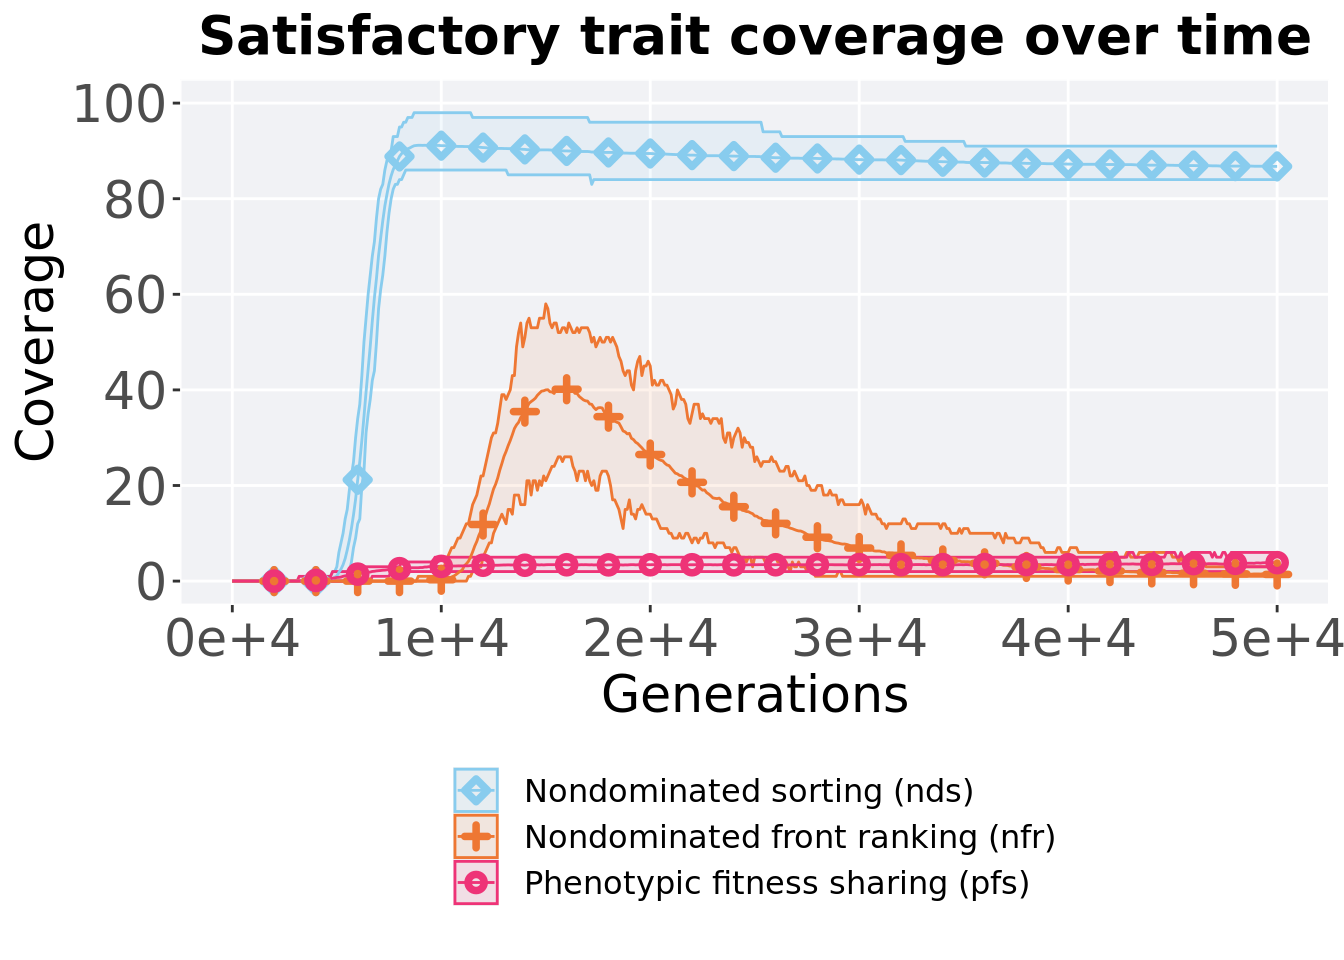
\includegraphics{mvc-diagnostics_files/figure-latex/con-sat-ot-1.pdf}

\hypertarget{best-satisfactory-trait-coverage-throughout}{%
\section{Best satisfactory trait coverage throughout}\label{best-satisfactory-trait-coverage-throughout}}

Best satisfactory trait coverage reached throughout 50,000 generations in a population.

\begin{Shaded}
\begin{Highlighting}[]
\NormalTok{plot =}\StringTok{ }\KeywordTok{filter}\NormalTok{(best_df, var }\OperatorTok{==}\StringTok{ 'pop_uni_obj'}\NormalTok{) }\OperatorTok
\StringTok{  }\KeywordTok{ggplot}\NormalTok{(., }\KeywordTok{aes}\NormalTok{(}\DataTypeTok{x =}\NormalTok{ acro, }\DataTypeTok{y =}\NormalTok{ val, }\DataTypeTok{color =}\NormalTok{ acro, }\DataTypeTok{fill =}\NormalTok{ acro, }\DataTypeTok{shape =}\NormalTok{ acro)) }\OperatorTok{+}
\StringTok{  }\KeywordTok{geom_flat_violin}\NormalTok{(}\DataTypeTok{position =} \KeywordTok{position_nudge}\NormalTok{(}\DataTypeTok{x =} \FloatTok{.09}\NormalTok{, }\DataTypeTok{y =} \DecValTok{0}\NormalTok{), }\DataTypeTok{scale =} \StringTok{'width'}\NormalTok{, }\DataTypeTok{alpha =} \FloatTok{0.2}\NormalTok{, }\DataTypeTok{width =} \FloatTok{1.5}\NormalTok{) }\OperatorTok{+}
\StringTok{  }\KeywordTok{geom_boxplot}\NormalTok{(}\DataTypeTok{color =} \StringTok{'black'}\NormalTok{, }\DataTypeTok{width =} \FloatTok{.07}\NormalTok{, }\DataTypeTok{outlier.shape =} \OtherTok{NA}\NormalTok{, }\DataTypeTok{alpha =} \FloatTok{0.0}\NormalTok{, }\DataTypeTok{size =} \FloatTok{1.0}\NormalTok{, }\DataTypeTok{position =} \KeywordTok{position_nudge}\NormalTok{(}\DataTypeTok{x =} \FloatTok{.15}\NormalTok{, }\DataTypeTok{y =} \DecValTok{0}\NormalTok{)) }\OperatorTok{+}
\StringTok{  }\KeywordTok{geom_point}\NormalTok{(}\DataTypeTok{position =} \KeywordTok{position_jitter}\NormalTok{(}\DataTypeTok{width =} \FloatTok{0.01}\NormalTok{, }\DataTypeTok{height =} \FloatTok{0.1}\NormalTok{), }\DataTypeTok{size =} \FloatTok{2.0}\NormalTok{, }\DataTypeTok{alpha =} \FloatTok{1.0}\NormalTok{) }\OperatorTok{+}
\StringTok{  }\KeywordTok{scale_y_continuous}\NormalTok{(}
    \DataTypeTok{name=}\StringTok{"Coverage"}\NormalTok{,}
    \DataTypeTok{limits=}\KeywordTok{c}\NormalTok{(}\DecValTok{0}\NormalTok{, }\DecValTok{5}\NormalTok{)}
\NormalTok{  ) }\OperatorTok{+}
\StringTok{  }\KeywordTok{scale_x_discrete}\NormalTok{(}
    \DataTypeTok{name=}\StringTok{"Scheme"}
\NormalTok{  )}\OperatorTok{+}
\StringTok{  }\KeywordTok{scale_shape_manual}\NormalTok{(}\DataTypeTok{values=}\NormalTok{SHAPE)}\OperatorTok{+}
\StringTok{  }\KeywordTok{scale_colour_manual}\NormalTok{(}\DataTypeTok{values =}\NormalTok{ cb_palette, ) }\OperatorTok{+}
\StringTok{  }\KeywordTok{scale_fill_manual}\NormalTok{(}\DataTypeTok{values =}\NormalTok{ cb_palette) }\OperatorTok{+}
\StringTok{  }\KeywordTok{ggtitle}\NormalTok{(}\StringTok{'Best satisfactory trait coverage'}\NormalTok{)}\OperatorTok{+}
\StringTok{  }\NormalTok{p_theme }\OperatorTok{+}\StringTok{ }\KeywordTok{theme}\NormalTok{(}\DataTypeTok{legend.title=}\KeywordTok{element_blank}\NormalTok{())}

\KeywordTok{plot_grid}\NormalTok{(}
\NormalTok{  plot }\OperatorTok{+}
\StringTok{    }\KeywordTok{theme}\NormalTok{(}\DataTypeTok{legend.position=}\StringTok{"none"}\NormalTok{),}
\NormalTok{  legend,}
  \DataTypeTok{nrow=}\DecValTok{2}\NormalTok{,}
  \DataTypeTok{rel_heights =} \KeywordTok{c}\NormalTok{(}\DecValTok{3}\NormalTok{,}\DecValTok{1}\NormalTok{)}
\NormalTok{)}
\end{Highlighting}
\end{Shaded}

\begin{verbatim}
## Warning: Removed 189 rows containing missing values (`geom_point()`).
\end{verbatim}

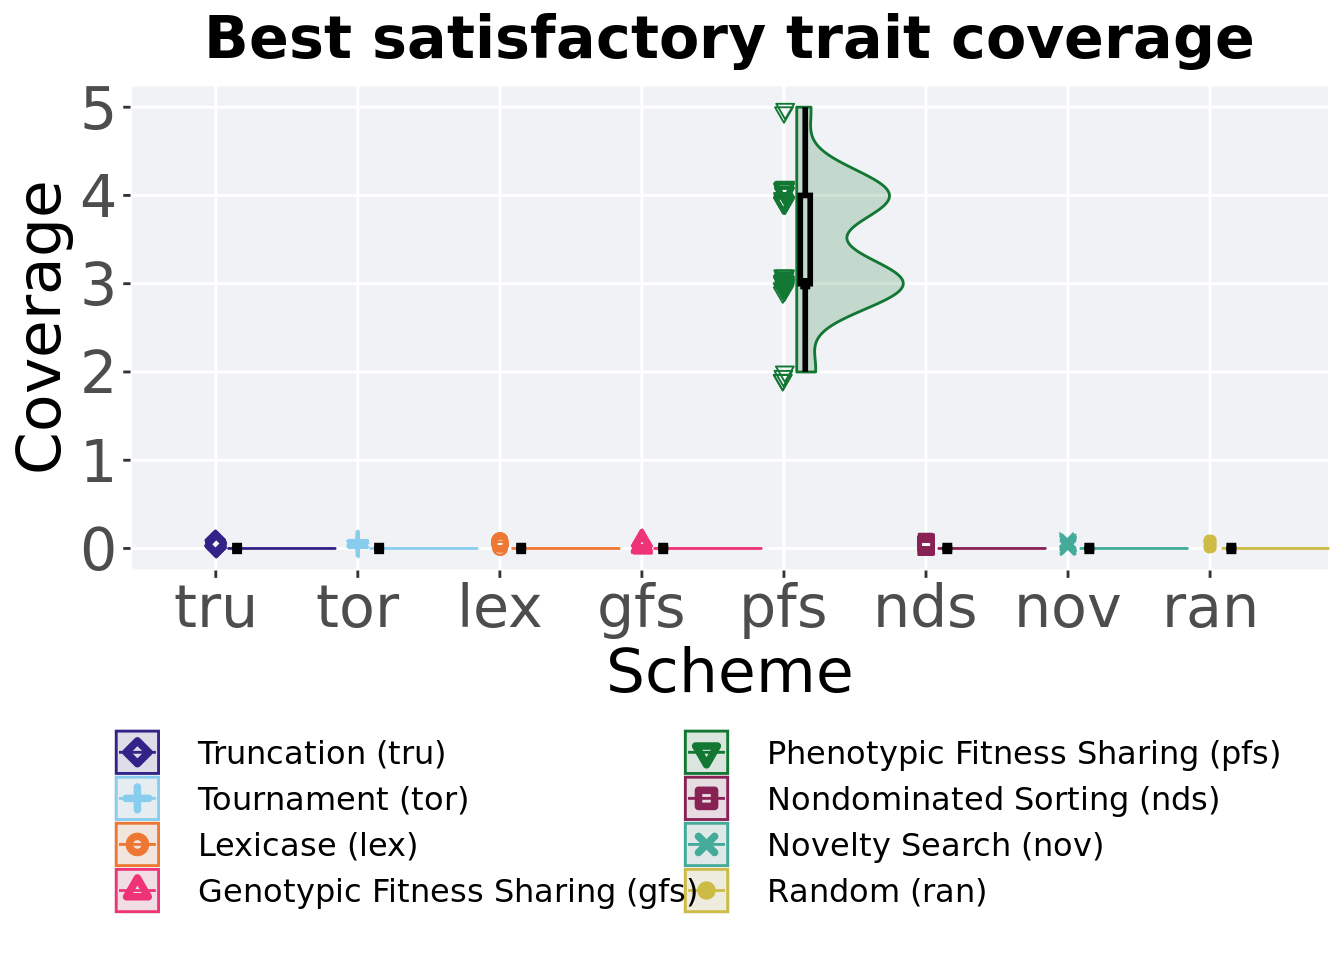
\includegraphics{mvc-diagnostics_files/figure-latex/con-sat-bst-1.pdf}

\hypertarget{stats-3}{%
\subsection{Stats}\label{stats-3}}

Summary statistics for the best coverage.

\begin{Shaded}
\begin{Highlighting}[]
\NormalTok{sat_coverage =}\StringTok{ }\KeywordTok{filter}\NormalTok{(best_df, var }\OperatorTok{==}\StringTok{ 'pop_uni_obj'}\NormalTok{)}
\NormalTok{sat_coverage}\OperatorTok{$}\NormalTok{acro =}\StringTok{ }\KeywordTok{factor}\NormalTok{(sat_coverage}\OperatorTok{$}\NormalTok{acro, }\DataTypeTok{levels =} \KeywordTok{c}\NormalTok{(}\StringTok{'pfs'}\NormalTok{,}\StringTok{'nds'}\NormalTok{,}\StringTok{'lex'}\NormalTok{,}\StringTok{'gfs'}\NormalTok{,}\StringTok{'tor'}\NormalTok{,}\StringTok{'tru'}\NormalTok{,}\StringTok{'nov'}\NormalTok{,}\StringTok{'ran'}\NormalTok{))}
\NormalTok{sat_coverage }\OperatorTok
\StringTok{  }\KeywordTok{group_by}\NormalTok{(acro) }\OperatorTok
\StringTok{  }\NormalTok{dplyr}\OperatorTok{::}\KeywordTok{summarise}\NormalTok{(}
    \DataTypeTok{count =} \KeywordTok{n}\NormalTok{(),}
    \DataTypeTok{na_cnt =} \KeywordTok{sum}\NormalTok{(}\KeywordTok{is.na}\NormalTok{(val)),}
    \DataTypeTok{min =} \KeywordTok{min}\NormalTok{(val, }\DataTypeTok{na.rm =} \OtherTok{TRUE}\NormalTok{),}
    \DataTypeTok{median =} \KeywordTok{median}\NormalTok{(val, }\DataTypeTok{na.rm =} \OtherTok{TRUE}\NormalTok{),}
    \DataTypeTok{mean =} \KeywordTok{mean}\NormalTok{(val, }\DataTypeTok{na.rm =} \OtherTok{TRUE}\NormalTok{),}
    \DataTypeTok{max =} \KeywordTok{max}\NormalTok{(val, }\DataTypeTok{na.rm =} \OtherTok{TRUE}\NormalTok{),}
    \DataTypeTok{IQR =} \KeywordTok{IQR}\NormalTok{(val, }\DataTypeTok{na.rm =} \OtherTok{TRUE}\NormalTok{)}
\NormalTok{  )}
\end{Highlighting}
\end{Shaded}

\begin{verbatim}
## # A tibble: 8 x 8
##   acro  count na_cnt   min median  mean   max   IQR
##   <fct> <int>  <int> <dbl>  <dbl> <dbl> <dbl> <dbl>
## 1 pfs      50      0     2      3  3.44     5     1
## 2 nds      50      0     0      0  0        0     0
## 3 lex      50      0     0      0  0        0     0
## 4 gfs      50      0     0      0  0        0     0
## 5 tor      50      0     0      0  0        0     0
## 6 tru      50      0     0      0  0        0     0
## 7 nov      50      0     0      0  0        0     0
## 8 ran      50      0     0      0  0        0     0
\end{verbatim}

Kruskal--Wallis test illustrates evidence of statistical differences.

\begin{Shaded}
\begin{Highlighting}[]
\KeywordTok{kruskal.test}\NormalTok{(val }\OperatorTok{~}\StringTok{ }\NormalTok{acro, }\DataTypeTok{data =}\NormalTok{ sat_coverage)}
\end{Highlighting}
\end{Shaded}

\begin{verbatim}
## 
##  Kruskal-Wallis rank sum test
## 
## data:  val by acro
## Kruskal-Wallis chi-squared = 397.02, df = 7, p-value < 2.2e-16
\end{verbatim}

Results for post-hoc Wilcoxon rank-sum test with a Bonferroni correction.

\begin{Shaded}
\begin{Highlighting}[]
\KeywordTok{pairwise.wilcox.test}\NormalTok{(}\DataTypeTok{x =}\NormalTok{ sat_coverage}\OperatorTok{$}\NormalTok{val, }\DataTypeTok{g =}\NormalTok{ sat_coverage}\OperatorTok{$}\NormalTok{acro, }\DataTypeTok{p.adjust.method =} \StringTok{"bonferroni"}\NormalTok{,}
                     \DataTypeTok{paired =} \OtherTok{FALSE}\NormalTok{, }\DataTypeTok{conf.int =} \OtherTok{FALSE}\NormalTok{, }\DataTypeTok{alternative =} \StringTok{'l'}\NormalTok{)}
\end{Highlighting}
\end{Shaded}

\begin{verbatim}
## 
##  Pairwise comparisons using Wilcoxon rank sum test with continuity correction 
## 
## data:  sat_coverage$val and sat_coverage$acro 
## 
##     pfs    nds lex gfs tor tru nov
## nds <2e-16 -   -   -   -   -   -  
## lex <2e-16 1   -   -   -   -   -  
## gfs <2e-16 1   1   -   -   -   -  
## tor <2e-16 1   1   1   -   -   -  
## tru <2e-16 1   1   1   1   -   -  
## nov <2e-16 1   1   1   1   1   -  
## ran <2e-16 1   1   1   1   1   1  
## 
## P value adjustment method: bonferroni
\end{verbatim}

\hypertarget{final-satisfactory-trait-coverage}{%
\section{Final satisfactory trait coverage}\label{final-satisfactory-trait-coverage}}

Satisfactory trait coverage found in the final population at 50,000 generations.

\begin{Shaded}
\begin{Highlighting}[]
\NormalTok{plot =}\StringTok{ }\KeywordTok{filter}\NormalTok{(over_time_df, gen }\OperatorTok{==}\StringTok{ }\DecValTok{50000}\NormalTok{) }\OperatorTok
\StringTok{  }\KeywordTok{ggplot}\NormalTok{(., }\KeywordTok{aes}\NormalTok{(}\DataTypeTok{x =}\NormalTok{ acro, }\DataTypeTok{y =}\NormalTok{ pop_uni_obj, }\DataTypeTok{color =}\NormalTok{ acro, }\DataTypeTok{fill =}\NormalTok{ acro, }\DataTypeTok{shape =}\NormalTok{ acro)) }\OperatorTok{+}
\StringTok{  }\KeywordTok{geom_flat_violin}\NormalTok{(}\DataTypeTok{position =} \KeywordTok{position_nudge}\NormalTok{(}\DataTypeTok{x =} \FloatTok{.09}\NormalTok{, }\DataTypeTok{y =} \DecValTok{0}\NormalTok{), }\DataTypeTok{scale =} \StringTok{'width'}\NormalTok{, }\DataTypeTok{alpha =} \FloatTok{0.2}\NormalTok{, }\DataTypeTok{width =} \FloatTok{1.5}\NormalTok{) }\OperatorTok{+}
\StringTok{  }\KeywordTok{geom_boxplot}\NormalTok{(}\DataTypeTok{color =} \StringTok{'black'}\NormalTok{, }\DataTypeTok{width =} \FloatTok{.07}\NormalTok{, }\DataTypeTok{outlier.shape =} \OtherTok{NA}\NormalTok{, }\DataTypeTok{alpha =} \FloatTok{0.0}\NormalTok{, }\DataTypeTok{size =} \FloatTok{1.0}\NormalTok{, }\DataTypeTok{position =} \KeywordTok{position_nudge}\NormalTok{(}\DataTypeTok{x =} \FloatTok{.15}\NormalTok{, }\DataTypeTok{y =} \DecValTok{0}\NormalTok{)) }\OperatorTok{+}
\StringTok{  }\KeywordTok{geom_point}\NormalTok{(}\DataTypeTok{position =} \KeywordTok{position_jitter}\NormalTok{(}\DataTypeTok{width =} \FloatTok{0.01}\NormalTok{, }\DataTypeTok{height =} \FloatTok{0.1}\NormalTok{), }\DataTypeTok{size =} \FloatTok{2.0}\NormalTok{, }\DataTypeTok{alpha =} \FloatTok{1.0}\NormalTok{) }\OperatorTok{+}
\StringTok{  }\KeywordTok{scale_y_continuous}\NormalTok{(}
    \DataTypeTok{name=}\StringTok{"Coverage"}\NormalTok{,}
    \DataTypeTok{limits=}\KeywordTok{c}\NormalTok{(}\DecValTok{0}\NormalTok{, }\DecValTok{5}\NormalTok{)}
\NormalTok{  ) }\OperatorTok{+}
\StringTok{  }\KeywordTok{scale_x_discrete}\NormalTok{(}
    \DataTypeTok{name=}\StringTok{"Scheme"}
\NormalTok{  )}\OperatorTok{+}
\StringTok{  }\KeywordTok{scale_shape_manual}\NormalTok{(}\DataTypeTok{values=}\NormalTok{SHAPE)}\OperatorTok{+}
\StringTok{  }\KeywordTok{scale_colour_manual}\NormalTok{(}\DataTypeTok{values =}\NormalTok{ cb_palette, ) }\OperatorTok{+}
\StringTok{  }\KeywordTok{scale_fill_manual}\NormalTok{(}\DataTypeTok{values =}\NormalTok{ cb_palette) }\OperatorTok{+}
\StringTok{  }\KeywordTok{ggtitle}\NormalTok{(}\StringTok{'Final satisfactory trait coverage'}\NormalTok{)}\OperatorTok{+}
\StringTok{  }\NormalTok{p_theme }\OperatorTok{+}\StringTok{ }\KeywordTok{theme}\NormalTok{(}\DataTypeTok{legend.title=}\KeywordTok{element_blank}\NormalTok{())}

\KeywordTok{plot_grid}\NormalTok{(}
\NormalTok{  plot }\OperatorTok{+}
\StringTok{    }\KeywordTok{theme}\NormalTok{(}\DataTypeTok{legend.position=}\StringTok{"none"}\NormalTok{),}
\NormalTok{  legend,}
  \DataTypeTok{nrow=}\DecValTok{2}\NormalTok{,}
  \DataTypeTok{rel_heights =} \KeywordTok{c}\NormalTok{(}\DecValTok{3}\NormalTok{,}\DecValTok{1}\NormalTok{)}
\NormalTok{)}
\end{Highlighting}
\end{Shaded}

\begin{verbatim}
## Warning: Removed 173 rows containing missing values (`geom_point()`).
\end{verbatim}

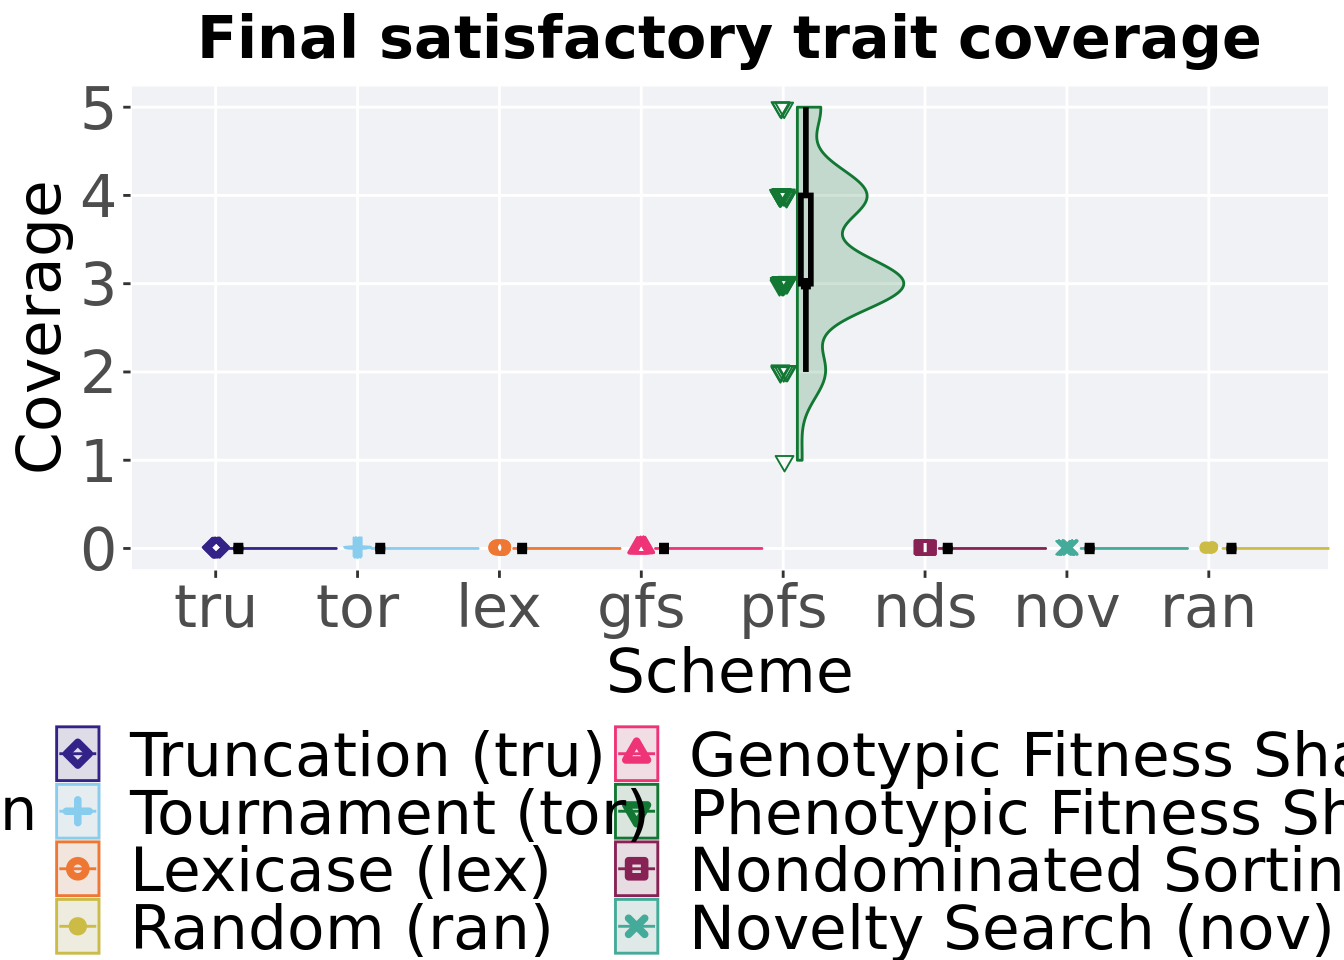
\includegraphics{mvc-diagnostics_files/figure-latex/con-sat-end-1.pdf}

\hypertarget{stats-4}{%
\subsection{Stats}\label{stats-4}}

Summary statistics for the coverage found in the final population.

\begin{Shaded}
\begin{Highlighting}[]
\NormalTok{act_coverage =}\StringTok{ }\KeywordTok{filter}\NormalTok{(over_time_df, gen }\OperatorTok{==}\StringTok{ }\DecValTok{50000}\NormalTok{)}
\NormalTok{act_coverage}\OperatorTok{$}\NormalTok{acro =}\StringTok{ }\KeywordTok{factor}\NormalTok{(act_coverage}\OperatorTok{$}\NormalTok{acro, }\DataTypeTok{levels =} \KeywordTok{c}\NormalTok{(}\StringTok{'pfs'}\NormalTok{,}\StringTok{'nds'}\NormalTok{,}\StringTok{'lex'}\NormalTok{,}\StringTok{'gfs'}\NormalTok{,}\StringTok{'tor'}\NormalTok{,}\StringTok{'tru'}\NormalTok{,}\StringTok{'nov'}\NormalTok{,}\StringTok{'ran'}\NormalTok{))}
\NormalTok{act_coverage }\OperatorTok
\StringTok{  }\KeywordTok{group_by}\NormalTok{(acro) }\OperatorTok
\StringTok{  }\NormalTok{dplyr}\OperatorTok{::}\KeywordTok{summarise}\NormalTok{(}
    \DataTypeTok{count =} \KeywordTok{n}\NormalTok{(),}
    \DataTypeTok{na_cnt =} \KeywordTok{sum}\NormalTok{(}\KeywordTok{is.na}\NormalTok{(pop_uni_obj)),}
    \DataTypeTok{min =} \KeywordTok{min}\NormalTok{(pop_uni_obj, }\DataTypeTok{na.rm =} \OtherTok{TRUE}\NormalTok{),}
    \DataTypeTok{median =} \KeywordTok{median}\NormalTok{(pop_uni_obj, }\DataTypeTok{na.rm =} \OtherTok{TRUE}\NormalTok{),}
    \DataTypeTok{mean =} \KeywordTok{mean}\NormalTok{(pop_uni_obj, }\DataTypeTok{na.rm =} \OtherTok{TRUE}\NormalTok{),}
    \DataTypeTok{max =} \KeywordTok{max}\NormalTok{(pop_uni_obj, }\DataTypeTok{na.rm =} \OtherTok{TRUE}\NormalTok{),}
    \DataTypeTok{IQR =} \KeywordTok{IQR}\NormalTok{(pop_uni_obj, }\DataTypeTok{na.rm =} \OtherTok{TRUE}\NormalTok{)}
\NormalTok{  )}
\end{Highlighting}
\end{Shaded}

\begin{verbatim}
## # A tibble: 8 x 8
##   acro  count na_cnt   min median  mean   max   IQR
##   <fct> <int>  <int> <int>  <dbl> <dbl> <int> <dbl>
## 1 pfs      50      0     2      3  3.32     5     1
## 2 nds      50      0     0      0  0        0     0
## 3 lex      50      0     0      0  0        0     0
## 4 gfs      50      0     0      0  0        0     0
## 5 tor      50      0     0      0  0        0     0
## 6 tru      50      0     0      0  0        0     0
## 7 nov      50      0     0      0  0        0     0
## 8 ran      50      0     0      0  0        0     0
\end{verbatim}

Kruskal--Wallis test illustrates evidence of statistical differences.

\begin{Shaded}
\begin{Highlighting}[]
\KeywordTok{kruskal.test}\NormalTok{(pop_uni_obj }\OperatorTok{~}\StringTok{ }\NormalTok{acro, }\DataTypeTok{data =}\NormalTok{ act_coverage)}
\end{Highlighting}
\end{Shaded}

\begin{verbatim}
## 
##  Kruskal-Wallis rank sum test
## 
## data:  pop_uni_obj by acro
## Kruskal-Wallis chi-squared = 396.97, df = 7, p-value < 2.2e-16
\end{verbatim}

Results for post-hoc Wilcoxon rank-sum test with a Bonferroni correction.

\begin{Shaded}
\begin{Highlighting}[]
\KeywordTok{pairwise.wilcox.test}\NormalTok{(}\DataTypeTok{x =}\NormalTok{ act_coverage}\OperatorTok{$}\NormalTok{pop_uni_obj, }\DataTypeTok{g =}\NormalTok{ act_coverage}\OperatorTok{$}\NormalTok{acro, }\DataTypeTok{p.adjust.method =} \StringTok{"bonferroni"}\NormalTok{,}
                     \DataTypeTok{paired =} \OtherTok{FALSE}\NormalTok{, }\DataTypeTok{conf.int =} \OtherTok{FALSE}\NormalTok{, }\DataTypeTok{alternative =} \StringTok{'l'}\NormalTok{)}
\end{Highlighting}
\end{Shaded}

\begin{verbatim}
## 
##  Pairwise comparisons using Wilcoxon rank sum test with continuity correction 
## 
## data:  act_coverage$pop_uni_obj and act_coverage$acro 
## 
##     pfs    nds lex gfs tor tru nov
## nds <2e-16 -   -   -   -   -   -  
## lex <2e-16 1   -   -   -   -   -  
## gfs <2e-16 1   1   -   -   -   -  
## tor <2e-16 1   1   1   -   -   -  
## tru <2e-16 1   1   1   1   -   -  
## nov <2e-16 1   1   1   1   1   -  
## ran <2e-16 1   1   1   1   1   1  
## 
## P value adjustment method: bonferroni
\end{verbatim}

\hypertarget{best-trait-value-over-time}{%
\section{Best trait value over time}\label{best-trait-value-over-time}}

Best trait value in a population over time.
Data points on the graph is the average trait value across 50 replicates every 2000 generations.
Shading comes from the best and worse trait value across 50 replicates.

\begin{Shaded}
\begin{Highlighting}[]
\NormalTok{lines =}\StringTok{ }\NormalTok{over_time_df }\OperatorTok
\StringTok{  }\KeywordTok{group_by}\NormalTok{(scheme, gen) }\OperatorTok
\StringTok{  }\NormalTok{dplyr}\OperatorTok{::}\KeywordTok{summarise}\NormalTok{(}
    \DataTypeTok{min =} \KeywordTok{min}\NormalTok{(pop_fit_max),}
    \DataTypeTok{mean =} \KeywordTok{mean}\NormalTok{(pop_fit_max),}
    \DataTypeTok{max =} \KeywordTok{max}\NormalTok{(pop_fit_max)}
\NormalTok{  )}
\end{Highlighting}
\end{Shaded}

\begin{verbatim}
## `summarise()` has grouped output by 'scheme'. You can override using the
## `.groups` argument.
\end{verbatim}

\begin{Shaded}
\begin{Highlighting}[]
\NormalTok{over_time_plot =}\StringTok{ }\KeywordTok{ggplot}\NormalTok{(lines, }\KeywordTok{aes}\NormalTok{(}\DataTypeTok{x=}\NormalTok{gen, }\DataTypeTok{y=}\NormalTok{mean, }\DataTypeTok{group =}\NormalTok{ scheme, }\DataTypeTok{fill =}\NormalTok{ scheme, }\DataTypeTok{color =}\NormalTok{ scheme, }\DataTypeTok{shape =}\NormalTok{ scheme)) }\OperatorTok{+}
\StringTok{  }\KeywordTok{geom_ribbon}\NormalTok{(}\KeywordTok{aes}\NormalTok{(}\DataTypeTok{ymin =}\NormalTok{ min, }\DataTypeTok{ymax =}\NormalTok{ max), }\DataTypeTok{alpha =} \FloatTok{0.1}\NormalTok{) }\OperatorTok{+}
\StringTok{  }\KeywordTok{geom_line}\NormalTok{(}\DataTypeTok{size =} \FloatTok{0.5}\NormalTok{) }\OperatorTok{+}
\StringTok{  }\KeywordTok{geom_point}\NormalTok{(}\DataTypeTok{data =} \KeywordTok{filter}\NormalTok{(lines, gen }\OperatorTok\StringTok{ }\DecValTok{2000} \OperatorTok{==}\StringTok{ }\DecValTok{0} \OperatorTok{&}\StringTok{ }\NormalTok{gen }\OperatorTok{!=}\StringTok{ }\DecValTok{0}\NormalTok{), }\DataTypeTok{size =} \FloatTok{1.5}\NormalTok{, }\DataTypeTok{stroke =} \FloatTok{2.0}\NormalTok{, }\DataTypeTok{alpha =} \FloatTok{1.0}\NormalTok{) }\OperatorTok{+}
\StringTok{  }\KeywordTok{scale_y_continuous}\NormalTok{(}
    \DataTypeTok{name=}\StringTok{"Trait value"}
\NormalTok{  ) }\OperatorTok{+}
\StringTok{  }\KeywordTok{scale_x_continuous}\NormalTok{(}
    \DataTypeTok{name=}\StringTok{"Generations"}\NormalTok{,}
    \DataTypeTok{limits=}\KeywordTok{c}\NormalTok{(}\DecValTok{0}\NormalTok{, }\DecValTok{50000}\NormalTok{),}
    \DataTypeTok{breaks=}\KeywordTok{c}\NormalTok{(}\DecValTok{0}\NormalTok{, }\DecValTok{10000}\NormalTok{, }\DecValTok{20000}\NormalTok{, }\DecValTok{30000}\NormalTok{, }\DecValTok{40000}\NormalTok{, }\DecValTok{50000}\NormalTok{),}
    \DataTypeTok{labels=}\KeywordTok{c}\NormalTok{(}\StringTok{"0e+4"}\NormalTok{, }\StringTok{"1e+4"}\NormalTok{, }\StringTok{"2e+4"}\NormalTok{, }\StringTok{"3e+4"}\NormalTok{, }\StringTok{"4e+4"}\NormalTok{, }\StringTok{"5e+4"}\NormalTok{)}

\NormalTok{  ) }\OperatorTok{+}
\StringTok{  }\KeywordTok{scale_shape_manual}\NormalTok{(}\DataTypeTok{values=}\NormalTok{SHAPE)}\OperatorTok{+}
\StringTok{  }\KeywordTok{scale_colour_manual}\NormalTok{(}\DataTypeTok{values =}\NormalTok{ cb_palette) }\OperatorTok{+}
\StringTok{  }\KeywordTok{scale_fill_manual}\NormalTok{(}\DataTypeTok{values =}\NormalTok{ cb_palette) }\OperatorTok{+}
\StringTok{  }\KeywordTok{ggtitle}\NormalTok{(}\StringTok{'Best trait value over time'}\NormalTok{)}\OperatorTok{+}
\StringTok{  }\NormalTok{p_theme }\OperatorTok{+}\StringTok{ }\KeywordTok{theme}\NormalTok{(}\DataTypeTok{legend.title=}\KeywordTok{element_blank}\NormalTok{(),}\DataTypeTok{legend.text=}\KeywordTok{element_text}\NormalTok{(}\DataTypeTok{size=}\DecValTok{12}\NormalTok{)) }\OperatorTok{+}
\StringTok{  }\KeywordTok{guides}\NormalTok{(}
    \DataTypeTok{shape=}\KeywordTok{guide_legend}\NormalTok{(}\DataTypeTok{ncol=}\DecValTok{2}\NormalTok{, }\DataTypeTok{title.position =} \StringTok{"bottom"}\NormalTok{),}
    \DataTypeTok{color=}\KeywordTok{guide_legend}\NormalTok{(}\DataTypeTok{ncol=}\DecValTok{2}\NormalTok{, }\DataTypeTok{title.position =} \StringTok{"bottom"}\NormalTok{),}
    \DataTypeTok{fill=}\KeywordTok{guide_legend}\NormalTok{(}\DataTypeTok{ncol=}\DecValTok{2}\NormalTok{, }\DataTypeTok{title.position =} \StringTok{"bottom"}\NormalTok{)}
\NormalTok{  )}

\NormalTok{over_time_plot}
\end{Highlighting}
\end{Shaded}

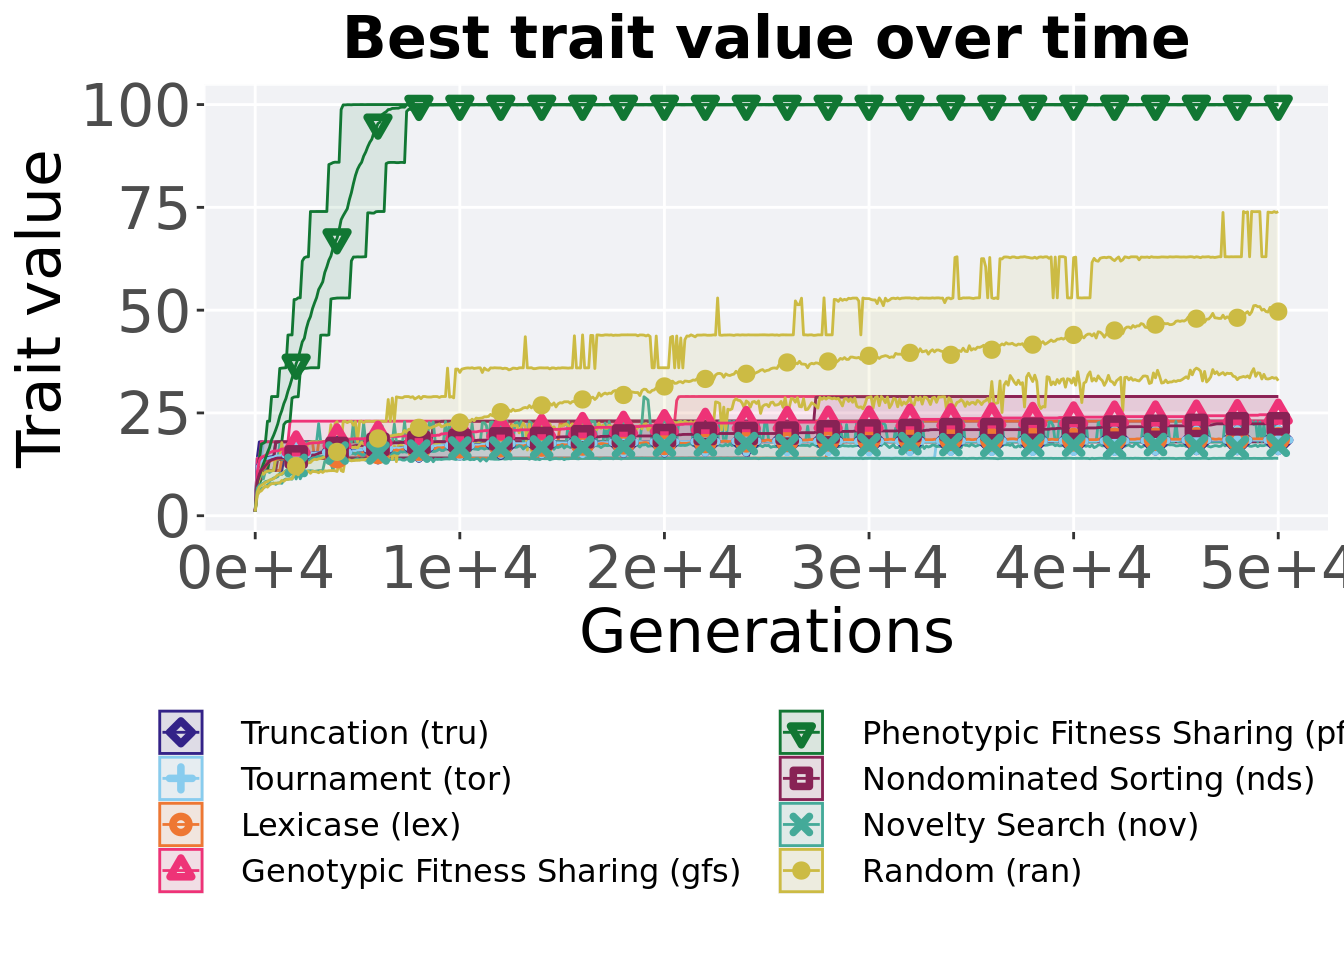
\includegraphics{mvc-diagnostics_files/figure-latex/con-per-ot-1.pdf}

\hypertarget{best-trait-value-throughout}{%
\section{Best trait value throughout}\label{best-trait-value-throughout}}

Best trait value reached throughout 50,000 generations in a population.

\begin{Shaded}
\begin{Highlighting}[]
\NormalTok{plot =}\StringTok{ }\KeywordTok{filter}\NormalTok{(best_df, var }\OperatorTok{==}\StringTok{ 'pop_fit_max'}\NormalTok{) }\OperatorTok
\StringTok{  }\KeywordTok{ggplot}\NormalTok{(., }\KeywordTok{aes}\NormalTok{(}\DataTypeTok{x =}\NormalTok{ acro, }\DataTypeTok{y =}\NormalTok{ val, }\DataTypeTok{color =}\NormalTok{ acro, }\DataTypeTok{fill =}\NormalTok{ acro, }\DataTypeTok{shape =}\NormalTok{ acro)) }\OperatorTok{+}
\StringTok{  }\KeywordTok{geom_flat_violin}\NormalTok{(}\DataTypeTok{position =} \KeywordTok{position_nudge}\NormalTok{(}\DataTypeTok{x =} \FloatTok{.09}\NormalTok{, }\DataTypeTok{y =} \DecValTok{0}\NormalTok{), }\DataTypeTok{scale =} \StringTok{'width'}\NormalTok{, }\DataTypeTok{alpha =} \FloatTok{0.2}\NormalTok{, }\DataTypeTok{width =} \FloatTok{1.5}\NormalTok{) }\OperatorTok{+}
\StringTok{  }\KeywordTok{geom_boxplot}\NormalTok{(}\DataTypeTok{color =} \StringTok{'black'}\NormalTok{, }\DataTypeTok{width =} \FloatTok{.07}\NormalTok{, }\DataTypeTok{outlier.shape =} \OtherTok{NA}\NormalTok{, }\DataTypeTok{alpha =} \FloatTok{0.0}\NormalTok{, }\DataTypeTok{size =} \FloatTok{1.0}\NormalTok{, }\DataTypeTok{position =} \KeywordTok{position_nudge}\NormalTok{(}\DataTypeTok{x =} \FloatTok{.15}\NormalTok{, }\DataTypeTok{y =} \DecValTok{0}\NormalTok{)) }\OperatorTok{+}
\StringTok{  }\KeywordTok{geom_point}\NormalTok{(}\DataTypeTok{position =} \KeywordTok{position_jitter}\NormalTok{(}\DataTypeTok{width =} \FloatTok{.02}\NormalTok{), }\DataTypeTok{size =} \FloatTok{2.0}\NormalTok{, }\DataTypeTok{alpha =} \FloatTok{1.0}\NormalTok{) }\OperatorTok{+}
\StringTok{  }\KeywordTok{scale_y_continuous}\NormalTok{(}
    \DataTypeTok{name=}\StringTok{"Average trait score"}\NormalTok{,}
    \DataTypeTok{limits=}\KeywordTok{c}\NormalTok{(}\DecValTok{0}\NormalTok{, }\DecValTok{100}\NormalTok{),}
    \DataTypeTok{breaks=}\KeywordTok{seq}\NormalTok{(}\DecValTok{0}\NormalTok{,}\DecValTok{100}\NormalTok{, }\DecValTok{20}\NormalTok{),}
    \DataTypeTok{labels=}\KeywordTok{c}\NormalTok{(}\StringTok{"0"}\NormalTok{, }\StringTok{"20"}\NormalTok{, }\StringTok{"40"}\NormalTok{, }\StringTok{"60"}\NormalTok{, }\StringTok{"80"}\NormalTok{, }\StringTok{"100"}\NormalTok{)}
\NormalTok{  ) }\OperatorTok{+}
\StringTok{  }\KeywordTok{scale_x_discrete}\NormalTok{(}
    \DataTypeTok{name=}\StringTok{"Scheme"}
\NormalTok{  )}\OperatorTok{+}
\StringTok{  }\KeywordTok{scale_shape_manual}\NormalTok{(}\DataTypeTok{values=}\NormalTok{SHAPE)}\OperatorTok{+}
\StringTok{  }\KeywordTok{scale_colour_manual}\NormalTok{(}\DataTypeTok{values =}\NormalTok{ cb_palette, ) }\OperatorTok{+}
\StringTok{  }\KeywordTok{scale_fill_manual}\NormalTok{(}\DataTypeTok{values =}\NormalTok{ cb_palette) }\OperatorTok{+}
\StringTok{  }\KeywordTok{ggtitle}\NormalTok{(}\StringTok{'Best trait value throughout'}\NormalTok{)}\OperatorTok{+}
\StringTok{  }\NormalTok{p_theme }\OperatorTok{+}\StringTok{ }\KeywordTok{theme}\NormalTok{(}\DataTypeTok{legend.title=}\KeywordTok{element_blank}\NormalTok{())}

\KeywordTok{plot_grid}\NormalTok{(}
\NormalTok{  plot }\OperatorTok{+}
\StringTok{    }\KeywordTok{theme}\NormalTok{(}\DataTypeTok{legend.position=}\StringTok{"none"}\NormalTok{),}
\NormalTok{  legend,}
  \DataTypeTok{nrow=}\DecValTok{2}\NormalTok{,}
  \DataTypeTok{rel_heights =} \KeywordTok{c}\NormalTok{(}\DecValTok{3}\NormalTok{,}\DecValTok{1}\NormalTok{)}
\NormalTok{)}
\end{Highlighting}
\end{Shaded}

\begin{verbatim}
## Warning: Removed 9 rows containing missing values (`geom_point()`).
\end{verbatim}

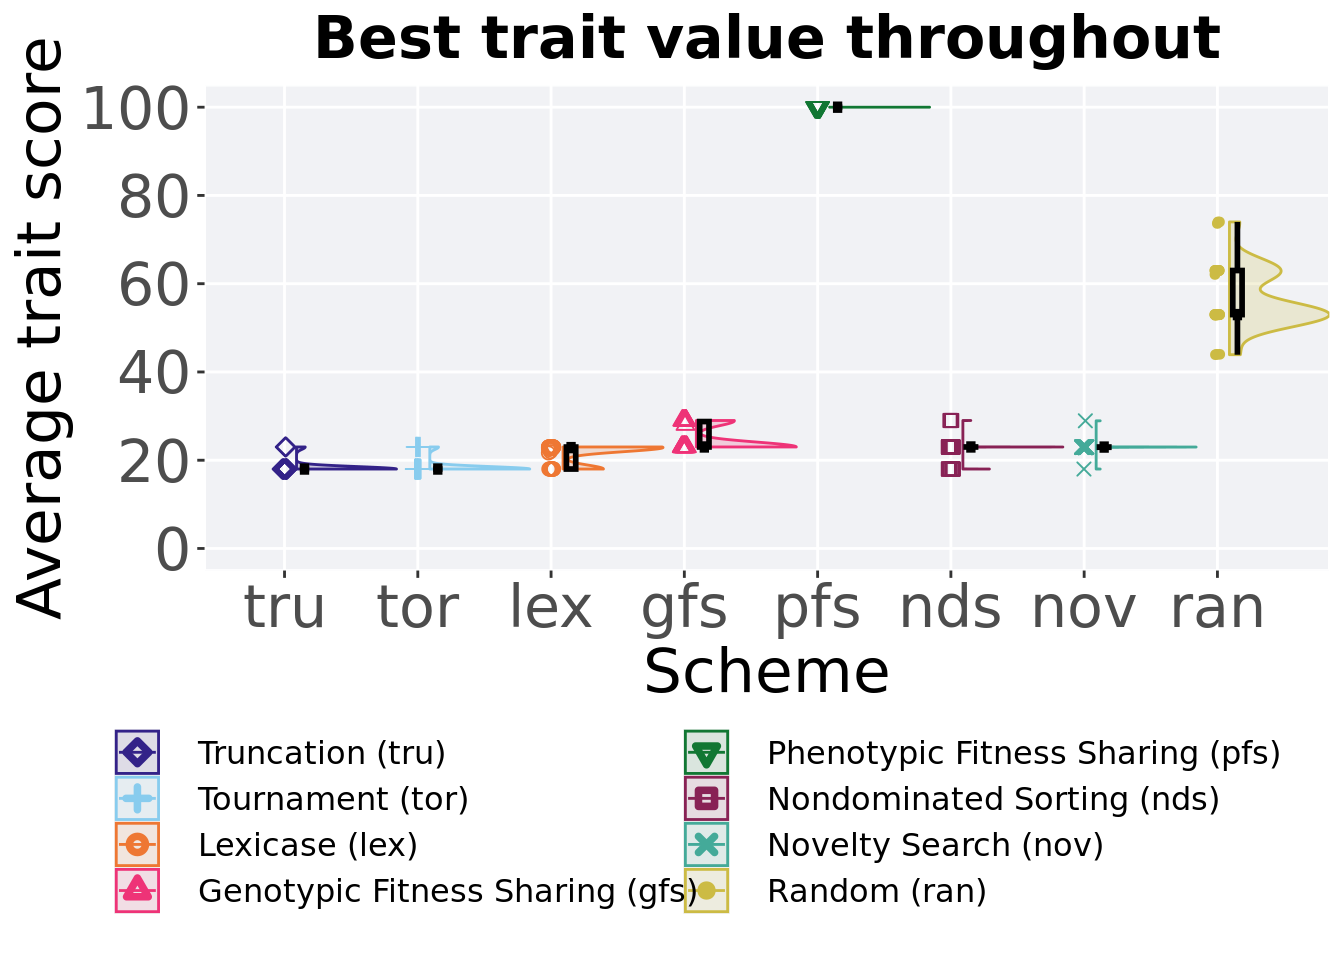
\includegraphics{mvc-diagnostics_files/figure-latex/con-per-bst-1.pdf}

\hypertarget{stats-5}{%
\subsection{Stats}\label{stats-5}}

Summary statistics for the best trait value.

\begin{Shaded}
\begin{Highlighting}[]
\NormalTok{trait_val =}\StringTok{ }\KeywordTok{filter}\NormalTok{(best_df, var }\OperatorTok{==}\StringTok{ 'pop_fit_max'}\NormalTok{)}
\NormalTok{trait_val}\OperatorTok{$}\NormalTok{acro =}\StringTok{ }\KeywordTok{factor}\NormalTok{(trait_val}\OperatorTok{$}\NormalTok{acro, }\DataTypeTok{levels =} \KeywordTok{c}\NormalTok{(}\StringTok{'pfs'}\NormalTok{,}\StringTok{'ran'}\NormalTok{,}\StringTok{'gfs'}\NormalTok{,}\StringTok{'nov'}\NormalTok{,}\StringTok{'nds'}\NormalTok{,}\StringTok{'lex'}\NormalTok{,}\StringTok{'tru'}\NormalTok{,}\StringTok{'tor'}\NormalTok{))}
\NormalTok{trait_val }\OperatorTok
\StringTok{  }\KeywordTok{group_by}\NormalTok{(acro) }\OperatorTok
\StringTok{  }\NormalTok{dplyr}\OperatorTok{::}\KeywordTok{summarise}\NormalTok{(}
    \DataTypeTok{count =} \KeywordTok{n}\NormalTok{(),}
    \DataTypeTok{na_cnt =} \KeywordTok{sum}\NormalTok{(}\KeywordTok{is.na}\NormalTok{(val)),}
    \DataTypeTok{min =} \KeywordTok{min}\NormalTok{(val, }\DataTypeTok{na.rm =} \OtherTok{TRUE}\NormalTok{),}
    \DataTypeTok{median =} \KeywordTok{median}\NormalTok{(val, }\DataTypeTok{na.rm =} \OtherTok{TRUE}\NormalTok{),}
    \DataTypeTok{mean =} \KeywordTok{mean}\NormalTok{(val, }\DataTypeTok{na.rm =} \OtherTok{TRUE}\NormalTok{),}
    \DataTypeTok{max =} \KeywordTok{max}\NormalTok{(val, }\DataTypeTok{na.rm =} \OtherTok{TRUE}\NormalTok{),}
    \DataTypeTok{IQR =} \KeywordTok{IQR}\NormalTok{(val, }\DataTypeTok{na.rm =} \OtherTok{TRUE}\NormalTok{)}
\NormalTok{  )}
\end{Highlighting}
\end{Shaded}

\begin{verbatim}
## # A tibble: 8 x 8
##   acro  count na_cnt   min median  mean   max      IQR
##   <fct> <int>  <int> <dbl>  <dbl> <dbl> <dbl>    <dbl>
## 1 pfs      50      0 100.   100   100.  100   0.000100
## 2 ran      50      0  43.9   53.0  56.7  74.0 9.99    
## 3 gfs      50      0  23.0   23    24.7  29   5.76    
## 4 nov      50      0  18.0   23.0  23.0  28.9 0.0528  
## 5 nds      50      0  18     23    22.4  29   0.00328 
## 6 lex      50      0  18     22.9  21.5  23   4.98    
## 7 tru      50      0  18.0   18    18.4  23   0       
## 8 tor      50      0  18.0   18    18.4  23   0
\end{verbatim}

Kruskal--Wallis test illustrates evidence of statistical differences.

\begin{Shaded}
\begin{Highlighting}[]
\KeywordTok{kruskal.test}\NormalTok{(val }\OperatorTok{~}\StringTok{ }\NormalTok{acro, }\DataTypeTok{data =}\NormalTok{ trait_val)}
\end{Highlighting}
\end{Shaded}

\begin{verbatim}
## 
##  Kruskal-Wallis rank sum test
## 
## data:  val by acro
## Kruskal-Wallis chi-squared = 337.68, df = 7, p-value < 2.2e-16
\end{verbatim}

Results for post-hoc Wilcoxon rank-sum test with a Bonferroni correction.

\begin{Shaded}
\begin{Highlighting}[]
\KeywordTok{pairwise.wilcox.test}\NormalTok{(}\DataTypeTok{x =}\NormalTok{ trait_val}\OperatorTok{$}\NormalTok{val, }\DataTypeTok{g =}\NormalTok{ trait_val}\OperatorTok{$}\NormalTok{acro, }\DataTypeTok{p.adjust.method =} \StringTok{"bonferroni"}\NormalTok{,}
                     \DataTypeTok{paired =} \OtherTok{FALSE}\NormalTok{, }\DataTypeTok{conf.int =} \OtherTok{FALSE}\NormalTok{, }\DataTypeTok{alternative =} \StringTok{'l'}\NormalTok{)}
\end{Highlighting}
\end{Shaded}

\begin{verbatim}
## 
##  Pairwise comparisons using Wilcoxon rank sum test with continuity correction 
## 
## data:  trait_val$val and trait_val$acro 
## 
##     pfs     ran     gfs     nov     nds     lex     tru    
## ran < 2e-16 -       -       -       -       -       -      
## gfs < 2e-16 < 2e-16 -       -       -       -       -      
## nov < 2e-16 < 2e-16 3.2e-16 -       -       -       -      
## nds < 2e-16 < 2e-16 0.00015 1.00000 -       -       -      
## lex < 2e-16 < 2e-16 3.7e-15 0.00722 1.4e-05 -       -      
## tru < 2e-16 < 2e-16 < 2e-16 4.5e-12 3.0e-11 1.0e-07 -      
## tor < 2e-16 < 2e-16 < 2e-16 6.3e-12 7.2e-11 9.4e-08 1.00000
## 
## P value adjustment method: bonferroni
\end{verbatim}

\hypertarget{multi-path-exploration-results}{%
\chapter{Multi-path exploration results}\label{multi-path-exploration-results}}

Here we present the results for \textbf{best performances} found by each selection scheme on the multi-path exploration diagnostic with valley crossing integrated.
50 replicates are conducted for each scheme explored.

\hypertarget{analysis-dependencies-3}{%
\section{Analysis dependencies}\label{analysis-dependencies-3}}

\begin{Shaded}
\begin{Highlighting}[]
\KeywordTok{library}\NormalTok{(ggplot2)}
\KeywordTok{library}\NormalTok{(cowplot)}
\KeywordTok{library}\NormalTok{(dplyr)}
\KeywordTok{library}\NormalTok{(PupillometryR)}
\end{Highlighting}
\end{Shaded}

\hypertarget{data-setup-3}{%
\section{Data setup}\label{data-setup-3}}

\begin{Shaded}
\begin{Highlighting}[]
\NormalTok{DIR =}\StringTok{ }\KeywordTok{paste}\NormalTok{(DATA_DIR,}\StringTok{'MULTIPATH_EXPLORATION/'}\NormalTok{, }\DataTypeTok{sep =} \StringTok{""}\NormalTok{, }\DataTypeTok{collapse =} \OtherTok{NULL}\NormalTok{)}
\NormalTok{over_time_df <-}\StringTok{ }\KeywordTok{read.csv}\NormalTok{(}\KeywordTok{paste}\NormalTok{(DIR,}\StringTok{'over-time.csv'}\NormalTok{, }\DataTypeTok{sep =} \StringTok{""}\NormalTok{, }\DataTypeTok{collapse =} \OtherTok{NULL}\NormalTok{), }\DataTypeTok{header =} \OtherTok{TRUE}\NormalTok{, }\DataTypeTok{stringsAsFactors =} \OtherTok{FALSE}\NormalTok{)}
\NormalTok{over_time_df}\OperatorTok{$}\NormalTok{uni_str_pos =}\StringTok{ }\NormalTok{over_time_df}\OperatorTok{$}\NormalTok{uni_str_pos }\OperatorTok{+}\StringTok{ }\NormalTok{over_time_df}\OperatorTok{$}\NormalTok{arc_acti_gene }\OperatorTok{-}\StringTok{ }\NormalTok{over_time_df}\OperatorTok{$}\NormalTok{overlap}
\NormalTok{over_time_df}\OperatorTok{$}\NormalTok{scheme <-}\StringTok{ }\KeywordTok{factor}\NormalTok{(over_time_df}\OperatorTok{$}\NormalTok{scheme, }\DataTypeTok{levels =}\NormalTok{ NAMES)}
\NormalTok{over_time_df}\OperatorTok{$}\NormalTok{acro <-}\StringTok{ }\KeywordTok{factor}\NormalTok{(over_time_df}\OperatorTok{$}\NormalTok{acro, }\DataTypeTok{levels =}\NormalTok{ ACRO)}

\NormalTok{best_df <-}\StringTok{ }\KeywordTok{read.csv}\NormalTok{(}\KeywordTok{paste}\NormalTok{(DIR,}\StringTok{'best.csv'}\NormalTok{, }\DataTypeTok{sep =} \StringTok{""}\NormalTok{, }\DataTypeTok{collapse =} \OtherTok{NULL}\NormalTok{), }\DataTypeTok{header =} \OtherTok{TRUE}\NormalTok{, }\DataTypeTok{stringsAsFactors =} \OtherTok{FALSE}\NormalTok{)}
\NormalTok{best_df}\OperatorTok{$}\NormalTok{acro <-}\StringTok{ }\KeywordTok{factor}\NormalTok{(best_df}\OperatorTok{$}\NormalTok{acro, }\DataTypeTok{levels =}\NormalTok{ ACRO)}
\end{Highlighting}
\end{Shaded}

\hypertarget{activation-gene-coverage-over-time-1}{%
\section{Activation gene coverage over time}\label{activation-gene-coverage-over-time-1}}

Activation gene coverage in a population over time.
Data points on the graph is the average activation gene coverage across 50 replicates every 2000 generations.
Shading comes from the best and worse coverage across 50 replicates.

\begin{Shaded}
\begin{Highlighting}[]
\NormalTok{lines =}\StringTok{ }\NormalTok{over_time_df }\OperatorTok
\StringTok{  }\KeywordTok{group_by}\NormalTok{(scheme, gen) }\OperatorTok
\StringTok{  }\NormalTok{dplyr}\OperatorTok{::}\KeywordTok{summarise}\NormalTok{(}
    \DataTypeTok{min =} \KeywordTok{min}\NormalTok{(uni_str_pos),}
    \DataTypeTok{mean =} \KeywordTok{mean}\NormalTok{(uni_str_pos),}
    \DataTypeTok{max =} \KeywordTok{max}\NormalTok{(uni_str_pos)}
\NormalTok{  )}
\end{Highlighting}
\end{Shaded}

\begin{verbatim}
## `summarise()` has grouped output by 'scheme'. You can override using the
## `.groups` argument.
\end{verbatim}

\begin{Shaded}
\begin{Highlighting}[]
\NormalTok{over_time_plot =}\StringTok{ }\KeywordTok{ggplot}\NormalTok{(lines, }\KeywordTok{aes}\NormalTok{(}\DataTypeTok{x=}\NormalTok{gen, }\DataTypeTok{y=}\NormalTok{mean, }\DataTypeTok{group =}\NormalTok{ scheme, }\DataTypeTok{fill =}\NormalTok{ scheme, }\DataTypeTok{color =}\NormalTok{ scheme, }\DataTypeTok{shape =}\NormalTok{ scheme)) }\OperatorTok{+}
\StringTok{  }\KeywordTok{geom_ribbon}\NormalTok{(}\KeywordTok{aes}\NormalTok{(}\DataTypeTok{ymin =}\NormalTok{ min, }\DataTypeTok{ymax =}\NormalTok{ max), }\DataTypeTok{alpha =} \FloatTok{0.1}\NormalTok{) }\OperatorTok{+}
\StringTok{  }\KeywordTok{geom_line}\NormalTok{(}\DataTypeTok{size =} \FloatTok{0.5}\NormalTok{) }\OperatorTok{+}
\StringTok{  }\KeywordTok{geom_point}\NormalTok{(}\DataTypeTok{data =} \KeywordTok{filter}\NormalTok{(lines, gen }\OperatorTok\StringTok{ }\DecValTok{2000} \OperatorTok{==}\StringTok{ }\DecValTok{0} \OperatorTok{&}\StringTok{ }\NormalTok{gen }\OperatorTok{!=}\StringTok{ }\DecValTok{0}\NormalTok{), }\DataTypeTok{size =} \FloatTok{1.5}\NormalTok{, }\DataTypeTok{stroke =} \FloatTok{2.0}\NormalTok{, }\DataTypeTok{alpha =} \FloatTok{1.0}\NormalTok{) }\OperatorTok{+}
\StringTok{  }\KeywordTok{scale_y_continuous}\NormalTok{(}
    \DataTypeTok{name=}\StringTok{"Coverage"}\NormalTok{,}
    \DataTypeTok{limits=}\KeywordTok{c}\NormalTok{(}\DecValTok{0}\NormalTok{, }\DecValTok{100}\NormalTok{),}
    \DataTypeTok{breaks=}\KeywordTok{seq}\NormalTok{(}\DecValTok{0}\NormalTok{,}\DecValTok{100}\NormalTok{, }\DecValTok{20}\NormalTok{),}
    \DataTypeTok{labels=}\KeywordTok{c}\NormalTok{(}\StringTok{"0"}\NormalTok{, }\StringTok{"20"}\NormalTok{, }\StringTok{"40"}\NormalTok{, }\StringTok{"60"}\NormalTok{, }\StringTok{"80"}\NormalTok{, }\StringTok{"100"}\NormalTok{)}
\NormalTok{  ) }\OperatorTok{+}
\StringTok{  }\KeywordTok{scale_x_continuous}\NormalTok{(}
    \DataTypeTok{name=}\StringTok{"Generations"}\NormalTok{,}
    \DataTypeTok{limits=}\KeywordTok{c}\NormalTok{(}\DecValTok{0}\NormalTok{, }\DecValTok{50000}\NormalTok{),}
    \DataTypeTok{breaks=}\KeywordTok{c}\NormalTok{(}\DecValTok{0}\NormalTok{, }\DecValTok{10000}\NormalTok{, }\DecValTok{20000}\NormalTok{, }\DecValTok{30000}\NormalTok{, }\DecValTok{40000}\NormalTok{, }\DecValTok{50000}\NormalTok{),}
    \DataTypeTok{labels=}\KeywordTok{c}\NormalTok{(}\StringTok{"0e+4"}\NormalTok{, }\StringTok{"1e+4"}\NormalTok{, }\StringTok{"2e+4"}\NormalTok{, }\StringTok{"3e+4"}\NormalTok{, }\StringTok{"4e+4"}\NormalTok{, }\StringTok{"5e+4"}\NormalTok{)}

\NormalTok{  ) }\OperatorTok{+}
\StringTok{  }\KeywordTok{scale_shape_manual}\NormalTok{(}\DataTypeTok{values=}\NormalTok{SHAPE)}\OperatorTok{+}
\StringTok{  }\KeywordTok{scale_colour_manual}\NormalTok{(}\DataTypeTok{values =}\NormalTok{ cb_palette) }\OperatorTok{+}
\StringTok{  }\KeywordTok{scale_fill_manual}\NormalTok{(}\DataTypeTok{values =}\NormalTok{ cb_palette) }\OperatorTok{+}
\StringTok{  }\KeywordTok{ggtitle}\NormalTok{(}\StringTok{'Activation gene coverage over time'}\NormalTok{)}\OperatorTok{+}
\StringTok{  }\NormalTok{p_theme }\OperatorTok{+}\StringTok{ }\KeywordTok{theme}\NormalTok{(}\DataTypeTok{legend.title=}\KeywordTok{element_blank}\NormalTok{(),}\DataTypeTok{legend.text=}\KeywordTok{element_text}\NormalTok{(}\DataTypeTok{size=}\DecValTok{12}\NormalTok{)) }\OperatorTok{+}
\StringTok{  }\KeywordTok{guides}\NormalTok{(}
    \DataTypeTok{shape=}\KeywordTok{guide_legend}\NormalTok{(}\DataTypeTok{ncol=}\DecValTok{2}\NormalTok{, }\DataTypeTok{title.position =} \StringTok{"bottom"}\NormalTok{),}
    \DataTypeTok{color=}\KeywordTok{guide_legend}\NormalTok{(}\DataTypeTok{ncol=}\DecValTok{2}\NormalTok{, }\DataTypeTok{title.position =} \StringTok{"bottom"}\NormalTok{),}
    \DataTypeTok{fill=}\KeywordTok{guide_legend}\NormalTok{(}\DataTypeTok{ncol=}\DecValTok{2}\NormalTok{, }\DataTypeTok{title.position =} \StringTok{"bottom"}\NormalTok{)}
\NormalTok{  )}

\NormalTok{over_time_plot}
\end{Highlighting}
\end{Shaded}

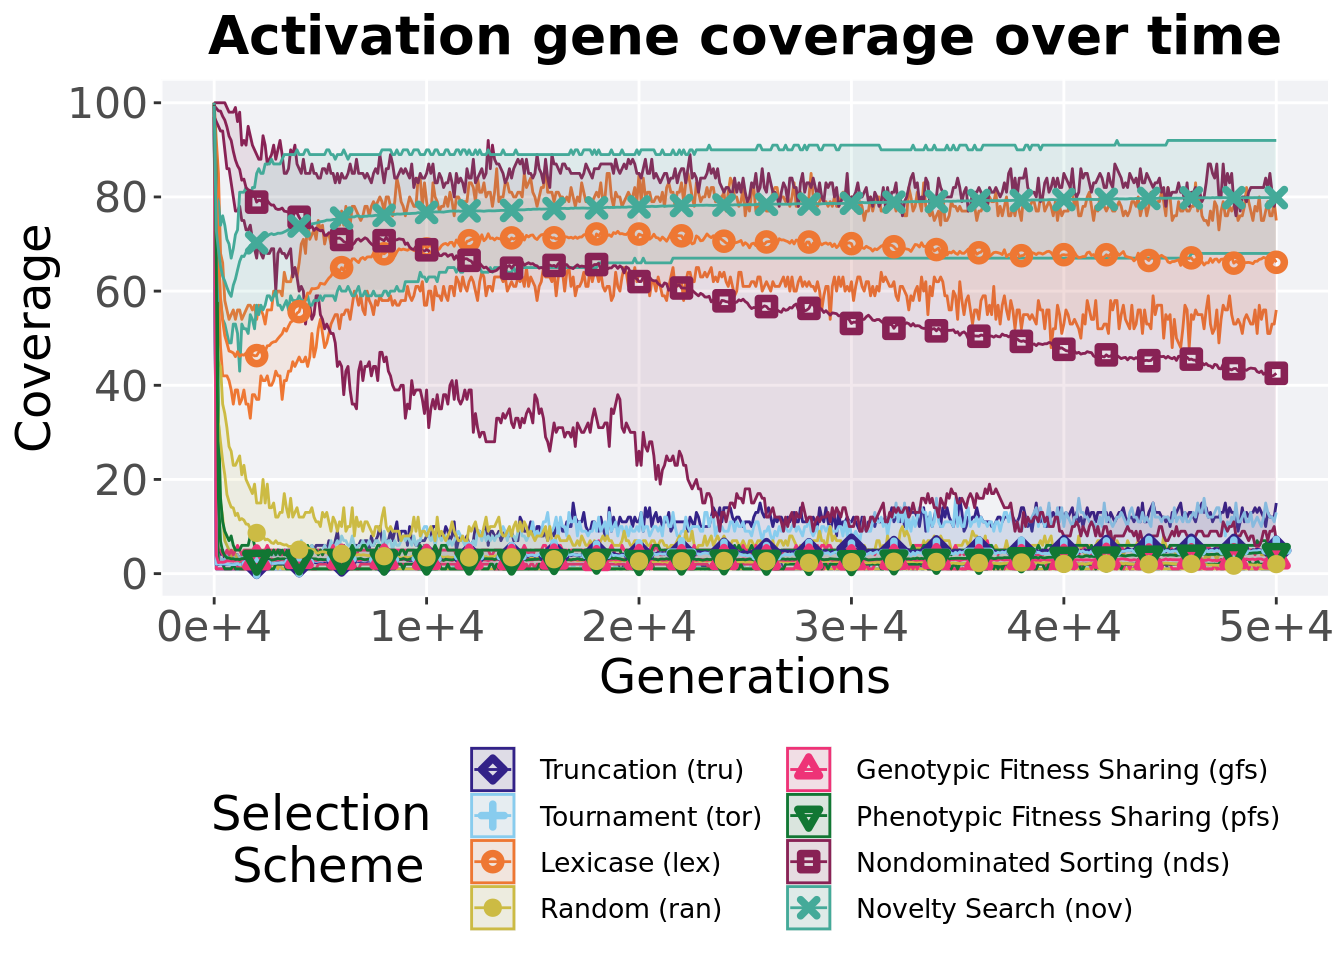
\includegraphics{mvc-diagnostics_files/figure-latex/mul-act-ot-1.pdf}

\hypertarget{final-activation-gene-coverage-1}{%
\section{Final activation gene coverage}\label{final-activation-gene-coverage-1}}

Activation gene coverage found in the final population at 50,000 generations.

\begin{Shaded}
\begin{Highlighting}[]
\NormalTok{plot =}\StringTok{ }\KeywordTok{filter}\NormalTok{(over_time_df, gen }\OperatorTok{==}\StringTok{ }\DecValTok{50000}\NormalTok{) }\OperatorTok
\StringTok{  }\KeywordTok{ggplot}\NormalTok{(., }\KeywordTok{aes}\NormalTok{(}\DataTypeTok{x =}\NormalTok{ acro, }\DataTypeTok{y =}\NormalTok{ uni_str_pos, }\DataTypeTok{color =}\NormalTok{ acro, }\DataTypeTok{fill =}\NormalTok{ acro, }\DataTypeTok{shape =}\NormalTok{ acro)) }\OperatorTok{+}
\StringTok{  }\KeywordTok{geom_flat_violin}\NormalTok{(}\DataTypeTok{position =} \KeywordTok{position_nudge}\NormalTok{(}\DataTypeTok{x =} \FloatTok{.09}\NormalTok{, }\DataTypeTok{y =} \DecValTok{0}\NormalTok{), }\DataTypeTok{scale =} \StringTok{'width'}\NormalTok{, }\DataTypeTok{alpha =} \FloatTok{0.2}\NormalTok{, }\DataTypeTok{width =} \FloatTok{1.5}\NormalTok{) }\OperatorTok{+}
\StringTok{  }\KeywordTok{geom_boxplot}\NormalTok{(}\DataTypeTok{color =} \StringTok{'black'}\NormalTok{, }\DataTypeTok{width =} \FloatTok{.07}\NormalTok{, }\DataTypeTok{outlier.shape =} \OtherTok{NA}\NormalTok{, }\DataTypeTok{alpha =} \FloatTok{0.0}\NormalTok{, }\DataTypeTok{size =} \FloatTok{1.0}\NormalTok{, }\DataTypeTok{position =} \KeywordTok{position_nudge}\NormalTok{(}\DataTypeTok{x =} \FloatTok{.15}\NormalTok{, }\DataTypeTok{y =} \DecValTok{0}\NormalTok{)) }\OperatorTok{+}
\StringTok{  }\KeywordTok{geom_point}\NormalTok{(}\DataTypeTok{position =} \KeywordTok{position_jitter}\NormalTok{(}\DataTypeTok{width =} \FloatTok{0.01}\NormalTok{, }\DataTypeTok{height =} \FloatTok{0.1}\NormalTok{), }\DataTypeTok{size =} \FloatTok{2.0}\NormalTok{, }\DataTypeTok{alpha =} \FloatTok{1.0}\NormalTok{) }\OperatorTok{+}
\StringTok{  }\KeywordTok{scale_y_continuous}\NormalTok{(}
    \DataTypeTok{name=}\StringTok{"Coverage"}\NormalTok{,}
    \DataTypeTok{limits=}\KeywordTok{c}\NormalTok{(}\DecValTok{0}\NormalTok{, }\DecValTok{100}\NormalTok{),}
    \DataTypeTok{breaks=}\KeywordTok{seq}\NormalTok{(}\DecValTok{0}\NormalTok{,}\DecValTok{100}\NormalTok{, }\DecValTok{20}\NormalTok{),}
    \DataTypeTok{labels=}\KeywordTok{c}\NormalTok{(}\StringTok{"0"}\NormalTok{, }\StringTok{"20"}\NormalTok{, }\StringTok{"40"}\NormalTok{, }\StringTok{"60"}\NormalTok{, }\StringTok{"80"}\NormalTok{, }\StringTok{"100"}\NormalTok{)}
\NormalTok{  ) }\OperatorTok{+}
\StringTok{  }\KeywordTok{scale_x_discrete}\NormalTok{(}
    \DataTypeTok{name=}\StringTok{"Scheme"}
\NormalTok{  )}\OperatorTok{+}
\StringTok{  }\KeywordTok{scale_shape_manual}\NormalTok{(}\DataTypeTok{values=}\NormalTok{SHAPE)}\OperatorTok{+}
\StringTok{  }\KeywordTok{scale_colour_manual}\NormalTok{(}\DataTypeTok{values =}\NormalTok{ cb_palette, ) }\OperatorTok{+}
\StringTok{  }\KeywordTok{scale_fill_manual}\NormalTok{(}\DataTypeTok{values =}\NormalTok{ cb_palette) }\OperatorTok{+}
\StringTok{  }\KeywordTok{ggtitle}\NormalTok{(}\StringTok{'Final activation gene coverage'}\NormalTok{)}\OperatorTok{+}
\StringTok{  }\NormalTok{p_theme }\OperatorTok{+}\StringTok{ }\KeywordTok{theme}\NormalTok{(}\DataTypeTok{legend.title=}\KeywordTok{element_blank}\NormalTok{())}

\KeywordTok{plot_grid}\NormalTok{(}
\NormalTok{  plot }\OperatorTok{+}
\StringTok{    }\KeywordTok{theme}\NormalTok{(}\DataTypeTok{legend.position=}\StringTok{"none"}\NormalTok{),}
\NormalTok{  legend,}
  \DataTypeTok{nrow=}\DecValTok{2}\NormalTok{,}
  \DataTypeTok{rel_heights =} \KeywordTok{c}\NormalTok{(}\DecValTok{3}\NormalTok{,}\DecValTok{1}\NormalTok{)}
\NormalTok{)}
\end{Highlighting}
\end{Shaded}

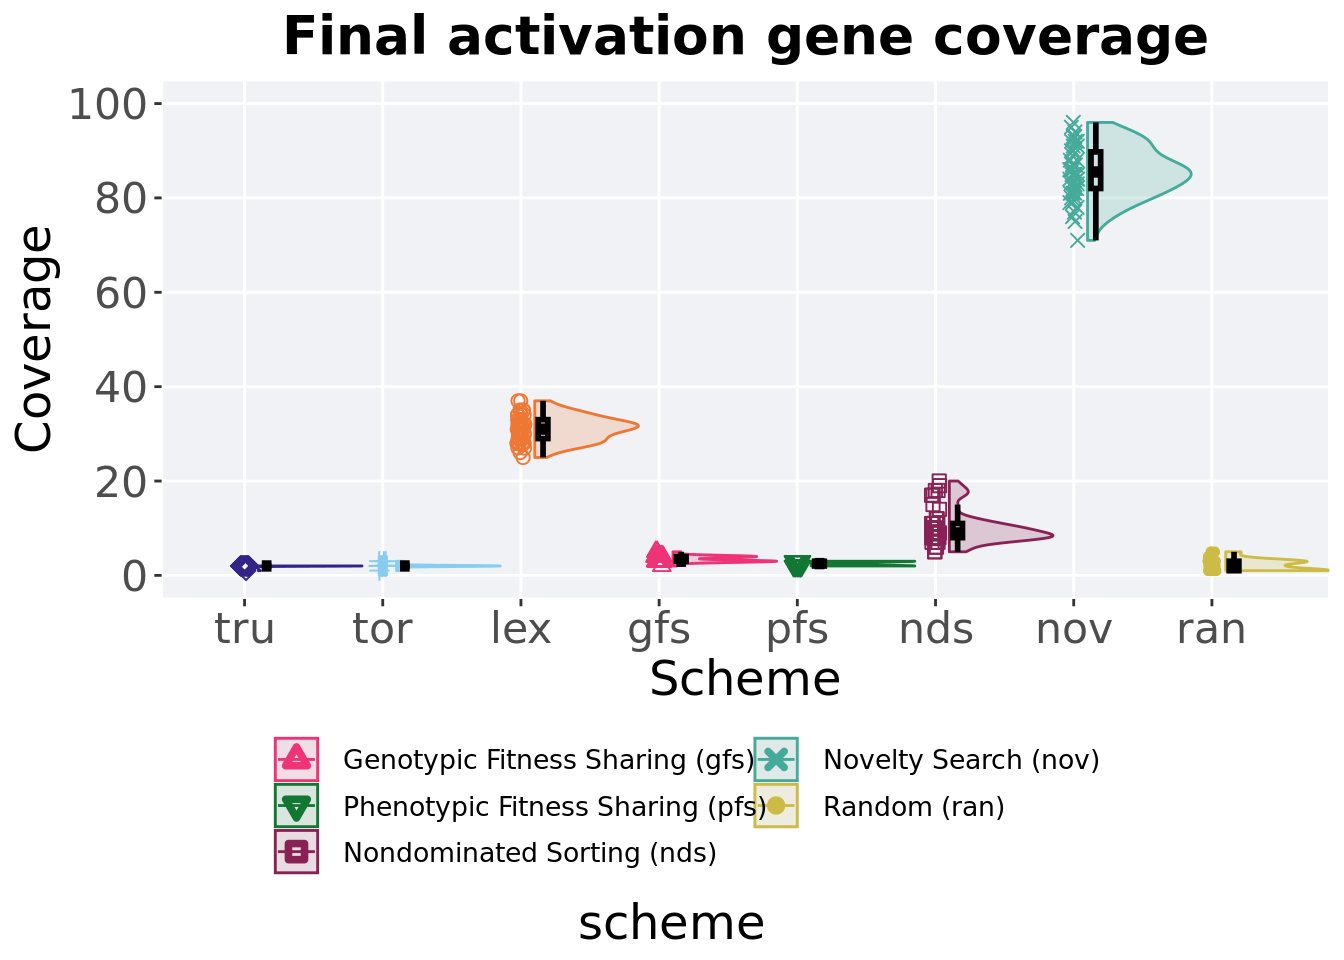
\includegraphics{mvc-diagnostics_files/figure-latex/mul-act-end-1.pdf}

\hypertarget{stats-6}{%
\subsection{Stats}\label{stats-6}}

Summary statistics for the coverage found in the final population.

\begin{Shaded}
\begin{Highlighting}[]
\NormalTok{act_coverage =}\StringTok{ }\KeywordTok{filter}\NormalTok{(over_time_df, gen }\OperatorTok{==}\StringTok{ }\DecValTok{50000}\NormalTok{)}
\NormalTok{act_coverage}\OperatorTok{$}\NormalTok{acro =}\StringTok{ }\KeywordTok{factor}\NormalTok{(act_coverage}\OperatorTok{$}\NormalTok{acro, }\DataTypeTok{levels =} \KeywordTok{c}\NormalTok{(}\StringTok{'nov'}\NormalTok{,}\StringTok{'lex'}\NormalTok{,}\StringTok{'nds'}\NormalTok{,}\StringTok{'tor'}\NormalTok{,}\StringTok{'tru'}\NormalTok{,}\StringTok{'gfs'}\NormalTok{,}\StringTok{'pfs'}\NormalTok{,}\StringTok{'ran'}\NormalTok{))}
\NormalTok{act_coverage }\OperatorTok
\StringTok{  }\KeywordTok{group_by}\NormalTok{(acro) }\OperatorTok
\StringTok{  }\NormalTok{dplyr}\OperatorTok{::}\KeywordTok{summarise}\NormalTok{(}
    \DataTypeTok{count =} \KeywordTok{n}\NormalTok{(),}
    \DataTypeTok{na_cnt =} \KeywordTok{sum}\NormalTok{(}\KeywordTok{is.na}\NormalTok{(uni_str_pos)),}
    \DataTypeTok{min =} \KeywordTok{min}\NormalTok{(uni_str_pos, }\DataTypeTok{na.rm =} \OtherTok{TRUE}\NormalTok{),}
    \DataTypeTok{median =} \KeywordTok{median}\NormalTok{(uni_str_pos, }\DataTypeTok{na.rm =} \OtherTok{TRUE}\NormalTok{),}
    \DataTypeTok{mean =} \KeywordTok{mean}\NormalTok{(uni_str_pos, }\DataTypeTok{na.rm =} \OtherTok{TRUE}\NormalTok{),}
    \DataTypeTok{max =} \KeywordTok{max}\NormalTok{(uni_str_pos, }\DataTypeTok{na.rm =} \OtherTok{TRUE}\NormalTok{),}
    \DataTypeTok{IQR =} \KeywordTok{IQR}\NormalTok{(uni_str_pos, }\DataTypeTok{na.rm =} \OtherTok{TRUE}\NormalTok{)}
\NormalTok{  )}
\end{Highlighting}
\end{Shaded}

\begin{verbatim}
## # A tibble: 8 x 8
##   acro  count na_cnt   min median  mean   max   IQR
##   <fct> <int>  <int> <int>  <dbl> <dbl> <int> <dbl>
## 1 nov      50      0    65   79   78.4     89  6.75
## 2 lex      50      0    56   67   66.5     77  6   
## 3 nds      50      0    12   43.5 41.0     82 35.8 
## 4 tor      50      0     1    4    4.4     10  3   
## 5 tru      50      0     1    4    4.28    10  2   
## 6 gfs      50      0     1    3    2.88     5  1   
## 7 pfs      50      0     2    5    4.64     7  1   
## 8 ran      50      0     1    2    1.98     5  2
\end{verbatim}

Kruskal--Wallis test illustrates evidence of statistical differences.

\begin{Shaded}
\begin{Highlighting}[]
\KeywordTok{kruskal.test}\NormalTok{(uni_str_pos }\OperatorTok{~}\StringTok{ }\NormalTok{acro, }\DataTypeTok{data =}\NormalTok{ act_coverage)}
\end{Highlighting}
\end{Shaded}

\begin{verbatim}
## 
##  Kruskal-Wallis rank sum test
## 
## data:  uni_str_pos by acro
## Kruskal-Wallis chi-squared = 333.43, df = 7, p-value < 2.2e-16
\end{verbatim}

Results for post-hoc Wilcoxon rank-sum test with a Bonferroni correction.

\begin{Shaded}
\begin{Highlighting}[]
\KeywordTok{pairwise.wilcox.test}\NormalTok{(}\DataTypeTok{x =}\NormalTok{ act_coverage}\OperatorTok{$}\NormalTok{uni_str_pos, }\DataTypeTok{g =}\NormalTok{ act_coverage}\OperatorTok{$}\NormalTok{acro, }\DataTypeTok{p.adjust.method =} \StringTok{"bonferroni"}\NormalTok{,}
                     \DataTypeTok{paired =} \OtherTok{FALSE}\NormalTok{, }\DataTypeTok{conf.int =} \OtherTok{FALSE}\NormalTok{, }\DataTypeTok{alternative =} \StringTok{'l'}\NormalTok{)}
\end{Highlighting}
\end{Shaded}

\begin{verbatim}
## 
##  Pairwise comparisons using Wilcoxon rank sum test with continuity correction 
## 
## data:  act_coverage$uni_str_pos and act_coverage$acro 
## 
##     nov     lex     nds     tor     tru     gfs     pfs    
## lex 3.0e-14 -       -       -       -       -       -      
## nds 1.5e-14 2.0e-09 -       -       -       -       -      
## tor < 2e-16 < 2e-16 < 2e-16 -       -       -       -      
## tru < 2e-16 < 2e-16 < 2e-16 1.0000  -       -       -      
## gfs < 2e-16 < 2e-16 < 2e-16 0.0032  0.0012  -       -      
## pfs < 2e-16 < 2e-16 < 2e-16 1.0000  1.0000  1.0000  -      
## ran < 2e-16 < 2e-16 < 2e-16 1.6e-08 1.1e-08 5.8e-05 2.2e-14
## 
## P value adjustment method: bonferroni
\end{verbatim}

\hypertarget{performance-over-time-2}{%
\section{Performance over time}\label{performance-over-time-2}}

Best performance in a population over time.
Data points on the graph is the average performance across 50 replicates every 2000 generations.
Shading comes from the best and worse performance across 50 replicates.

\begin{Shaded}
\begin{Highlighting}[]
\NormalTok{lines =}\StringTok{ }\NormalTok{over_time_df }\OperatorTok
\StringTok{  }\KeywordTok{group_by}\NormalTok{(scheme, gen) }\OperatorTok
\StringTok{  }\NormalTok{dplyr}\OperatorTok{::}\KeywordTok{summarise}\NormalTok{(}
    \DataTypeTok{min =} \KeywordTok{min}\NormalTok{(pop_fit_max) }\OperatorTok{/}\StringTok{ }\NormalTok{DIMENSIONALITY,}
    \DataTypeTok{mean =} \KeywordTok{mean}\NormalTok{(pop_fit_max) }\OperatorTok{/}\StringTok{ }\NormalTok{DIMENSIONALITY,}
    \DataTypeTok{max =} \KeywordTok{max}\NormalTok{(pop_fit_max) }\OperatorTok{/}\StringTok{ }\NormalTok{DIMENSIONALITY}
\NormalTok{  )}
\end{Highlighting}
\end{Shaded}

\begin{verbatim}
## `summarise()` has grouped output by 'scheme'. You can override using the
## `.groups` argument.
\end{verbatim}

\begin{Shaded}
\begin{Highlighting}[]
\NormalTok{over_time_plot =}\StringTok{ }\KeywordTok{ggplot}\NormalTok{(lines, }\KeywordTok{aes}\NormalTok{(}\DataTypeTok{x=}\NormalTok{gen, }\DataTypeTok{y=}\NormalTok{mean, }\DataTypeTok{group =}\NormalTok{ scheme, }\DataTypeTok{fill =}\NormalTok{ scheme, }\DataTypeTok{color =}\NormalTok{ scheme, }\DataTypeTok{shape =}\NormalTok{ scheme)) }\OperatorTok{+}
\StringTok{  }\KeywordTok{geom_ribbon}\NormalTok{(}\KeywordTok{aes}\NormalTok{(}\DataTypeTok{ymin =}\NormalTok{ min, }\DataTypeTok{ymax =}\NormalTok{ max), }\DataTypeTok{alpha =} \FloatTok{0.1}\NormalTok{) }\OperatorTok{+}
\StringTok{  }\KeywordTok{geom_line}\NormalTok{(}\DataTypeTok{size =} \FloatTok{0.5}\NormalTok{) }\OperatorTok{+}
\StringTok{  }\KeywordTok{geom_point}\NormalTok{(}\DataTypeTok{data =} \KeywordTok{filter}\NormalTok{(lines, gen }\OperatorTok\StringTok{ }\DecValTok{2000} \OperatorTok{==}\StringTok{ }\DecValTok{0} \OperatorTok{&}\StringTok{ }\NormalTok{gen }\OperatorTok{!=}\StringTok{ }\DecValTok{0}\NormalTok{), }\DataTypeTok{size =} \FloatTok{1.5}\NormalTok{, }\DataTypeTok{stroke =} \FloatTok{2.0}\NormalTok{, }\DataTypeTok{alpha =} \FloatTok{1.0}\NormalTok{) }\OperatorTok{+}
\StringTok{  }\KeywordTok{scale_y_continuous}\NormalTok{(}
    \DataTypeTok{name=}\StringTok{"Average trait score"}\NormalTok{,}
    \DataTypeTok{limits=}\KeywordTok{c}\NormalTok{(}\DecValTok{0}\NormalTok{, }\DecValTok{15}\NormalTok{),}
\NormalTok{  ) }\OperatorTok{+}
\StringTok{  }\KeywordTok{scale_x_continuous}\NormalTok{(}
    \DataTypeTok{name=}\StringTok{"Generations"}\NormalTok{,}
    \DataTypeTok{limits=}\KeywordTok{c}\NormalTok{(}\DecValTok{0}\NormalTok{, }\DecValTok{50000}\NormalTok{),}
    \DataTypeTok{breaks=}\KeywordTok{c}\NormalTok{(}\DecValTok{0}\NormalTok{, }\DecValTok{10000}\NormalTok{, }\DecValTok{20000}\NormalTok{, }\DecValTok{30000}\NormalTok{, }\DecValTok{40000}\NormalTok{, }\DecValTok{50000}\NormalTok{),}
    \DataTypeTok{labels=}\KeywordTok{c}\NormalTok{(}\StringTok{"0e+4"}\NormalTok{, }\StringTok{"1e+4"}\NormalTok{, }\StringTok{"2e+4"}\NormalTok{, }\StringTok{"3e+4"}\NormalTok{, }\StringTok{"4e+4"}\NormalTok{, }\StringTok{"5e+4"}\NormalTok{)}

\NormalTok{  ) }\OperatorTok{+}
\StringTok{  }\KeywordTok{scale_shape_manual}\NormalTok{(}\DataTypeTok{values=}\NormalTok{SHAPE)}\OperatorTok{+}
\StringTok{  }\KeywordTok{scale_colour_manual}\NormalTok{(}\DataTypeTok{values =}\NormalTok{ cb_palette) }\OperatorTok{+}
\StringTok{  }\KeywordTok{scale_fill_manual}\NormalTok{(}\DataTypeTok{values =}\NormalTok{ cb_palette) }\OperatorTok{+}
\StringTok{  }\KeywordTok{ggtitle}\NormalTok{(}\StringTok{'Performance over time'}\NormalTok{)}\OperatorTok{+}
\StringTok{  }\NormalTok{p_theme }\OperatorTok{+}\StringTok{ }\KeywordTok{theme}\NormalTok{(}\DataTypeTok{legend.title=}\KeywordTok{element_blank}\NormalTok{(),}\DataTypeTok{legend.text=}\KeywordTok{element_text}\NormalTok{(}\DataTypeTok{size=}\DecValTok{12}\NormalTok{)) }\OperatorTok{+}
\StringTok{  }\KeywordTok{guides}\NormalTok{(}
    \DataTypeTok{shape=}\KeywordTok{guide_legend}\NormalTok{(}\DataTypeTok{ncol=}\DecValTok{2}\NormalTok{, }\DataTypeTok{title.position =} \StringTok{"bottom"}\NormalTok{),}
    \DataTypeTok{color=}\KeywordTok{guide_legend}\NormalTok{(}\DataTypeTok{ncol=}\DecValTok{2}\NormalTok{, }\DataTypeTok{title.position =} \StringTok{"bottom"}\NormalTok{),}
    \DataTypeTok{fill=}\KeywordTok{guide_legend}\NormalTok{(}\DataTypeTok{ncol=}\DecValTok{2}\NormalTok{, }\DataTypeTok{title.position =} \StringTok{"bottom"}\NormalTok{)}
\NormalTok{  )}

\NormalTok{over_time_plot}
\end{Highlighting}
\end{Shaded}

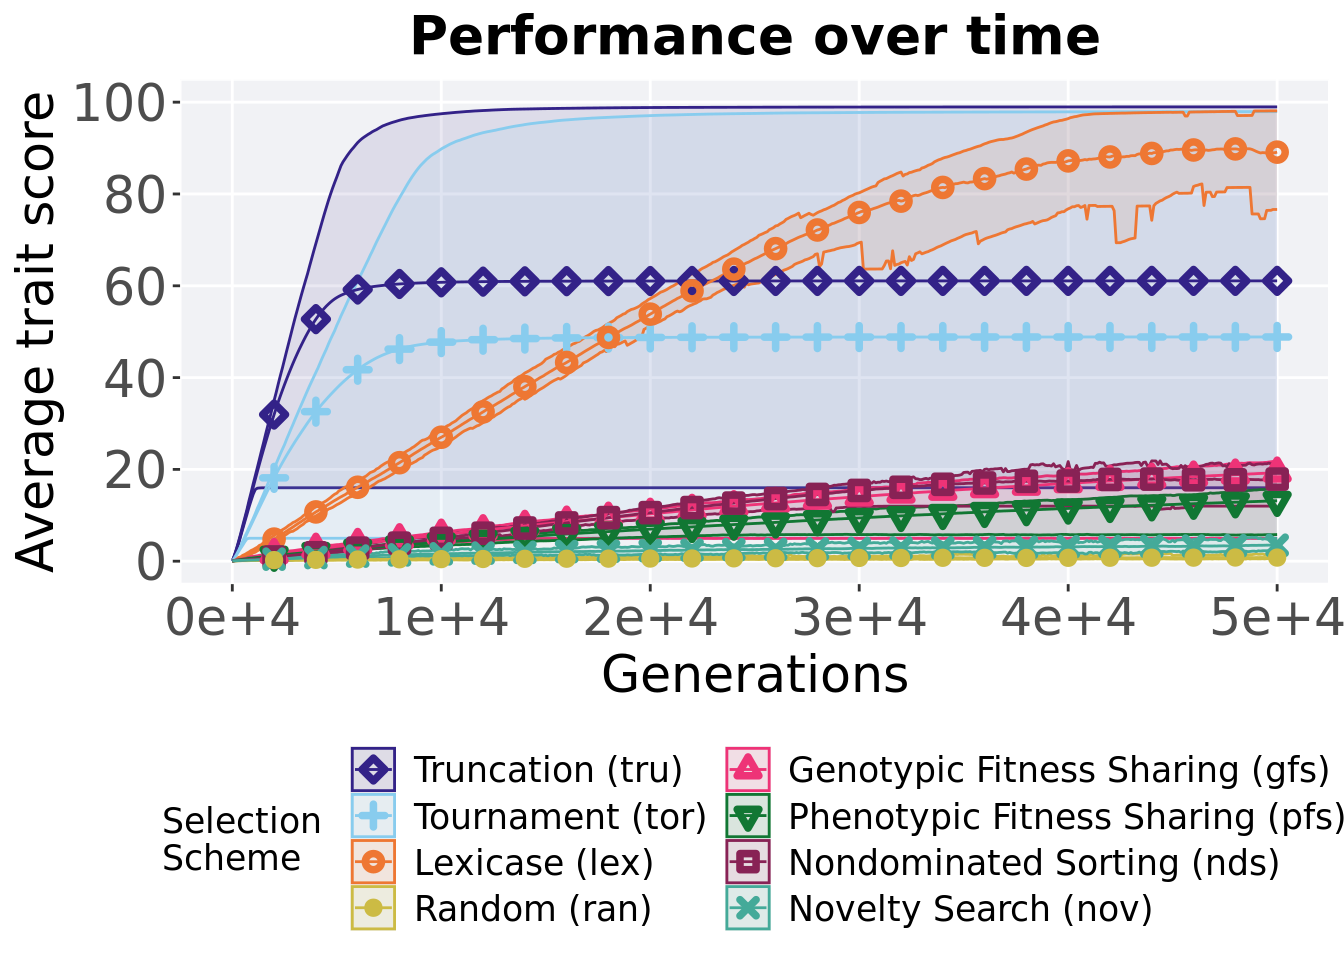
\includegraphics{mvc-diagnostics_files/figure-latex/mul-per-ot-1.pdf}

\hypertarget{best-performance-throughout-2}{%
\section{Best performance throughout}\label{best-performance-throughout-2}}

Best performance reached throughout 50,000 generations in a population.

\begin{Shaded}
\begin{Highlighting}[]
\NormalTok{plot =}\StringTok{ }\KeywordTok{filter}\NormalTok{(best_df, var }\OperatorTok{==}\StringTok{ 'pop_fit_max'}\NormalTok{) }\OperatorTok
\StringTok{  }\KeywordTok{ggplot}\NormalTok{(., }\KeywordTok{aes}\NormalTok{(}\DataTypeTok{x =}\NormalTok{ acro, }\DataTypeTok{y =}\NormalTok{ val }\OperatorTok{/}\StringTok{ }\NormalTok{DIMENSIONALITY, }\DataTypeTok{color =}\NormalTok{ acro, }\DataTypeTok{fill =}\NormalTok{ acro, }\DataTypeTok{shape =}\NormalTok{ acro)) }\OperatorTok{+}
\StringTok{  }\KeywordTok{geom_flat_violin}\NormalTok{(}\DataTypeTok{position =} \KeywordTok{position_nudge}\NormalTok{(}\DataTypeTok{x =} \FloatTok{.09}\NormalTok{, }\DataTypeTok{y =} \DecValTok{0}\NormalTok{), }\DataTypeTok{scale =} \StringTok{'width'}\NormalTok{, }\DataTypeTok{alpha =} \FloatTok{0.2}\NormalTok{, }\DataTypeTok{width =} \FloatTok{1.5}\NormalTok{) }\OperatorTok{+}
\StringTok{  }\KeywordTok{geom_boxplot}\NormalTok{(}\DataTypeTok{color =} \StringTok{'black'}\NormalTok{, }\DataTypeTok{width =} \FloatTok{.07}\NormalTok{, }\DataTypeTok{outlier.shape =} \OtherTok{NA}\NormalTok{, }\DataTypeTok{alpha =} \FloatTok{0.0}\NormalTok{, }\DataTypeTok{size =} \FloatTok{1.0}\NormalTok{, }\DataTypeTok{position =} \KeywordTok{position_nudge}\NormalTok{(}\DataTypeTok{x =} \FloatTok{.15}\NormalTok{, }\DataTypeTok{y =} \DecValTok{0}\NormalTok{)) }\OperatorTok{+}
\StringTok{  }\KeywordTok{geom_point}\NormalTok{(}\DataTypeTok{position =} \KeywordTok{position_jitter}\NormalTok{(}\DataTypeTok{width =} \FloatTok{.02}\NormalTok{), }\DataTypeTok{size =} \FloatTok{2.0}\NormalTok{, }\DataTypeTok{alpha =} \FloatTok{1.0}\NormalTok{) }\OperatorTok{+}
\StringTok{  }\KeywordTok{scale_y_continuous}\NormalTok{(}
    \DataTypeTok{name=}\StringTok{"Average trait score"}\NormalTok{,}
    \DataTypeTok{limits=}\KeywordTok{c}\NormalTok{(}\DecValTok{0}\NormalTok{, }\DecValTok{15}\NormalTok{),}
\NormalTok{  ) }\OperatorTok{+}
\StringTok{  }\KeywordTok{scale_x_discrete}\NormalTok{(}
    \DataTypeTok{name=}\StringTok{"Scheme"}
\NormalTok{  )}\OperatorTok{+}
\StringTok{  }\KeywordTok{scale_shape_manual}\NormalTok{(}\DataTypeTok{values=}\NormalTok{SHAPE)}\OperatorTok{+}
\StringTok{  }\KeywordTok{scale_colour_manual}\NormalTok{(}\DataTypeTok{values =}\NormalTok{ cb_palette, ) }\OperatorTok{+}
\StringTok{  }\KeywordTok{scale_fill_manual}\NormalTok{(}\DataTypeTok{values =}\NormalTok{ cb_palette) }\OperatorTok{+}
\StringTok{  }\KeywordTok{ggtitle}\NormalTok{(}\StringTok{'Best performance throughout'}\NormalTok{)}\OperatorTok{+}
\StringTok{  }\NormalTok{p_theme }\OperatorTok{+}\StringTok{ }\KeywordTok{theme}\NormalTok{(}\DataTypeTok{legend.title=}\KeywordTok{element_blank}\NormalTok{())}

\KeywordTok{plot_grid}\NormalTok{(}
\NormalTok{  plot }\OperatorTok{+}
\StringTok{    }\KeywordTok{theme}\NormalTok{(}\DataTypeTok{legend.position=}\StringTok{"none"}\NormalTok{),}
\NormalTok{  legend,}
  \DataTypeTok{nrow=}\DecValTok{2}\NormalTok{,}
  \DataTypeTok{rel_heights =} \KeywordTok{c}\NormalTok{(}\DecValTok{3}\NormalTok{,}\DecValTok{1}\NormalTok{)}
\NormalTok{)}
\end{Highlighting}
\end{Shaded}

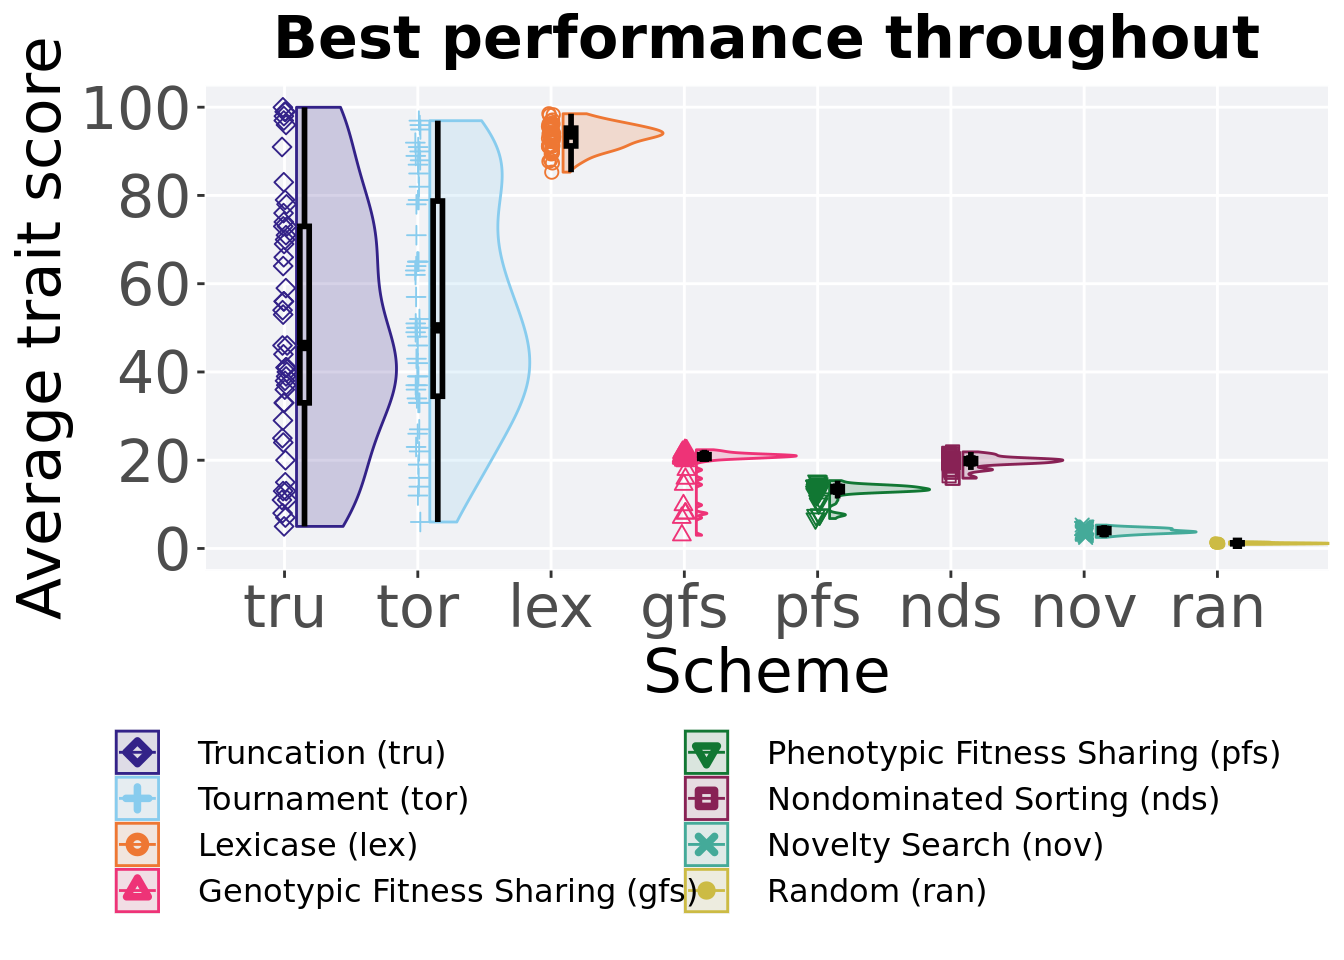
\includegraphics{mvc-diagnostics_files/figure-latex/mul-per-bst-1.pdf}

\hypertarget{stats-7}{%
\subsection{Stats}\label{stats-7}}

Summary statistics for the best performance.

\begin{Shaded}
\begin{Highlighting}[]
\NormalTok{performance =}\StringTok{ }\KeywordTok{filter}\NormalTok{(best_df, var }\OperatorTok{==}\StringTok{ 'pop_fit_max'}\NormalTok{)}
\NormalTok{performance}\OperatorTok{$}\NormalTok{acro =}\StringTok{ }\KeywordTok{factor}\NormalTok{(performance}\OperatorTok{$}\NormalTok{acro, }\DataTypeTok{levels =} \KeywordTok{c}\NormalTok{(}\StringTok{'gfs'}\NormalTok{,}\StringTok{'pfs'}\NormalTok{,}\StringTok{'tru'}\NormalTok{,}\StringTok{'tor'}\NormalTok{,}\StringTok{'nov'}\NormalTok{,}\StringTok{'lex'}\NormalTok{,}\StringTok{'nds'}\NormalTok{,}\StringTok{'ran'}\NormalTok{))}
\NormalTok{performance }\OperatorTok
\StringTok{  }\KeywordTok{group_by}\NormalTok{(acro) }\OperatorTok
\StringTok{  }\NormalTok{dplyr}\OperatorTok{::}\KeywordTok{summarise}\NormalTok{(}
    \DataTypeTok{count =} \KeywordTok{n}\NormalTok{(),}
    \DataTypeTok{na_cnt =} \KeywordTok{sum}\NormalTok{(}\KeywordTok{is.na}\NormalTok{(val)),}
    \DataTypeTok{min =} \KeywordTok{min}\NormalTok{(val }\OperatorTok{/}\StringTok{ }\NormalTok{DIMENSIONALITY, }\DataTypeTok{na.rm =} \OtherTok{TRUE}\NormalTok{),}
    \DataTypeTok{median =} \KeywordTok{median}\NormalTok{(val }\OperatorTok{/}\StringTok{ }\NormalTok{DIMENSIONALITY, }\DataTypeTok{na.rm =} \OtherTok{TRUE}\NormalTok{),}
    \DataTypeTok{mean =} \KeywordTok{mean}\NormalTok{(val }\OperatorTok{/}\StringTok{ }\NormalTok{DIMENSIONALITY, }\DataTypeTok{na.rm =} \OtherTok{TRUE}\NormalTok{),}
    \DataTypeTok{max =} \KeywordTok{max}\NormalTok{(val }\OperatorTok{/}\StringTok{ }\NormalTok{DIMENSIONALITY, }\DataTypeTok{na.rm =} \OtherTok{TRUE}\NormalTok{),}
    \DataTypeTok{IQR =} \KeywordTok{IQR}\NormalTok{(val }\OperatorTok{/}\StringTok{ }\NormalTok{DIMENSIONALITY, }\DataTypeTok{na.rm =} \OtherTok{TRUE}\NormalTok{)}
\NormalTok{  )}
\end{Highlighting}
\end{Shaded}

\begin{verbatim}
## # A tibble: 8 x 8
##   acro  count na_cnt   min median  mean   max   IQR
##   <fct> <int>  <int> <dbl>  <dbl> <dbl> <dbl> <dbl>
## 1 gfs      50      0 3.07   11.5  10.8  13.3  1.48 
## 2 pfs      50      0 7.07   11.0  10.8  12.3  1.24 
## 3 tru      50      0 1.93    5.82  5.61  8.62 3.24 
## 4 tor      50      0 1.28    4.94  5.37  8.69 3.93 
## 5 nov      50      0 2.66    3.92  3.88  5.29 0.536
## 6 lex      50      0 2.80    3.41  3.45  4.23 0.531
## 7 nds      50      0 1.59    1.95  1.92  2.30 0.235
## 8 ran      50      0 0.659   1.08  1.11  1.86 0.311
\end{verbatim}

Kruskal--Wallis test illustrates evidence of statistical differences.

\begin{Shaded}
\begin{Highlighting}[]
\KeywordTok{kruskal.test}\NormalTok{(val }\OperatorTok{~}\StringTok{ }\NormalTok{acro, }\DataTypeTok{data =}\NormalTok{ performance)}
\end{Highlighting}
\end{Shaded}

\begin{verbatim}
## 
##  Kruskal-Wallis rank sum test
## 
## data:  val by acro
## Kruskal-Wallis chi-squared = 341.54, df = 7, p-value < 2.2e-16
\end{verbatim}

Results for post-hoc Wilcoxon rank-sum test with a Bonferroni correction.

\begin{Shaded}
\begin{Highlighting}[]
\KeywordTok{pairwise.wilcox.test}\NormalTok{(}\DataTypeTok{x =}\NormalTok{ performance}\OperatorTok{$}\NormalTok{val, }\DataTypeTok{g =}\NormalTok{ performance}\OperatorTok{$}\NormalTok{acro, }\DataTypeTok{p.adjust.method =} \StringTok{"bonferroni"}\NormalTok{,}
                     \DataTypeTok{paired =} \OtherTok{FALSE}\NormalTok{, }\DataTypeTok{conf.int =} \OtherTok{FALSE}\NormalTok{, }\DataTypeTok{alternative =} \StringTok{'l'}\NormalTok{)}
\end{Highlighting}
\end{Shaded}

\begin{verbatim}
## 
##  Pairwise comparisons using Wilcoxon rank sum test with continuity correction 
## 
## data:  performance$val and performance$acro 
## 
##     gfs     pfs     tru     tor     nov     lex     nds    
## pfs 0.3635  -       -       -       -       -       -      
## tru 4.1e-13 5.9e-16 -       -       -       -       -      
## tor 3.2e-13 5.2e-16 1.0000  -       -       -       -      
## nov 1.9e-15 < 2e-16 3.2e-05 0.0055  -       -       -      
## lex 1.1e-15 < 2e-16 3.1e-07 1.6e-05 6.3e-05 -       -      
## nds < 2e-16 < 2e-16 2.5e-15 1.2e-13 < 2e-16 < 2e-16 -      
## ran < 2e-16 < 2e-16 < 2e-16 < 2e-16 < 2e-16 < 2e-16 3.5e-16
## 
## P value adjustment method: bonferroni
\end{verbatim}

\end{document}
